% !TeX root = ../../../main.tex
\ChFourLongSection{Additional Experimental Results for Synthetic Dataset}
\label{ch04:app:additional_synthetic_exps}

This section provides comprehensive experimental results on our synthetic datasets, expanding on the key findings presented in the main text.
We begin in Appendix~\ref{ch04:app:full-rankings} with a full Borda ranking of all 53 model combinations, summarizing global performance across every causal configuration and survival scenario.
In Appendix~\ref{ch04:app:average_rank_per_scenario}, we explore how performance varies across different survival scenarios--illustrating the impact of censoring patterns and time-to-event distributions on method rankings.
Appendix~\ref{ch04:app:more-avg-rank} then delves into how violations of causal assumptions (treatment randomization, ignorability, positivity, and censoring mechanisms) reshape the ranking of models for effectiveness of each causal method.

Subsequent sections (\ref{ch04:app:more-cate-mse-plots} and \ref{ch04:app:more-ate-plots}) present detailed performance metrics---CATE RMSE and ATE bias, respectively---across all 8 causal configurations and 5 survival scenarios, with box plots capturing variability over 10 experiment repetitions.
We also evaluate auxiliary components in \ref{ch04:app:auxiliary-eval-results}, including imputation methods and base learners (regression, survival, and propensity models), and in Appendix~\ref{ch04:app:varying-train-size} we examine convergence behavior under varying training set sizes.
Together, these detailed results support the robustness, sensitivity, and practical trade-offs of each model family in a wide spectrum of data-generating and causal settings.

\ChFourRebuttal{In addition to average-rank summaries, in Appendix~\ref{ch04:app:full-rankings}--~\ref{ch04:app:more-avg-rank}, we also report a set of win-rate analyses that track how often each method family attains Top-1, Top-3, and Top-5 performance on both \textcolor{black}{CATE RMSE and ATE Bias}. Overall win-rates across all survival scenarios and causal configurations are summarized in Table~\ref{ch04:tab:overall-winrate}, while Tables~\ref{ch04:tab:scenario-winrates},~\ref{ch04:tab:winrate-rct-configs}, and~\ref{ch04:tab:winrate-obs-configs} provide scenario-specific and causal-configuration-specific win-rates. These complementary views highlight not only which methods achieve strong average performance, but also which ones most consistently appear among the top performers across varying censoring regimes, survival experimental conditions, and patterns of causal assumption violations.}

\subsubsection{Full ranking of models}
\label{ch04:app:full-rankings}

To compare the overall performance of the methods across all synthetic datasets, we computed a Borda ranking based on the average rank of each method’s test set CATE RMSE (Table~\ref{ch04:tab:borda-rank-all-method}).
The ranking procedure aggregates method performance across all combinations of causal configurations and survival scenarios.
For each method, we first computed its RMSE on the test subset of the CATE predictions for each (causal configuration, survival scenario) pair.
We then ranked all \ChFourRebuttal{53} methods (described in Appendix~\ref{ch04:app:exp-setup}) within each pair and calculated the average rank across these conditions.
This average rank represents the method’s Borda score and serves as a unified summary of its performance robustness in our synthetic data experiments.


% !TeX root = ../../../main.tex
\begin{table}[htbp]
\ChFourFloatContents{ch04:tab:borda-rank-all-method}{\caption{\ChFourRebuttal{Borda ranking of all methods}}}{
\centering
 
\begin{adjustbox}{max width=\textwidth, center}
\begin{tabular}{rlr@{\hskip 24pt}rlr}
\toprule
\textbf{Rank} & \textbf{Method} & \textbf{Score} & \textbf{Rank} & \textbf{Method} & \textbf{Score} \\
\midrule
\textbf{1}  & (S-Learner-Survival, DeepSurv) & 5.18  & \textbf{28} & (Causal Forest, Pseudo-Obs) & 24.70 \\
\textbf{2}  & (Matching-Survival, DeepSurv) & 5.43  & \textbf{29} & (T-Learner, Margin, RandomForest) & 26.23 \\
\textbf{3}  & (Double-ML, Margin) & 6.65  & \textbf{30} & (S-Learner, IPCW-T, RandomForest) & 26.50 \\
\textbf{4}  & (Causal Forest, Margin) & 10.78 & \textbf{31} & (SurvITE) & 27.28 \\
\textbf{5}  & (Double-ML, IPCW-T) & 11.78 & \textbf{32} & (S-Learner, Margin, Lasso) & 27.98 \\
\textbf{6}  & (Causal Survival Forests) & 12.53 & \textbf{33} & (S-Learner, IPCW-T, Lasso) & 27.98 \\
\textbf{7}  & (Double-ML, Pseudo-Obs) & 15.38 & \textbf{34} & (S-Learner, Pseudo-Obs, Lasso) & 28.18 \\
\textbf{8}  & (S-Learner-Survival, RSF) & 15.50 & \textbf{35} & (T-Learner, IPCW-T, RandomForest) & 29.85 \\
\textbf{9}  & (Causal Forest, IPCW-T) & 15.93 & \textbf{36} & (T-Learner-Survival, DeepHit) & 30.30 \\
\textbf{10} & (X-Learner, Margin, RandomForest) & 16.53 & \textbf{37} & (T-Learner-Survival, RSF) & 30.83 \\
\textbf{11} & (S-Learner, Margin, XGB) & 18.33 & \textbf{38} & (S-Learner, Pseudo-Obs, XGB) & 32.80 \\
\textbf{12} & (Matching-Survival, DeepHit) & 18.50 & \textbf{39} & (S-Learner, Pseudo-Obs, RandomForest) & 32.85 \\
\textbf{13} & (DR-Learner, Margin, Lasso) & 18.83 & \textbf{40} & (X-Learner, Margin, XGB) & 34.00 \\
\textbf{14} & (T-Learner-Survival, DeepSurv) & 19.60 & \textbf{41} & (X-Learner, Pseudo-Obs, RandomForest) & 35.33 \\
\textbf{15} & (S-Learner-Survival, DeepHit) & 19.78 & \textbf{42} & (X-Learner, IPCW-T, XGB) & 35.75 \\
\textbf{16} & (X-Learner, Margin, Lasso) & 20.53 & \textbf{43} & (DR-Learner, Margin, RandomForest) & 37.45 \\
\textbf{17} & (T-Learner, Margin, Lasso) & 20.53 & \textbf{44} & (DR-Learner, IPCW-T, RandomForest) & 38.70 \\
\textbf{18} & (DR-Learner, Pseudo-Obs, Lasso) & 20.93 & \textbf{45} & (T-Learner, Margin, XGB) & 41.18 \\
\textbf{19} & (S-Learner, IPCW-T, XGB) & 21.85 & \textbf{46} & (T-Learner, IPCW-T, XGB) & 42.08 \\
\textbf{20} & (X-Learner, IPCW-T, RandomForest) & 22.05 & \textbf{47} & (T-Learner, Pseudo-Obs, RandomForest) & 42.50 \\
\textbf{21} & (Matching-Survival, RSF) & 22.35 & \textbf{48} & (DR-Learner, IPCW-T, XGB) & 46.63 \\
\textbf{22} & (DR-Learner, IPCW-T, Lasso) & 22.65 & \textbf{49} & (DR-Learner, Margin, XGB) & 46.70 \\
\textbf{23} & (X-Learner, Pseudo-Obs, Lasso) & 22.85 & \textbf{50} & (X-Learner, Pseudo-Obs, XGB) & 47.35 \\
\textbf{24} & (T-Learner, Pseudo-Obs, Lasso) & 22.90 & \textbf{51} & (DR-Learner, Pseudo-Obs, RandomForest) & 49.60 \\
\textbf{25} & (S-Learner, Margin, RandomForest) & 23.05 & \textbf{52} & (T-Learner, Pseudo-Obs, XGB) & 50.55 \\
\textbf{26} & (T-Learner, IPCW-T, Lasso) & 24.40 & \textbf{53} & (DR-Learner, Pseudo-Obs, XGB) & 52.80 \\
\textbf{27} & (X-Learner, IPCW-T, Lasso) & 24.45 &  &  &  \\
\bottomrule
\end{tabular}
\end{adjustbox}
}
\end{table}


\ChFourRebuttal{
In addition to the Borda rankings, we also summarize how often each method family achieves leading performance across all experimental settings by reporting the percentage of times a method appears in the \textcolor{black}{Top-1, Top-3, and Top-5 for both CATE RMSE and ATE Bias}. This provides a complementary view that focuses on frequency of strong performance rather than average rank, and helps separate methods that occasionally perform well from those that do so consistently across our full set of survival scenarios and causal configurations.}


% !TeX root = ../../../main.tex
\begin{table}[htbp]
\ChFourFloatContents{ch04:tab:overall-winrate}{\caption{\ChFourRebuttal{Win-rate (\%) of method families across all experimental configurations. 
\textcolor{black}{Values denote the percentage of times a method appears in the Top-1, Top-3, and Top-5 
according to CATE RMSE and ATE Bias.}}}}{
\centering \small


\begin{adjustbox}{max width=\textwidth}
\begin{tabular}{lccc@{\hspace{18pt}}ccc}
\toprule
\multirow{2}{*}{\textbf{Method Family}} &
\multicolumn{3}{c}{\textbf{CATE RMSE}} &
\multicolumn{3}{c}{\textbf{ATE Bias}} \\
\cmidrule(lr){2-4} \cmidrule(lr){5-7}
& \textbf{Top-1} & \textbf{Top-3} & \textbf{Top-5}
& \textbf{Top-1} & \textbf{Top-3} & \textbf{Top-5} \\
\midrule
\multicolumn{7}{l}{\textit{Outcome Imputation Methods}} \\
T-Learner               & 2.5  & 12.5 & 30.0 & 2.5 & 15.0 & 32.5 \\
S-Learner               & \textcolor{gray}{0} & 2.5  & 2.5  & 5.0 & 15.0 & 25.0 \\
X-Learner               & 2.5  & 12.5 & 35.0 & 5.0 & 17.5 & 40.0 \\
DR-Learner              & \textcolor{gray}{0} & 7.5  & 22.5 & 5.0 & 12.5 & 30.0 \\
Double-ML               & 20.0 & 52.5 & 72.5 & 2.5 & 5.0  & 17.5 \\
Causal Forest           & 7.5  & 17.5 & 42.5 & 2.5 & 7.5  & 27.5 \\
\addlinespace %
\multicolumn{7}{l}{\textit{Direct-Survival CATE Methods}}\\
Causal Survival Forests  & 25.0 & 45.0 & 52.5 & 17.5 & 52.5 & 75.0 \\
SurvITE                 & 2.5  & 5.0  & 22.5 & 7.5  & 22.5 & 40.0 \\
\addlinespace %
\multicolumn{7}{l}{\textit{Survival Meta-Learners}} \\
T-Learner-Survival      & 12.5 & 32.5 & 42.5 & 25.0 & 37.5 & 62.5 \\
S-Learner-Survival      & 17.5 & 67.5 & 85.0 & 12.5 & 57.5 & 77.5 \\
Matching-Survival       & 12.5 & 50.0 & 92.5 & 17.5 & 57.5 & 72.5 \\
\bottomrule
\end{tabular}
\end{adjustbox}
}
\end{table}



\ChFourRebuttal{
Overall, Table~\ref{ch04:tab:overall-winrate} shows that the strongest performance comes from method families that explicitly incorporate survival structure, particularly the survival meta-learners. Matching-Survival has the most consistent high-rank presence on CATE RMSE (Top-5: 92.5\%), while S-Learner-Survival achieves the highest Top-3 and Top-5 rates on CATE RMSE (67.5\% and 85.0\%, respectively) and also performs strongly on ATE Bias (Top-3: 57.5\%, Top-5: 77.5\%). Across direct-survival CATE methods, Causal Survival Forests remains competitive and relatively stable, with the highest Top-1 rate on CATE RMSE among direct-survival CATE methods (25.0\%) and strong ATE Bias coverage (Top-5: 75.0\%). Double-ML performs well primarily on CATE RMSE (Top-3: 52.5\%, Top-5: 72.5\%) but is less competitive on ATE Bias. In contrast, the classical outcome-imputation meta-learners (T-, S-, X-, and DR-Learners) attain Top-1 positions only rarely and generally have lower Top-3/Top-5 rates than the survival-aware families, highlighting the advantage of accounting for time-to-event structure when estimating heterogeneous treatment effects in our wide range of experimental scenarios.
}



% \ChFourRebuttal{Overall, the patterns in Table~\ref{ch04:tab:overall-winrate} show that Causal Survival Forests is the most stable and competitive method family, with the highest Top-1 win rate on both \textcolor{black}{CATE RMSE and ATE Bias} and a dominant presence in the Top-3 and Top-5 categories. Double-ML also performs strongly on CATE RMSE, especially in the Top-3 and Top-5 ranges. SurvITE, S-Learner-Survival, and Matching-Survival appear regularly among the higher-performing methods, although less frequently than Causal Survival Forests. In contrast, the classical meta-learners without survival adjustments (T-, S-, X-, and DR-Learners) rarely reach Top-1 positions, highlighting the benefit of models that directly account for time-to-event structure when estimating treatment effects.
% }




% \subsection{Average Ranking per Each Experimental Setting} 
\subsubsection{Ranking of causal methods for different Survival Scenarios}
\label{ch04:app:average_rank_per_scenario}

In Figure~\ref{ch04:fig:average_rank_per_scenario}, we present the Borda ranking of all causal model families across five different survival scenarios (\texttt{A}--\texttt{E}).
For each scenario, the average rank of each method is computed over 8 distinct causal configurations, allowing us to assess robustness across varying underlying data-generating processes.
The horizontal layout of each plot ranks methods from best (left, top to bottom) to worst (right, bottom to top), with rank values annotated next to each method for clarity.
The colors of the lines connecting the methods to the horizontal axis represent the specific family of the method (e.g., outcome imputation, direct-survival CATE, survival meta-learners).
Additionally, thick black horizontal bands connect methods whose difference in ranking is not statistically significant.

These plots illustrate how model performance shifts as censoring rates and survival distributions vary.
In Scenario \texttt{A}, which involves minimal censoring, Double-ML achieves the best overall ranking (1.5), though survival meta-learner approaches like T-Learner-Survival and S-Learner-Survival also perform highly, sharing statistical overlap with the top spot.
However, as we move toward Scenarios \texttt{C}, \texttt{D}, and \texttt{E}---which are characterized by higher censoring---direct survival modeling approaches consistently rise to the top.
Specifically, S-Learner-Survival, Matching-Survival, and Causal Survival Forests dominate the highest ranks across these later scenarios, although SurvITE does not show a really strong average performance even with more censoring.
Conversely, the relative performance of Double-ML steadily declines, eventually dropping to the bottom half of average ranking (rank 6.9) in Scenario \texttt{E}.
This pattern reinforces that survival-specific modeling is better equipped to handle the uncertainty introduced by heavy censoring, outperforming standard outcome imputation strategies in such settings.

% These plots illustrate how model performance shifts as censoring rates and survival distributions vary. In Scenario \texttt{A}, which involves minimal censoring, outcome regression-based methods such as Double-ML and X-Learner dominate the rankings. However, as we move toward Scenarios D and E--both characterized by higher censoring--direct survival modeling approaches such as S-Learner-Survival, Matching-Survival, and Causal Survival Forests consistently rise to the top. This pattern suggests that survival-specific modeling is better suited to handle the uncertainty introduced by heavy censoring, outperforming outcome imputation strategies in such settings.


% !TeX root = ../../../main.tex
\begin{figure}[htbp]
\ChFourFloatContents{ch04:fig:average_rank_per_scenario}{\caption{Average ranking of each model for each Survival Scenario. \ChFourRebuttal{Shaded regions indicate the standard error of the rank across datasets.}}}{
    \centering

    \subfloat[{Scenario \texttt{A}}]{\begin{minipage}[t]{0.49\textwidth}
        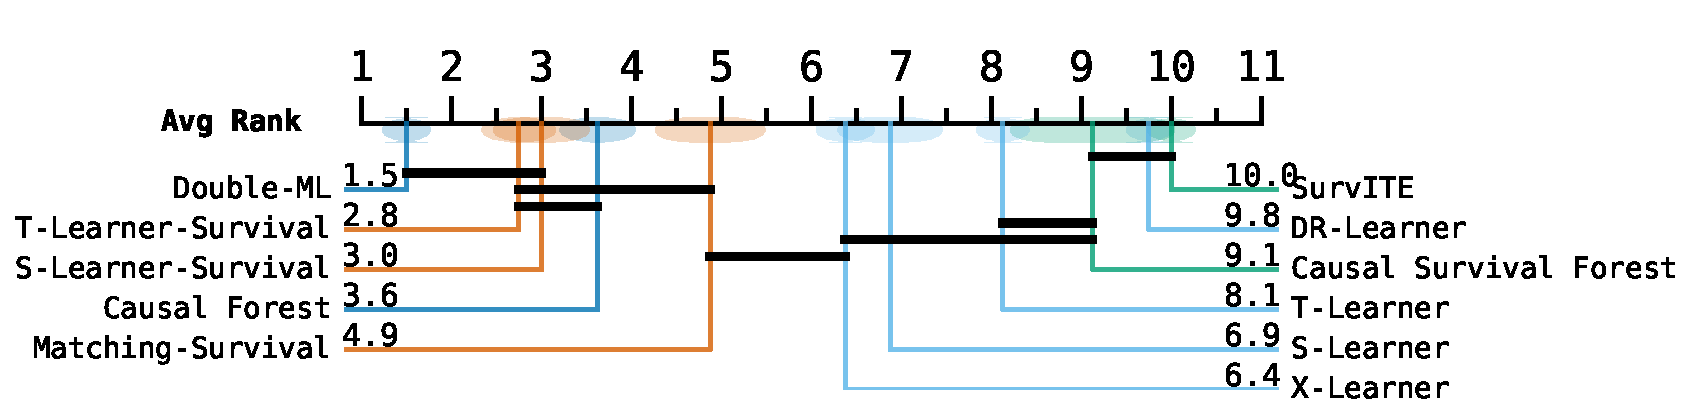
\includegraphics[width=\linewidth]{Appendices/appendix-ch04/images/figure_results_updated/average_ranks/average_ranking_visualization_method_combination_scenario_A.pdf}
        \centering
        
    \end{minipage}}
    \hfill
    \subfloat[{Scenario \texttt{B}}]{\begin{minipage}[t]{0.49\textwidth}
        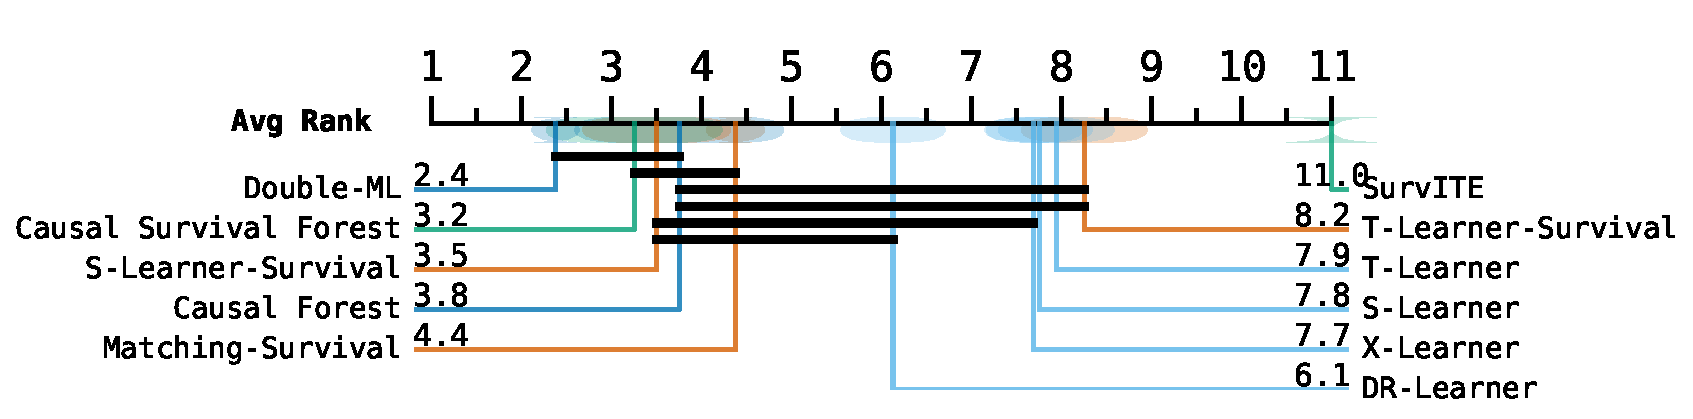
\includegraphics[width=\linewidth]{Appendices/appendix-ch04/images/figure_results_updated/average_ranks/average_ranking_visualization_method_combination_scenario_B.pdf}
        \centering
        
    \end{minipage}}

    

    \subfloat[{Scenario \texttt{C}}]{\begin{minipage}[t]{0.49\textwidth}
        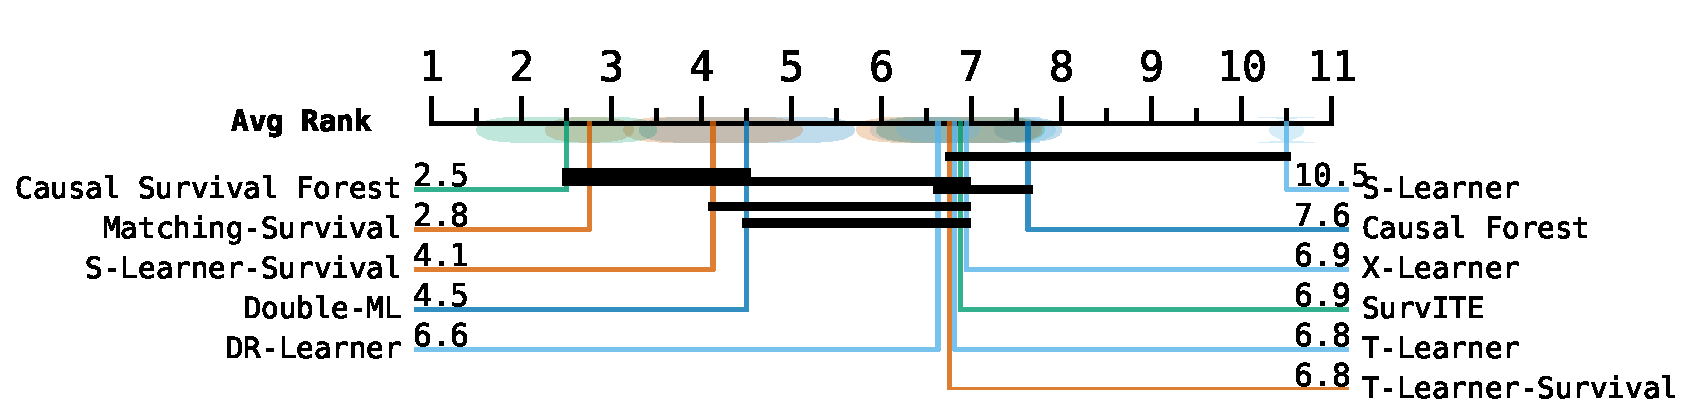
\includegraphics[width=\linewidth]{Appendices/appendix-ch04/images/figure_results_updated/average_ranks/average_ranking_visualization_method_combination_scenario_C.pdf}
        \centering
        
    \end{minipage}}
    \hfill
    \subfloat[{Scenario \texttt{D}}]{\begin{minipage}[t]{0.49\textwidth}
        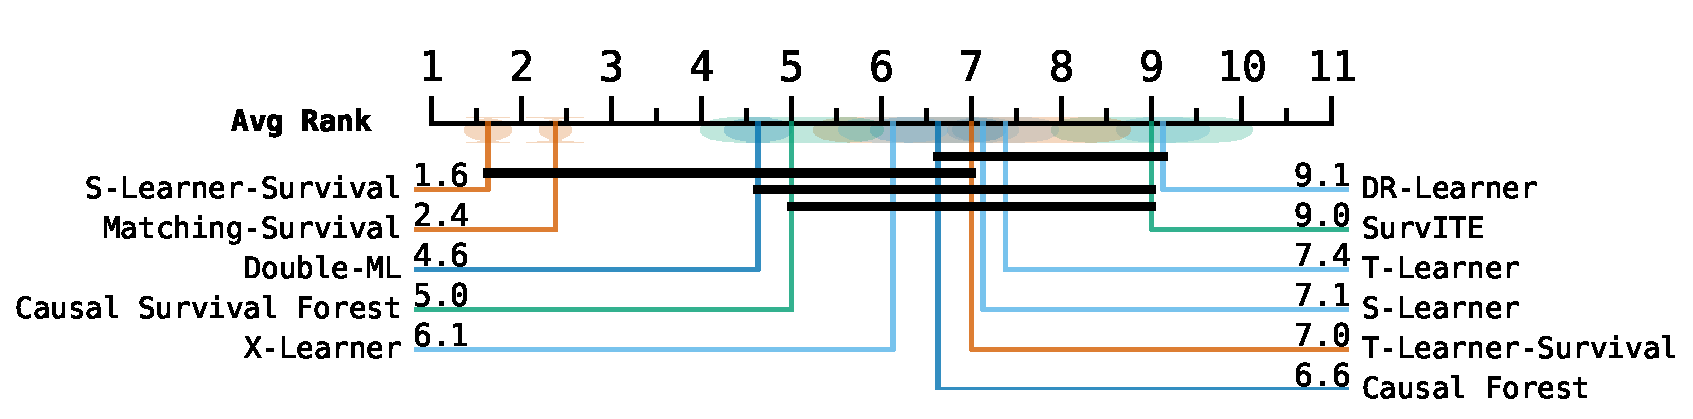
\includegraphics[width=\linewidth]{Appendices/appendix-ch04/images/figure_results_updated/average_ranks/average_ranking_visualization_method_combination_scenario_D.pdf}
        \centering
        
    \end{minipage}}

    

    \subfloat[{Scenario \texttt{E}}]{\begin{minipage}[t]{0.49\textwidth}
        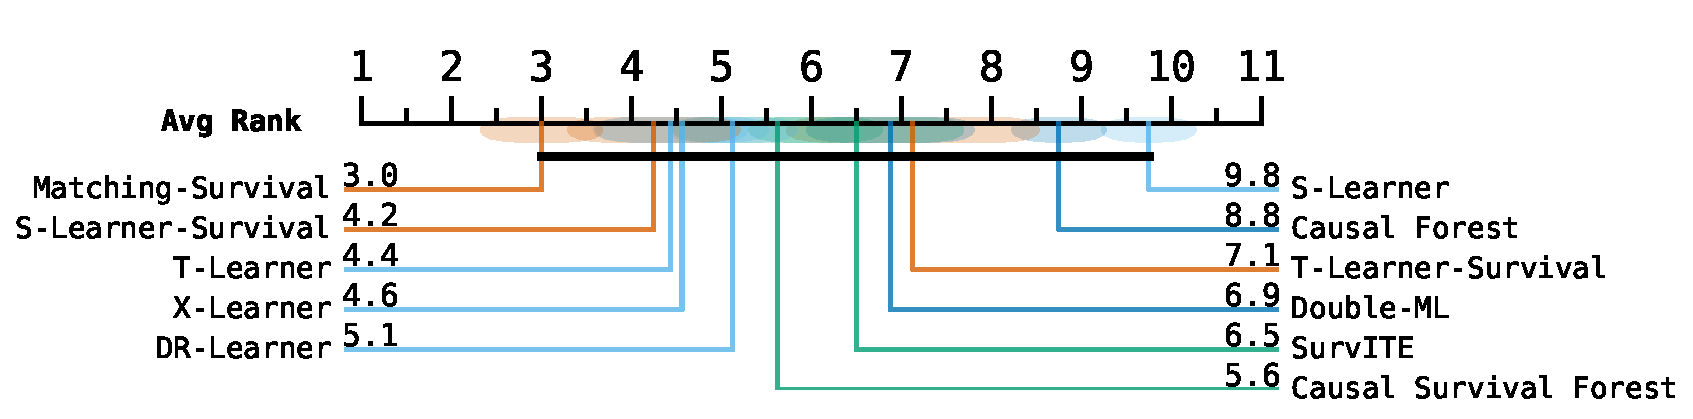
\includegraphics[width=\linewidth]{Appendices/appendix-ch04/images/figure_results_updated/average_ranks/average_ranking_visualization_method_combination_scenario_E.pdf}
        \centering
        
    \end{minipage}}

    \hfill

    
    
}
\end{figure}



% \ChFourRebuttal{In addition to the global rankings in Figure~\ref{ch04:fig:average_rank_per_scenario}, we report scenario-specific win-rates in Table~\ref{ch04:tab:scenario-winrates}. For each survival scenario (\texttt{A}--\texttt{E}), we compute how often each method family appears in the Top-1, Top-3, and Top-5 positions for CATE RMSE and \textcolor{black}{ATE Bias} across the eight causal configurations. This allows us to examine how the relative advantages of outcome imputation, direct-survival, and survival meta-learner approaches change as we vary both the survival time model (Cox, AFT, Poisson) and the censoring rate (low, medium, high; Table~\ref{ch04:tab:synthetic-data-survival-scenario}).}
\ChFourRebuttal{In addition to the global rankings in Figure~\ref{ch04:fig:average_rank_per_scenario}, we report scenario-specific win-rates in Table~\ref{ch04:tab:scenario-winrates}. For each survival scenario (\texttt{A}--\texttt{E}), we compute how often each method family appears in the Top-1, Top-3, and Top-5 positions for CATE RMSE and ATE Bias across the eight causal configurations. This provides a complementary view of robustness, highlighting which families consistently occupy the top ranks as we vary the survival time model (Cox, AFT, Poisson) and the censoring rate (low, medium, high; Table~\ref{ch04:tab:synthetic-data-survival-scenario}).}


% \ChFourRebuttal{Under low censoring (Scenarios~\texttt{A} and~\texttt{B}), outcome regression methods remain competitive, but their strengths are scenario-dependent. In Scenario~\texttt{A} (Cox, low censoring), Double-ML dominates CATE RMSE with a 100\% Top-1/Top-3/Top-5 win-rate, while Causal Forest is almost always in the Top-3 and Top-5. \textcolor{black}{ATE Bias is more dispersed}: SurvITE, DR-Learner, and several meta-learners share Top-1 and Top-3 positions, and Causal Survival Forests is frequently among the top methods. In Scenario~\texttt{B} (AFT, low censoring), Causal Survival Forests becomes the main winner, achieving the highest CATE RMSE win-rates (62.5\% Top-1 and 100\% Top-3/Top-5) and strong ATE Bias performance, with Double-ML and Causal Forest also appearing often in the Top-3 and Top-5.}
\ChFourRebuttal{Under low censoring (Scenarios~\texttt{A} and~\texttt{B}), outcome-imputation approaches can still be competitive on CATE RMSE, but the winners are scenario-dependent and survival-aware methods remain highly prevalent in the Top-$k$ sets. In Scenario~\texttt{A} (Cox, low censoring), Double-ML dominates CATE RMSE (62.5\% Top-1 and 100\% Top-3/Top-5), while survival meta-learners also appear frequently in Top-3/Top-5 (e.g., T-Learner-Survival and S-Learner-Survival are both 100\% Top-5). ATE Bias is more dispersed: S-Learner and DR-Learner each attain 25.0\% Top-1, and survival meta-learners (S-Learner-Survival and Matching-Survival) contribute strongly to Top-3/Top-5, whereas the direct-survival CATE methods have limited presence. In Scenario~\texttt{B} (AFT, low censoring), Causal Survival Forests becomes a leading family for both metrics (37.5\% Top-1 CATE RMSE; 25.0\% Top-1 ATE Bias; 75.0\% Top-3/Top-5 ATE Bias). At the same time, Causal Forest remains competitive on CATE RMSE (37.5\% Top-1), and survival meta-learners retain substantial Top-5 coverage, particularly Matching-Survival (87.5\% Top-5 CATE RMSE) and S-Learner-Survival (87.5\% Top-5 CATE RMSE). Notably, SurvITE does not appear among the Top-$k$ in this scenario.}

% \ChFourRebuttal{As censoring increases, survival-specific modeling becomes more important. In Scenario~\texttt{C} (Poisson, medium censoring), Causal Survival Forests clearly leads in both CATE RMSE and ATE Bias, with Double-ML and SurvITE providing additional support in the Top-3 and Top-5. Under high censoring (Scenarios~\texttt{D} and~\texttt{E}), the advantage of survival-focused methods is even more pronounced. In Scenario~\texttt{D} (AFT, high censoring), SurvITE and the survival meta-learners (S-Learner-Survival, Matching-Survival, and T-Learner-Survival) capture most Top-1 and Top-3 spots in CATE RMSE, while Causal Survival Forests and the same survival meta-learners dominate ATE Bias. In Scenario~\texttt{E} (Poisson, high censoring), Causal Survival Forests and the survival meta-learners again account for nearly all Top-1 and Top-3 positions for both metrics, with Double-ML mainly contributing through Top-5 appearances. Across these settings, classical meta-learners without survival structure rarely win, reinforcing that explicit survival modeling is crucial once censoring becomes moderate or high.}
\ChFourRebuttal{As censoring increases, survival-specific modeling becomes increasingly important and accounts for a larger fraction of the best-performing sets. In Scenario~\texttt{C} (Poisson, medium censoring), Causal Survival Forests clearly leads on both metrics (62.5\% Top-1 CATE RMSE; 37.5\% Top-1 ATE Bias; 100\% Top-5 ATE Bias), while Matching-Survival and S-Learner-Survival frequently appear among the best methods (e.g., Matching-Survival is 25.0\% Top-1 CATE RMSE and 100\% Top-5 CATE RMSE; both Matching-Survival and S-Learner-Survival reach 75.0\% Top-3 CATE RMSE). Under high censoring, the dominance shifts even more strongly toward survival-aware families, but with different emphases across scenarios. In Scenario~\texttt{D} (AFT, high censoring), S-Learner-Survival is the primary winner on CATE RMSE (50.0\% Top-1 and 100\% Top-3/Top-5), while Matching-Survival achieves perfect Top-3/Top-5 coverage (100\% in both cases). For ATE Bias, the top positions are shared across multiple survival-aware families (Causal Survival Forests, T-Learner-Survival, and S-Learner-Survival each at 25.0\% Top-1). In Scenario~\texttt{E} (Poisson, high censoring), the strongest ATE Bias performance is achieved by T-Learner-Survival (50.0\% Top-1 and 87.5\% Top-5), with Matching-Survival and SurvITE following, whereas CATE RMSE Top-1 is more distributed (Matching-Survival: 37.5\% Top-1; several other methods across both outcome-imputation and direct-survival CATE methods at 12.5\%). Overall, across all scenarios, classical outcome-imputation methods are rarely dominant or ranked Top-1 under moderate or high censoring, reinforcing the benefit of explicitly modeling time-to-event structure when the censoring rate is high.}


% !TeX root = ../../../main.tex
\begin{table}[htbp]
\ChFourFloatContents{ch04:tab:scenario-winrates}{\caption{\ChFourRebuttal{Win-rate (\%) of method families by Survival Scenario. 
Values denote the percentage of times a method appears in the Top-1, Top-3, and Top-5 
according to CATE RMSE and ATE Bias across the eight causal configurations for each scenario.}}}{
\centering



\begin{minipage}{0.48\textwidth}
\centering
\textbf{Scenario \texttt{A}: Cox, Low Censoring}\\[0.25em]
\begin{adjustbox}{max width=\textwidth}
\begin{tabular}{lccc@{\hspace{18pt}}ccc}
\toprule
\multirow{2}{*}{\textbf{Method Family}} &
\multicolumn{3}{c}{\textbf{CATE RMSE}} &
\multicolumn{3}{c}{\textbf{ATE Bias}} \\
\cmidrule(lr){2-4} \cmidrule(lr){5-7}
& \textbf{Top-1} & \textbf{Top-3} & \textbf{Top-5}
& \textbf{Top-1} & \textbf{Top-3} & \textbf{Top-5} \\
\midrule
\multicolumn{7}{l}{\textit{Outcome Imputation Methods}} \\
T-Learner               & \textcolor{gray}{0}   & \textcolor{gray}{0}   & \textcolor{gray}{0}   & \textcolor{gray}{0}   & 25.0 & 25.0 \\
S-Learner               & \textcolor{gray}{0}   & 12.5 & 12.5 & 25.0 & 50.0 & 50.0 \\
X-Learner               & \textcolor{gray}{0}   & \textcolor{gray}{0}   & 12.5 & \textcolor{gray}{0}   & 25.0 & 62.5 \\
DR-Learner              & \textcolor{gray}{0}   & \textcolor{gray}{0}   & \textcolor{gray}{0}   & 25.0 & 25.0 & 62.5 \\
Double-ML               & 62.5 & 100.0 & 100.0 & \textcolor{gray}{0}   & 12.5 & 37.5 \\
Causal Forest           & \textcolor{gray}{0}   & 37.5 & 100.0 & 12.5 & 12.5 & 37.5 \\
\addlinespace %
\multicolumn{7}{l}{\textit{Direct-Survival CATE Methods}} \\
Causal Survival Forests  & \textcolor{gray}{0}   & \textcolor{gray}{0}   & \textcolor{gray}{0}   & \textcolor{gray}{0}   & 12.5 & 25.0 \\
SurvITE                 & \textcolor{gray}{0}   & \textcolor{gray}{0}   & \textcolor{gray}{0}   & \textcolor{gray}{0}   & \textcolor{gray}{0}   & 25.0 \\
\addlinespace %
\multicolumn{7}{l}{\textit{Survival Meta-Learners}} \\
T-Learner-Survival      & 12.5 & 87.5 & 100.0 & 12.5 & 25.0 & 50.0 \\
S-Learner-Survival      & 25.0 & 50.0 & 100.0 & 12.5 & 62.5 & 75.0 \\
Matching-Survival       & \textcolor{gray}{0}   & 12.5 & 75.0 & 12.5 & 50.0 & 50.0 \\
\bottomrule
\end{tabular}
\end{adjustbox}
\end{minipage}
\hfill
\begin{minipage}{0.48\textwidth}
\centering
\textbf{Scenario \texttt{B}: AFT, Low Censoring}\\[0.25em]
\begin{adjustbox}{max width=\textwidth}
\begin{tabular}{lccc@{\hspace{18pt}}ccc}
\toprule
\multirow{2}{*}{\textbf{Method Family}} &
\multicolumn{3}{c}{\textbf{CATE RMSE}} &
\multicolumn{3}{c}{\textbf{ATE Bias}} \\
\cmidrule(lr){2-4} \cmidrule(lr){5-7}
& \textbf{Top-1} & \textbf{Top-3} & \textbf{Top-5}
& \textbf{Top-1} & \textbf{Top-3} & \textbf{Top-5} \\
\midrule
\multicolumn{7}{l}{\textit{Outcome Imputation Methods}} \\
T-Learner               & \textcolor{gray}{0}   & \textcolor{gray}{0}   & 12.5 & \textcolor{gray}{0}   & 12.5 & 25.0 \\
S-Learner               & \textcolor{gray}{0}   & \textcolor{gray}{0}   & \textcolor{gray}{0}   & \textcolor{gray}{0}   & 12.5 & 25.0 \\
X-Learner               & \textcolor{gray}{0}   & \textcolor{gray}{0}   & 12.5 & 12.5 & 12.5 & 37.5 \\
DR-Learner              & \textcolor{gray}{0}   & 12.5 & 25.0 & \textcolor{gray}{0}   & 25.0 & 37.5 \\
Double-ML               & 12.5 & 100.0 & 100.0 & 12.5 & 12.5 & 37.5 \\
Causal Forest           & 37.5 & 50.0 & 75.0 & \textcolor{gray}{0}   & 25.0 & 62.5 \\
\addlinespace %
\multicolumn{7}{l}{\textit{Direct-Survival CATE Methods}} \\
Causal Survival Forests  & 37.5 & 62.5 & 87.5 & 25.0 & 75.0 & 75.0 \\
SurvITE                 & \textcolor{gray}{0}   & \textcolor{gray}{0}   & \textcolor{gray}{0}   & \textcolor{gray}{0}   & \textcolor{gray}{0}   & \textcolor{gray}{0} \\
\addlinespace %
\multicolumn{7}{l}{\textit{Survival Meta-Learners}} \\
T-Learner-Survival      & \textcolor{gray}{0}   & \textcolor{gray}{0}   & 12.5 & 25.0 & 37.5 & 62.5 \\
S-Learner-Survival      & 12.5 & 62.5 & 87.5 & 12.5 & 37.5 & 62.5 \\
Matching-Survival       & \textcolor{gray}{0}   & 12.5 & 87.5 & 12.5 & 50.0 & 75.0 \\
\bottomrule
\end{tabular}
\end{adjustbox}
\end{minipage}



\begin{minipage}{0.48\textwidth}
\centering
\textbf{Scenario \texttt{C}: Poisson, Medium Censoring}\\[0.25em]
\begin{adjustbox}{max width=\textwidth}
\begin{tabular}{lccc@{\hspace{18pt}}ccc}
\toprule
\multirow{2}{*}{\textbf{Method Family}} &
\multicolumn{3}{c}{\textbf{CATE RMSE}} &
\multicolumn{3}{c}{\textbf{ATE Bias}} \\
\cmidrule(lr){2-4} \cmidrule(lr){5-7}
& \textbf{Top-1} & \textbf{Top-3} & \textbf{Top-5}
& \textbf{Top-1} & \textbf{Top-3} & \textbf{Top-5} \\
\midrule
\multicolumn{7}{l}{\textit{Outcome Imputation Methods}} \\
T-Learner               & \textcolor{gray}{0}   & 25.0 & 37.5 & \textcolor{gray}{0}   & 12.5 & 25.0 \\
S-Learner               & \textcolor{gray}{0}   & \textcolor{gray}{0}   & \textcolor{gray}{0}   & \textcolor{gray}{0}   & \textcolor{gray}{0}   & \textcolor{gray}{0} \\
X-Learner               & \textcolor{gray}{0}   & 25.0 & 37.5 & \textcolor{gray}{0}   & \textcolor{gray}{0}   & 25.0 \\
DR-Learner              & \textcolor{gray}{0}   & \textcolor{gray}{0}   & 25.0 & \textcolor{gray}{0}   & \textcolor{gray}{0}   & \textcolor{gray}{0} \\
Double-ML               & 12.5 & 50.0 & 62.5 & \textcolor{gray}{0}   & \textcolor{gray}{0}   & \textcolor{gray}{0} \\
Causal Forest           & \textcolor{gray}{0}   & \textcolor{gray}{0}   & \textcolor{gray}{0}   & \textcolor{gray}{0}   & \textcolor{gray}{0}   & \textcolor{gray}{0} \\
\addlinespace %
\multicolumn{7}{l}{\textit{Direct-Survival CATE Methods}} \\
Causal Survival Forests  & 62.5 & 75.0 & 87.5 & 37.5 & 75.0 & 100.0 \\
SurvITE                 & \textcolor{gray}{0}   & \textcolor{gray}{0}   & 50.0 & 25.0 & 50.0 & 87.5 \\
\addlinespace %
\multicolumn{7}{l}{\textit{Survival Meta-Learners}} \\
T-Learner-Survival      & \textcolor{gray}{0}   & 12.5 & 25.0 & 12.5 & 25.0 & 75.0 \\
S-Learner-Survival      & \textcolor{gray}{0}   & 62.5 & 75.0 & \textcolor{gray}{0}   & 62.5 & 100.0 \\
Matching-Survival       & 25.0 & 75.0 & 100.0 & 25.0 & 75.0 & 87.5 \\
\bottomrule
\end{tabular}
\end{adjustbox}
\end{minipage}
\hfill
\begin{minipage}{0.48\textwidth}
\centering
\textbf{Scenario \texttt{D}: AFT, High Censoring}\\[0.25em]
\begin{adjustbox}{max width=\textwidth}
\begin{tabular}{lccc@{\hspace{18pt}}ccc}
\toprule
\multirow{2}{*}{\textbf{Method Family}} &
\multicolumn{3}{c}{\textbf{CATE RMSE}} &
\multicolumn{3}{c}{\textbf{ATE Bias}} \\
\cmidrule(lr){2-4} \cmidrule(lr){5-7}
& \textbf{Top-1} & \textbf{Top-3} & \textbf{Top-5}
& \textbf{Top-1} & \textbf{Top-3} & \textbf{Top-5} \\
\midrule
\multicolumn{7}{l}{\textit{Outcome Imputation Methods}} \\
T-Learner               & \textcolor{gray}{0}   & \textcolor{gray}{0}   & 25.0 & 12.5 & 12.5 & 50.0 \\
S-Learner               & \textcolor{gray}{0}   & \textcolor{gray}{0}   & \textcolor{gray}{0}   & \textcolor{gray}{0}   & 12.5 & 50.0 \\
X-Learner               & \textcolor{gray}{0}   & \textcolor{gray}{0}   & 37.5 & 12.5 & 12.5 & 25.0 \\
DR-Learner              & \textcolor{gray}{0}   & \textcolor{gray}{0}   & \textcolor{gray}{0}   & \textcolor{gray}{0}   & 12.5 & 37.5 \\
Double-ML               & \textcolor{gray}{0}   & \textcolor{gray}{0}   & 87.5 & \textcolor{gray}{0}   & \textcolor{gray}{0}   & 12.5 \\
Causal Forest           & \textcolor{gray}{0}   & \textcolor{gray}{0}   & 37.5 & \textcolor{gray}{0}   & \textcolor{gray}{0}   & 37.5 \\
\addlinespace %
\multicolumn{7}{l}{\textit{Direct-Survival CATE Methods}} \\
Causal Survival Forests  & 12.5 & 50.0 & 50.0 & 25.0 & 62.5 & 87.5 \\
SurvITE                 & \textcolor{gray}{0}   & 12.5 & 25.0 & \textcolor{gray}{0}   & 12.5 & 12.5 \\
\addlinespace %
\multicolumn{7}{l}{\textit{Survival Meta-Learners}} \\
T-Learner-Survival      & 37.5 & 37.5 & 37.5 & 25.0 & 25.0 & 37.5 \\
S-Learner-Survival      & 50.0 & 100.0 & 100.0 & 25.0 & 75.0 & 75.0 \\
Matching-Survival       & \textcolor{gray}{0}   & 100.0 & 100.0 & 12.5 & 75.0 & 75.0 \\
\bottomrule
\end{tabular}
\end{adjustbox}
\end{minipage}



\begin{minipage}{0.48\textwidth}
\centering
\textbf{Scenario \texttt{E}: Poisson, High Censoring}\\[0.25em]
\begin{adjustbox}{max width=\textwidth}
\begin{tabular}{lccc@{\hspace{18pt}}ccc}
\toprule
\multirow{2}{*}{\textbf{Method Family}} &
\multicolumn{3}{c}{\textbf{CATE RMSE}} &
\multicolumn{3}{c}{\textbf{ATE Bias}} \\
\cmidrule(lr){2-4} \cmidrule(lr){5-7}
& \textbf{Top-1} & \textbf{Top-3} & \textbf{Top-5}
& \textbf{Top-1} & \textbf{Top-3} & \textbf{Top-5} \\
\midrule
\multicolumn{7}{l}{\textit{Outcome Imputation Methods}} \\
T-Learner               & 12.5 & 37.5 & 75.0 & \textcolor{gray}{0}   & 12.5 & 37.5 \\
S-Learner               & \textcolor{gray}{0}   & \textcolor{gray}{0}   & \textcolor{gray}{0}   & \textcolor{gray}{0}   & \textcolor{gray}{0}   & \textcolor{gray}{0} \\
X-Learner               & 12.5 & 37.5 & 75.0 & \textcolor{gray}{0}   & 37.5 & 50.0 \\
DR-Learner              & \textcolor{gray}{0}   & 25.0 & 62.5 & \textcolor{gray}{0}   & \textcolor{gray}{0}   & 12.5 \\
Double-ML               & 12.5 & 12.5 & 12.5 & \textcolor{gray}{0}   & \textcolor{gray}{0}   & \textcolor{gray}{0} \\
Causal Forest           & \textcolor{gray}{0}   & \textcolor{gray}{0}   & \textcolor{gray}{0}   & \textcolor{gray}{0}   & \textcolor{gray}{0}   & \textcolor{gray}{0} \\
\addlinespace %
\multicolumn{7}{l}{\textit{Direct-Survival CATE Methods}} \\
Causal Survival Forests  & 12.5 & 37.5 & 37.5 & \textcolor{gray}{0}   & 37.5 & 87.5 \\
SurvITE                 & 12.5 & 12.5 & 37.5 & 12.5 & 50.0 & 75.0 \\
\addlinespace %
\multicolumn{7}{l}{\textit{Survival Meta-Learners}} \\
T-Learner-Survival      & 12.5 & 25.0 & 37.5 & 50.0 & 75.0 & 87.5 \\
S-Learner-Survival      & \textcolor{gray}{0}   & 62.5 & 62.5 & 12.5 & 50.0 & 75.0 \\
Matching-Survival       & 37.5 & 50.0 & 100.0 & 25.0 & 37.5 & 75.0 \\
\bottomrule
\end{tabular}
\end{adjustbox}
\end{minipage}

}
\end{table}






%%%%%%%%%%%%%%%%%%%%%%%%%%%%%%%%%%%%%%%%%%%%%%%%%%%%%%%%%%%%
%%%%%%%%%%%%%%%%%%%%%%%%%%%%%%%%%%%%%%%%%%%%%%%%%%%%%%%%%%%%
%%%%%%%%%%%%%%%%%%%%%%%%%%%%%%%%%%%%%%%%%%%%%%%%%%%%%%%%%%%%

\subsubsection{Ranking of causal methods for different Causal Configurations}
\label{ch04:app:more-avg-rank}

% In Figure~\ref{ch04:fig:average_rank_per_experiments}, we present the Borda ranking of causal model families across eight distinct causal configurations, each representing different combinations of assumptions related to treatment assignment (RCT vs. observational), ignorability, positivity, and censoring mechanisms. Within each configuration, the average rank of each method is computed over all survival scenarios, allowing us to isolate how assumption violations affect model performance independently of survival data characteristics.
In Figure~\ref{ch04:fig:average_rank_per_experiments}, we present the Borda ranking of causal model families across eight distinct causal configurations, each representing different combinations of assumptions related to treatment assignment (RCT vs. observational), ignorability, positivity, and censoring mechanisms. Within each configuration, the average rank of each method is computed over all survival scenarios, allowing us to isolate how assumption violations affect model performance independently of survival data characteristics.
The colors of the lines connecting the methods to the horizontal axis represent the specific family of the method (e.g., outcome imputation based, direct-survival CATE, survival meta-learners).

% Notably, outcome imputation approaches such as X-Learner and Double-ML perform best in randomized settings with unbalanced treatment (e.g., RCT-5\%, panel b), but their performance deteriorates as we move to settings with unmeasured confounding, or more visibly with informative-censoring. In contrast, survival-specific methods such as S-Learner-Survival, Matching-Survival, and Causal Survival Forests consistently rise in the rankings under these challenging conditions--particularly when multiple violations occur simultaneously (e.g., panel g and h). This trend suggests that survival meta-learners and direct modeling of the survival process offer increased robustness to violations of standard causal assumptions, especially in the presence of unmeasured confounding and informative censoring. 
% Another finding here is that Causal Survival Forests maintains strong performance across many configurations, consistently ranking in the top half--particularly in settings involving unmeasured confounding or informative censoring. However, when the positivity assumption is violated (e.g., Figure~\ref{ch04:fig:average_rank_per_experiments}e and h), its performance declines, suggesting limitations in modeling highly sparse regions of the covariate space with deterministic treatment assignment.
Notably, outcome imputation approaches perform best in randomized settings with unbalanced treatment (e.g., RCT-5\%, Figure~\ref{ch04:fig:borda_ranking_causal_config_RCT_05}), where Double-ML achieves the top rank of 1.80.
However, their performance deteriorates as we move to settings with unmeasured confounding (Figure~\ref{ch04:fig:borda_ranking_causal_config_OBS_UConf}), or more visibly with informative censoring (Figures~\ref{ch04:fig:borda_ranking_causal_config_OBS_InfC},~\ref{ch04:fig:borda_ranking_causal_config_OBS_UConf_InfC},~\ref{ch04:fig:borda_ranking_causal_config_OBS_NoPos_InfC}), where Double-ML drops to the bottom of the top half and X-Learner falls entirely into the lower-performing half of the rankings.
In contrast, survival-specific methods of survival meta-learners such as S-Learner-Survival, Matching-Survival, and Causal Survival Forests (belonging to the direct-survival CATE family) consistently rise in the rankings under these conditions, particularly when multiple violations occur simultaneously (e.g., Figures~\ref{ch04:fig:borda_ranking_causal_config_OBS_UConf_InfC},~\ref{ch04:fig:borda_ranking_causal_config_OBS_NoPos_InfC}), where S-Learner-Survival and Matching-Survival take the top two spots.
This trend suggests that survival meta-learners and Causal Survival Forests, which directly model the survival process, offer increased robustness to violations of standard causal assumptions, especially in the presence of unmeasured confounding and informative censoring.
Another finding is that Causal Survival Forests maintains strong performance across many configurations, consistently ranking in the top half---particularly in settings involving informative censoring (e.g., Figures~\ref{ch04:fig:borda_ranking_causal_config_OBS_InfC},~\ref{ch04:fig:borda_ranking_causal_config_OBS_UConf_InfC}).
However, when the positivity assumption is violated while censoring remains ignorable (Figure~\ref{ch04:fig:borda_ranking_causal_config_OBS_NoPos}), its performance declines substantially, dropping to a rank of 6.60 in the bottom half of the ranking.
This suggests limitations in modeling highly sparse regions of the covariate space with deterministic treatment assignment under certain censoring conditions.


% !TeX root = ../../../main.tex
\begin{figure}[htbp]
\ChFourFloatContents{ch04:fig:average_rank_per_experiments}{\caption{Average ranking of each model for each causal configuration. \ChFourRebuttal{Shaded regions indicate the standard error of the rank across datasets.}}}{
    \centering

    \subfloat[{RCT: \ChFourGrayCheck (50\%), Ignorability: \ChFourGrayCheck, Positivity: \ChFourGrayCheck, Ign-Censoring: \ChFourGrayCheck}]{\begin{minipage}[t]{0.49\textwidth}
        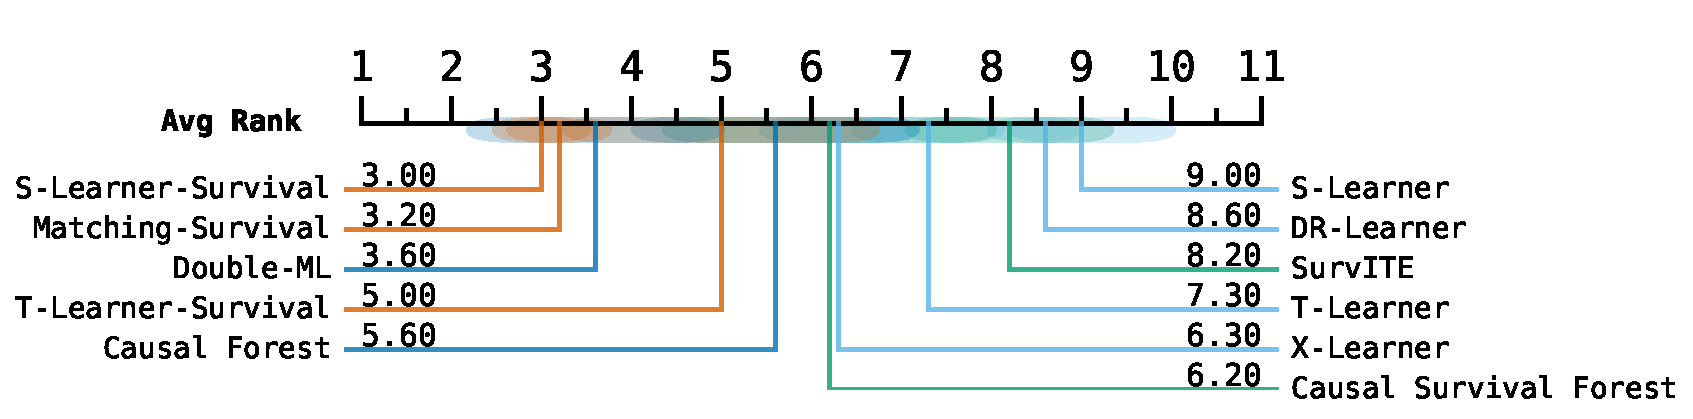
\includegraphics[width=\linewidth]{Appendices/appendix-ch04/images/figure_results_updated/average_ranks/average_ranking_visualization_method_combination_RCT-50.pdf}
        \centering
        
        \label{ch04:fig:borda_ranking_causal_config_RCT_50}
    \end{minipage}}
    \hfill
    \subfloat[{RCT: \ChFourGrayCheck (5\%), Ignorability: \ChFourGrayCheck, Positivity: \ChFourGrayCheck, Ign-Censoring: \ChFourGrayCheck}]{\begin{minipage}[t]{0.49\textwidth}
        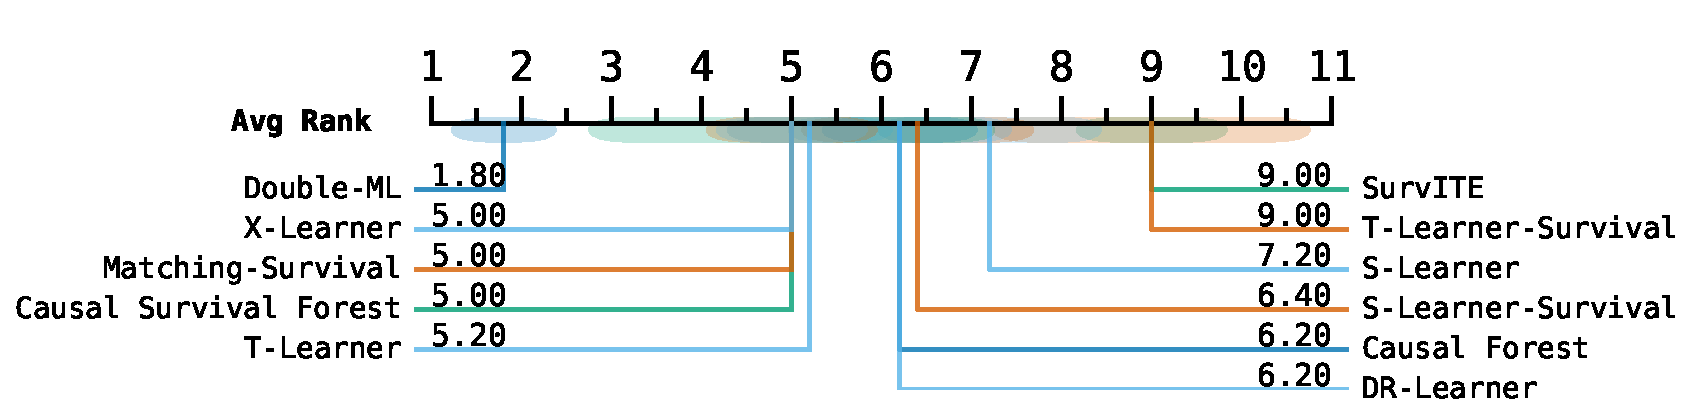
\includegraphics[width=\linewidth]{Appendices/appendix-ch04/images/figure_results_updated/average_ranks/average_ranking_visualization_method_combination_RCT-5.pdf}
        \centering
        
        \label{ch04:fig:borda_ranking_causal_config_RCT_05}
    \end{minipage}}

    

    \subfloat[{RCT: \ChFourBlackCross, Ignorability: \ChFourGrayCheck, Positivity: \ChFourGrayCheck, Ignorable Censoring: \ChFourGrayCheck}]{\begin{minipage}[t]{0.49\textwidth}
        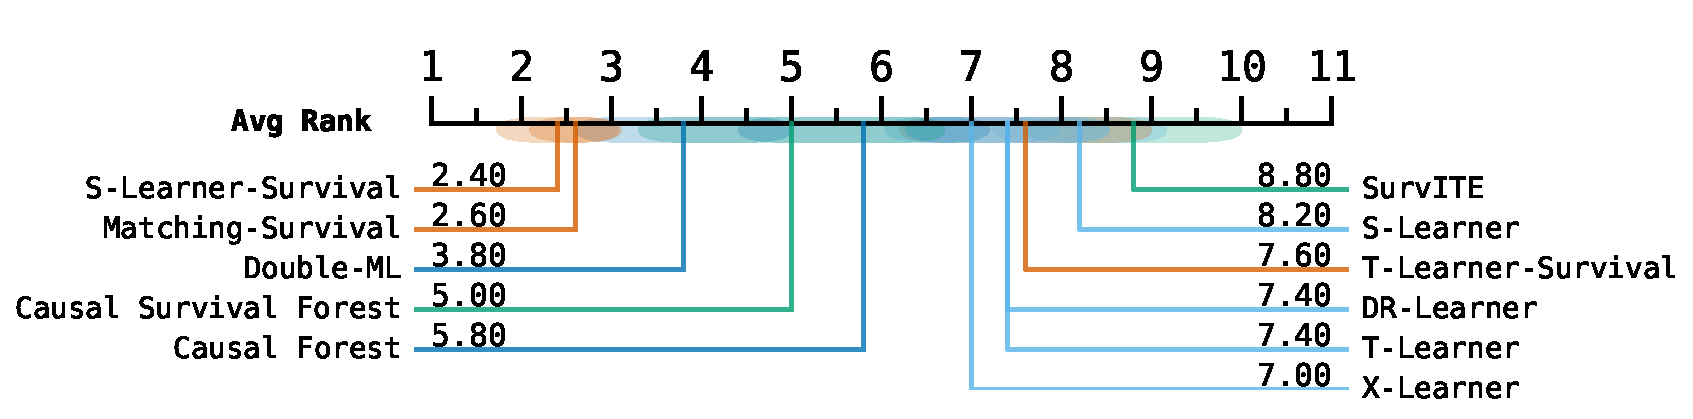
\includegraphics[width=\linewidth]{Appendices/appendix-ch04/images/figure_results_updated/average_ranks/average_ranking_visualization_method_combination_OBS-CPS.pdf}
        \centering
        
        \label{ch04:fig:borda_ranking_causal_config_OBS_CPS}
    \end{minipage}}
    \hfill
    \subfloat[{RCT: \ChFourBlackCross, Ignorability: \ChFourBlackCross, Positivity: \ChFourGrayCheck, Ignorable Censoring: \ChFourGrayCheck}]{\begin{minipage}[t]{0.49\textwidth}
        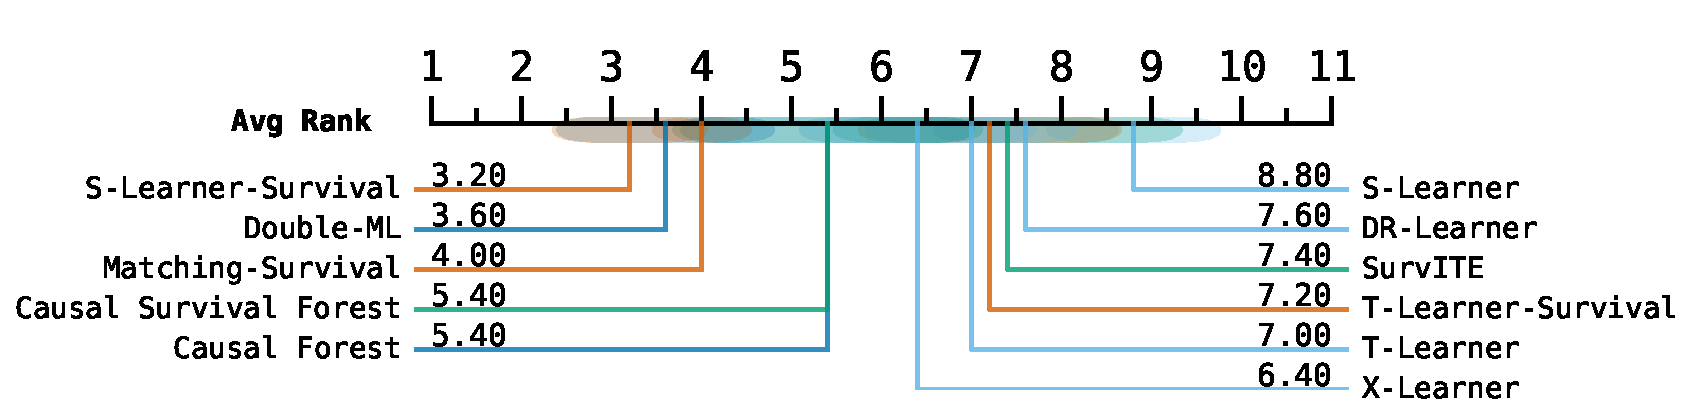
\includegraphics[width=\linewidth]{Appendices/appendix-ch04/images/figure_results_updated/average_ranks/average_ranking_visualization_method_combination_OBS-UConf.pdf}
        \centering
        
        \label{ch04:fig:borda_ranking_causal_config_OBS_UConf}
    \end{minipage}}

    

    \subfloat[{RCT: \ChFourBlackCross, Ignorability: \ChFourGrayCheck, Positivity: \ChFourBlackCross, Ignorable Censoring: \ChFourGrayCheck}]{\begin{minipage}[t]{0.49\textwidth}
        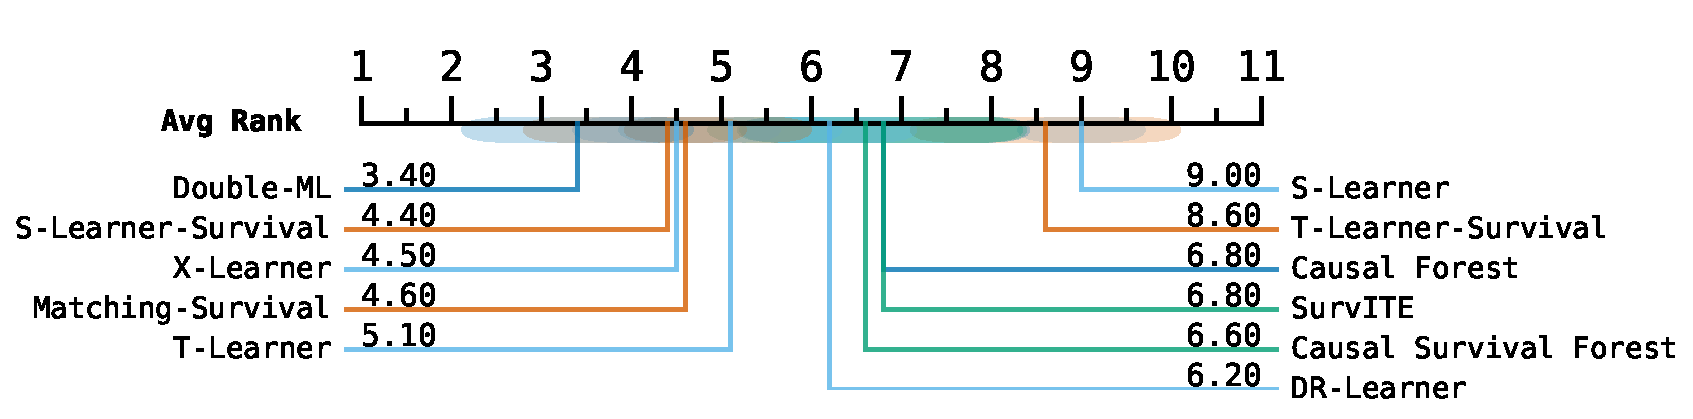
\includegraphics[width=\linewidth]{Appendices/appendix-ch04/images/figure_results_updated/average_ranks/average_ranking_visualization_method_combination_OBS-NoPos.pdf}
        \centering
        
        \label{ch04:fig:borda_ranking_causal_config_OBS_NoPos}
    \end{minipage}}
    \hfill
    \subfloat[{RCT: \ChFourBlackCross, Ignorability: \ChFourGrayCheck, Positivity: \ChFourGrayCheck, Ignorable Censoring: \ChFourBlackCross}]{\begin{minipage}[t]{0.49\textwidth}
        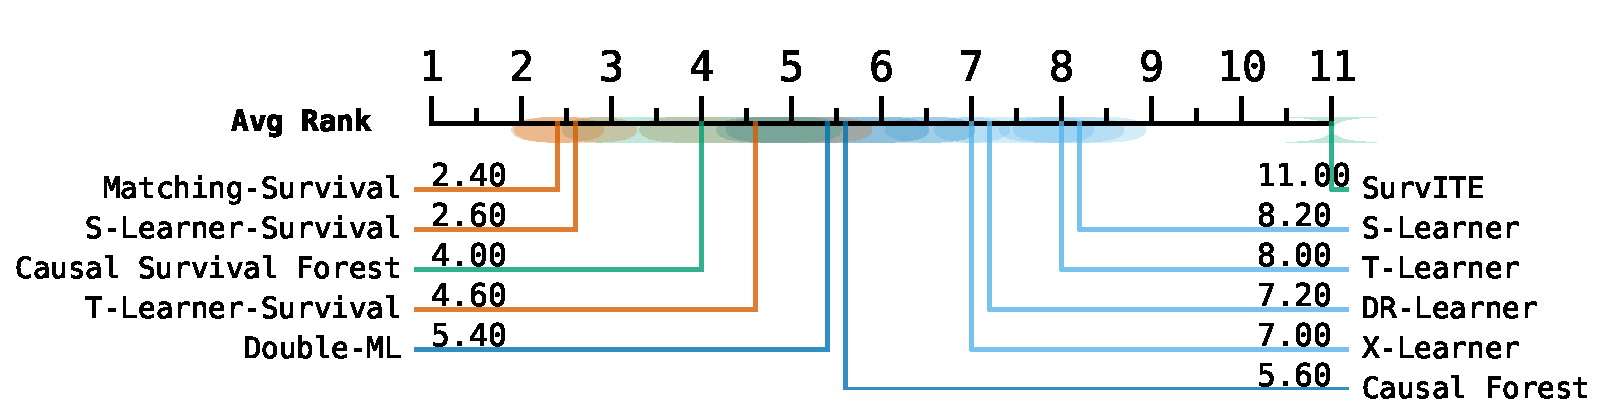
\includegraphics[width=\linewidth]{Appendices/appendix-ch04/images/figure_results_updated/average_ranks/average_ranking_visualization_method_combination_OBS-CPS-IC.pdf}
        \centering
        
        \label{ch04:fig:borda_ranking_causal_config_OBS_InfC}
    \end{minipage}}

    

    \subfloat[{RCT: \ChFourBlackCross, Ignorability: \ChFourBlackCross, Positivity: \ChFourGrayCheck, Ignorable Censoring: \ChFourBlackCross}]{\begin{minipage}[t]{0.49\textwidth}
        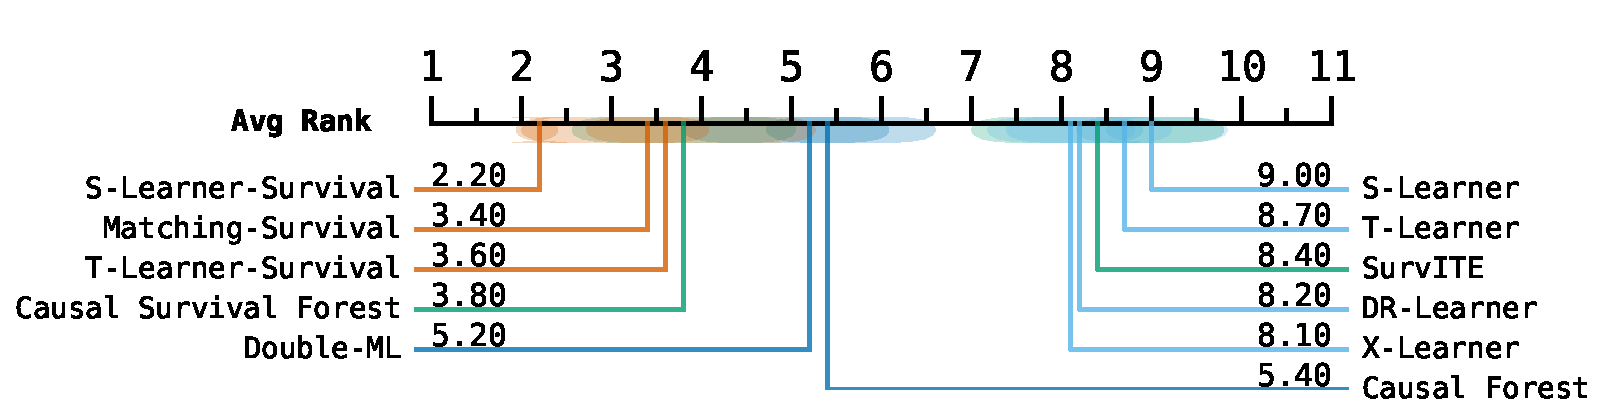
\includegraphics[width=\linewidth]{Appendices/appendix-ch04/images/figure_results_updated/average_ranks/average_ranking_visualization_method_combination_OBS-UConf-IC.pdf}
        \centering
        
        \label{ch04:fig:borda_ranking_causal_config_OBS_UConf_InfC}
    \end{minipage}}
    \hfill
    \subfloat[{RCT: \ChFourBlackCross, Ignorability: \ChFourGrayCheck, Positivity: \ChFourBlackCross, Ignorable Censoring: \ChFourBlackCross}]{\begin{minipage}[t]{0.49\textwidth}
        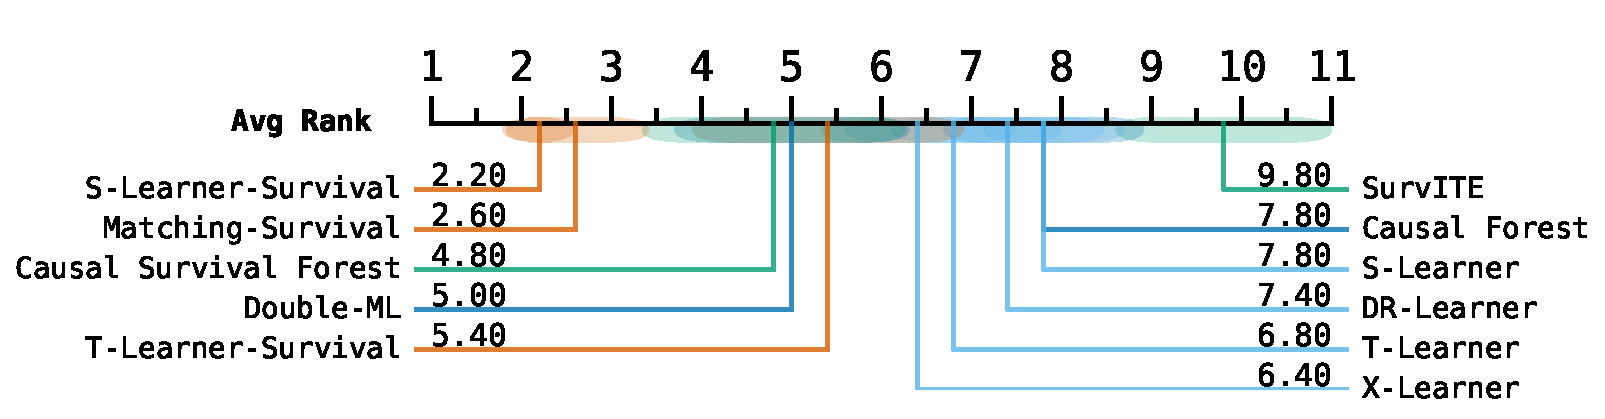
\includegraphics[width=\linewidth]{Appendices/appendix-ch04/images/figure_results_updated/average_ranks/average_ranking_visualization_method_combination_OBS-NoPos-IC.pdf}
        \centering
        
        \label{ch04:fig:borda_ranking_causal_config_OBS_NoPos_InfC}
    \end{minipage}}

    
    
}
\end{figure}



\ChFourRebuttal{In addition to the configuration-agnostic rankings in Figure~\ref{ch04:fig:average_rank_per_experiments}, we report win-rates by causal configuration in Tables~\ref{ch04:tab:winrate-rct-configs} and~\ref{ch04:tab:winrate-obs-configs}. For each configuration, we compute how often each method family appears in the Top-1, Top-3, and Top-5 positions for CATE RMSE and ATE Bias, aggregating over the five survival scenarios. This lets us separate the effect of causal assumptions (randomization, ignorability, positivity, and censoring) from the influence of the survival time model. The randomized settings (\texttt{RCT-50}, \texttt{RCT-5}) serve as our classical baselines, while the observational settings introduce unmeasured confounding, positivity violations, and informative censoring in a controlled way (Table~\ref{ch04:tab:synthetic-data-causal-config}).}

% \ChFourRebuttal{In the randomized configurations, outcome regression tends to perform well on CATE RMSE but is not uniformly dominant. Under \texttt{RCT-50}, Double-ML achieves the highest CATE RMSE win-rates (40.0 Top-1 and 80.0 Top-3/Top-5), with Causal Survival Forests and SurvITE also frequently appearing among the top methods. When treatment becomes sparse in \texttt{RCT-5}, Causal Survival Forests and Double-ML share the lead on CATE RMSE (Causal Survival Forests reaches 60.0 Top-1 and 80.0 Top-3/Top-5; Double-ML attains 20.0 Top-1 and 80.0 Top-5), while survival meta-learners such as S-Learner-Survival and Matching-Survival repeatedly enter the Top-3 and Top-5. Across both randomized settings, survival-specific approaches are already competitive on ATE Bias, with Causal Survival Forests, SurvITE, and several survival meta-learners appearing regularly among the top positions.}
\ChFourRebuttal{In the randomized configurations, CATE RMSE performance is split between outcome-imputation baselines and survival meta-learners, while ATE Bias results tend to favor survival-aware approaches. Under \texttt{RCT-50}, Double-ML, Causal Forest, Causal Survival Forests, T-Learner-Survival, and S-Learner-Survival all attain 20.0\% Top-1 on CATE RMSE, but the strongest Top-$k$ coverage comes from the survival meta-learners: S-Learner-Survival and Matching-Survival reach 100.0\% Top-5, and Matching-Survival achieves 60.0\% Top-3. For ATE Bias in \texttt{RCT-50}, S-Learner-Survival is the most frequent Top-1 method (40.0\%), with Causal Survival Forests and the survival meta-learners (including Matching-Survival and T-Learner-Survival) dominating Top-3/Top-5 (e.g., 60.0\% Top-3 for Causal Survival Forests and S-Learner-Survival; 80.0\% Top-5 for T-Learner-Survival, S-Learner-Survival, and Matching-Survival). When treatment assignment becomes sparse in \texttt{RCT-5}, Double-ML clearly leads on CATE RMSE (60.0\% Top-1 and 100.0\% Top-5), with Causal Survival Forests following (40.0\% Top-1; 60.0\% Top-3/Top-5). However, the ATE Bias rankings are largely driven by survival meta-learning: Matching-Survival achieves 40.0\% Top-1 and 80.0\% Top-3/Top-5, while S-Learner-Survival reaches 60.0\% Top-3/Top-5. Notably, SurvITE does not appear among the Top-$k$ in \texttt{RCT-5} and has only limited presence in \texttt{RCT-50}.}


% ============================
% RCT CONFIGURATIONS (GROUP 1)
% ============================

% !TeX root = ../../../main.tex
\begin{table}[htbp]
\ChFourFloatContents{ch04:tab:winrate-rct-configs}{\caption{\ChFourRebuttal{Win-rate (\%) of method families by Causal Configuration (randomized controlled trial settings). 
Values denote the percentage of times a method appears in the Top-1, Top-3, and Top-5 
according to CATE RMSE and ATE Bias across the five survival scenarios for each configuration.}}}{
\centering



\begin{minipage}{0.48\textwidth}
\centering
\textbf{\texttt{RCT-50}: 50\% treatment rate}\\[0.25em]
\begin{adjustbox}{max width=\textwidth}
\begin{tabular}{lccc@{\hspace{18pt}}ccc}
\toprule
\multirow{2}{*}{\textbf{Method Family}} &
\multicolumn{3}{c}{\textbf{CATE RMSE}} &
\multicolumn{3}{c}{\textbf{ATE Bias}} \\
\cmidrule(lr){2-4} \cmidrule(lr){5-7}
& \textbf{Top-1} & \textbf{Top-3} & \textbf{Top-5}
& \textbf{Top-1} & \textbf{Top-3} & \textbf{Top-5} \\
\midrule
\multicolumn{7}{l}{\textit{Outcome Imputation Methods}} \\
T-Learner               & \textcolor{gray}{0}   & \textcolor{gray}{0}   & 20.0 & \textcolor{gray}{0}   & 20.0 & 60.0 \\
S-Learner               & \textcolor{gray}{0}   & \textcolor{gray}{0}   & \textcolor{gray}{0}   & \textcolor{gray}{0}   & \textcolor{gray}{0}   & 20.0 \\
X-Learner               & \textcolor{gray}{0}   & \textcolor{gray}{0}   & 40.0 & 20.0 & 40.0 & 40.0 \\
DR-Learner              & \textcolor{gray}{0}   & \textcolor{gray}{0}   & \textcolor{gray}{0}   & \textcolor{gray}{0}   & 20.0 & 40.0 \\
Double-ML               & 20.0 & 60.0 & 80.0 & \textcolor{gray}{0}   & \textcolor{gray}{0}   & \textcolor{gray}{0} \\
Causal Forest           & 20.0 & 40.0 & 40.0 & \textcolor{gray}{0}   & \textcolor{gray}{0}   & 20.0 \\
\addlinespace %
\multicolumn{7}{l}{\textit{Direct-Survival CATE Methods}} \\
Causal Survival Forests  & 20.0 & 40.0 & 40.0 & 20.0 & 60.0 & 60.0 \\
SurvITE                 & \textcolor{gray}{0}   & \textcolor{gray}{0}   & 20.0 & \textcolor{gray}{0}   & 20.0 & 20.0 \\
\addlinespace %
\multicolumn{7}{l}{\textit{Survival Meta-Learners}} \\
T-Learner-Survival      & 20.0 & 40.0 & 60.0 & 20.0 & 40.0 & 80.0 \\
S-Learner-Survival      & 20.0 & 60.0 & 100.0 & 40.0 & 60.0 & 80.0 \\
Matching-Survival       & \textcolor{gray}{0}   & 60.0 & 100.0 & \textcolor{gray}{0}   & 40.0 & 80.0 \\
\bottomrule
\end{tabular}
\end{adjustbox}
\end{minipage}
\hfill
\begin{minipage}{0.48\textwidth}
\centering
\textbf{\texttt{RCT-5}: 5\% treatment rate}\\[0.25em]
\begin{adjustbox}{max width=\textwidth}
\begin{tabular}{lccc@{\hspace{18pt}}ccc}
\toprule
\multirow{2}{*}{\textbf{Method Family}} &
\multicolumn{3}{c}{\textbf{CATE RMSE}} &
\multicolumn{3}{c}{\textbf{ATE Bias}} \\
\cmidrule(lr){2-4} \cmidrule(lr){5-7}
& \textbf{Top-1} & \textbf{Top-3} & \textbf{Top-5}
& \textbf{Top-1} & \textbf{Top-3} & \textbf{Top-5} \\
\midrule
\multicolumn{7}{l}{\textit{Outcome Imputation Methods}} \\
T-Learner               & \textcolor{gray}{0}   & 20.0 & 60.0 & \textcolor{gray}{0}   & 20.0 & 60.0 \\
S-Learner               & \textcolor{gray}{0}   & 20.0 & 20.0 & 20.0 & 20.0 & 20.0 \\
X-Learner               & \textcolor{gray}{0}   & 20.0 & 60.0 & \textcolor{gray}{0}   & 20.0 & 60.0 \\
DR-Learner              & \textcolor{gray}{0}   & 20.0 & 40.0 & \textcolor{gray}{0}   & 20.0 & 60.0 \\
Double-ML               & 60.0 & 80.0 & 100.0 & 20.0 & 20.0 & 60.0 \\
Causal Forest           & \textcolor{gray}{0}   & \textcolor{gray}{0}   & 40.0 & \textcolor{gray}{0}   & 20.0 & 40.0 \\
\addlinespace %
\multicolumn{7}{l}{\textit{Direct-Survival CATE Methods}} \\
Causal Survival Forests  & 40.0 & 60.0 & 60.0 & 20.0 & 40.0 & 60.0 \\
SurvITE                 & \textcolor{gray}{0}   & \textcolor{gray}{0}   & \textcolor{gray}{0}   & \textcolor{gray}{0}   & \textcolor{gray}{0}   & \textcolor{gray}{0} \\
\addlinespace %
\multicolumn{7}{l}{\textit{Survival Meta-Learners}} \\
T-Learner-Survival      & \textcolor{gray}{0}   & 20.0 & 20.0 & \textcolor{gray}{0}   & \textcolor{gray}{0}   & \textcolor{gray}{0} \\
S-Learner-Survival      & \textcolor{gray}{0}   & 20.0 & 40.0 & \textcolor{gray}{0}   & 60.0 & 60.0 \\
Matching-Survival       & \textcolor{gray}{0}   & 40.0 & 60.0 & 40.0 & 80.0 & 80.0 \\
\bottomrule
\end{tabular}
\end{adjustbox}
\end{minipage}

}
\end{table}


% \ChFourRebuttal{The observational configurations highlight how violations of standard causal assumptions shift the balance further toward survival-focused methods. In \texttt{OBS-CPS} (no unmeasured confounding, no positivity or informative censoring), Double-ML and SurvITE are strong for CATE RMSE, but Causal Survival Forests and the survival meta-learners (especially S-Learner-Survival and Matching-Survival) capture most of the Top-1 and Top-3 spots for ATE Bias. Once unmeasured confounding is introduced (\texttt{OBS-UConf}), Causal Survival Forests, SurvITE, and the survival meta-learners dominate both metrics: Causal Survival Forests and Double-ML still perform well on CATE RMSE, but ATE Bias win-rates are almost entirely driven by Causal Survival Forests, SurvITE, S-Learner-Survival, and Matching-Survival. When positivity is violated (\texttt{OBS-NoPos}), Double-ML and SurvITE retain high CATE RMSE win-rates, whereas Causal Survival Forests and SurvITE achieve strong ATE Bias performance, and survival meta-learners again appear often in the Top-3 and Top-5.}
\ChFourRebuttal{The observational configurations further highlight how assumption violations shift performance toward survival-aware approaches, while revealing clear differences between \emph{direct-survival CATE} and \emph{survival meta-learner} families (Table~\ref{ch04:tab:winrate-obs-configs}). In \texttt{OBS-CPS} (no violations), CATE RMSE Top-1 is split across direct-survival CATE (Causal Survival Forests at 20.0\%) and Survival Meta-Learners (S-Learner-Survival and Matching-Survival at 20.0\% each), but the strongest Top-$k$ coverage comes from the Survival Meta-Learners: S-Learner-Survival and Matching-Survival reach 80.0\% Top-3 and 100.0\% Top-5. For ATE Bias in \texttt{OBS-CPS}, the lead is primarily driven by Survival Meta-Learners (S-Learner-Survival at 40.0\% Top-1; Matching-Survival at 80.0\% Top-3 and 100.0\% Top-5; T-Learner-Survival at 80.0\% Top-5), while the direct-survival CATE method Causal Survival Forests remains highly competitive in the upper ranks (60.0\% Top-3 and 80.0\% Top-5). Once unmeasured confounding is introduced (\texttt{OBS-UConf}), outcome imputation methods remain competitive for CATE RMSE (e.g., Double-ML at 20.0\% Top-1 and 80.0\% Top-5), but the top positions are shared with direct-survival CATE and Survival Meta-Learners (Causal Survival Forests, SurvITE, and S-Learner-Survival each at 20.0\% Top-1). For ATE Bias under \texttt{OBS-UConf}, direct-survival CATE takes the clearest lead at the very top (Causal Survival Forests at 40.0\% Top-1), while Survival Meta-Learners provide the strongest Top-3 presence (Matching-Survival at 60.0\% Top-3) and consistent Top-5 coverage (e.g., 60.0\% Top-5 for T-Learner-Survival, S-Learner-Survival, and Matching-Survival). Under positivity violations (\texttt{OBS-NoPos}), Outcome imputation dominates CATE RMSE Top-1 (Double-ML at 40.0\% and also T-Learner and X-Learner at 20.0\% each), whereas the Survival Meta-Learners remain highly competitive (S-Learner-Survival at 40.0\% Top-1 and 60.0\% Top-5; Matching-Survival at 80.0\% Top-5). In contrast, ATE Bias in \texttt{OBS-NoPos} is driven mainly by direct-survival CATE and Survival Meta-Learners: Causal Survival Forests reaches 80.0\% Top-3/Top-5, while Matching-Survival attains 40.0\% Top-1 coverage.}


% \ChFourRebuttal{Informative censoring amplifies these trends. In \texttt{OBS-CPS-InfC}, Causal Survival Forests, S-Learner-Survival, and Matching-Survival account for most of the Top-1 and Top-3 appearances for both CATE RMSE and ATE Bias, while Double-ML is mostly confined to Top-5 ranks. Under \texttt{OBS-UConf-InfC}, Causal Survival Forests becomes overwhelmingly dominant, reaching 80.0 Top-1 and 100.0 Top-3/Top-5 for CATE RMSE and similarly high win-rates for ATE Bias, with survival meta-learners providing additional support. Finally, in \texttt{OBS-NoPos-InfC}, Double-ML and Causal Survival Forests still perform well on CATE RMSE, but ATE Bias is largely controlled by Causal Survival Forests and the survival meta-learners, particularly T-Learner-Survival, S-Learner-Survival, and Matching-Survival. Overall, these patterns reinforce that direct survival modeling and survival meta-learning offer robustness as assumptions are progressively violated, especially when unmeasured confounding and informative censoring are present.}
\ChFourRebuttal{Informative censoring amplifies these differences and further separates the three method families. In \texttt{OBS-CPS-InfC}, CATE RMSE Top-1 is led by the direct-survival CATE family via Causal Survival Forests (40.0\%), while Survival Meta-Learners dominate Top-3/Top-5 coverage (S-Learner-Survival and Matching-Survival at 80.0\% Top-3 and 100.0\% Top-5). For ATE Bias in \texttt{OBS-CPS-InfC}, Survival Meta-Learners are the clear winners in the upper ranks (S-Learner-Survival at 100.0\% Top-3/Top-5; T-Learner-Survival at 40.0\% Top-1 and 80.0\% Top-5), with direct-survival CATE (Causal Survival Forests) still frequently among the top methods (80.0\% Top-5). Under \texttt{OBS-UConf-InfC}, CATE RMSE Top-1 is shared by direct-survival CATE (Causal Survival Forests at 40.0\%) and Survival Meta-Learners (T-Learner-Survival at 40.0\%), while Survival Meta-Learners dominate Top-3/Top-5 (S-Learner-Survival at 100.0\% Top-3/Top-5; Matching-Survival at 100.0\% Top-5). For ATE Bias in \texttt{OBS-UConf-InfC}, the strongest Top-1 signal comes from Survival Meta-Learners (T-Learner-Survival at 40.0\%), while direct-survival CATE shows the most dominant Top-5 presence (Causal Survival Forests at 100.0\% Top-5). Finally, in \texttt{OBS-NoPos-InfC}, Survival Meta-Learners clearly lead CATE RMSE (Matching-Survival at 40.0\% Top-1 and 100.0\% Top-5; S-Learner-Survival at 100.0\% Top-3/Top-5), whereas ATE Bias is again primarily driven by Survival Meta-Learners (T-Learner-Survival at 60.0\% Top-1 and 100.0\% Top-5), with direct-survival CATE remaining highly competitive in the upper ranks (Causal Survival Forests at 60.0\% Top-3 and 80.0\% Top-5). Overall, these patterns reinforce that as assumptions are progressively violated, Outcome imputation families can remain competitive for CATE RMSE in some regimes (notably \texttt{OBS-NoPos}), but direct-survival CATE and Survival Meta-Learners dominate the upper ranks for ATE Bias, especially under informative censoring and in settings with multiple simultaneous violations.}

% ================================
% OBSERVATIONAL CONFIGS (GROUP 2)
% ================================

% !TeX root = ../../../main.tex
\begin{table}[htbp]
\ChFourFloatContents{ch04:tab:winrate-obs-configs}{\caption{\ChFourRebuttal{Win-rate (\%) of method families by Causal Configuration (observational study settings). 
Values denote the percentage of times a method appears in the Top-1, Top-3, and Top-5 according to CATE RMSE and ATE Bias across the five survival scenarios for each configuration. }}}{
\centering



\begin{minipage}{0.48\textwidth}
\centering
\textbf{\texttt{OBS-CPS}}\\[0.25em]
\begin{adjustbox}{max width=\textwidth}
\begin{tabular}{lccc@{\hspace{18pt}}ccc}
\toprule
\multirow{2}{*}{\textbf{Method Family}} &
\multicolumn{3}{c}{\textbf{CATE RMSE}} &
\multicolumn{3}{c}{\textbf{ATE Bias}} \\
\cmidrule(lr){2-4} \cmidrule(lr){5-7}
& \textbf{Top-1} & \textbf{Top-3} & \textbf{Top-5}
& \textbf{Top-1} & \textbf{Top-3} & \textbf{Top-5} \\
\midrule
\multicolumn{7}{l}{\textit{Outcome Imputation Methods}} \\
T-Learner               & \textcolor{gray}{0}   & \textcolor{gray}{0}   & 40.0 & \textcolor{gray}{0}   & \textcolor{gray}{0}   & 20.0 \\
S-Learner               & \textcolor{gray}{0}   & \textcolor{gray}{0}   & \textcolor{gray}{0}   & \textcolor{gray}{0}   & \textcolor{gray}{0}   & 20.0 \\
X-Learner               & \textcolor{gray}{0}   & \textcolor{gray}{0}   & 20.0 & \textcolor{gray}{0}   & 20.0 & 20.0 \\
DR-Learner              & \textcolor{gray}{0}   & 20.0 & 20.0 & \textcolor{gray}{0}   & \textcolor{gray}{0}   & \textcolor{gray}{0} \\
Double-ML               & 20.0 & 40.0 & 80.0 & \textcolor{gray}{0}   & \textcolor{gray}{0}   & \textcolor{gray}{0} \\
Causal Forest           & 20.0 & 20.0 & 40.0 & \textcolor{gray}{0}   & 20.0 & 20.0 \\
\addlinespace %
\multicolumn{7}{l}{\textit{Direct-Survival CATE Methods}} \\
Causal Survival Forests  & 20.0 & 40.0 & 60.0 & \textcolor{gray}{0}   & 60.0 & 80.0 \\
SurvITE                 & \textcolor{gray}{0}   & \textcolor{gray}{0}   & 20.0 & 20.0 & 20.0 & 60.0 \\
\addlinespace %
\multicolumn{7}{l}{\textit{Survival Meta-Learners}} \\
T-Learner-Survival      & \textcolor{gray}{0}   & 20.0 & 20.0 & 20.0 & 40.0 & 80.0 \\
S-Learner-Survival      & 20.0 & 80.0 & 100.0 & 40.0 & 60.0 & 100.0 \\
Matching-Survival       & 20.0 & 80.0 & 100.0 & 20.0 & 80.0 & 100.0 \\
\bottomrule
\end{tabular}
\end{adjustbox}
\end{minipage}
\hfill
\begin{minipage}{0.48\textwidth}
\centering
\textbf{\texttt{OBS-UConf}}\\[0.25em]
\begin{adjustbox}{max width=\textwidth}
\begin{tabular}{lccc@{\hspace{18pt}}ccc}
\toprule
\multirow{2}{*}{\textbf{Method Family}} &
\multicolumn{3}{c}{\textbf{CATE RMSE}} &
\multicolumn{3}{c}{\textbf{ATE Bias}} \\
\cmidrule(lr){2-4} \cmidrule(lr){5-7}
& \textbf{Top-1} & \textbf{Top-3} & \textbf{Top-5}
& \textbf{Top-1} & \textbf{Top-3} & \textbf{Top-5} \\
\midrule
\multicolumn{7}{l}{\textit{Outcome Imputation Methods}} \\
T-Learner               & \textcolor{gray}{0}   & 20.0 & 20.0 & \textcolor{gray}{0}   & 20.0 & 40.0 \\
S-Learner               & \textcolor{gray}{0}   & \textcolor{gray}{0}   & \textcolor{gray}{0}   & \textcolor{gray}{0}   & 40.0 & 40.0 \\
X-Learner               & \textcolor{gray}{0}   & 20.0 & 40.0 & \textcolor{gray}{0}   & \textcolor{gray}{0}   & 60.0 \\
DR-Learner              & \textcolor{gray}{0}   & \textcolor{gray}{0}   & 20.0 & 20.0 & 40.0 & 40.0 \\
Double-ML               & 20.0 & 60.0 & 80.0 & \textcolor{gray}{0}   & \textcolor{gray}{0}   & 20.0 \\
Causal Forest           & 20.0 & 40.0 & 40.0 & \textcolor{gray}{0}   & \textcolor{gray}{0}   & 20.0 \\
\addlinespace %
\multicolumn{7}{l}{\textit{Direct-Survival CATE Methods}} \\
Causal Survival Forests  & 20.0 & 40.0 & 60.0 & 40.0 & 60.0 & 60.0 \\
SurvITE                 & 20.0 & 20.0 & 40.0 & 20.0 & 40.0 & 40.0 \\
\addlinespace %
\multicolumn{7}{l}{\textit{Survival Meta-Learners}} \\
T-Learner-Survival      & \textcolor{gray}{0}   & 20.0 & 20.0 & \textcolor{gray}{0}   & \textcolor{gray}{0}   & 60.0 \\
S-Learner-Survival      & 20.0 & 60.0 & 80.0 & \textcolor{gray}{0}   & 40.0 & 60.0 \\
Matching-Survival       & \textcolor{gray}{0}   & 20.0 & 100.0 & 20.0 & 60.0 & 60.0 \\
\bottomrule
\end{tabular}
\end{adjustbox}
\end{minipage}



\begin{minipage}{0.48\textwidth}
\centering
\textbf{\texttt{OBS-NoPos}}\\[0.25em]
\begin{adjustbox}{max width=\textwidth}
\begin{tabular}{lccc@{\hspace{18pt}}ccc}
\toprule
\multirow{2}{*}{\textbf{Method Family}} &
\multicolumn{3}{c}{\textbf{CATE RMSE}} &
\multicolumn{3}{c}{\textbf{ATE Bias}} \\
\cmidrule(lr){2-4} \cmidrule(lr){5-7}
& \textbf{Top-1} & \textbf{Top-3} & \textbf{Top-5}
& \textbf{Top-1} & \textbf{Top-3} & \textbf{Top-5} \\
\midrule
\multicolumn{7}{l}{\textit{Outcome Imputation Methods}} \\
T-Learner               & 20.0 & 40.0 & 60.0 & \textcolor{gray}{0}   & 20.0 & 40.0 \\
S-Learner               & \textcolor{gray}{0}   & \textcolor{gray}{0}   & \textcolor{gray}{0}   & \textcolor{gray}{0}   & 40.0 & 60.0 \\
X-Learner               & 20.0 & 40.0 & 80.0 & \textcolor{gray}{0}   & 20.0 & 60.0 \\
DR-Learner              & \textcolor{gray}{0}   & 20.0 & 20.0 & \textcolor{gray}{0}   & \textcolor{gray}{0}   & 40.0 \\
Double-ML               & 40.0 & 60.0 & 60.0 & \textcolor{gray}{0}   & 20.0 & 20.0 \\
Causal Forest           & \textcolor{gray}{0}   & 20.0 & 40.0 & 20.0 & 20.0 & 20.0 \\
\addlinespace %
\multicolumn{7}{l}{\textit{Direct-Survival CATE Methods}} \\
Causal Survival Forests  & \textcolor{gray}{0}   & 40.0 & 40.0 & 20.0 & 80.0 & 80.0 \\
SurvITE                 & \textcolor{gray}{0}   & 20.0 & 40.0 & \textcolor{gray}{0}   & 20.0 & 40.0 \\
\addlinespace %
\multicolumn{7}{l}{\textit{Survival Meta-Learners}} \\
T-Learner-Survival      & \textcolor{gray}{0}   & 20.0 & 20.0 & 20.0 & 20.0 & 20.0 \\
S-Learner-Survival      & 40.0 & 40.0 & 60.0 & \textcolor{gray}{0}   & 20.0 & 80.0 \\
Matching-Survival       & \textcolor{gray}{0}   & 20.0 & 80.0 & 40.0 & 40.0 & 40.0 \\
\bottomrule
\end{tabular}
\end{adjustbox}
\end{minipage}
\hfill
\begin{minipage}{0.48\textwidth}
\centering
\textbf{\texttt{OBS-CPS-InfC}}\\[0.25em]
\begin{adjustbox}{max width=\textwidth}
\begin{tabular}{lccc@{\hspace{18pt}}ccc}
\toprule
\multirow{2}{*}{\textbf{Method Family}} &
\multicolumn{3}{c}{\textbf{CATE RMSE}} &
\multicolumn{3}{c}{\textbf{ATE Bias}} \\
\cmidrule(lr){2-4} \cmidrule(lr){5-7}
& \textbf{Top-1} & \textbf{Top-3} & \textbf{Top-5}
& \textbf{Top-1} & \textbf{Top-3} & \textbf{Top-5} \\
\midrule
\multicolumn{7}{l}{\textit{Outcome Imputation Methods}} \\
T-Learner               & \textcolor{gray}{0}   & \textcolor{gray}{0}   & \textcolor{gray}{0}   & \textcolor{gray}{0}   & \textcolor{gray}{0}   & \textcolor{gray}{0} \\
S-Learner               & \textcolor{gray}{0}   & \textcolor{gray}{0}   & \textcolor{gray}{0}   & \textcolor{gray}{0}   & \textcolor{gray}{0}   & \textcolor{gray}{0} \\
X-Learner               & \textcolor{gray}{0}   & \textcolor{gray}{0}   & \textcolor{gray}{0}   & \textcolor{gray}{0}   & \textcolor{gray}{0}   & 40.0 \\
DR-Learner              & \textcolor{gray}{0}   & \textcolor{gray}{0}   & 40.0 & 20.0 & 20.0 & 20.0 \\
Double-ML               & \textcolor{gray}{0}   & 40.0 & 60.0 & \textcolor{gray}{0}   & \textcolor{gray}{0}   & \textcolor{gray}{0} \\
Causal Forest           & \textcolor{gray}{0}   & 20.0 & 60.0 & \textcolor{gray}{0}   & \textcolor{gray}{0}   & 40.0 \\
\addlinespace %
\multicolumn{7}{l}{\textit{Direct-Survival CATE Methods}} \\
Causal Survival Forests  & 40.0 & 60.0 & 60.0 & 20.0 & 40.0 & 80.0 \\
SurvITE                 & \textcolor{gray}{0}   & \textcolor{gray}{0}   & \textcolor{gray}{0}   & 20.0 & 20.0 & 60.0 \\
\addlinespace %
\multicolumn{7}{l}{\textit{Survival Meta-Learners}} \\
T-Learner-Survival      & 20.0 & 20.0 & 80.0 & 40.0 & 60.0 & 80.0 \\
S-Learner-Survival      & 20.0 & 80.0 & 100.0 & \textcolor{gray}{0}   & 100.0 & 100.0 \\
Matching-Survival       & 20.0 & 80.0 & 100.0 & \textcolor{gray}{0}   & 60.0 & 80.0 \\
\bottomrule
\end{tabular}
\end{adjustbox}
\end{minipage}



\begin{minipage}{0.48\textwidth}
\centering
\textbf{\texttt{OBS-UConf-InfC}}\\[0.25em]
\begin{adjustbox}{max width=\textwidth}
\begin{tabular}{lccc@{\hspace{18pt}}ccc}
\toprule
\multirow{2}{*}{\textbf{Method Family}} &
\multicolumn{3}{c}{\textbf{CATE RMSE}} &
\multicolumn{3}{c}{\textbf{ATE Bias}} \\
\cmidrule(lr){2-4} \cmidrule(lr){5-7}
& \textbf{Top-1} & \textbf{Top-3} & \textbf{Top-5}
& \textbf{Top-1} & \textbf{Top-3} & \textbf{Top-5} \\
\midrule
\multicolumn{7}{l}{\textit{Outcome Imputation Methods}} \\
T-Learner               & \textcolor{gray}{0}   & \textcolor{gray}{0}   & \textcolor{gray}{0}   & \textcolor{gray}{0}   & 20.0 & 20.0 \\
S-Learner               & \textcolor{gray}{0}   & \textcolor{gray}{0}   & \textcolor{gray}{0}   & 20.0 & 20.0 & 20.0 \\
X-Learner               & \textcolor{gray}{0}   & \textcolor{gray}{0}   & \textcolor{gray}{0}   & \textcolor{gray}{0}   & 20.0 & 20.0 \\
DR-Learner              & \textcolor{gray}{0}   & \textcolor{gray}{0}   & \textcolor{gray}{0}   & \textcolor{gray}{0}   & \textcolor{gray}{0}   & 20.0 \\
Double-ML               & \textcolor{gray}{0}   & 40.0 & 60.0 & \textcolor{gray}{0}   & \textcolor{gray}{0}   & 20.0 \\
Causal Forest           & \textcolor{gray}{0}   & \textcolor{gray}{0}   & 60.0 & \textcolor{gray}{0}   & \textcolor{gray}{0}   & 20.0 \\
\addlinespace %
\multicolumn{7}{l}{\textit{Direct-Survival CATE Methods}} \\
Causal Survival Forests  & 40.0 & 40.0 & 60.0 & \textcolor{gray}{0}   & 20.0 & 100.0 \\
SurvITE                 & \textcolor{gray}{0}   & \textcolor{gray}{0}   & 40.0 & \textcolor{gray}{0}   & 20.0 & 40.0 \\
\addlinespace %
\multicolumn{7}{l}{\textit{Survival Meta-Learners}} \\
T-Learner-Survival      & 40.0 & 80.0 & 80.0 & 40.0 & 60.0 & 80.0 \\
S-Learner-Survival      & \textcolor{gray}{0}   & 100.0 & 100.0 & 20.0 & 80.0 & 80.0 \\
Matching-Survival       & 20.0 & 40.0 & 100.0 & 20.0 & 60.0 & 80.0 \\
\bottomrule
\end{tabular}
\end{adjustbox}
\end{minipage}
\hfill
\begin{minipage}{0.48\textwidth}
\centering
\textbf{\texttt{OBS-NoPos-InfC}}\\[0.25em]
\begin{adjustbox}{max width=\textwidth}
\begin{tabular}{lccc@{\hspace{18pt}}ccc}
\toprule
\multirow{2}{*}{\textbf{Method Family}} &
\multicolumn{3}{c}{\textbf{CATE RMSE}} &
\multicolumn{3}{c}{\textbf{ATE Bias}} \\
\cmidrule(lr){2-4} \cmidrule(lr){5-7}
& \textbf{Top-1} & \textbf{Top-3} & \textbf{Top-5}
& \textbf{Top-1} & \textbf{Top-3} & \textbf{Top-5} \\
\midrule
\multicolumn{7}{l}{\textit{Outcome Imputation Methods}} \\
T-Learner               & \textcolor{gray}{0}   & 20.0 & 40.0 & 20.0 & 20.0 & 20.0 \\
S-Learner               & \textcolor{gray}{0}   & \textcolor{gray}{0}   & \textcolor{gray}{0}   & \textcolor{gray}{0}   & \textcolor{gray}{0}   & 20.0 \\
X-Learner               & \textcolor{gray}{0}   & 20.0 & 40.0 & 20.0 & 20.0 & 20.0 \\
DR-Learner              & \textcolor{gray}{0}   & \textcolor{gray}{0}   & 40.0 & \textcolor{gray}{0}   & \textcolor{gray}{0}   & 20.0 \\
Double-ML               & \textcolor{gray}{0}   & 40.0 & 60.0 & \textcolor{gray}{0}   & \textcolor{gray}{0}   & 20.0 \\
Causal Forest           & \textcolor{gray}{0}   & \textcolor{gray}{0}   & 20.0 & \textcolor{gray}{0}   & \textcolor{gray}{0}   & 40.0 \\
\addlinespace %
\multicolumn{7}{l}{\textit{Direct-Survival CATE Methods}} \\
Causal Survival Forests  & 20.0 & 40.0 & 40.0 & 20.0 & 60.0 & 80.0 \\
SurvITE                 & \textcolor{gray}{0}   & \textcolor{gray}{0}   & 20.0 & \textcolor{gray}{0}   & 40.0 & 60.0 \\
\addlinespace %
\multicolumn{7}{l}{\textit{Survival Meta-Learners}} \\
T-Learner-Survival      & 20.0 & 40.0 & 40.0 & 60.0 & 80.0 & 100.0 \\
S-Learner-Survival      & 20.0 & 100.0 & 100.0 & \textcolor{gray}{0}   & 40.0 & 60.0 \\
Matching-Survival       & 40.0 & 60.0 & 100.0 & \textcolor{gray}{0}   & 40.0 & 60.0 \\
\bottomrule
\end{tabular}
\end{adjustbox}
\end{minipage}

}
\end{table}




%%%%%%%%%%%%%%%%%%%%%%%%%%%%%%%%%%%%%%%%%%%%%%%%%%%%%%%%%%%%%%%%
%%%%%%%%%%%%%%%%%%%%%%%%%%%%%%%%%%%%%%%%%%%%%%%%%%%%%%%%%%%%%%%%
%%%%%%%%%%%%%%%%%%%%%%%%%%%%%%%%%%%%%%%%%%%%%%%%

\subsubsection{Figure results - CATE RMSE} \label{ch04:app:more-cate-mse-plots}

This section presents the complete CATE RMSE results for each family of causal inference methods across various survival analysis scenarios.
For each scenario, we display performance under 8 distinct causal configurations, each varying in terms of treatment assignment (RCT vs. observational), ignorability, positivity, and censoring assumptions.
These results highlight the robustness and sensitivity of different methods under varying degrees of assumption violations.

For each survival scenario and causal configuration, we selected the best hyperparameter setting and base model configuration for each causal method family based on validation set performance.
The RMSE values shown in the figures reflect the performance of these selected models on the test set.
The box plots are from the 10 independent experimental repeats to account for random seed variability.



% Secnario A

% !TeX root = ../../../main.tex
\begin{figure}[htbp]
\ChFourFloatContents{ch04:fig:cate_mse_grid_scenario_A}{\caption{CATE RMSE across different experiments in Scenario \texttt{A}.}}{
    \centering

    \resizebox{0.95\textwidth}{!}{%
        \begin{minipage}{1\textwidth}


    \subfloat[{RCT: \ChFourGrayCheck (50\%), Ignorability: \ChFourGrayCheck, Positivity: \ChFourGrayCheck, Ign-Censoring: \ChFourGrayCheck}]{\begin{minipage}[t]{0.49\textwidth}
        \centering
        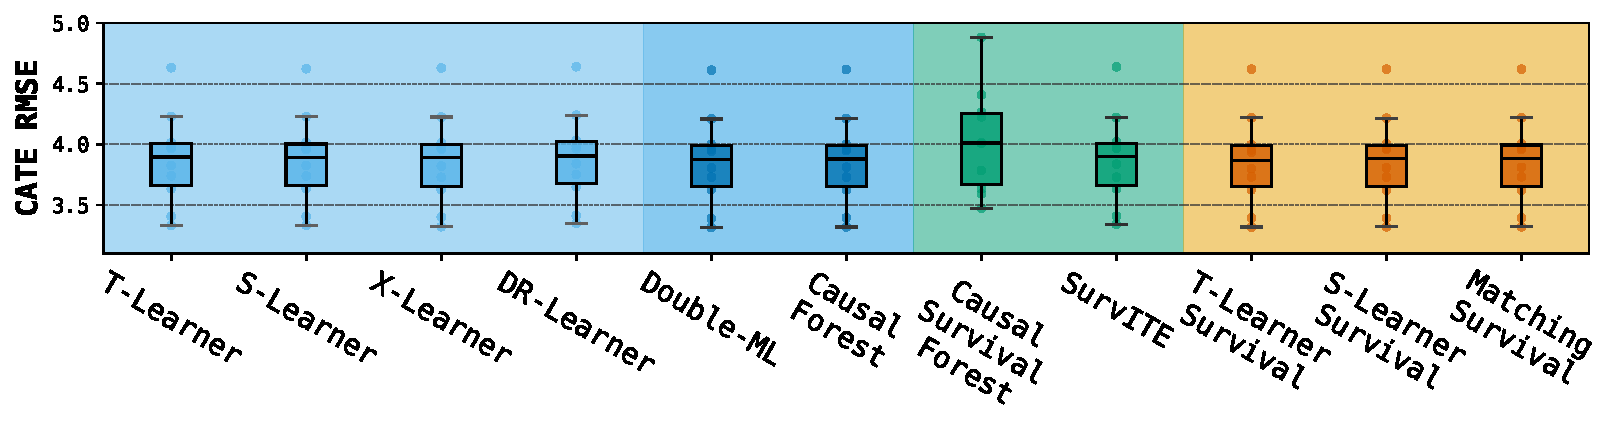
\includegraphics[width=\linewidth]{Appendices/appendix-ch04/images/figure_results_updated/cate_rmse/Scenario_A_RCT-50_cate_mse.pdf}
        
    \end{minipage}}
    \hfill
    \subfloat[{RCT: \ChFourGrayCheck (5\%), Ignorability: \ChFourGrayCheck, Positivity: \ChFourGrayCheck, Ign-Censoring: \ChFourGrayCheck}]{\begin{minipage}[t]{0.49\textwidth}
        \centering
        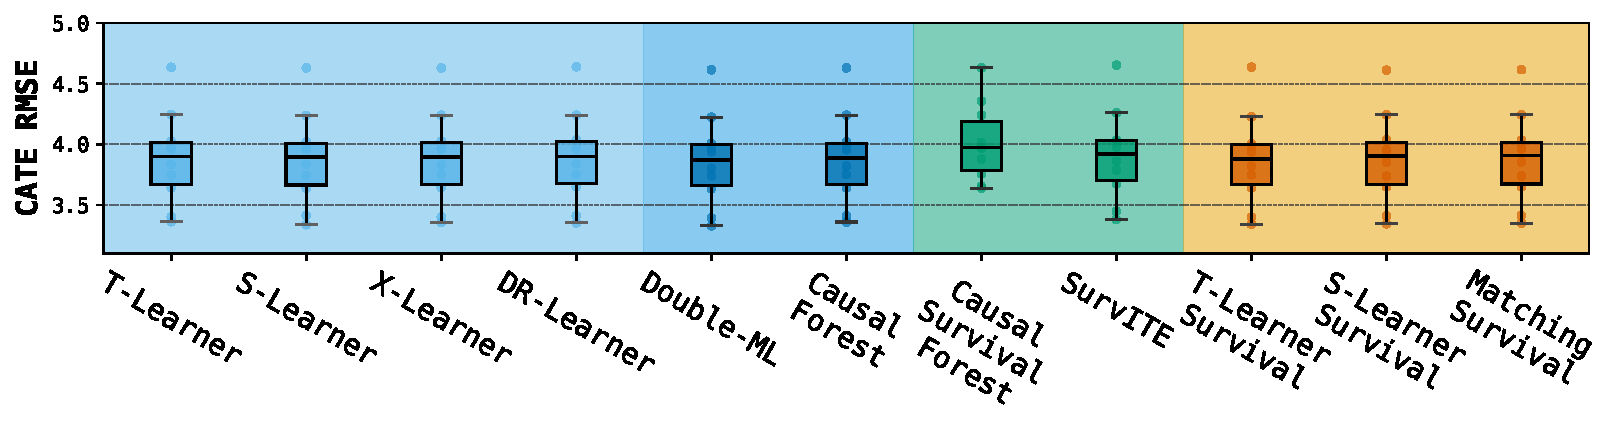
\includegraphics[width=\linewidth]{Appendices/appendix-ch04/images/figure_results_updated/cate_rmse/Scenario_A_RCT-5_cate_mse.pdf}
        
    \end{minipage}}

    

    \subfloat[{RCT: \ChFourBlackCross, Ignorability: \ChFourGrayCheck, Positivity: \ChFourGrayCheck, Ignorable Censoring: \ChFourGrayCheck}]{\begin{minipage}[t]{0.49\textwidth}
        \centering
        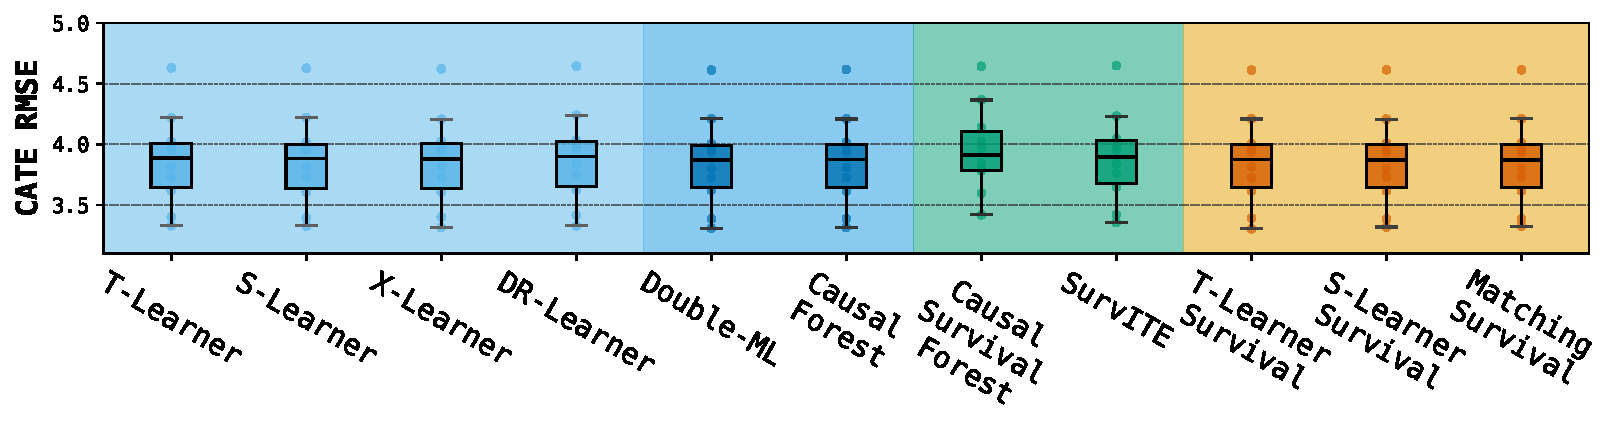
\includegraphics[width=\linewidth]{Appendices/appendix-ch04/images/figure_results_updated/cate_rmse/Scenario_A_OBS-CPS_cate_mse.pdf}
        
    \end{minipage}}
    \hfill
    \subfloat[{RCT: \ChFourBlackCross, Ignorability: \ChFourBlackCross, Positivity: \ChFourGrayCheck, Ignorable Censoring: \ChFourGrayCheck}]{\begin{minipage}[t]{0.49\textwidth}
        \centering
        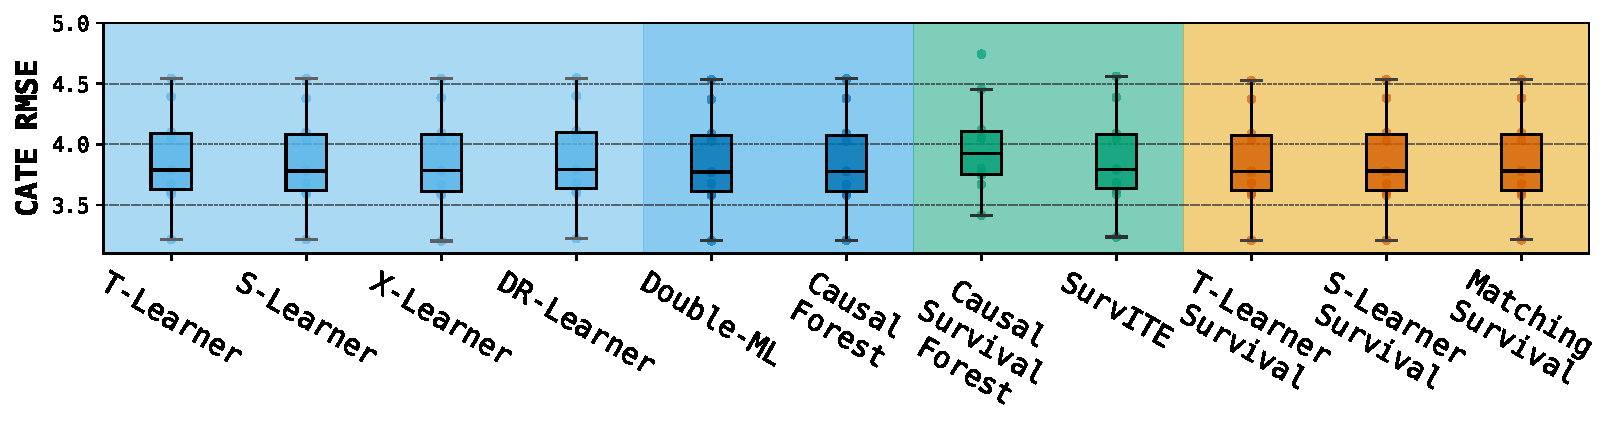
\includegraphics[width=\linewidth]{Appendices/appendix-ch04/images/figure_results_updated/cate_rmse/Scenario_A_OBS-UConf_cate_mse.pdf}
        
    \end{minipage}}

    

    \subfloat[{RCT: \ChFourBlackCross, Ignorability: \ChFourGrayCheck, Positivity: \ChFourBlackCross, Ignorable Censoring: \ChFourGrayCheck}]{\begin{minipage}[t]{0.49\textwidth}
        \centering
        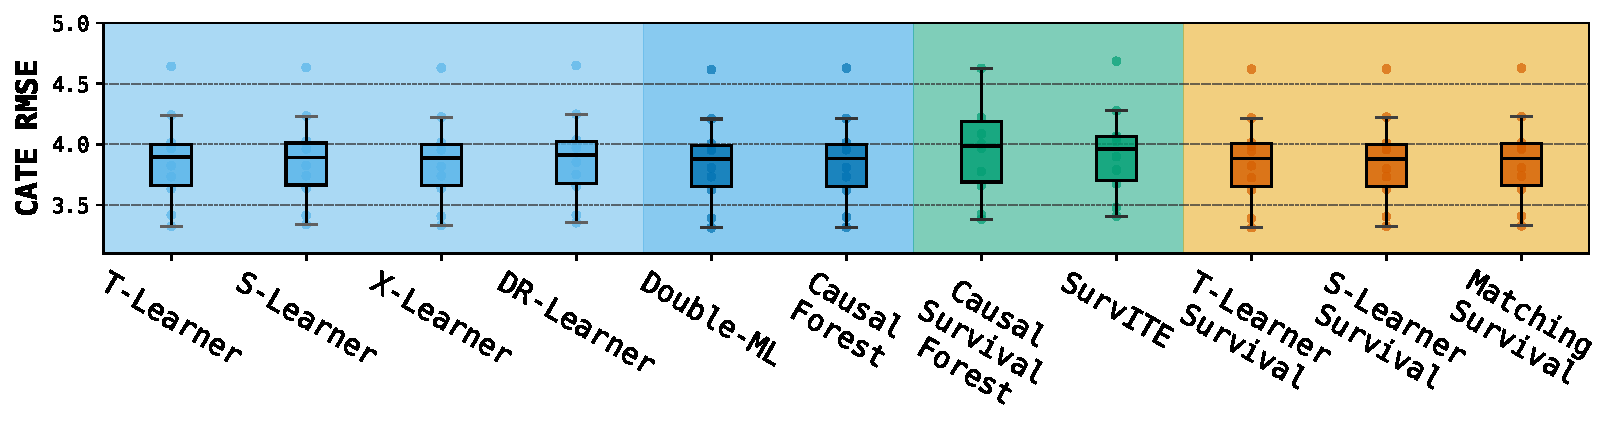
\includegraphics[width=\linewidth]{Appendices/appendix-ch04/images/figure_results_updated/cate_rmse/Scenario_A_OBS-NoPos_cate_mse.pdf}
        
    \end{minipage}}
    \hfill
    \subfloat[{RCT: \ChFourBlackCross, Ignorability: \ChFourGrayCheck, Positivity: \ChFourGrayCheck, Ignorable Censoring: \ChFourBlackCross}]{\begin{minipage}[t]{0.49\textwidth}
        \centering
        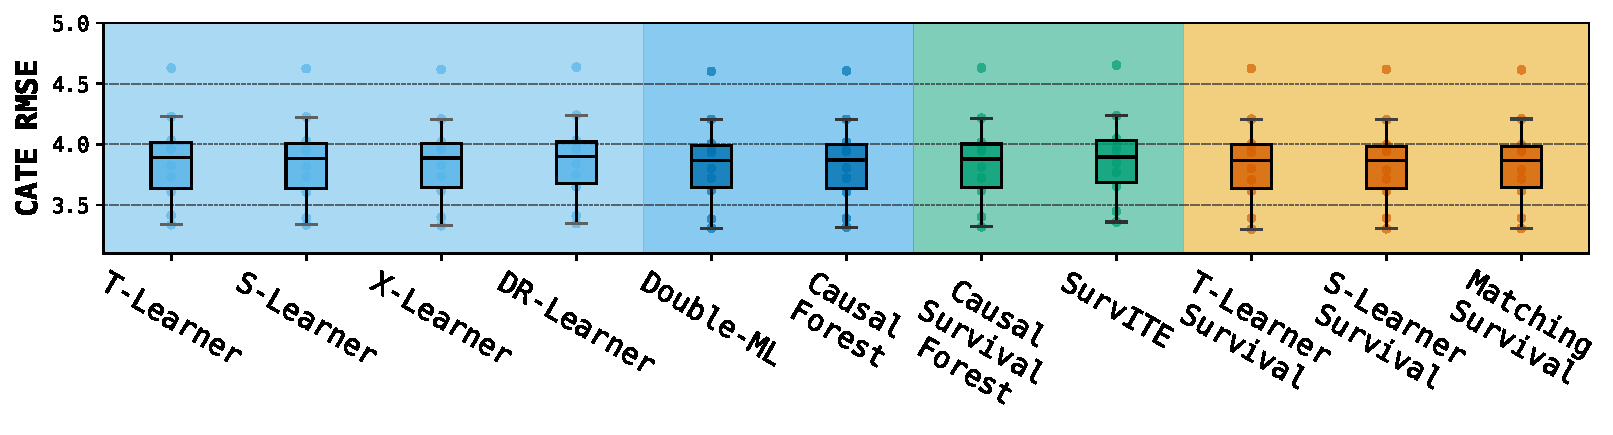
\includegraphics[width=\linewidth]{Appendices/appendix-ch04/images/figure_results_updated/cate_rmse/Scenario_A_OBS-CPS-IC_cate_mse.pdf}
        
    \end{minipage}}

    

    \subfloat[{RCT: \ChFourBlackCross, Ignorability: \ChFourBlackCross, Positivity: \ChFourGrayCheck, Ignorable Censoring: \ChFourBlackCross}]{\begin{minipage}[t]{0.49\textwidth}
        \centering
        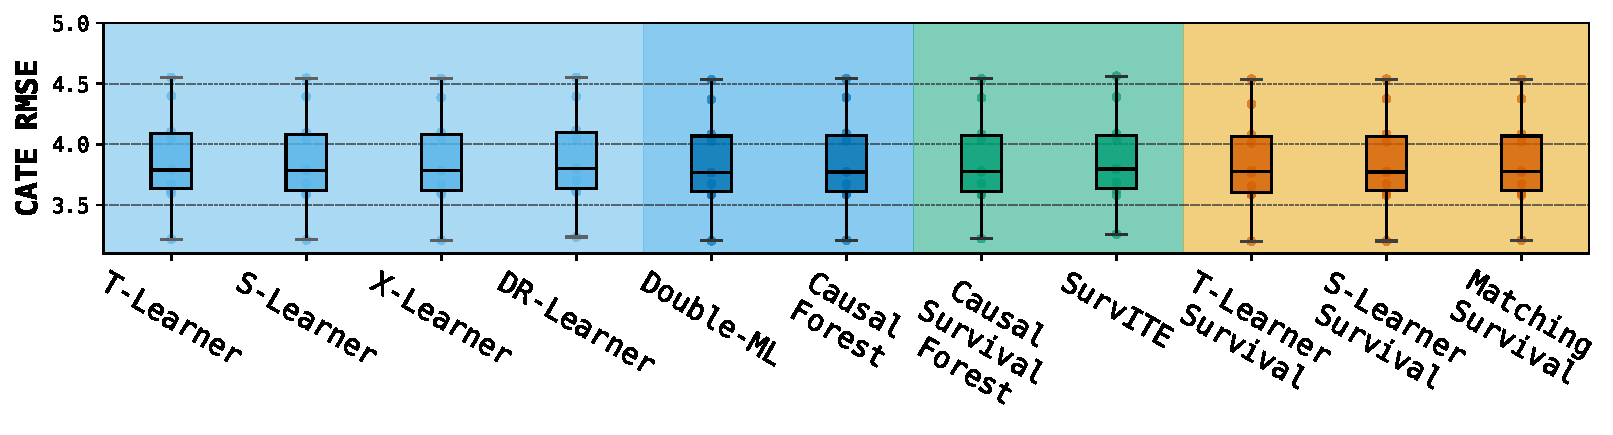
\includegraphics[width=\linewidth]{Appendices/appendix-ch04/images/figure_results_updated/cate_rmse/Scenario_A_OBS-UConf-IC_cate_mse.pdf}
        
    \end{minipage}}
    \hfill
    \subfloat[{RCT: \ChFourBlackCross, Ignorability: \ChFourGrayCheck, Positivity: \ChFourBlackCross, Ignorable Censoring: \ChFourBlackCross}]{\begin{minipage}[t]{0.49\textwidth}
        \centering
        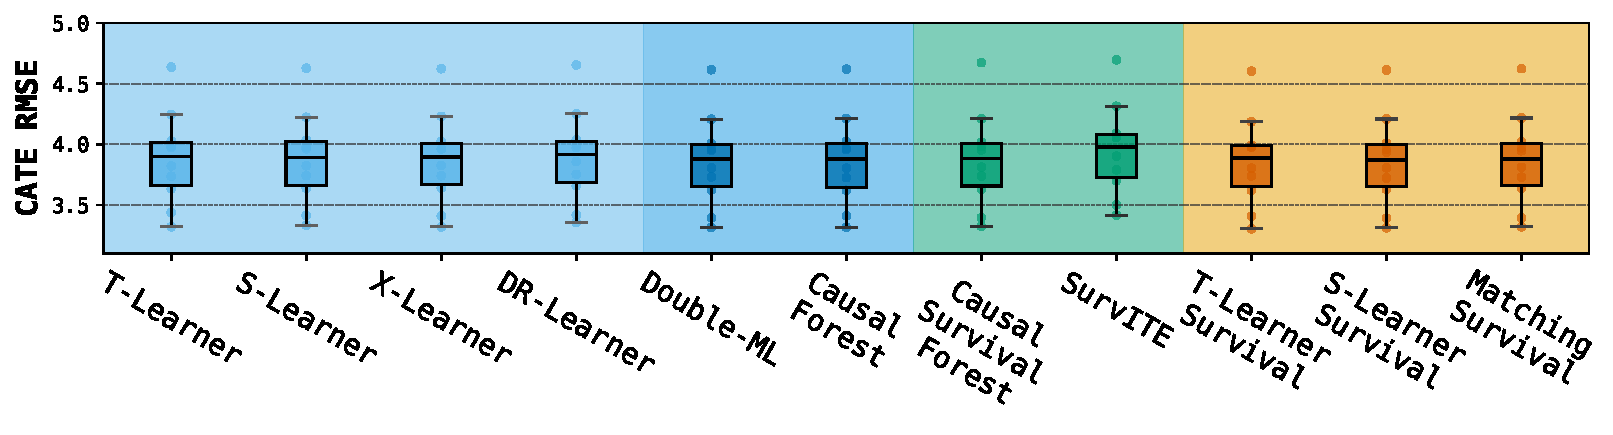
\includegraphics[width=\linewidth]{Appendices/appendix-ch04/images/figure_results_updated/cate_rmse/Scenario_A_OBS-NoPos-IC_cate_mse.pdf}
        
    \end{minipage}}

            \end{minipage}%
    }
    

    
    
}
\end{figure}


% Secnario B

% !TeX root = ../../../main.tex
\begin{figure}[htbp]
\ChFourFloatContents{ch04:fig:cate_mse_grid_scenario_B}{\caption{CATE RMSE across different experiments in Scenario \texttt{B}.}}{
    \centering

    \resizebox{0.95\textwidth}{!}{%
        \begin{minipage}{1\textwidth}


    \subfloat[{RCT: \ChFourGrayCheck (50\%), Ignorability: \ChFourGrayCheck, Positivity: \ChFourGrayCheck, Ign-Censoring: \ChFourGrayCheck}]{\begin{minipage}[t]{0.49\textwidth}
        \centering
        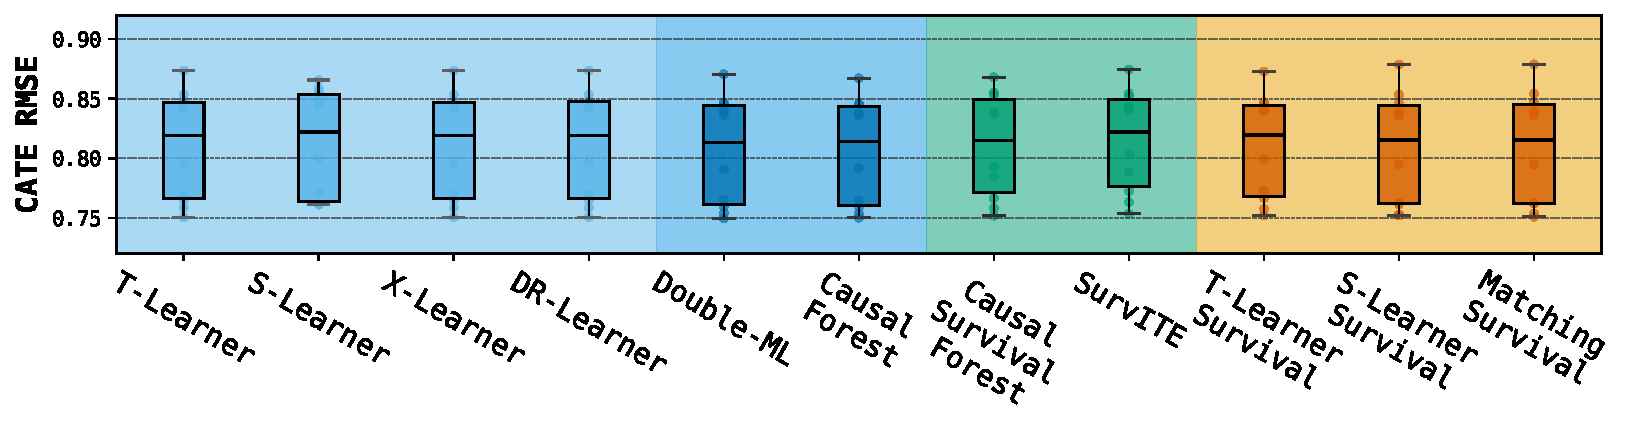
\includegraphics[width=\linewidth]{Appendices/appendix-ch04/images/figure_results_updated/cate_rmse/Scenario_B_RCT-50_cate_mse.pdf}
        
    \end{minipage}}
    \hfill
    \subfloat[{RCT: \ChFourGrayCheck (5\%), Ignorability: \ChFourGrayCheck, Positivity: \ChFourGrayCheck, Ign-Censoring: \ChFourGrayCheck}]{\begin{minipage}[t]{0.49\textwidth}
        \centering
        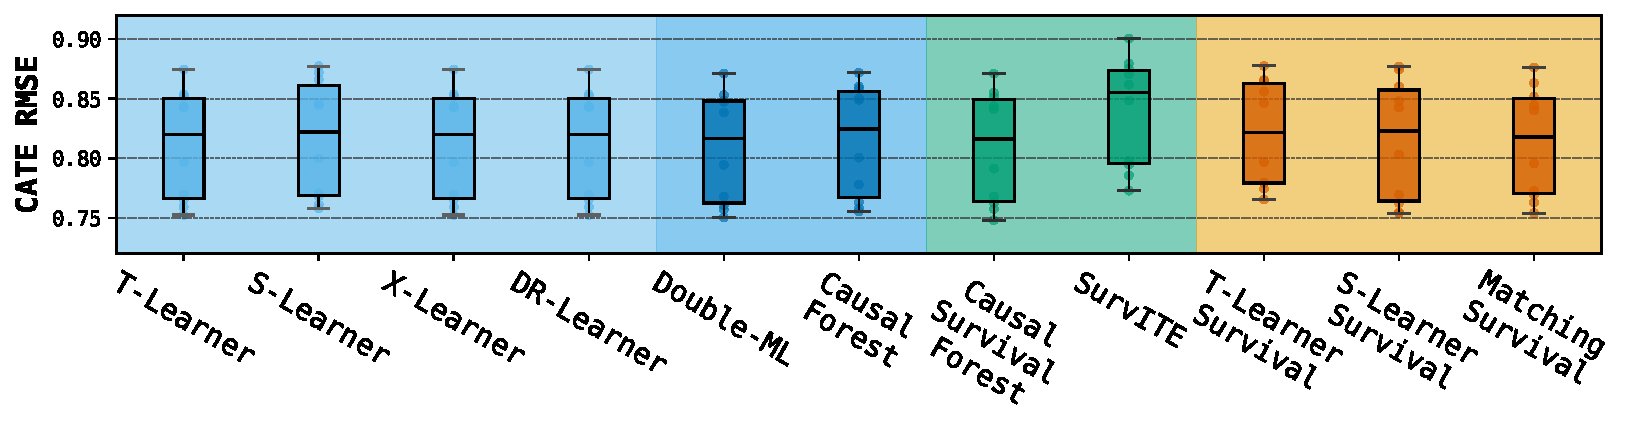
\includegraphics[width=\linewidth]{Appendices/appendix-ch04/images/figure_results_updated/cate_rmse/Scenario_B_RCT-5_cate_mse.pdf}
        
    \end{minipage}}

    

    \subfloat[{RCT: \ChFourBlackCross, Ignorability: \ChFourGrayCheck, Positivity: \ChFourGrayCheck, Ignorable Censoring: \ChFourGrayCheck}]{\begin{minipage}[t]{0.49\textwidth}
        \centering
        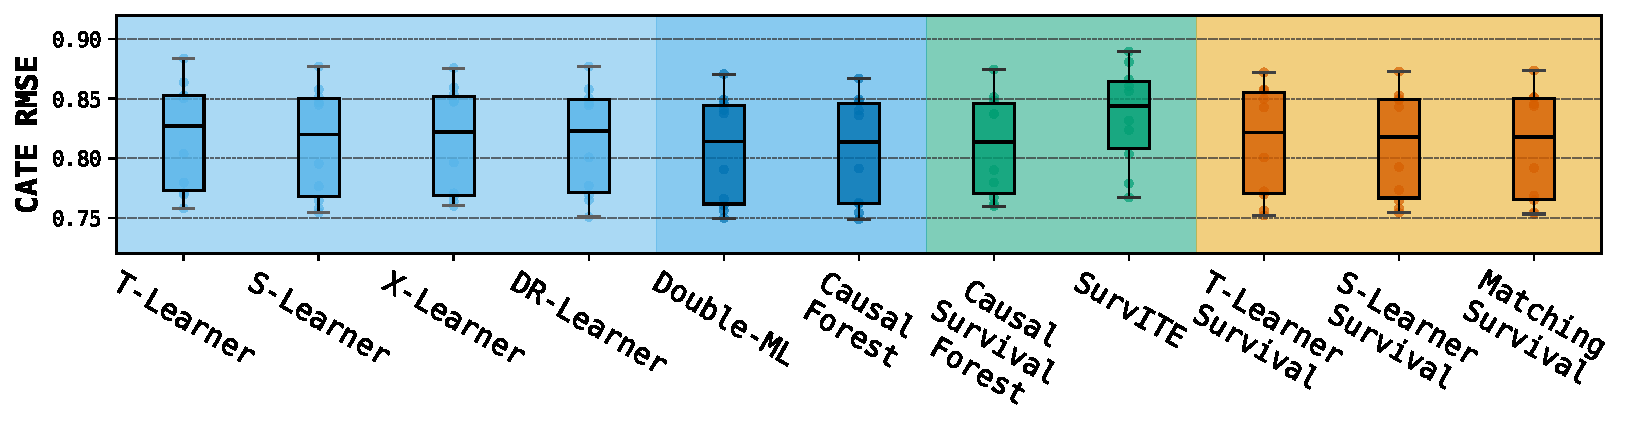
\includegraphics[width=\linewidth]{Appendices/appendix-ch04/images/figure_results_updated/cate_rmse/Scenario_B_OBS-CPS_cate_mse.pdf}
        
    \end{minipage}}
    \hfill
    \subfloat[{RCT: \ChFourBlackCross, Ignorability: \ChFourBlackCross, Positivity: \ChFourGrayCheck, Ignorable Censoring: \ChFourGrayCheck}]{\begin{minipage}[t]{0.49\textwidth}
        \centering
        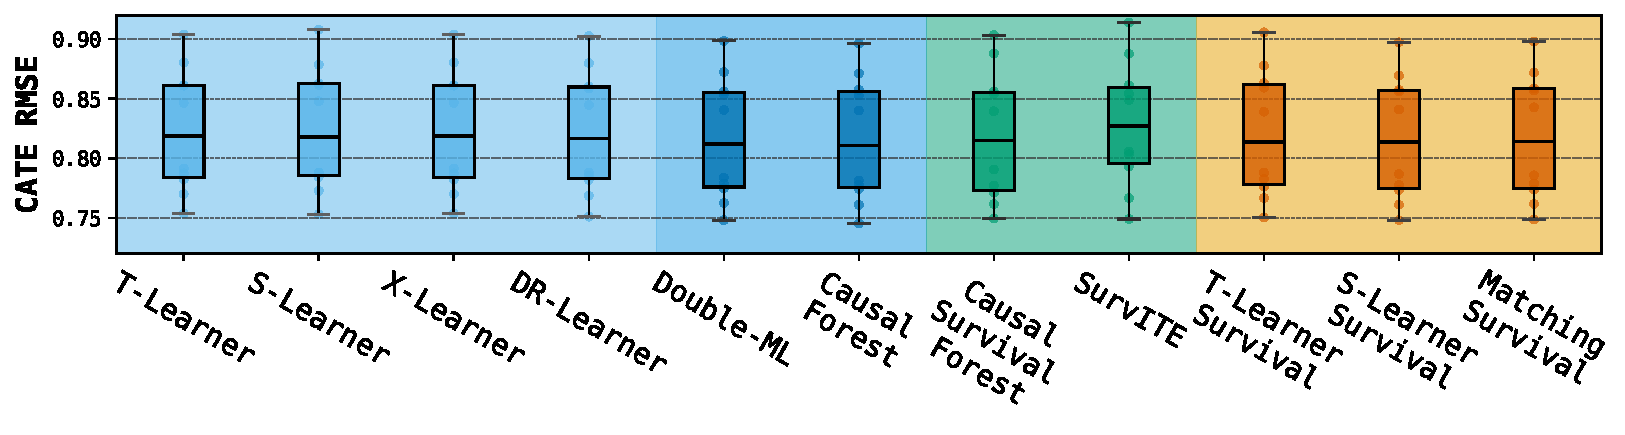
\includegraphics[width=\linewidth]{Appendices/appendix-ch04/images/figure_results_updated/cate_rmse/Scenario_B_OBS-UConf_cate_mse.pdf}
        
    \end{minipage}}

    

    \subfloat[{RCT: \ChFourBlackCross, Ignorability: \ChFourGrayCheck, Positivity: \ChFourBlackCross, Ignorable Censoring: \ChFourGrayCheck}]{\begin{minipage}[t]{0.49\textwidth}
        \centering
        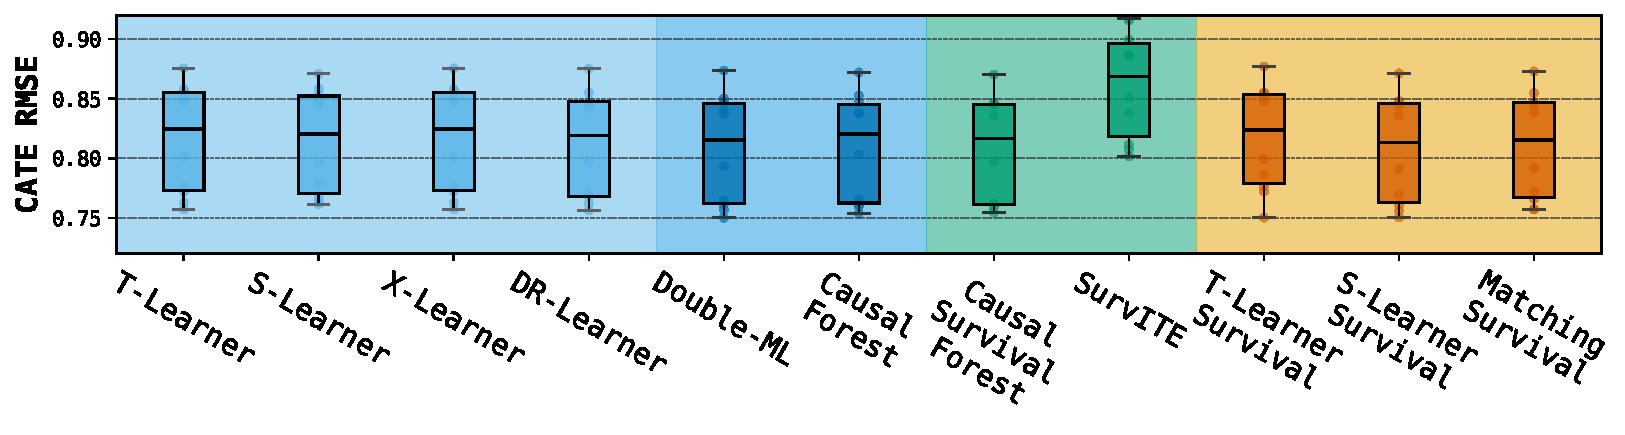
\includegraphics[width=\linewidth]{Appendices/appendix-ch04/images/figure_results_updated/cate_rmse/Scenario_B_OBS-NoPos_cate_mse.pdf}
        
    \end{minipage}}
    \hfill
    \subfloat[{RCT: \ChFourBlackCross, Ignorability: \ChFourGrayCheck, Positivity: \ChFourGrayCheck, Ignorable Censoring: \ChFourBlackCross}]{\begin{minipage}[t]{0.49\textwidth}
        \centering
        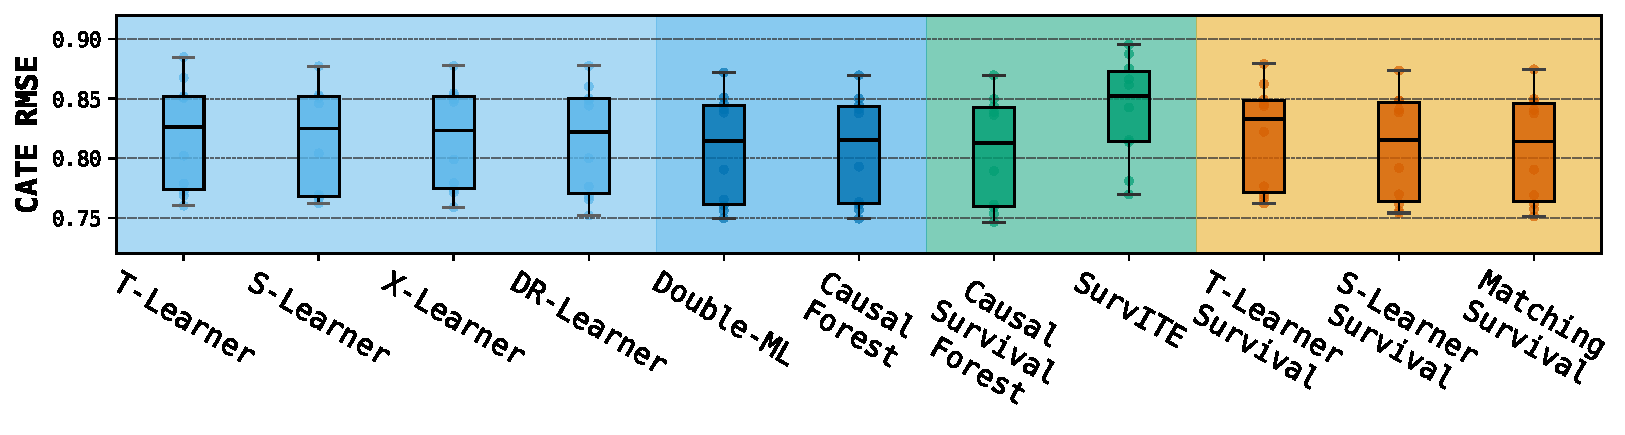
\includegraphics[width=\linewidth]{Appendices/appendix-ch04/images/figure_results_updated/cate_rmse/Scenario_B_OBS-CPS-IC_cate_mse.pdf}
        
    \end{minipage}}

    

    \subfloat[{RCT: \ChFourBlackCross, Ignorability: \ChFourBlackCross, Positivity: \ChFourGrayCheck, Ignorable Censoring: \ChFourBlackCross}]{\begin{minipage}[t]{0.49\textwidth}
        \centering
        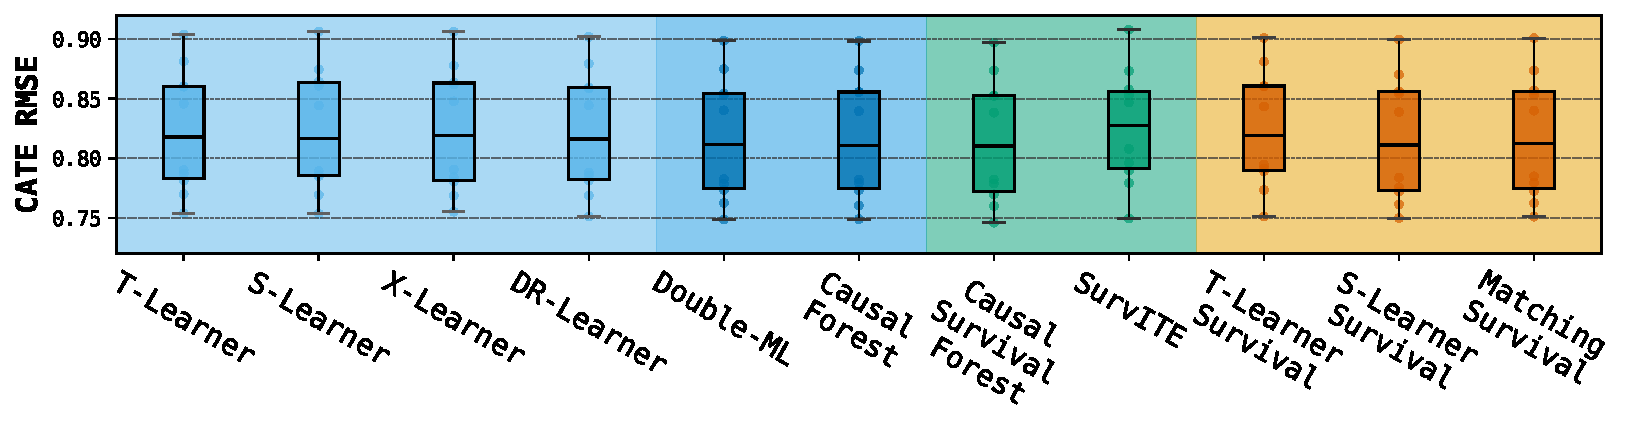
\includegraphics[width=\linewidth]{Appendices/appendix-ch04/images/figure_results_updated/cate_rmse/Scenario_B_OBS-UConf-IC_cate_mse.pdf}
        
    \end{minipage}}
    \hfill
    \subfloat[{RCT: \ChFourBlackCross, Ignorability: \ChFourGrayCheck, Positivity: \ChFourBlackCross, Ignorable Censoring: \ChFourBlackCross}]{\begin{minipage}[t]{0.49\textwidth}
        \centering
        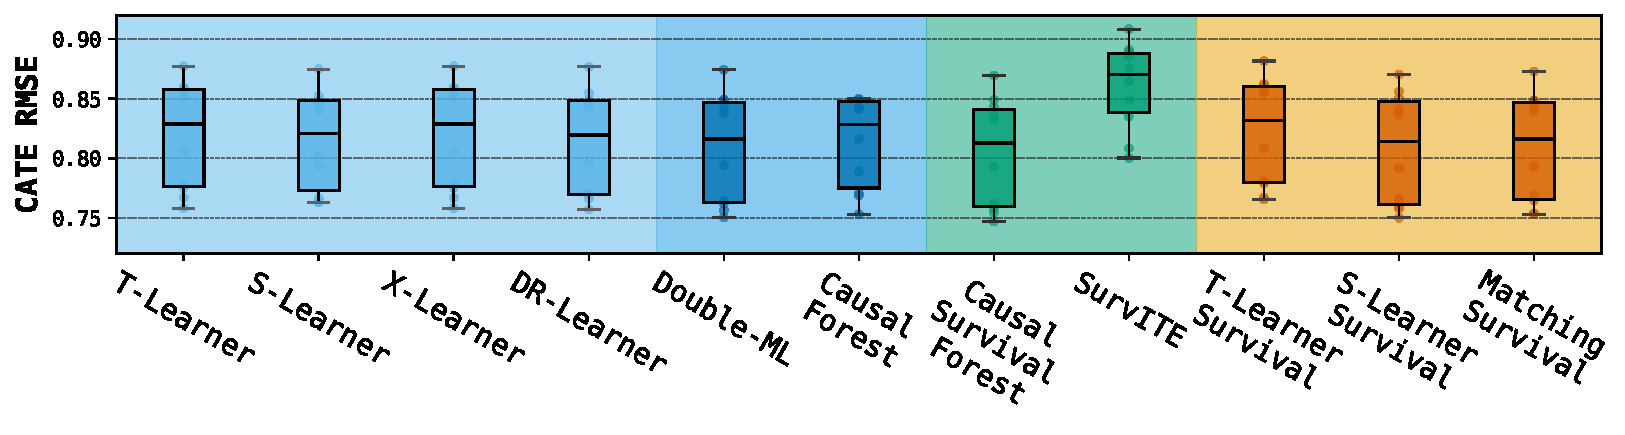
\includegraphics[width=\linewidth]{Appendices/appendix-ch04/images/figure_results_updated/cate_rmse/Scenario_B_OBS-NoPos-IC_cate_mse.pdf}
        
    \end{minipage}}

            \end{minipage}%
    }
    

    
    
}
\end{figure}



% 

% Secnario C

% !TeX root = ../../../main.tex
\begin{figure}[htbp]
\ChFourFloatContents{ch04:fig:cate_mse_grid_scenario_C}{\caption{CATE RMSE across different experiments in Scenario \texttt{C}.}}{
    \centering

    \resizebox{0.95\textwidth}{!}{%
        \begin{minipage}{1\textwidth}


    \subfloat[{RCT: \ChFourGrayCheck (50\%), Ignorability: \ChFourGrayCheck, Positivity: \ChFourGrayCheck, Ign-Censoring: \ChFourGrayCheck}]{\begin{minipage}[t]{0.49\textwidth}
        \centering
        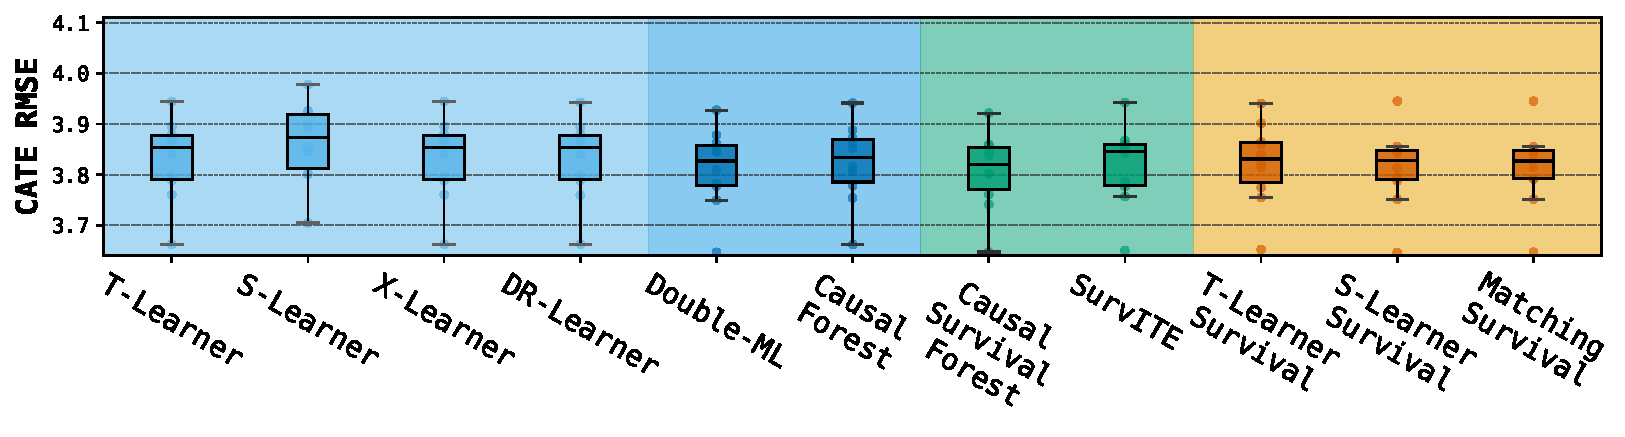
\includegraphics[width=\linewidth]{Appendices/appendix-ch04/images/figure_results_updated/cate_rmse/Scenario_C_RCT-50_cate_mse.pdf}
        
    \end{minipage}}
    \hfill
    \subfloat[{RCT: \ChFourGrayCheck (5\%), Ignorability: \ChFourGrayCheck, Positivity: \ChFourGrayCheck, Ign-Censoring: \ChFourGrayCheck}]{\begin{minipage}[t]{0.49\textwidth}
        \centering
        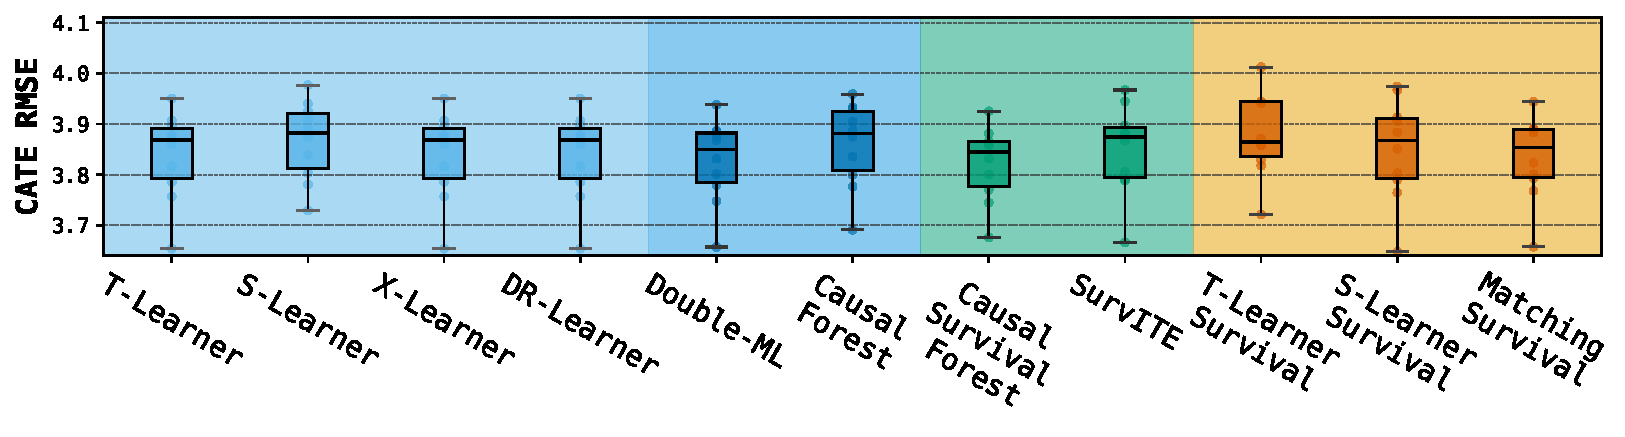
\includegraphics[width=\linewidth]{Appendices/appendix-ch04/images/figure_results_updated/cate_rmse/Scenario_C_RCT-5_cate_mse.pdf}
        
    \end{minipage}}

    

    \subfloat[{RCT: \ChFourBlackCross, Ignorability: \ChFourGrayCheck, Positivity: \ChFourGrayCheck, Ignorable Censoring: \ChFourGrayCheck}]{\begin{minipage}[t]{0.49\textwidth}
        \centering
        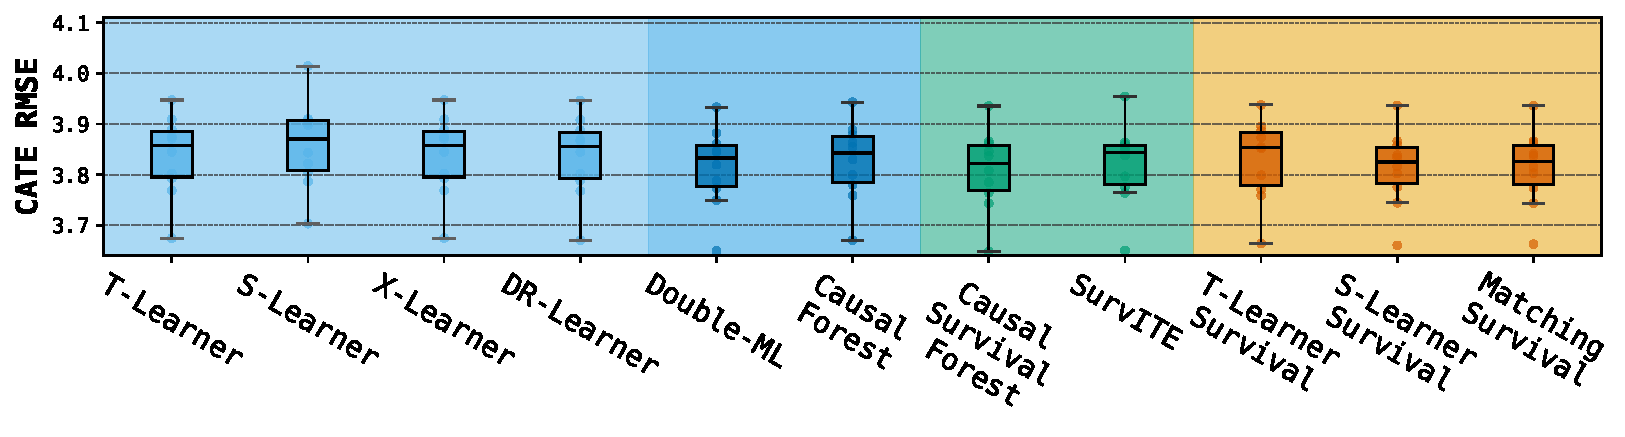
\includegraphics[width=\linewidth]{Appendices/appendix-ch04/images/figure_results_updated/cate_rmse/Scenario_C_OBS-CPS_cate_mse.pdf}
        
    \end{minipage}}
    \hfill
    \subfloat[{RCT: \ChFourBlackCross, Ignorability: \ChFourBlackCross, Positivity: \ChFourGrayCheck, Ignorable Censoring: \ChFourGrayCheck}]{\begin{minipage}[t]{0.49\textwidth}
        \centering
        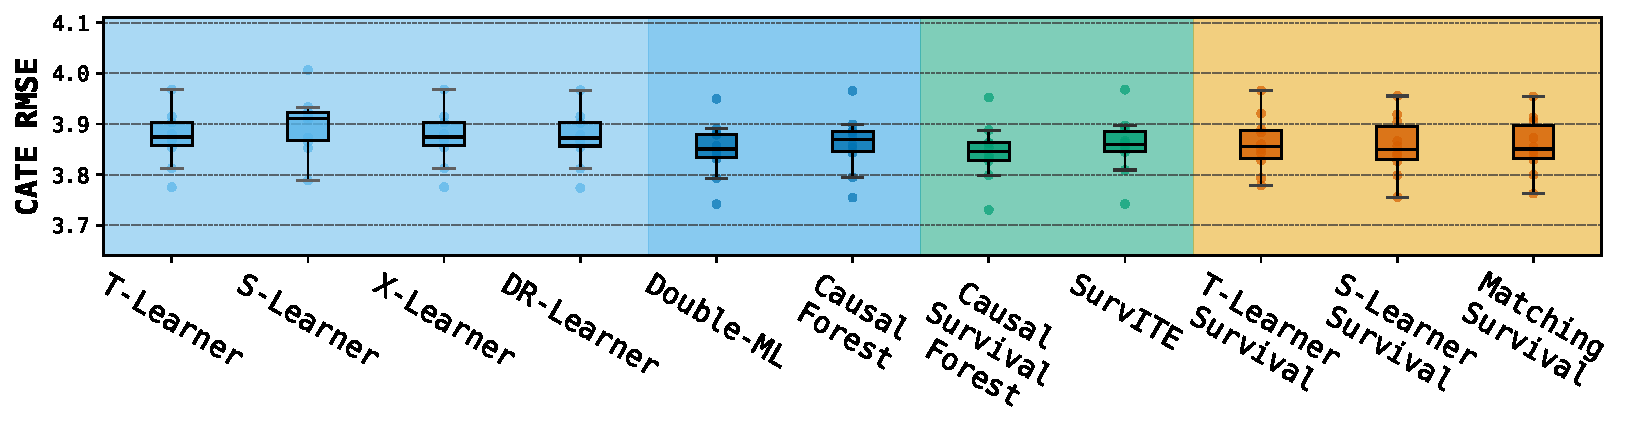
\includegraphics[width=\linewidth]{Appendices/appendix-ch04/images/figure_results_updated/cate_rmse/Scenario_C_OBS-UConf_cate_mse.pdf}
        
    \end{minipage}}

    

    \subfloat[{RCT: \ChFourBlackCross, Ignorability: \ChFourGrayCheck, Positivity: \ChFourBlackCross, Ignorable Censoring: \ChFourGrayCheck}]{\begin{minipage}[t]{0.49\textwidth}
        \centering
        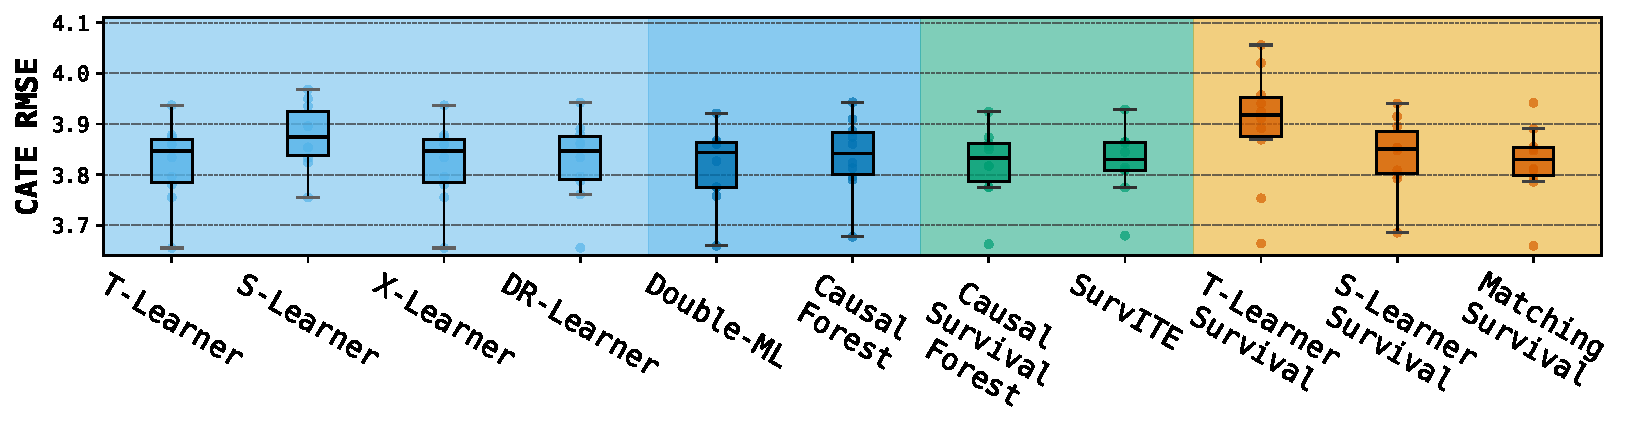
\includegraphics[width=\linewidth]{Appendices/appendix-ch04/images/figure_results_updated/cate_rmse/Scenario_C_OBS-NoPos_cate_mse.pdf}
        
    \end{minipage}}
    \hfill
    \subfloat[{RCT: \ChFourBlackCross, Ignorability: \ChFourGrayCheck, Positivity: \ChFourGrayCheck, Ignorable Censoring: \ChFourBlackCross}]{\begin{minipage}[t]{0.49\textwidth}
        \centering
        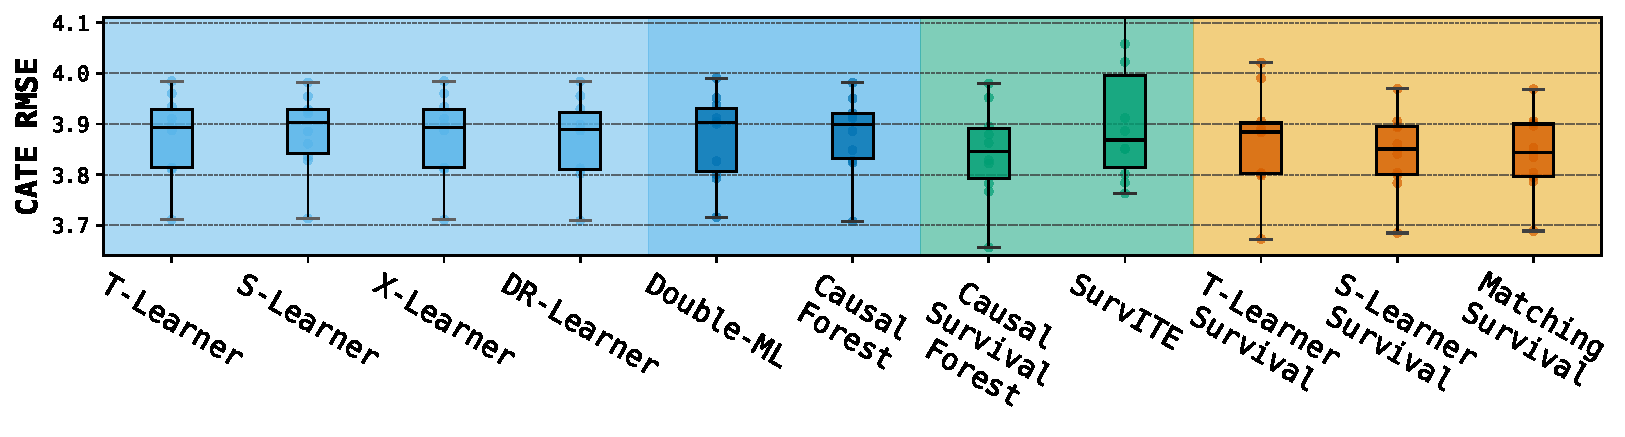
\includegraphics[width=\linewidth]{Appendices/appendix-ch04/images/figure_results_updated/cate_rmse/Scenario_C_OBS-CPS-IC_cate_mse.pdf}
        
    \end{minipage}}

    

    \subfloat[{RCT: \ChFourBlackCross, Ignorability: \ChFourBlackCross, Positivity: \ChFourGrayCheck, Ignorable Censoring: \ChFourBlackCross}]{\begin{minipage}[t]{0.49\textwidth}
        \centering
        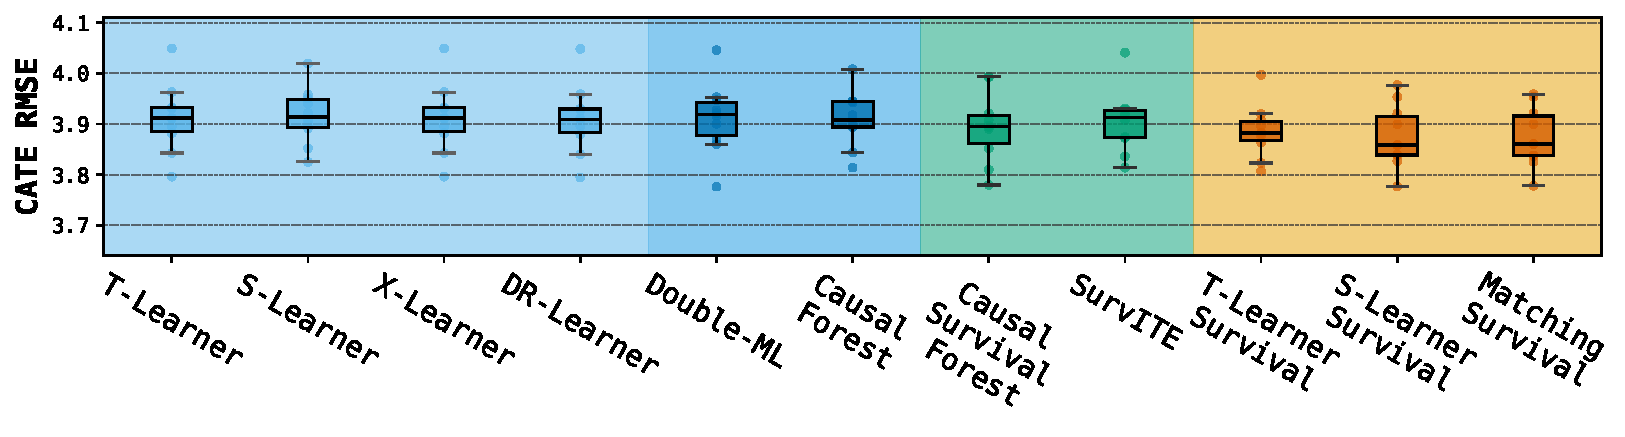
\includegraphics[width=\linewidth]{Appendices/appendix-ch04/images/figure_results_updated/cate_rmse/Scenario_C_OBS-UConf-IC_cate_mse.pdf}
        
    \end{minipage}}
    \hfill
    \subfloat[{RCT: \ChFourBlackCross, Ignorability: \ChFourGrayCheck, Positivity: \ChFourBlackCross, Ignorable Censoring: \ChFourBlackCross}]{\begin{minipage}[t]{0.49\textwidth}
        \centering
        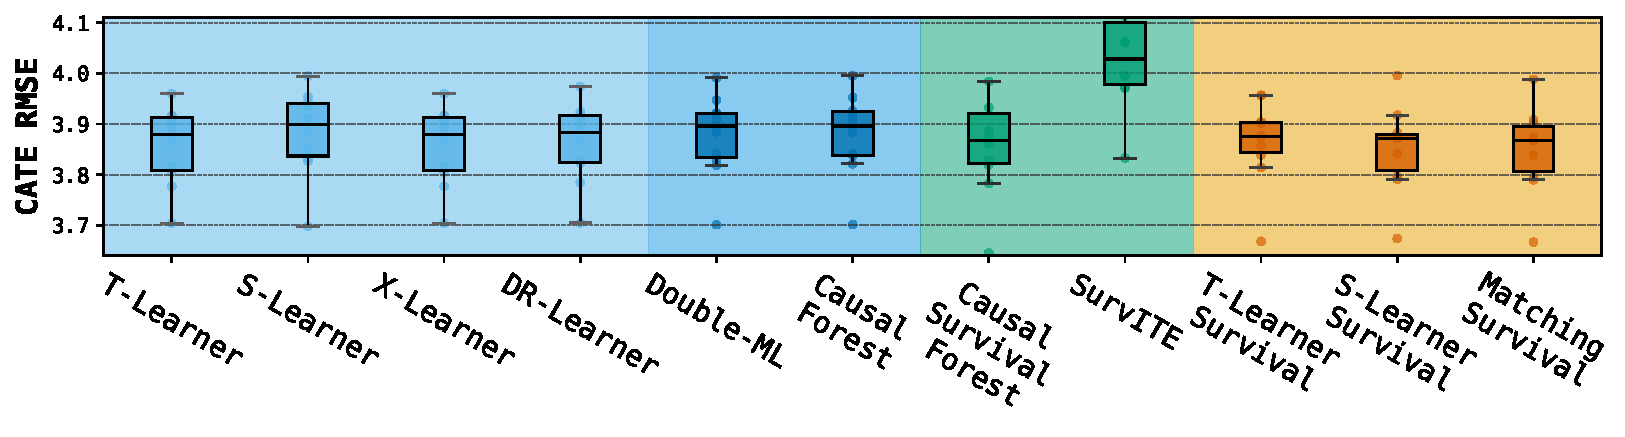
\includegraphics[width=\linewidth]{Appendices/appendix-ch04/images/figure_results_updated/cate_rmse/Scenario_C_OBS-NoPos-IC_cate_mse.pdf}
        
    \end{minipage}}

            \end{minipage}%
    }
    

    
    
}
\end{figure}




% 

% Scenario D

% !TeX root = ../../../main.tex
\begin{figure}[htbp]
\ChFourFloatContents{ch04:fig:cate_mse_grid_scenario_D}{\caption{CATE RMSE across different experiments in Scenario \texttt{D}.}}{
    \centering

    \resizebox{0.95\textwidth}{!}{%
        \begin{minipage}{1\textwidth}


    \subfloat[{RCT: \ChFourGrayCheck (50\%), Ignorability: \ChFourGrayCheck, Positivity: \ChFourGrayCheck, Ign-Censoring: \ChFourGrayCheck}]{\begin{minipage}[t]{0.49\textwidth}
        \centering
        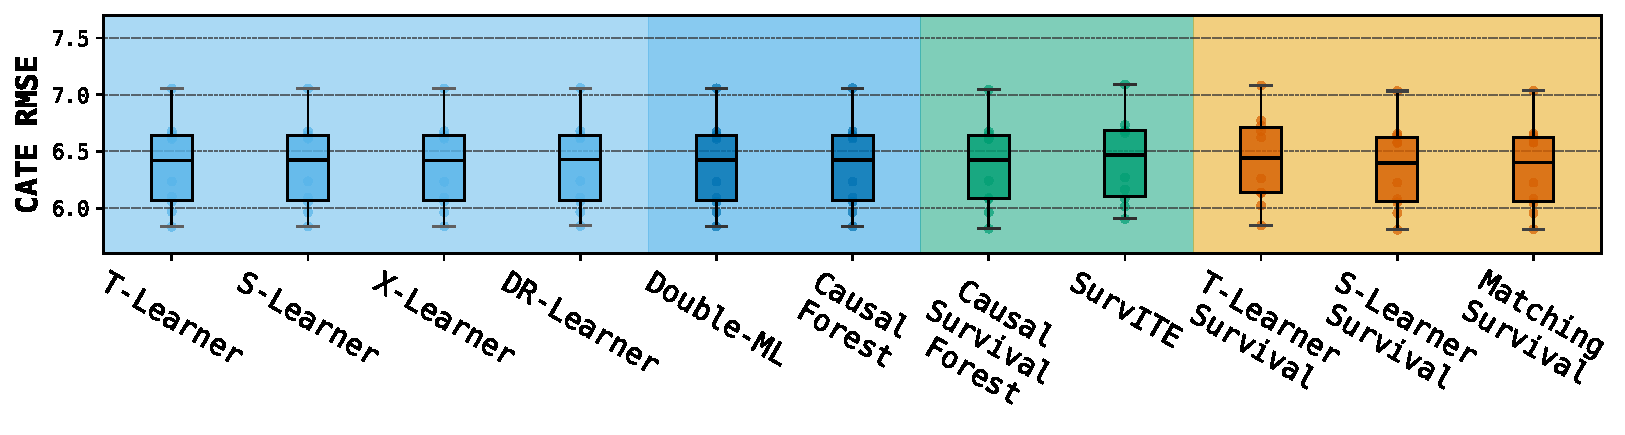
\includegraphics[width=\linewidth]{Appendices/appendix-ch04/images/figure_results_updated/cate_rmse/Scenario_D_RCT-50_cate_mse.pdf}
        
    \end{minipage}}
    \hfill
    \subfloat[{RCT: \ChFourGrayCheck (5\%), Ignorability: \ChFourGrayCheck, Positivity: \ChFourGrayCheck, Ign-Censoring: \ChFourGrayCheck}]{\begin{minipage}[t]{0.49\textwidth}
        \centering
        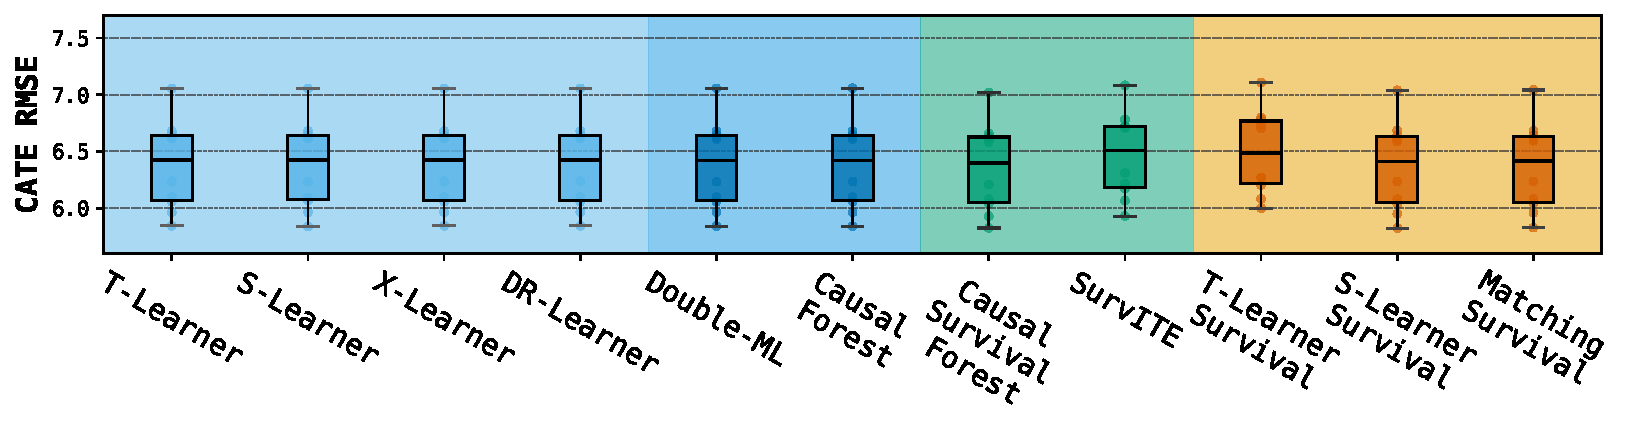
\includegraphics[width=\linewidth]{Appendices/appendix-ch04/images/figure_results_updated/cate_rmse/Scenario_D_RCT-5_cate_mse.pdf}
        
    \end{minipage}}

    

    \subfloat[{RCT: \ChFourBlackCross, Ignorability: \ChFourGrayCheck, Positivity: \ChFourGrayCheck, Ignorable Censoring: \ChFourGrayCheck}]{\begin{minipage}[t]{0.49\textwidth}
        \centering
        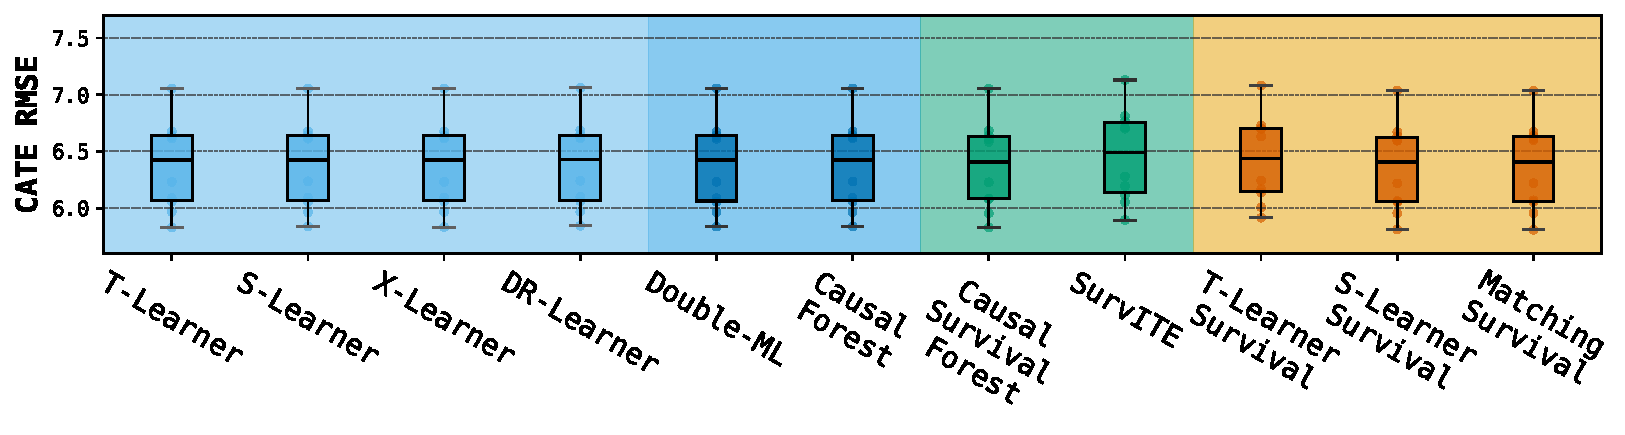
\includegraphics[width=\linewidth]{Appendices/appendix-ch04/images/figure_results_updated/cate_rmse/Scenario_D_OBS-CPS_cate_mse.pdf}
        
    \end{minipage}}
    \hfill
    \subfloat[{RCT: \ChFourBlackCross, Ignorability: \ChFourBlackCross, Positivity: \ChFourGrayCheck, Ignorable Censoring: \ChFourGrayCheck}]{\begin{minipage}[t]{0.49\textwidth}
        \centering
        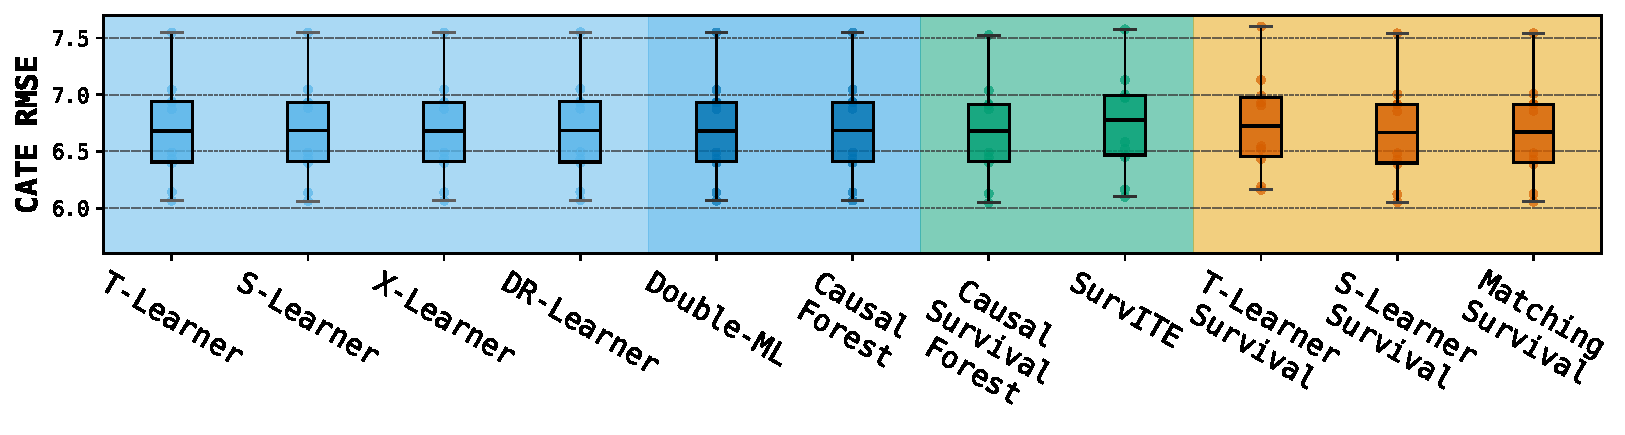
\includegraphics[width=\linewidth]{Appendices/appendix-ch04/images/figure_results_updated/cate_rmse/Scenario_D_OBS-UConf_cate_mse.pdf}
        
    \end{minipage}}

    

    \subfloat[{RCT: \ChFourBlackCross, Ignorability: \ChFourGrayCheck, Positivity: \ChFourBlackCross, Ignorable Censoring: \ChFourGrayCheck}]{\begin{minipage}[t]{0.49\textwidth}
        \centering
        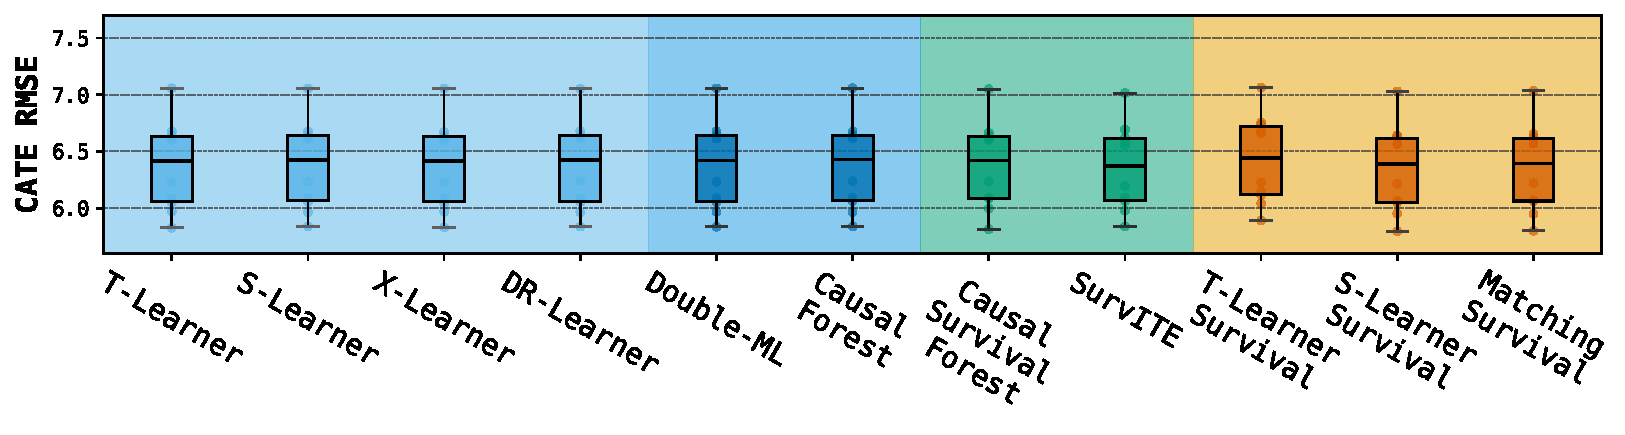
\includegraphics[width=\linewidth]{Appendices/appendix-ch04/images/figure_results_updated/cate_rmse/Scenario_D_OBS-NoPos_cate_mse.pdf}
        
    \end{minipage}}
    \hfill
    \subfloat[{RCT: \ChFourBlackCross, Ignorability: \ChFourGrayCheck, Positivity: \ChFourGrayCheck, Ignorable Censoring: \ChFourBlackCross}]{\begin{minipage}[t]{0.49\textwidth}
        \centering
        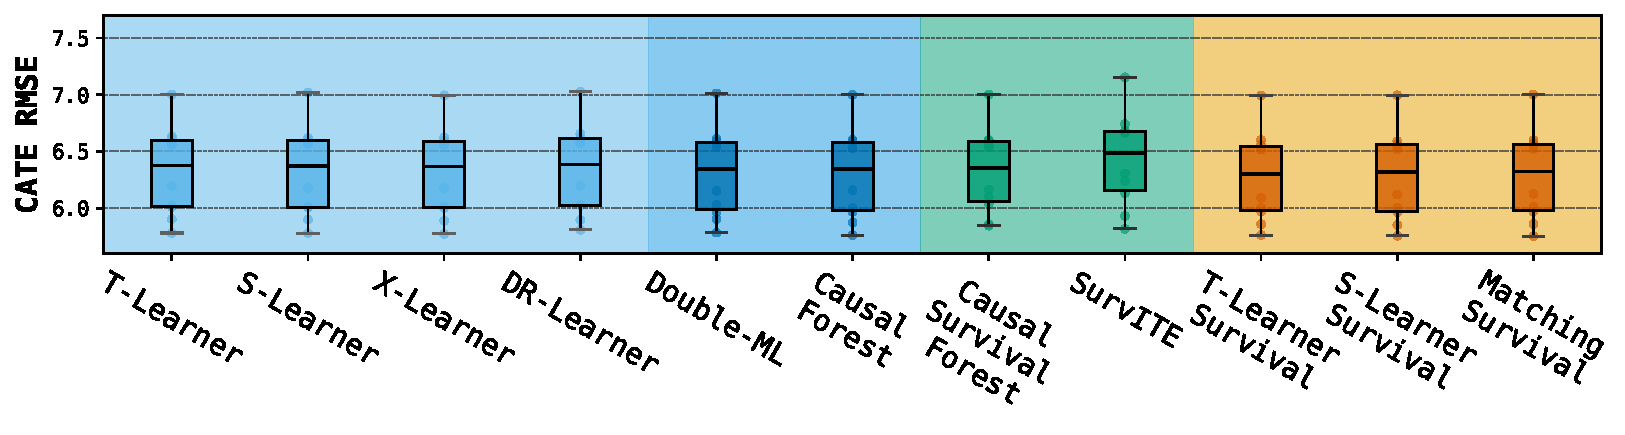
\includegraphics[width=\linewidth]{Appendices/appendix-ch04/images/figure_results_updated/cate_rmse/Scenario_D_OBS-CPS-IC_cate_mse.pdf}
        
    \end{minipage}}

    

    \subfloat[{RCT: \ChFourBlackCross, Ignorability: \ChFourBlackCross, Positivity: \ChFourGrayCheck, Ignorable Censoring: \ChFourBlackCross}]{\begin{minipage}[t]{0.49\textwidth}
        \centering
        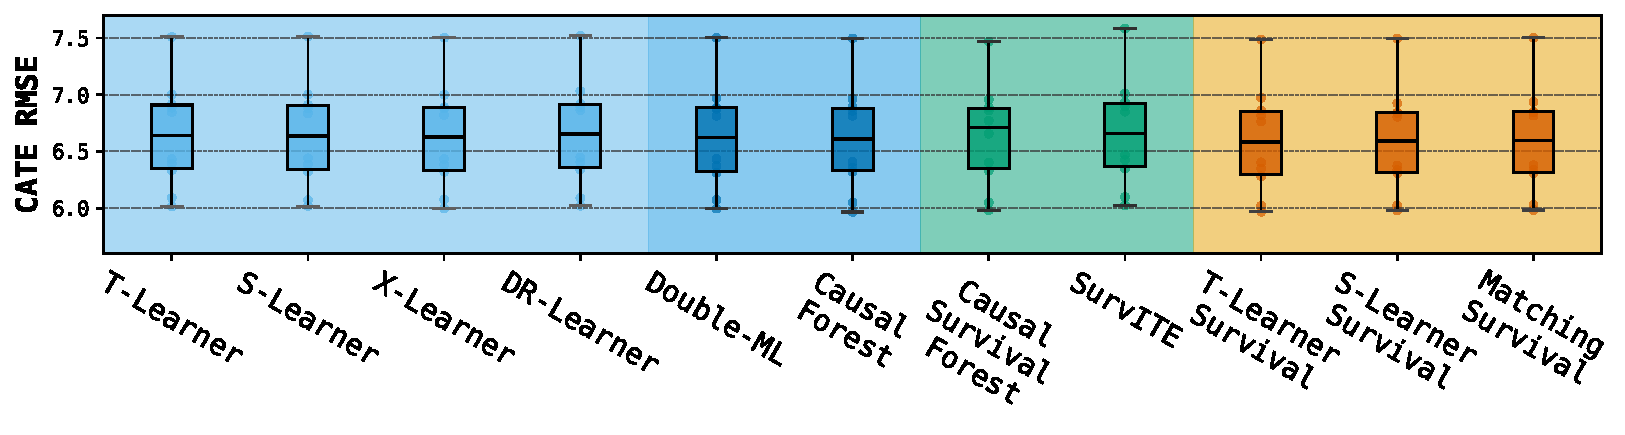
\includegraphics[width=\linewidth]{Appendices/appendix-ch04/images/figure_results_updated/cate_rmse/Scenario_D_OBS-UConf-IC_cate_mse.pdf}
        
    \end{minipage}}
    \hfill
    \subfloat[{RCT: \ChFourBlackCross, Ignorability: \ChFourGrayCheck, Positivity: \ChFourBlackCross, Ignorable Censoring: \ChFourBlackCross}]{\begin{minipage}[t]{0.49\textwidth}
        \centering
        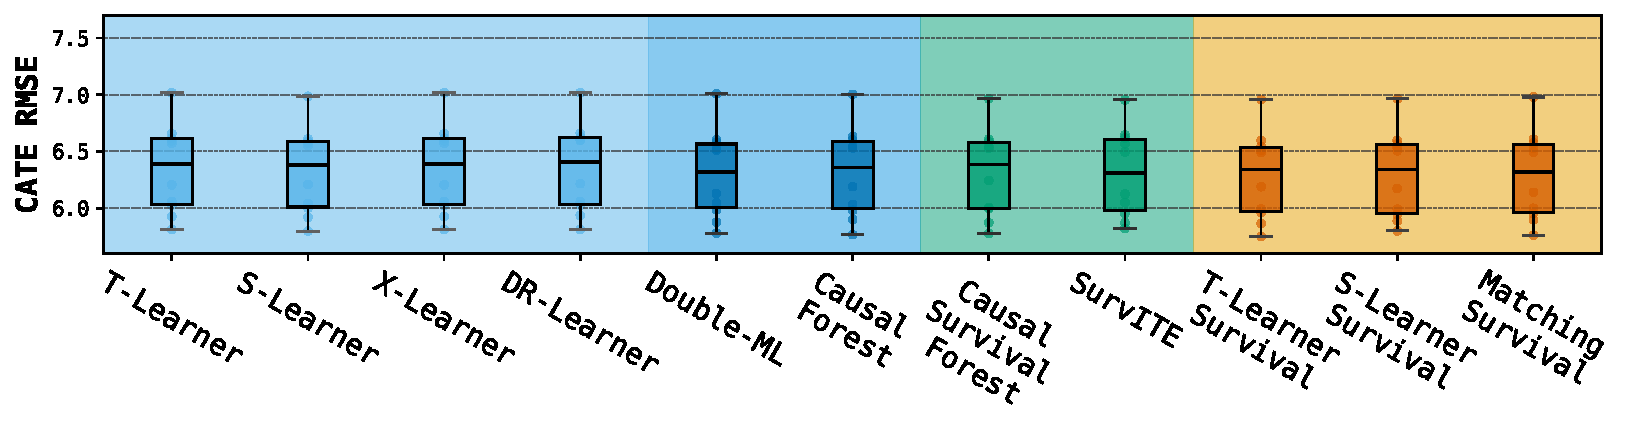
\includegraphics[width=\linewidth]{Appendices/appendix-ch04/images/figure_results_updated/cate_rmse/Scenario_D_OBS-NoPos-IC_cate_mse.pdf}
        
    \end{minipage}}

            \end{minipage}%
    }
    

    
    
}
\end{figure}


% 

% Secnario E

% !TeX root = ../../../main.tex
\begin{figure}[htbp]
\ChFourFloatContents{ch04:fig:cate_mse_grid_scenario_E}{\caption{CATE RMSE across different experiments in Scenario \texttt{E}.}}{
    \centering

    \resizebox{0.95\textwidth}{!}{%
        \begin{minipage}{1\textwidth}


    \subfloat[{RCT: \ChFourGrayCheck (50\%), Ignorability: \ChFourGrayCheck, Positivity: \ChFourGrayCheck, Ign-Censoring: \ChFourGrayCheck}]{\begin{minipage}[t]{0.49\textwidth}
        \centering
        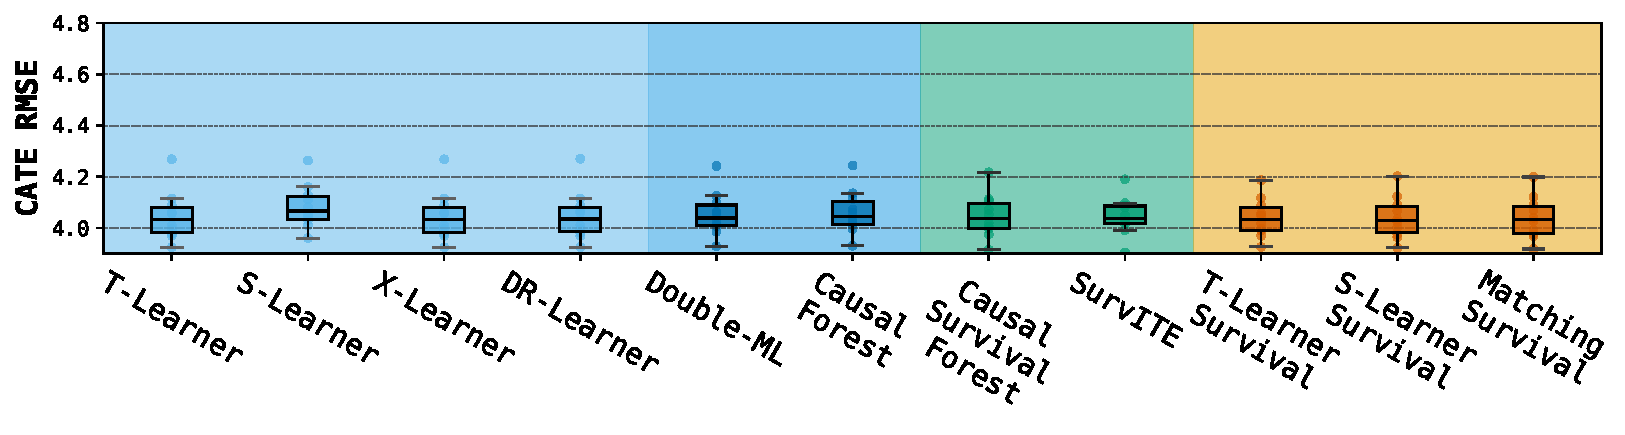
\includegraphics[width=\linewidth]{Appendices/appendix-ch04/images/figure_results_updated/cate_rmse/Scenario_E_RCT-50_cate_mse.pdf}
        
    \end{minipage}}
    \hfill
    \subfloat[{RCT: \ChFourGrayCheck (5\%), Ignorability: \ChFourGrayCheck, Positivity: \ChFourGrayCheck, Ign-Censoring: \ChFourGrayCheck}]{\begin{minipage}[t]{0.49\textwidth}
        \centering
        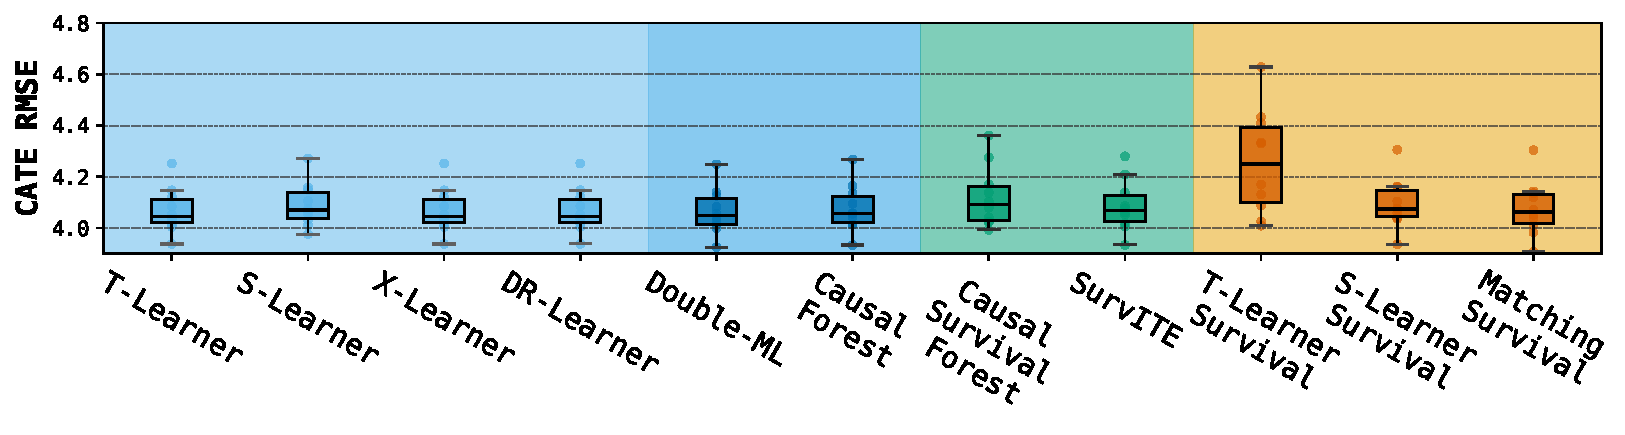
\includegraphics[width=\linewidth]{Appendices/appendix-ch04/images/figure_results_updated/cate_rmse/Scenario_E_RCT-5_cate_mse.pdf}
        
    \end{minipage}}

    

    \subfloat[{RCT: \ChFourBlackCross, Ignorability: \ChFourGrayCheck, Positivity: \ChFourGrayCheck, Ignorable Censoring: \ChFourGrayCheck}]{\begin{minipage}[t]{0.49\textwidth}
        \centering
        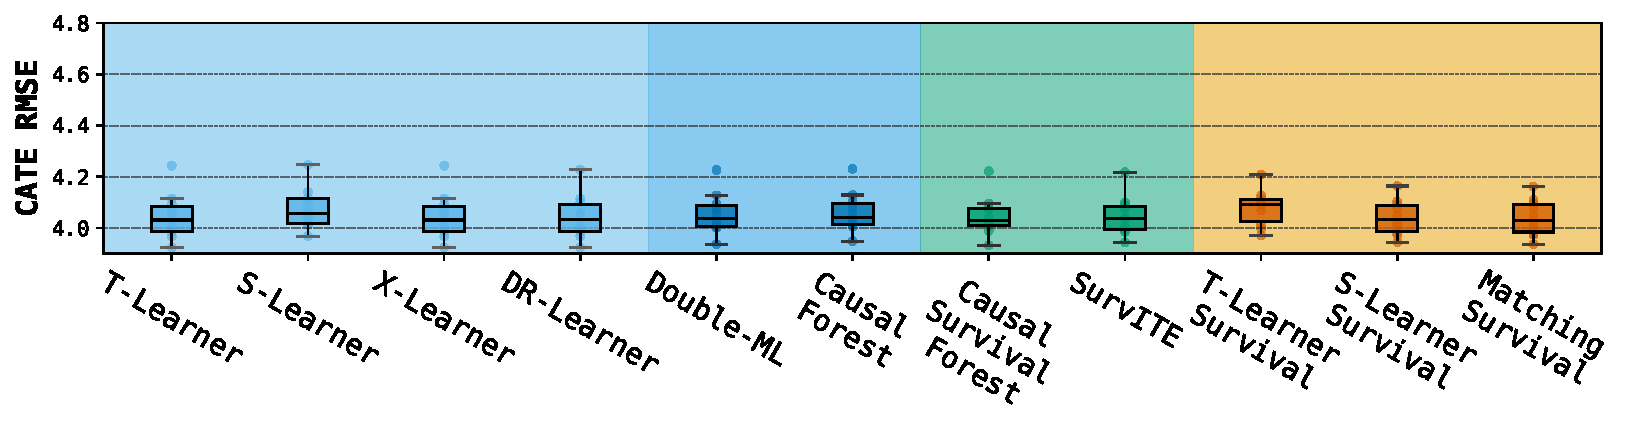
\includegraphics[width=\linewidth]{Appendices/appendix-ch04/images/figure_results_updated/cate_rmse/Scenario_E_OBS-CPS_cate_mse.pdf}
        
    \end{minipage}}
    \hfill
    \subfloat[{RCT: \ChFourBlackCross, Ignorability: \ChFourBlackCross, Positivity: \ChFourGrayCheck, Ignorable Censoring: \ChFourGrayCheck}]{\begin{minipage}[t]{0.49\textwidth}
        \centering
        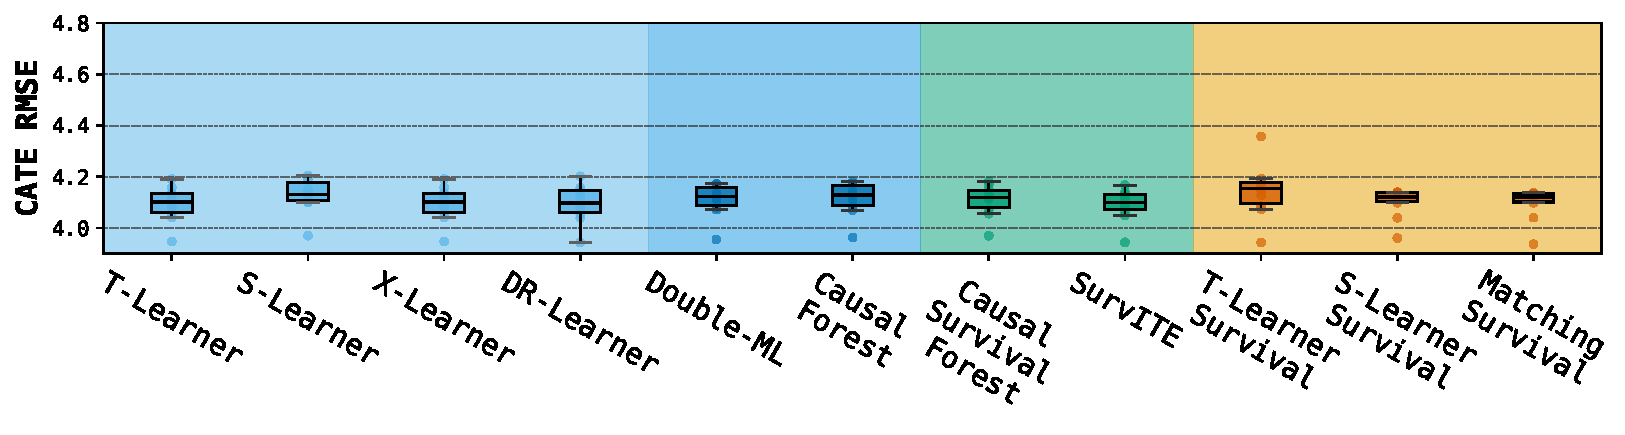
\includegraphics[width=\linewidth]{Appendices/appendix-ch04/images/figure_results_updated/cate_rmse/Scenario_E_OBS-UConf_cate_mse.pdf}
        
    \end{minipage}}

    

    \subfloat[{RCT: \ChFourBlackCross, Ignorability: \ChFourGrayCheck, Positivity: \ChFourBlackCross, Ignorable Censoring: \ChFourGrayCheck}]{\begin{minipage}[t]{0.49\textwidth}
        \centering
        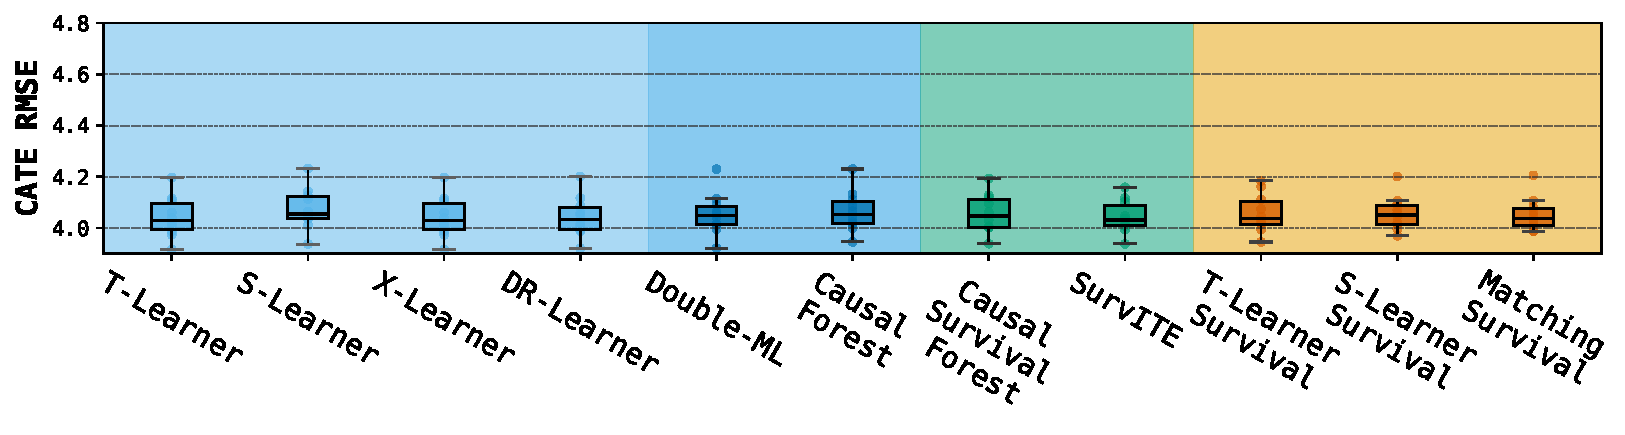
\includegraphics[width=\linewidth]{Appendices/appendix-ch04/images/figure_results_updated/cate_rmse/Scenario_E_OBS-NoPos_cate_mse.pdf}
        
    \end{minipage}}
    \hfill
    \subfloat[{RCT: \ChFourBlackCross, Ignorability: \ChFourGrayCheck, Positivity: \ChFourGrayCheck, Ignorable Censoring: \ChFourBlackCross}]{\begin{minipage}[t]{0.49\textwidth}
        \centering
        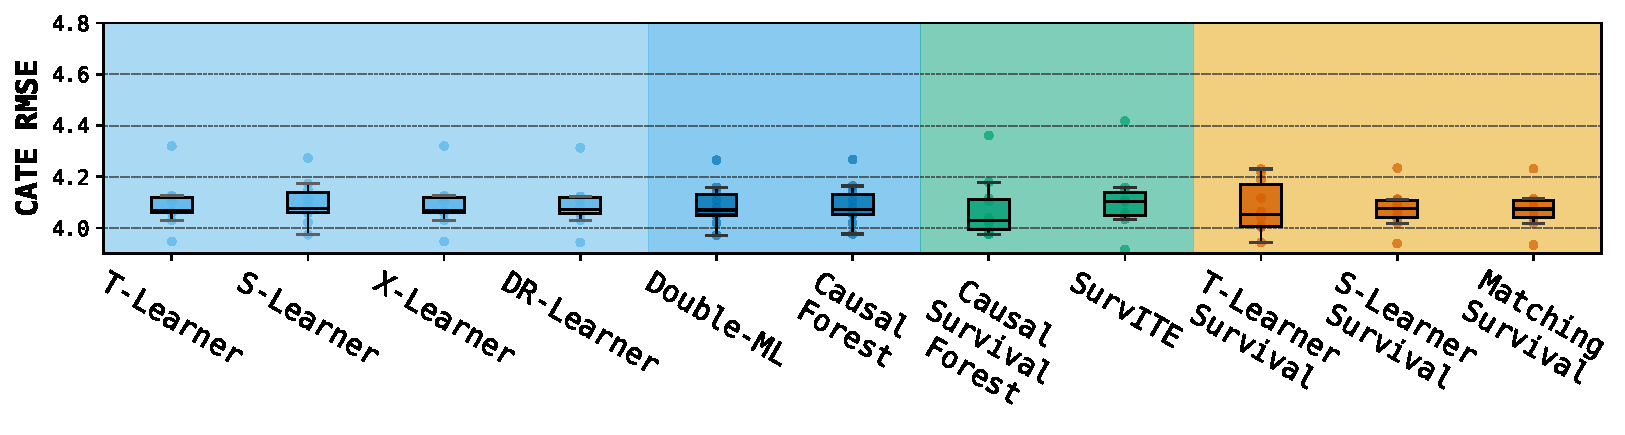
\includegraphics[width=\linewidth]{Appendices/appendix-ch04/images/figure_results_updated/cate_rmse/Scenario_E_OBS-CPS-IC_cate_mse.pdf}
        
    \end{minipage}}

    

    \subfloat[{RCT: \ChFourBlackCross, Ignorability: \ChFourBlackCross, Positivity: \ChFourGrayCheck, Ignorable Censoring: \ChFourBlackCross}]{\begin{minipage}[t]{0.49\textwidth}
        \centering
        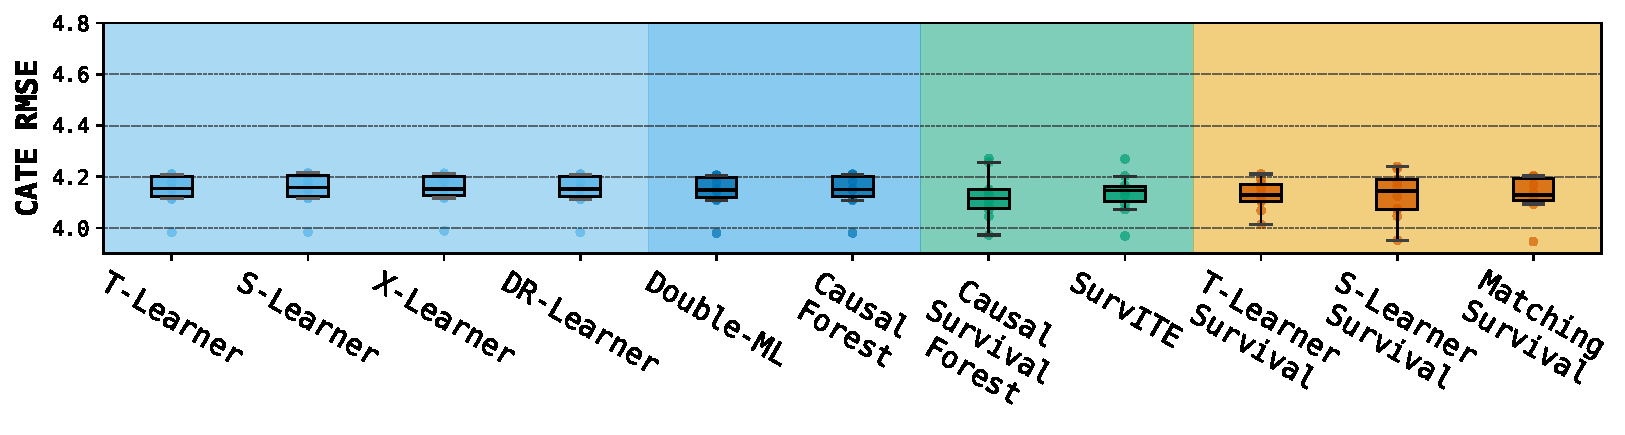
\includegraphics[width=\linewidth]{Appendices/appendix-ch04/images/figure_results_updated/cate_rmse/Scenario_E_OBS-UConf-IC_cate_mse.pdf}
        
    \end{minipage}}
    \hfill
    \subfloat[{RCT: \ChFourBlackCross, Ignorability: \ChFourGrayCheck, Positivity: \ChFourBlackCross, Ignorable Censoring: \ChFourBlackCross}]{\begin{minipage}[t]{0.49\textwidth}
        \centering
        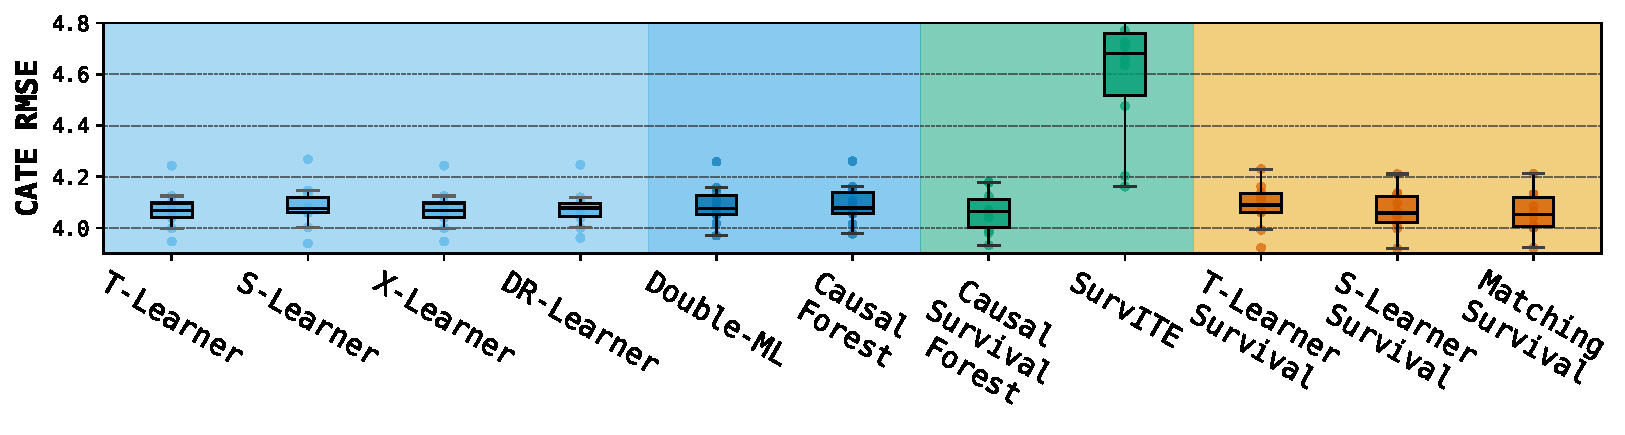
\includegraphics[width=\linewidth]{Appendices/appendix-ch04/images/figure_results_updated/cate_rmse/Scenario_E_OBS-NoPos-IC_cate_mse.pdf}
        
    \end{minipage}}

            \end{minipage}%
    }
    

    
    
}
\end{figure}






%%%%%%%%%%%%%%%%%%%%%%%%%%%%%%%%%%%%%%%%%%%%%%%%%%%%%%%%%%%%
%%%%%%%%%%%%%%%%%%%%%%%%%%%%%%%%%%%%%%%%%%%%%%%%%%%%%%%%%%%%
%%%%%%%%%%%%%%%%%%%%%%%%%%%%%%%%%%%%%%%%%%%%%%%%%%%%%%%%%%%%

\subsubsection{Figure results - ATE bias} \label{ch04:app:more-ate-plots}

This section presents the ATE bias results for each family of causal inference methods across various survival scenarios.
As with the CATE RMSE results in Appendix~\ref{ch04:app:more-cate-mse-plots}, we display performance under 8 distinct causal configurations per scenario, each varying in treatment assignment (RCT vs. observational), ignorability, positivity, and censoring assumptions.

For each survival scenario and causal configuration, the model shown corresponds to the best hyperparameter setting and base model configuration selected based on CATE RMSE performance on the validation set --- ATE bias was not used for model selection for consistent results with other sections.
The reported ATE bias values are computed on the test set and defined as the difference between the \emph{predicted ATE} from the test population and the \emph{true ATE} in the full population.

Each box plot represents results from 10 independent experimental repeats to account for random seed variability.
For meta-learners and double machine learning models, which by design can provide 95\% confidence intervals for ATE estimates, we also include these intervals in the plots---adjusted accordingly to center around the ATE bias.
These confidence intervals are obtained via 100 bootstrap samples and are notably wider than the variability observed across the 10 experimental repeats.
The zero bias line is shown as a dashed reference line.

% Secnario A

% !TeX root = ../../../main.tex
\begin{figure}[htbp]
\ChFourFloatContents{ch04:fig:ate_bias_grid_scenario_A}{\caption{ATE Bias across different experiments in Scenario \texttt{A}.}}{
    \centering

            \resizebox{0.95\textwidth}{!}{%
        \begin{minipage}{1\textwidth}

    \subfloat[{RCT: \ChFourGrayCheck (50\%), Ignorability: \ChFourGrayCheck, Positivity: \ChFourGrayCheck, Ign-Censoring: \ChFourGrayCheck}]{\begin{minipage}[t]{0.49\textwidth}
        \centering
        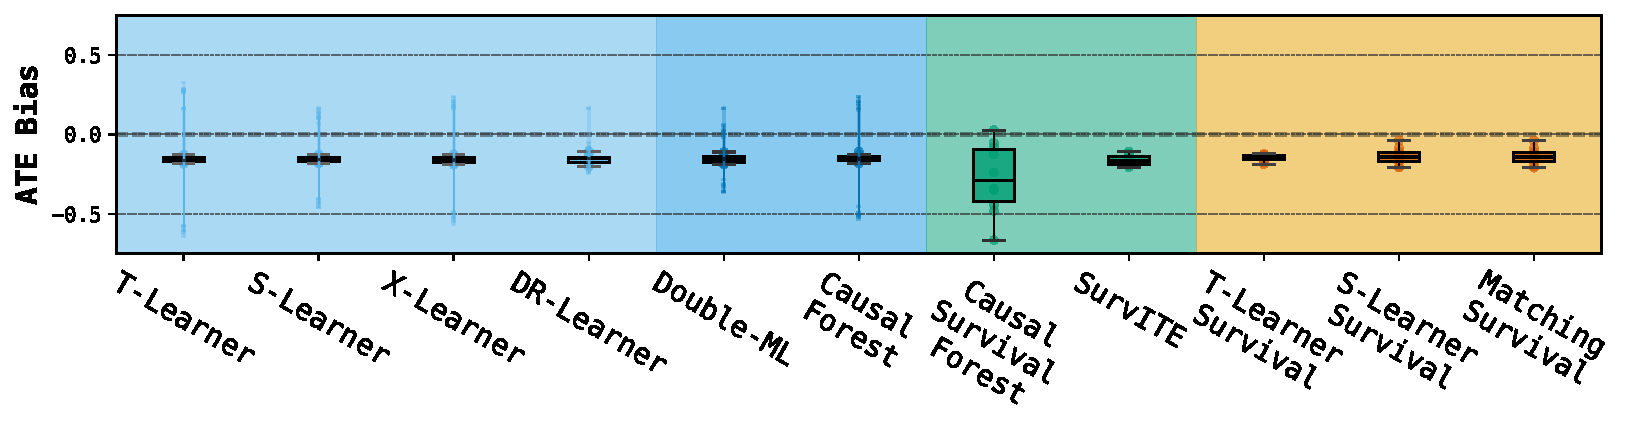
\includegraphics[width=\linewidth]{Appendices/appendix-ch04/images/figure_results_updated/ate_bias/Scenario_A_RCT-50_ate_bias.pdf}
        
    \end{minipage}}
    \hfill
    \subfloat[{RCT: \ChFourGrayCheck (5\%), Ignorability: \ChFourGrayCheck, Positivity: \ChFourGrayCheck, Ign-Censoring: \ChFourGrayCheck}]{\begin{minipage}[t]{0.49\textwidth}
        \centering
        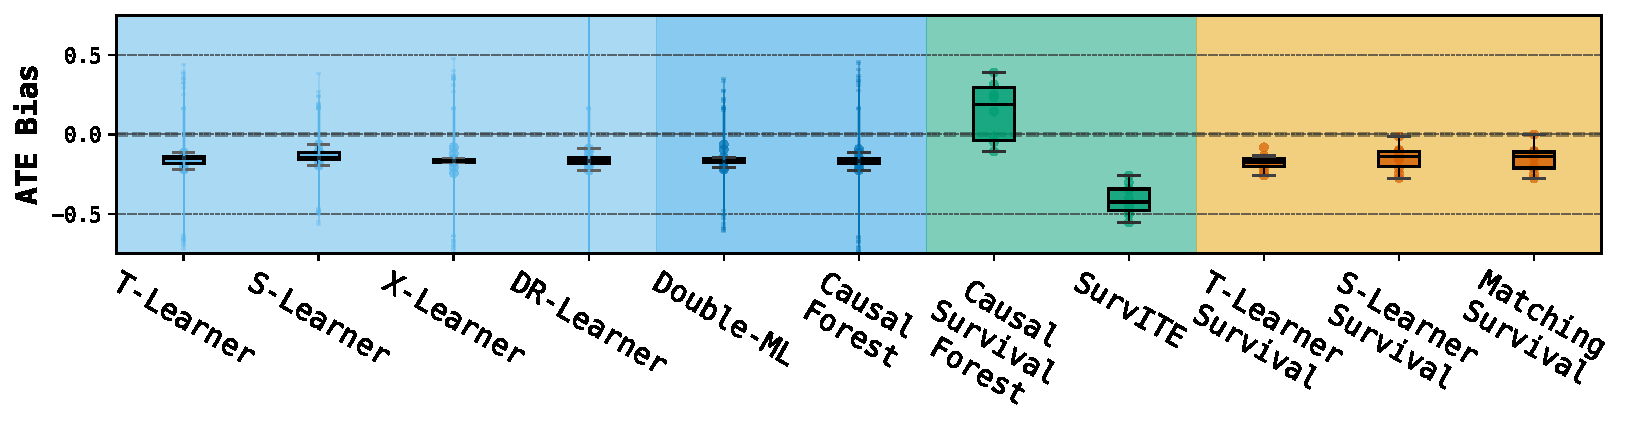
\includegraphics[width=\linewidth]{Appendices/appendix-ch04/images/figure_results_updated/ate_bias/Scenario_A_RCT-5_ate_bias.pdf}
        
    \end{minipage}}

    

    \subfloat[{RCT: \ChFourBlackCross, Ignorability: \ChFourGrayCheck, Positivity: \ChFourGrayCheck, Ignorable Censoring: \ChFourGrayCheck}]{\begin{minipage}[t]{0.49\textwidth}
        \centering
        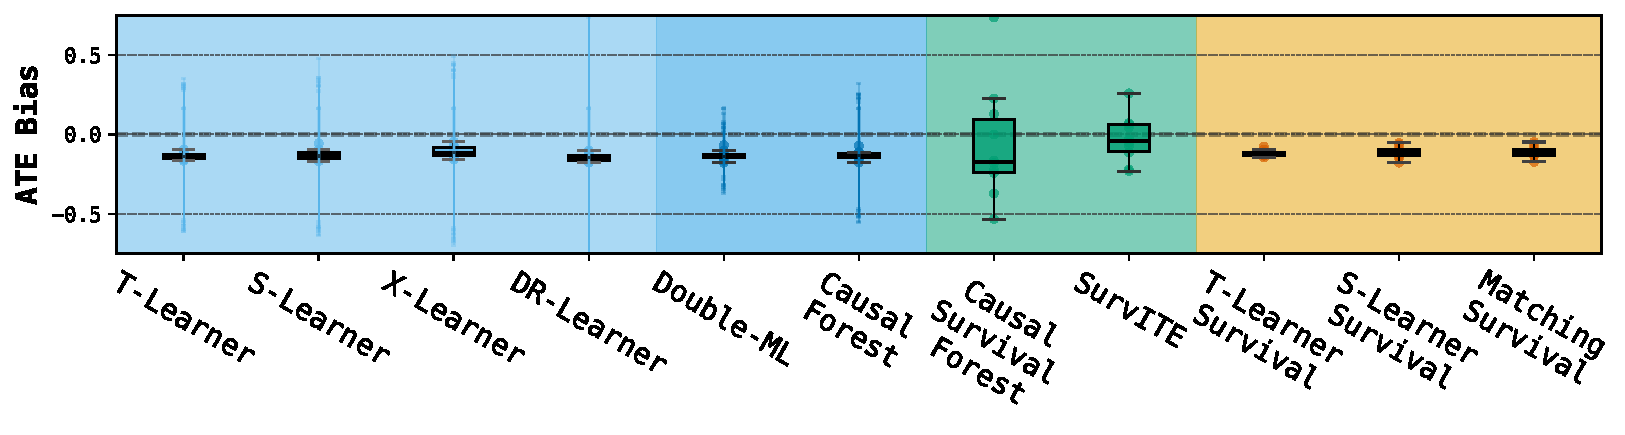
\includegraphics[width=\linewidth]{Appendices/appendix-ch04/images/figure_results_updated/ate_bias/Scenario_A_OBS-CPS_ate_bias.pdf}
        
    \end{minipage}}
    \hfill
    \subfloat[{RCT: \ChFourBlackCross, Ignorability: \ChFourBlackCross, Positivity: \ChFourGrayCheck, Ignorable Censoring: \ChFourGrayCheck}]{\begin{minipage}[t]{0.49\textwidth}
        \centering
        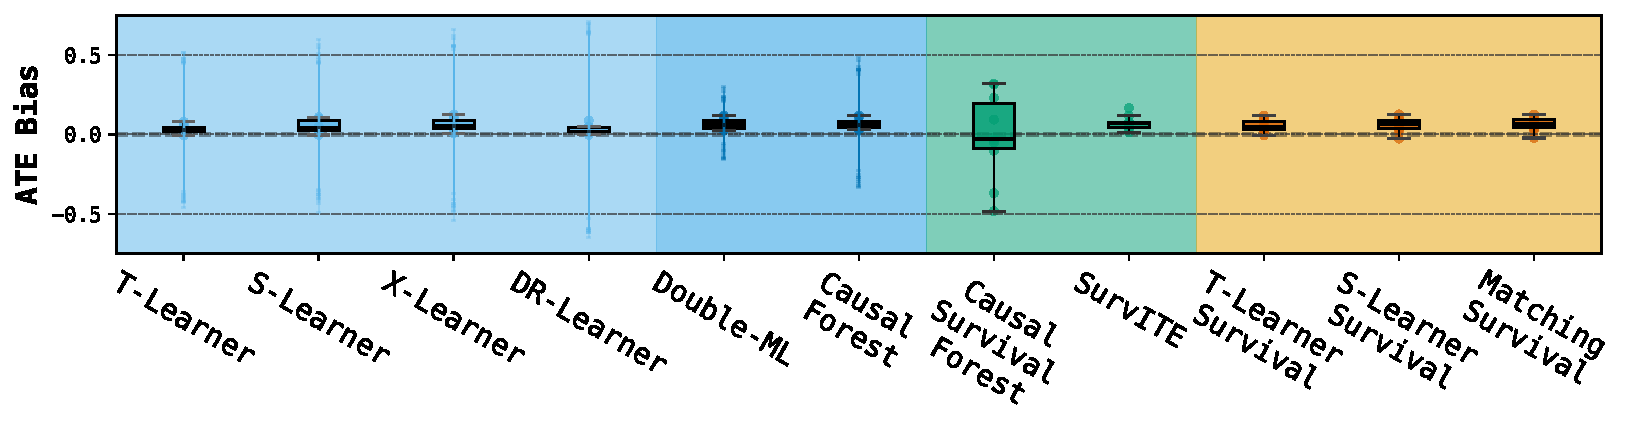
\includegraphics[width=\linewidth]{Appendices/appendix-ch04/images/figure_results_updated/ate_bias/Scenario_A_OBS-UConf_ate_bias.pdf}
        
    \end{minipage}}

    

    \subfloat[{RCT: \ChFourBlackCross, Ignorability: \ChFourGrayCheck, Positivity: \ChFourBlackCross, Ignorable Censoring: \ChFourGrayCheck}]{\begin{minipage}[t]{0.49\textwidth}
        \centering
        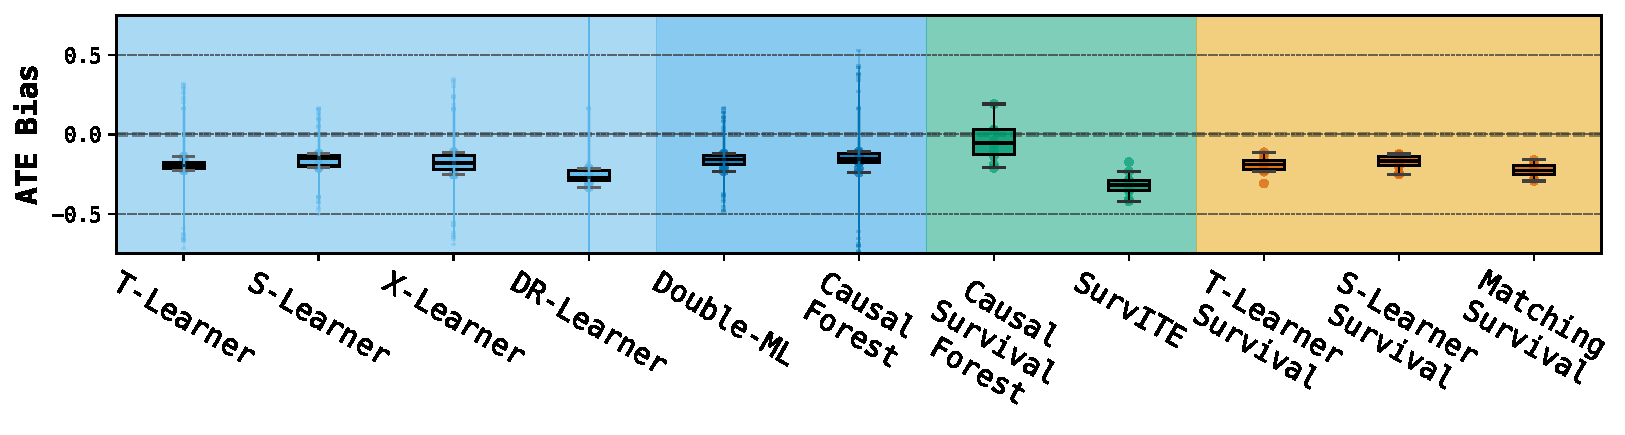
\includegraphics[width=\linewidth]{Appendices/appendix-ch04/images/figure_results_updated/ate_bias/Scenario_A_OBS-NoPos_ate_bias.pdf}
        
    \end{minipage}}
    \hfill
    \subfloat[{RCT: \ChFourBlackCross, Ignorability: \ChFourGrayCheck, Positivity: \ChFourGrayCheck, Ignorable Censoring: \ChFourBlackCross}]{\begin{minipage}[t]{0.49\textwidth}
        \centering
        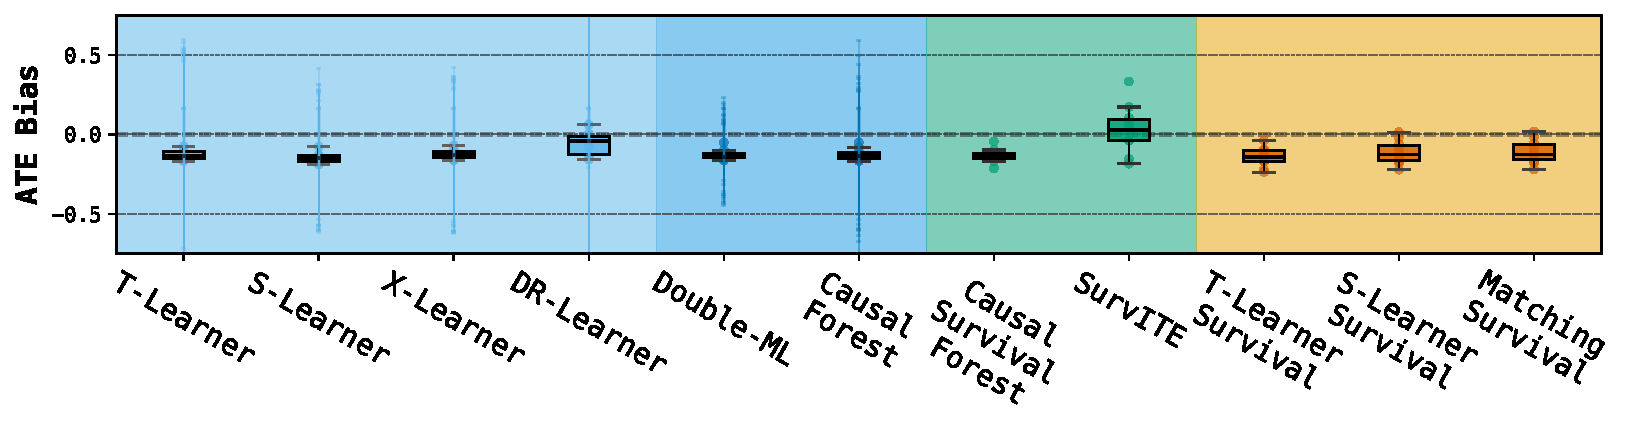
\includegraphics[width=\linewidth]{Appendices/appendix-ch04/images/figure_results_updated/ate_bias/Scenario_A_OBS-CPS-IC_ate_bias.pdf}
        
    \end{minipage}}

    

    \subfloat[{RCT: \ChFourBlackCross, Ignorability: \ChFourBlackCross, Positivity: \ChFourGrayCheck, Ignorable Censoring: \ChFourBlackCross}]{\begin{minipage}[t]{0.49\textwidth}
        \centering
        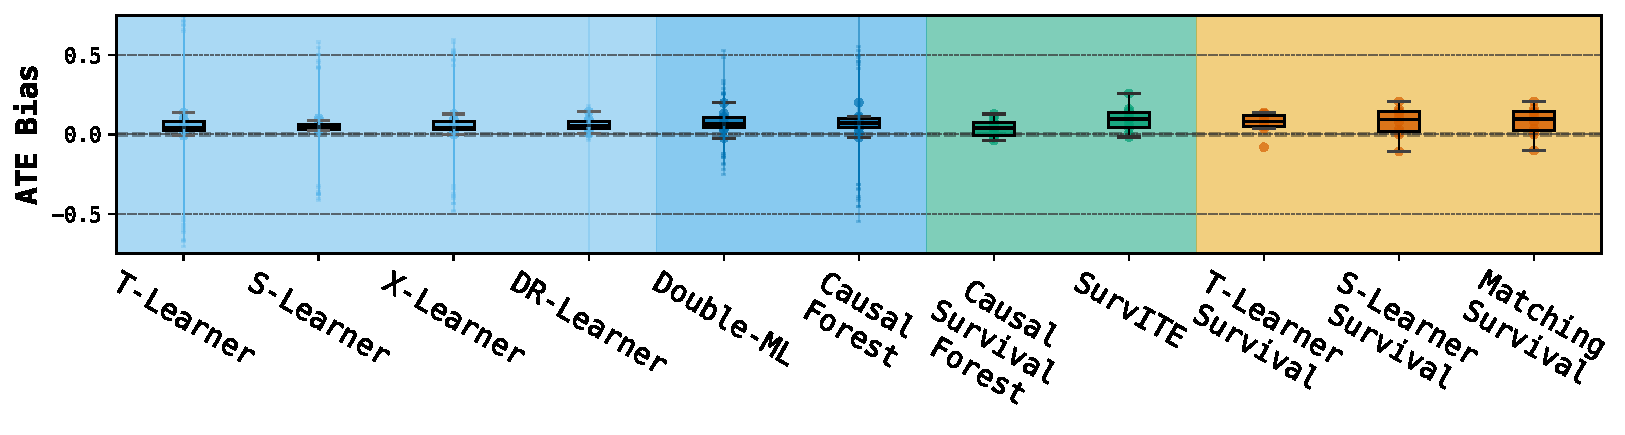
\includegraphics[width=\linewidth]{Appendices/appendix-ch04/images/figure_results_updated/ate_bias/Scenario_A_OBS-UConf-IC_ate_bias.pdf}
        
    \end{minipage}}
    \hfill
    \subfloat[{RCT: \ChFourBlackCross, Ignorability: \ChFourGrayCheck, Positivity: \ChFourBlackCross, Ignorable Censoring: \ChFourBlackCross}]{\begin{minipage}[t]{0.49\textwidth}
        \centering
        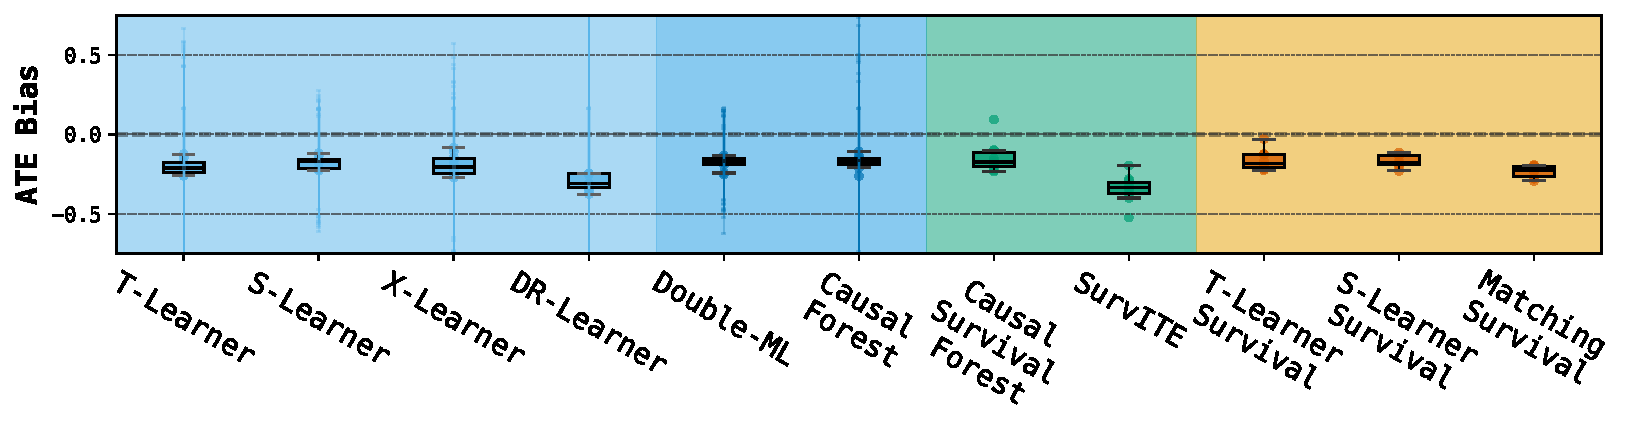
\includegraphics[width=\linewidth]{Appendices/appendix-ch04/images/figure_results_updated/ate_bias/Scenario_A_OBS-NoPos-IC_ate_bias.pdf}
        
    \end{minipage}}

                    \end{minipage}%
    }

    
    
}
\end{figure}

% 



% Secnario B

% !TeX root = ../../../main.tex
\begin{figure}[htbp]
\ChFourFloatContents{ch04:fig:ate_bias_grid_scenario_B}{\caption{ATE Bias across different experiments in Scenario \texttt{B}.}}{
    \centering

            \resizebox{0.95\textwidth}{!}{%
        \begin{minipage}{1\textwidth}

    \subfloat[{RCT: \ChFourGrayCheck (50\%), Ignorability: \ChFourGrayCheck, Positivity: \ChFourGrayCheck, Ign-Censoring: \ChFourGrayCheck}]{\begin{minipage}[t]{0.49\textwidth}
        \centering
        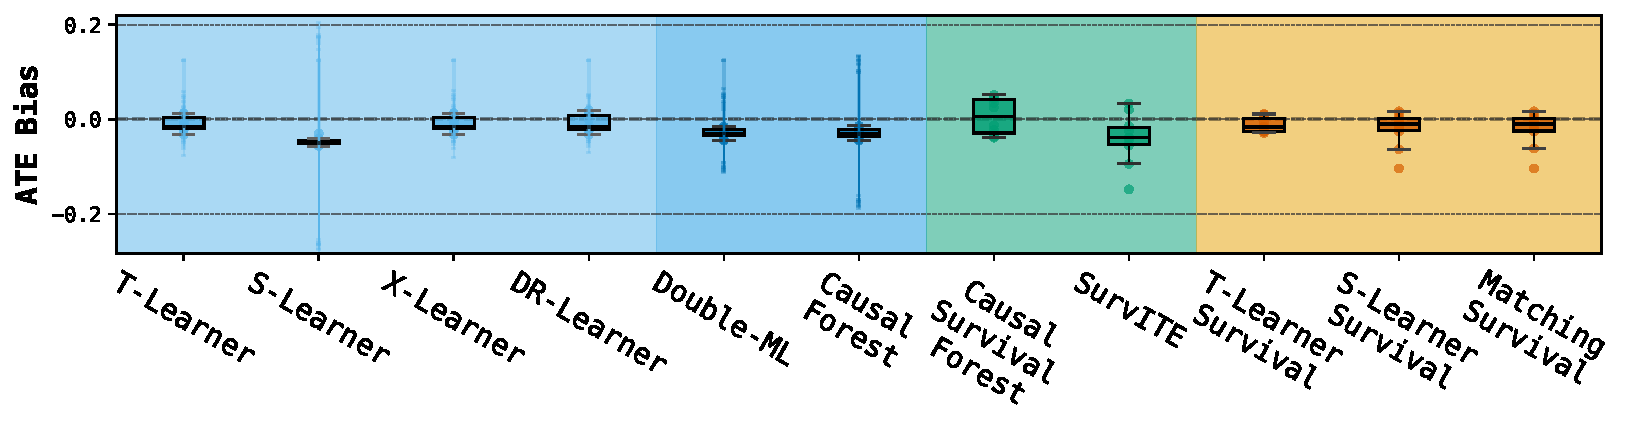
\includegraphics[width=\linewidth]{Appendices/appendix-ch04/images/figure_results_updated/ate_bias/Scenario_B_RCT-50_ate_bias.pdf}
        
    \end{minipage}}
    \hfill
    \subfloat[{RCT: \ChFourGrayCheck (5\%), Ignorability: \ChFourGrayCheck, Positivity: \ChFourGrayCheck, Ign-Censoring: \ChFourGrayCheck}]{\begin{minipage}[t]{0.49\textwidth}
        \centering
        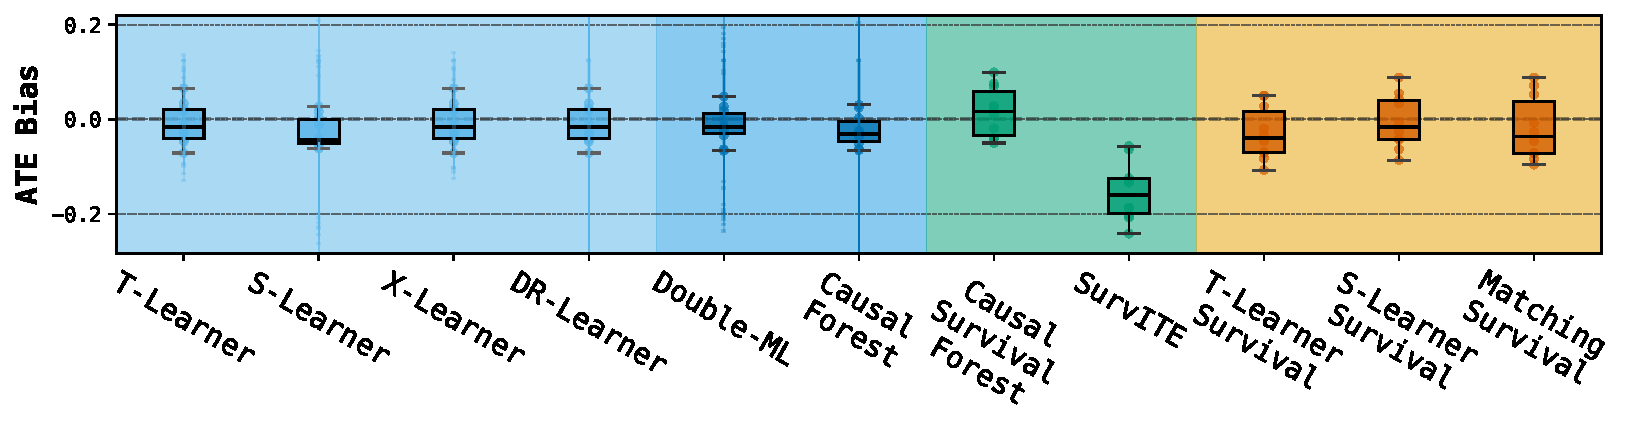
\includegraphics[width=\linewidth]{Appendices/appendix-ch04/images/figure_results_updated/ate_bias/Scenario_B_RCT-5_ate_bias.pdf}
        
    \end{minipage}}

    

    \subfloat[{RCT: \ChFourBlackCross, Ignorability: \ChFourGrayCheck, Positivity: \ChFourGrayCheck, Ignorable Censoring: \ChFourGrayCheck}]{\begin{minipage}[t]{0.49\textwidth}
        \centering
        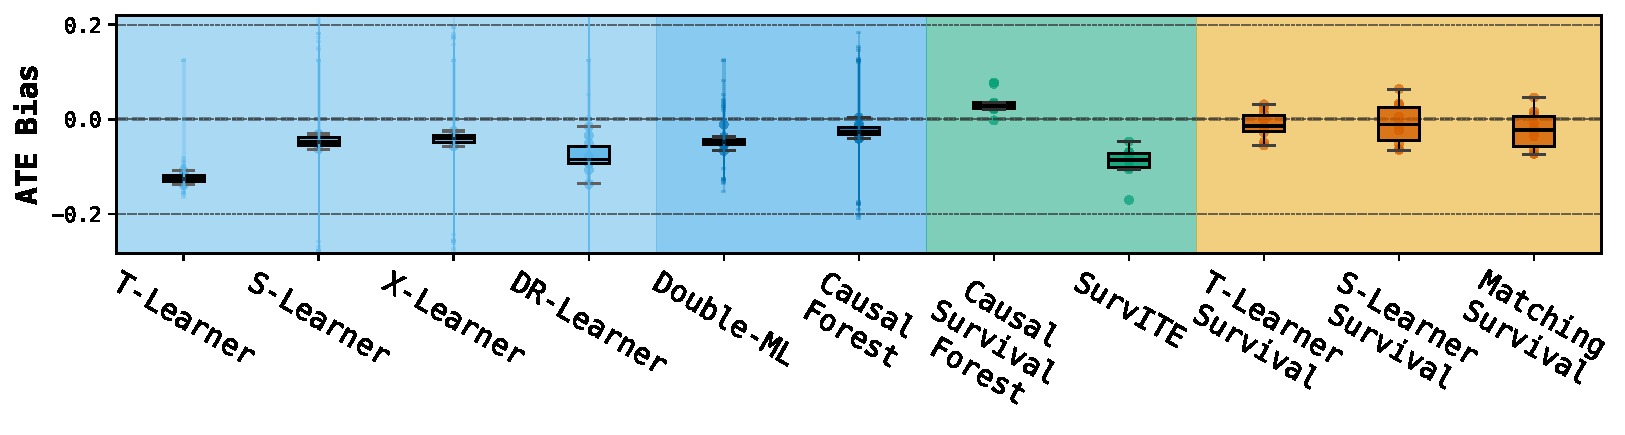
\includegraphics[width=\linewidth]{Appendices/appendix-ch04/images/figure_results_updated/ate_bias/Scenario_B_OBS-CPS_ate_bias.pdf}
        
    \end{minipage}}
    \hfill
    \subfloat[{RCT: \ChFourBlackCross, Ignorability: \ChFourBlackCross, Positivity: \ChFourGrayCheck, Ignorable Censoring: \ChFourGrayCheck}]{\begin{minipage}[t]{0.49\textwidth}
        \centering
        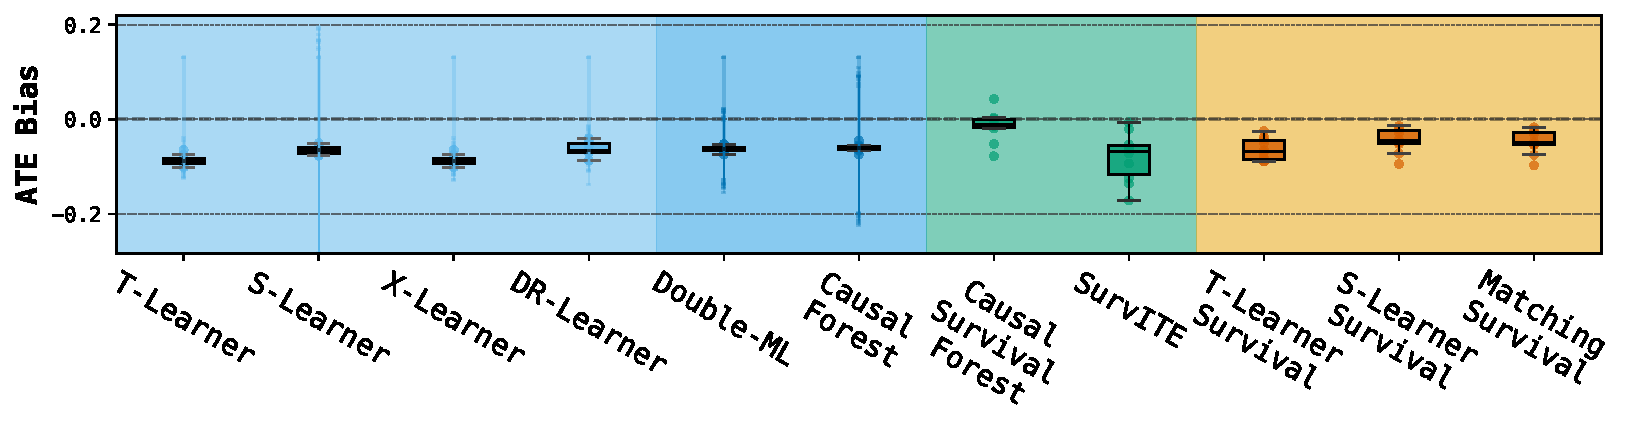
\includegraphics[width=\linewidth]{Appendices/appendix-ch04/images/figure_results_updated/ate_bias/Scenario_B_OBS-UConf_ate_bias.pdf}
        
    \end{minipage}}

    

    \subfloat[{RCT: \ChFourBlackCross, Ignorability: \ChFourGrayCheck, Positivity: \ChFourBlackCross, Ignorable Censoring: \ChFourGrayCheck}]{\begin{minipage}[t]{0.49\textwidth}
        \centering
        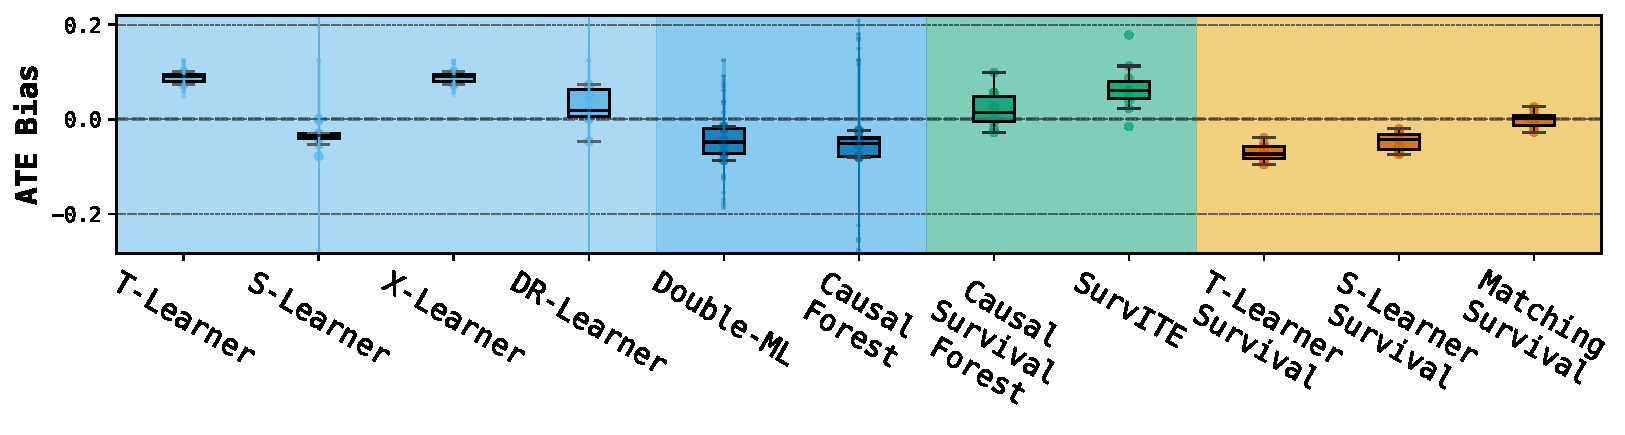
\includegraphics[width=\linewidth]{Appendices/appendix-ch04/images/figure_results_updated/ate_bias/Scenario_B_OBS-NoPos_ate_bias.pdf}
        
    \end{minipage}}
    \hfill
    \subfloat[{RCT: \ChFourBlackCross, Ignorability: \ChFourGrayCheck, Positivity: \ChFourGrayCheck, Ignorable Censoring: \ChFourBlackCross}]{\begin{minipage}[t]{0.49\textwidth}
        \centering
        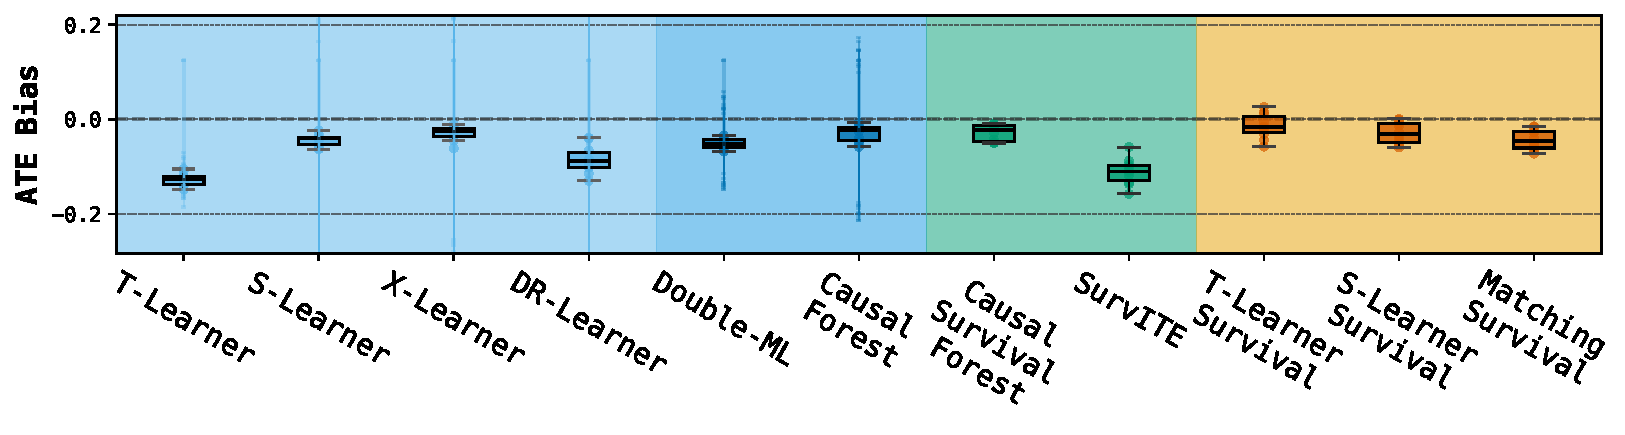
\includegraphics[width=\linewidth]{Appendices/appendix-ch04/images/figure_results_updated/ate_bias/Scenario_B_OBS-CPS-IC_ate_bias.pdf}
        
    \end{minipage}}

    

    \subfloat[{RCT: \ChFourBlackCross, Ignorability: \ChFourBlackCross, Positivity: \ChFourGrayCheck, Ignorable Censoring: \ChFourBlackCross}]{\begin{minipage}[t]{0.49\textwidth}
        \centering
        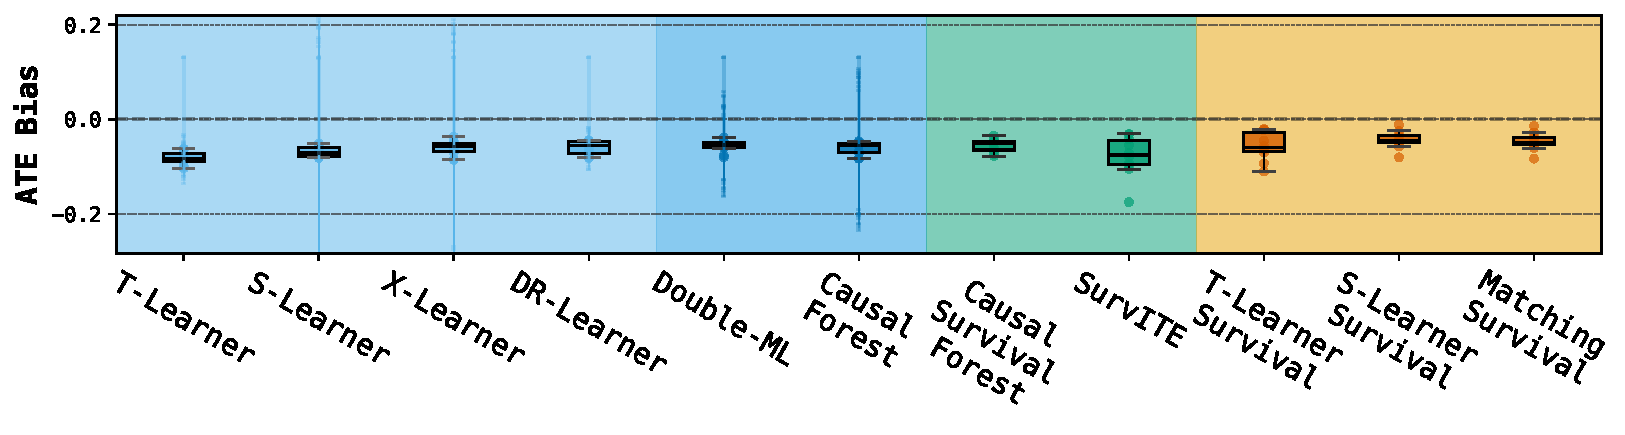
\includegraphics[width=\linewidth]{Appendices/appendix-ch04/images/figure_results_updated/ate_bias/Scenario_B_OBS-UConf-IC_ate_bias.pdf}
        
    \end{minipage}}
    \hfill
    \subfloat[{RCT: \ChFourBlackCross, Ignorability: \ChFourGrayCheck, Positivity: \ChFourBlackCross, Ignorable Censoring: \ChFourBlackCross}]{\begin{minipage}[t]{0.49\textwidth}
        \centering
        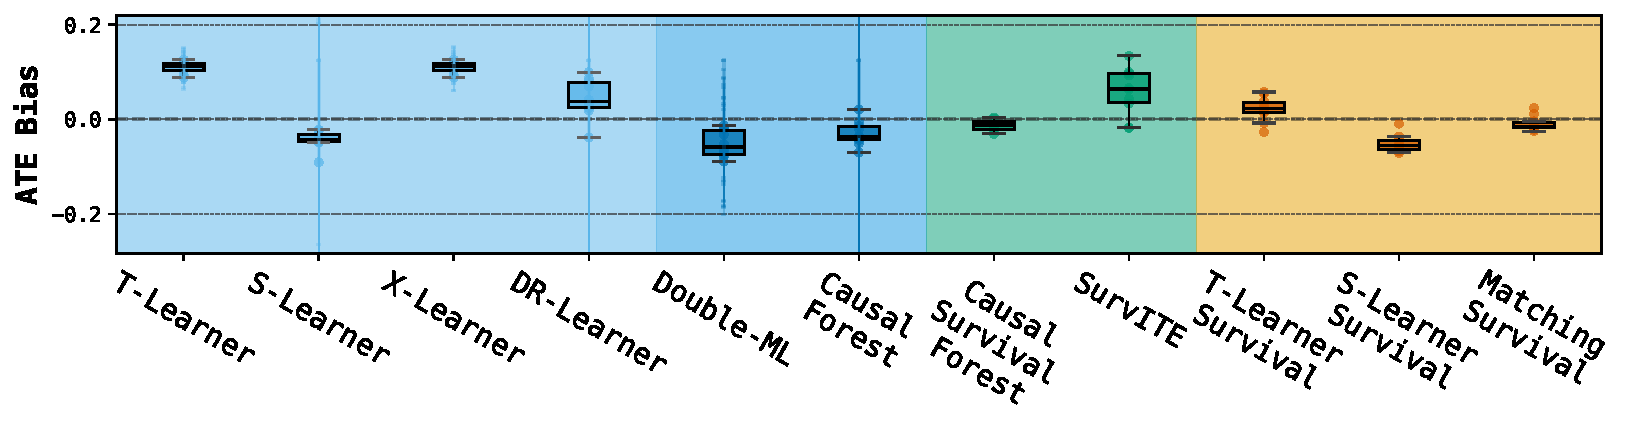
\includegraphics[width=\linewidth]{Appendices/appendix-ch04/images/figure_results_updated/ate_bias/Scenario_B_OBS-NoPos-IC_ate_bias.pdf}
        
    \end{minipage}}

                    \end{minipage}%
    }

    
    
}
\end{figure}


% 

% Secnario C

% !TeX root = ../../../main.tex
\begin{figure}[htbp]
\ChFourFloatContents{ch04:fig:ate_bias_grid_scenario_C}{\caption{ATE Bias across different experiments in Scenario \texttt{C}.}}{
    \centering

            \resizebox{0.95\textwidth}{!}{%
        \begin{minipage}{1\textwidth}

    \subfloat[{RCT: \ChFourGrayCheck (50\%), Ignorability: \ChFourGrayCheck, Positivity: \ChFourGrayCheck, Ign-Censoring: \ChFourGrayCheck}]{\begin{minipage}[t]{0.49\textwidth}
        \centering
        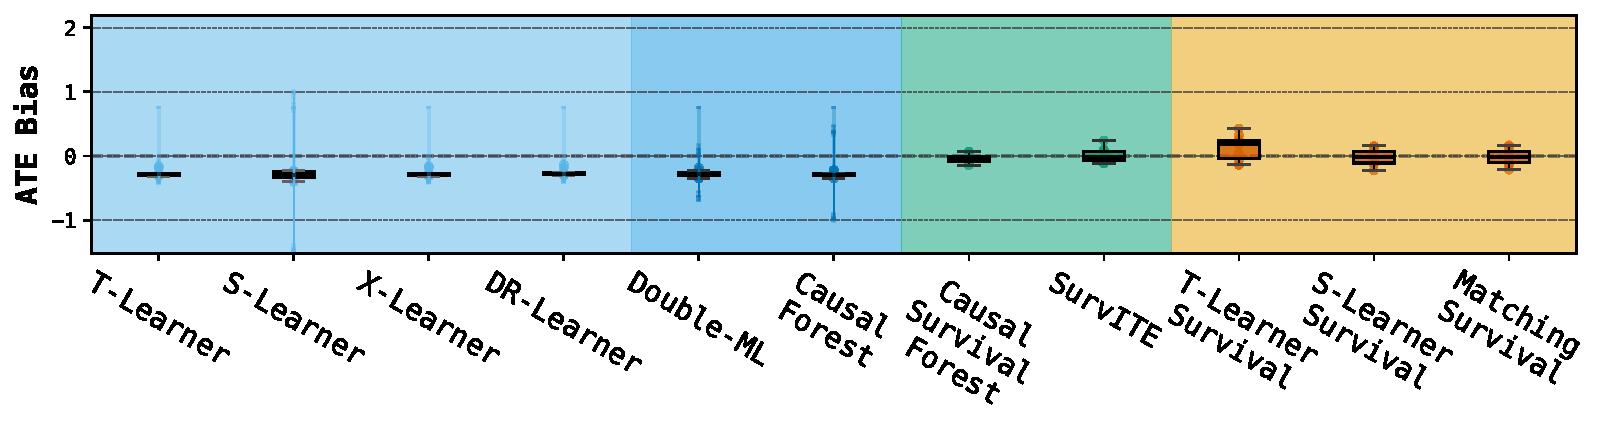
\includegraphics[width=\linewidth]{Appendices/appendix-ch04/images/figure_results_updated/ate_bias/Scenario_C_RCT-50_ate_bias.pdf}
        
    \end{minipage}}
    \hfill
    \subfloat[{RCT: \ChFourGrayCheck (5\%), Ignorability: \ChFourGrayCheck, Positivity: \ChFourGrayCheck, Ign-Censoring: \ChFourGrayCheck}]{\begin{minipage}[t]{0.49\textwidth}
        \centering
        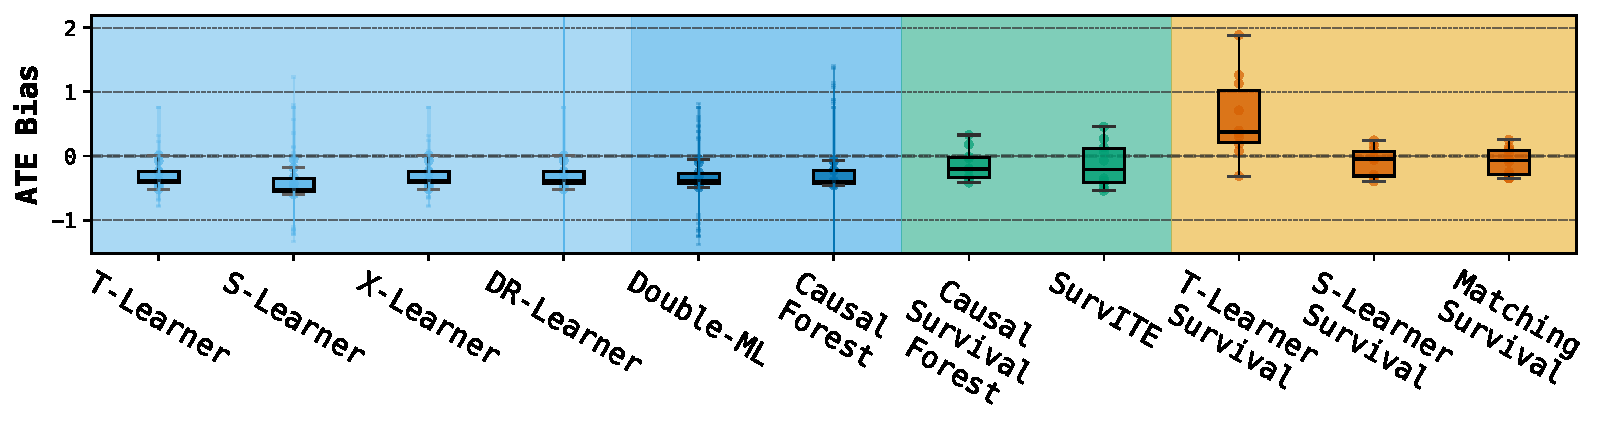
\includegraphics[width=\linewidth]{Appendices/appendix-ch04/images/figure_results_updated/ate_bias/Scenario_C_RCT-5_ate_bias.pdf}
        
    \end{minipage}}

    

    \subfloat[{RCT: \ChFourBlackCross, Ignorability: \ChFourGrayCheck, Positivity: \ChFourGrayCheck, Ignorable Censoring: \ChFourGrayCheck}]{\begin{minipage}[t]{0.49\textwidth}
        \centering
        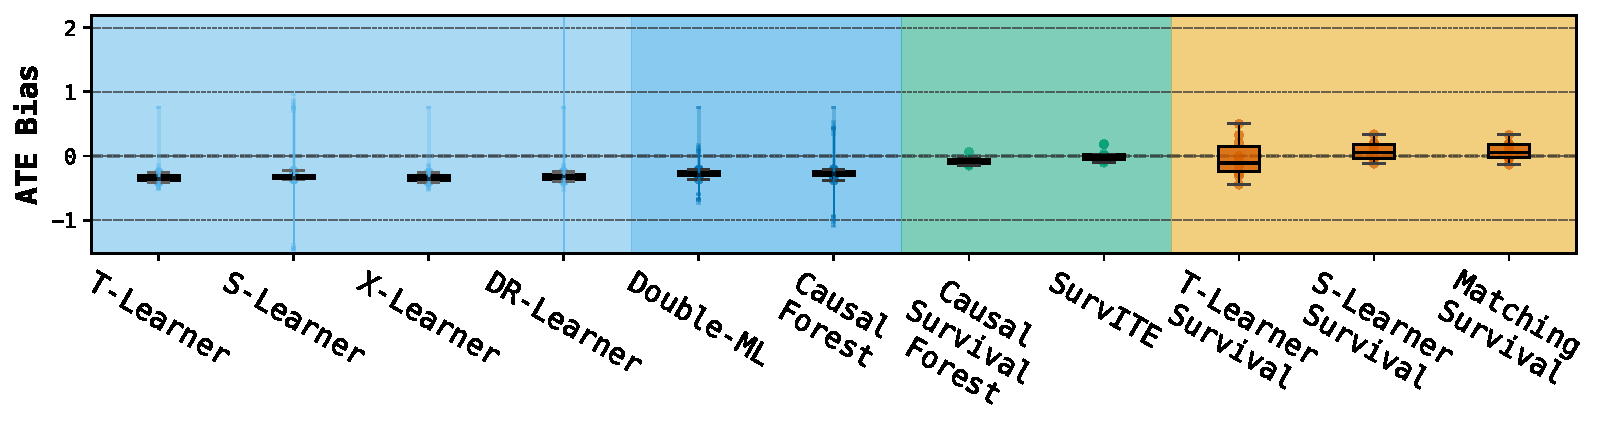
\includegraphics[width=\linewidth]{Appendices/appendix-ch04/images/figure_results_updated/ate_bias/Scenario_C_OBS-CPS_ate_bias.pdf}
        
    \end{minipage}}
    \hfill
    \subfloat[{RCT: \ChFourBlackCross, Ignorability: \ChFourBlackCross, Positivity: \ChFourGrayCheck, Ignorable Censoring: \ChFourGrayCheck}]{\begin{minipage}[t]{0.49\textwidth}
        \centering
        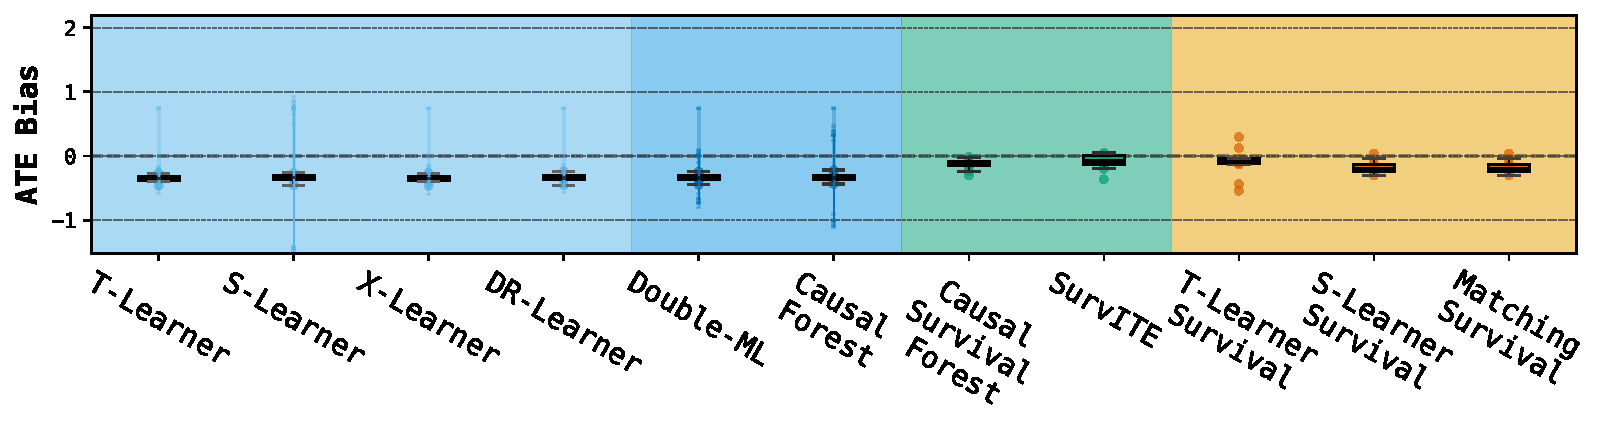
\includegraphics[width=\linewidth]{Appendices/appendix-ch04/images/figure_results_updated/ate_bias/Scenario_C_OBS-UConf_ate_bias.pdf}
        
    \end{minipage}}

    

    \subfloat[{RCT: \ChFourBlackCross, Ignorability: \ChFourGrayCheck, Positivity: \ChFourBlackCross, Ignorable Censoring: \ChFourGrayCheck}]{\begin{minipage}[t]{0.49\textwidth}
        \centering
        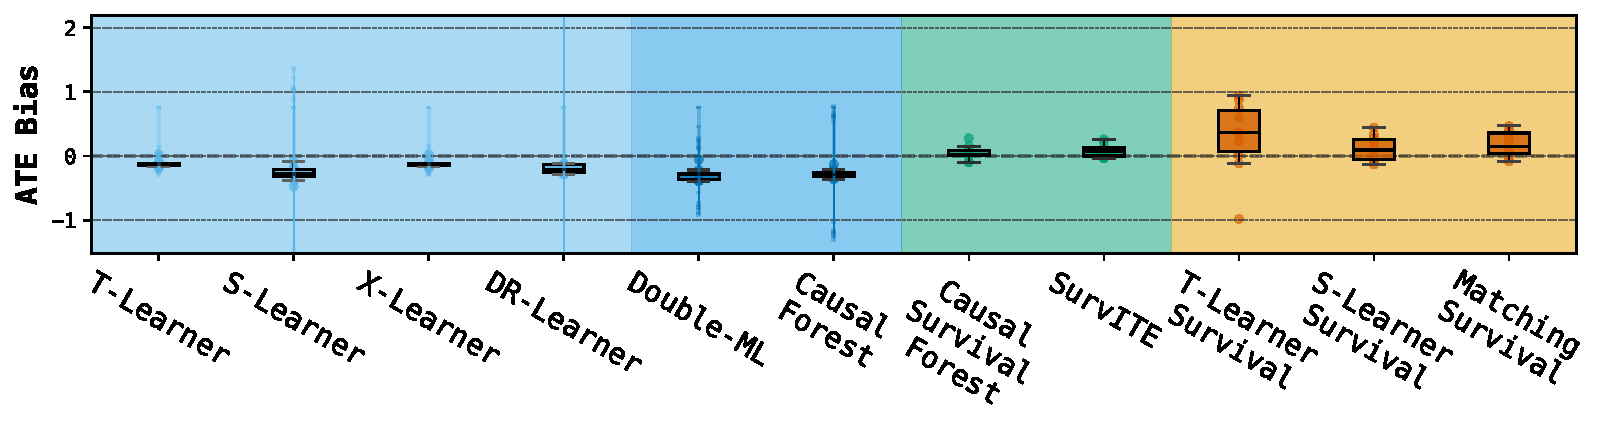
\includegraphics[width=\linewidth]{Appendices/appendix-ch04/images/figure_results_updated/ate_bias/Scenario_C_OBS-NoPos_ate_bias.pdf}
        
    \end{minipage}}
    \hfill
    \subfloat[{RCT: \ChFourBlackCross, Ignorability: \ChFourGrayCheck, Positivity: \ChFourGrayCheck, Ignorable Censoring: \ChFourBlackCross}]{\begin{minipage}[t]{0.49\textwidth}
        \centering
        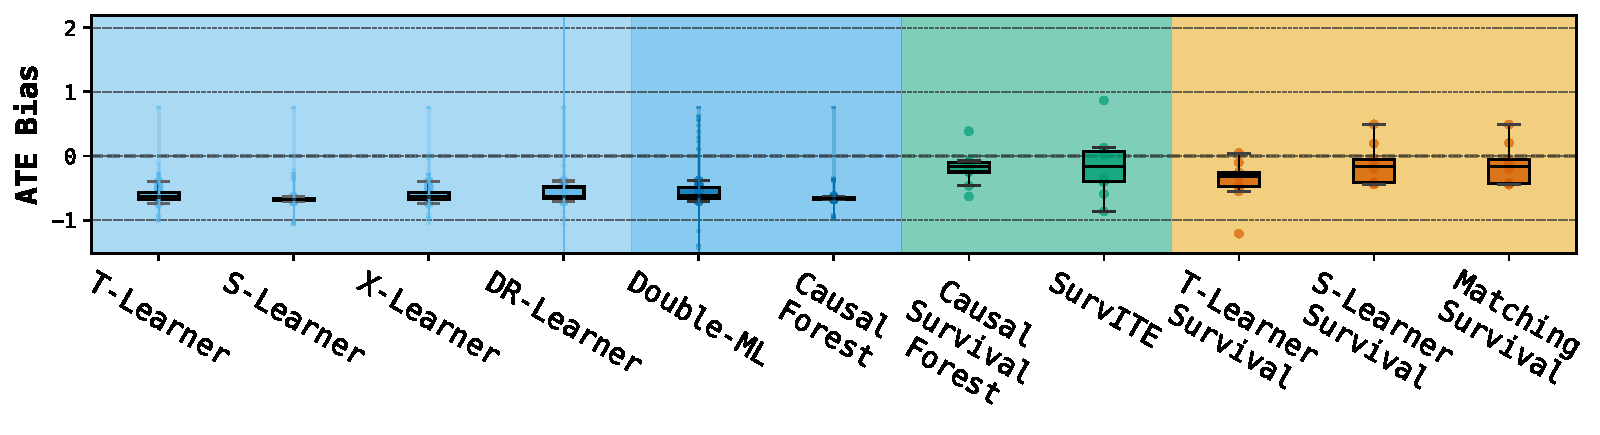
\includegraphics[width=\linewidth]{Appendices/appendix-ch04/images/figure_results_updated/ate_bias/Scenario_C_OBS-CPS-IC_ate_bias.pdf}
        
    \end{minipage}}

    

    \subfloat[{RCT: \ChFourBlackCross, Ignorability: \ChFourBlackCross, Positivity: \ChFourGrayCheck, Ignorable Censoring: \ChFourBlackCross}]{\begin{minipage}[t]{0.49\textwidth}
        \centering
        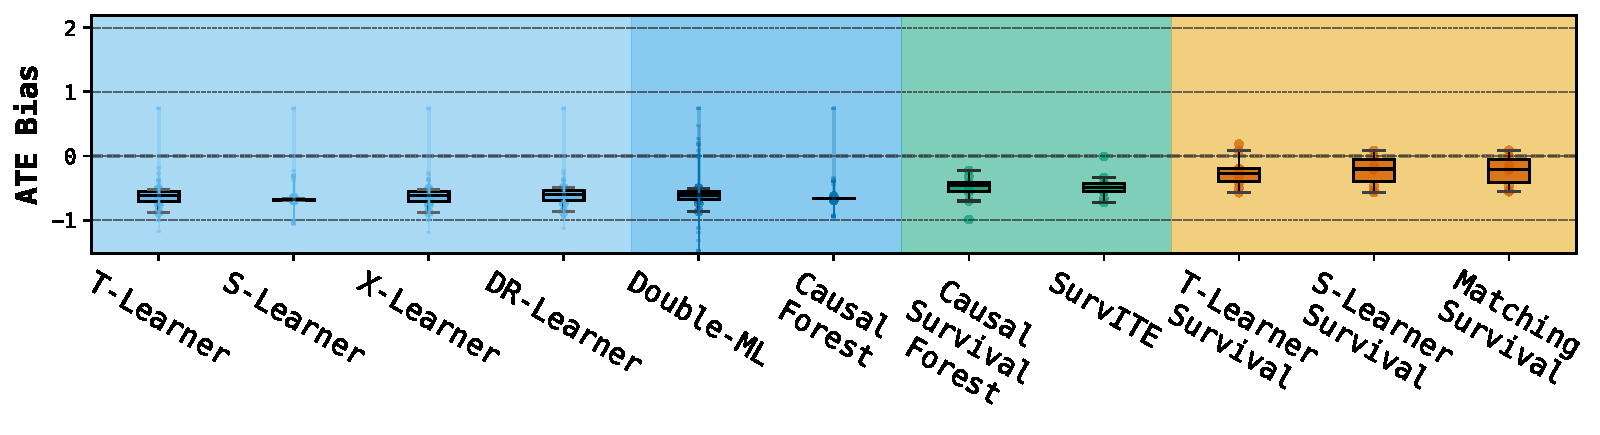
\includegraphics[width=\linewidth]{Appendices/appendix-ch04/images/figure_results_updated/ate_bias/Scenario_C_OBS-UConf-IC_ate_bias.pdf}
        
    \end{minipage}}
    \hfill
    \subfloat[{RCT: \ChFourBlackCross, Ignorability: \ChFourGrayCheck, Positivity: \ChFourBlackCross, Ignorable Censoring: \ChFourBlackCross}]{\begin{minipage}[t]{0.49\textwidth}
        \centering
        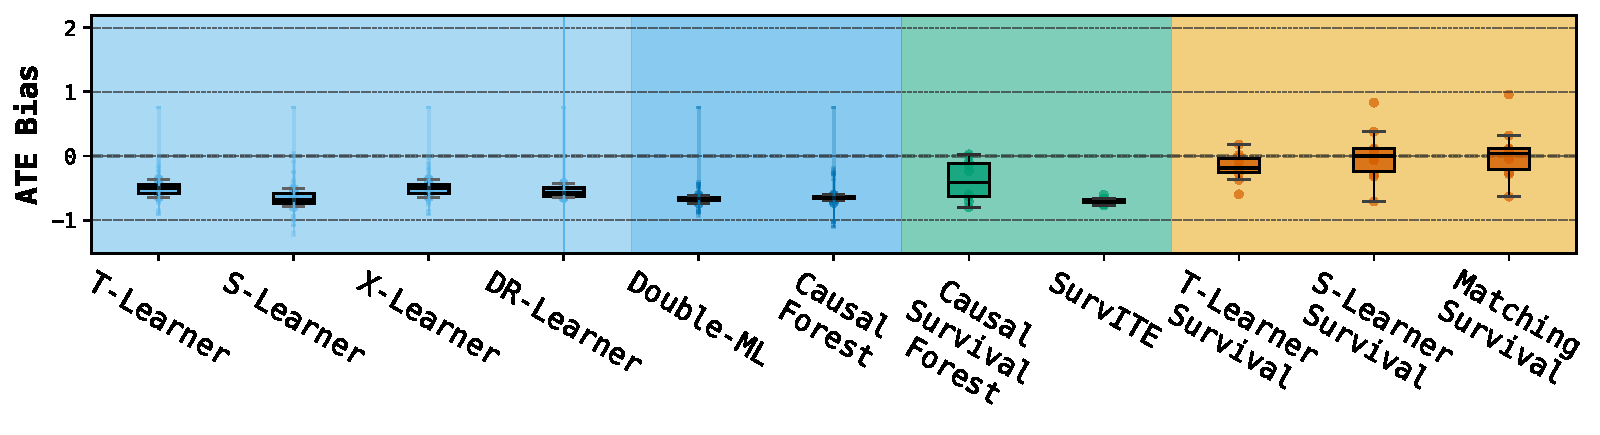
\includegraphics[width=\linewidth]{Appendices/appendix-ch04/images/figure_results_updated/ate_bias/Scenario_C_OBS-NoPos-IC_ate_bias.pdf}
        
    \end{minipage}}

                    \end{minipage}%
    }

    
    
}
\end{figure}


% 



% Scenario D

% !TeX root = ../../../main.tex
\begin{figure}[htbp]
\ChFourFloatContents{ch04:fig:ate_bias_grid_scenario_D}{\caption{ATE Bias across different experiments in Scenario \texttt{D}.}}{
    \centering

            \resizebox{0.95\textwidth}{!}{%
        \begin{minipage}{1\textwidth}

    \subfloat[{RCT: \ChFourGrayCheck (50\%), Ignorability: \ChFourGrayCheck, Positivity: \ChFourGrayCheck, Ign-Censoring: \ChFourGrayCheck}]{\begin{minipage}[t]{0.49\textwidth}
        \centering
        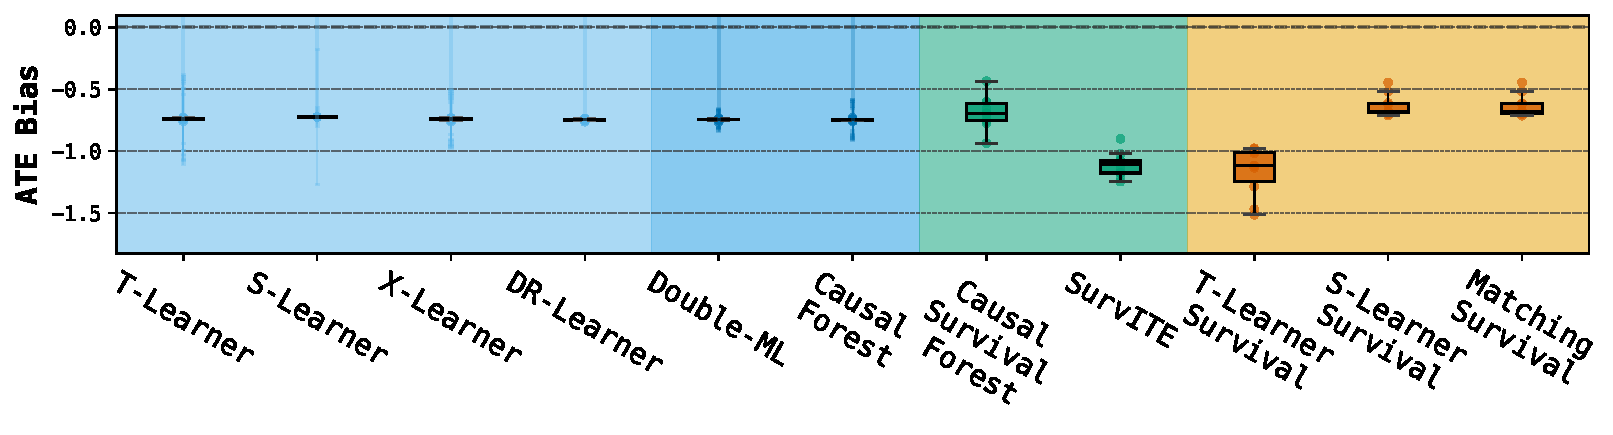
\includegraphics[width=\linewidth]{Appendices/appendix-ch04/images/figure_results_updated/ate_bias/Scenario_D_RCT-50_ate_bias.pdf}
        
    \end{minipage}}
    \hfill
    \subfloat[{RCT: \ChFourGrayCheck (5\%), Ignorability: \ChFourGrayCheck, Positivity: \ChFourGrayCheck, Ign-Censoring: \ChFourGrayCheck}]{\begin{minipage}[t]{0.49\textwidth}
        \centering
        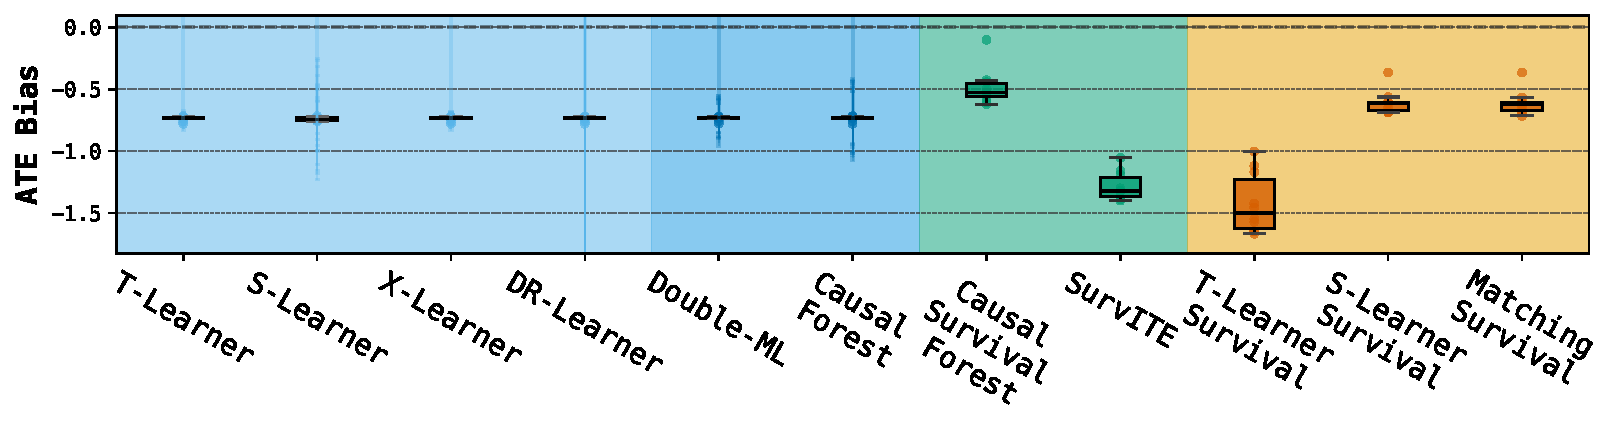
\includegraphics[width=\linewidth]{Appendices/appendix-ch04/images/figure_results_updated/ate_bias/Scenario_D_RCT-5_ate_bias.pdf}
        
    \end{minipage}}

    

    \subfloat[{RCT: \ChFourBlackCross, Ignorability: \ChFourGrayCheck, Positivity: \ChFourGrayCheck, Ignorable Censoring: \ChFourGrayCheck}]{\begin{minipage}[t]{0.49\textwidth}
        \centering
        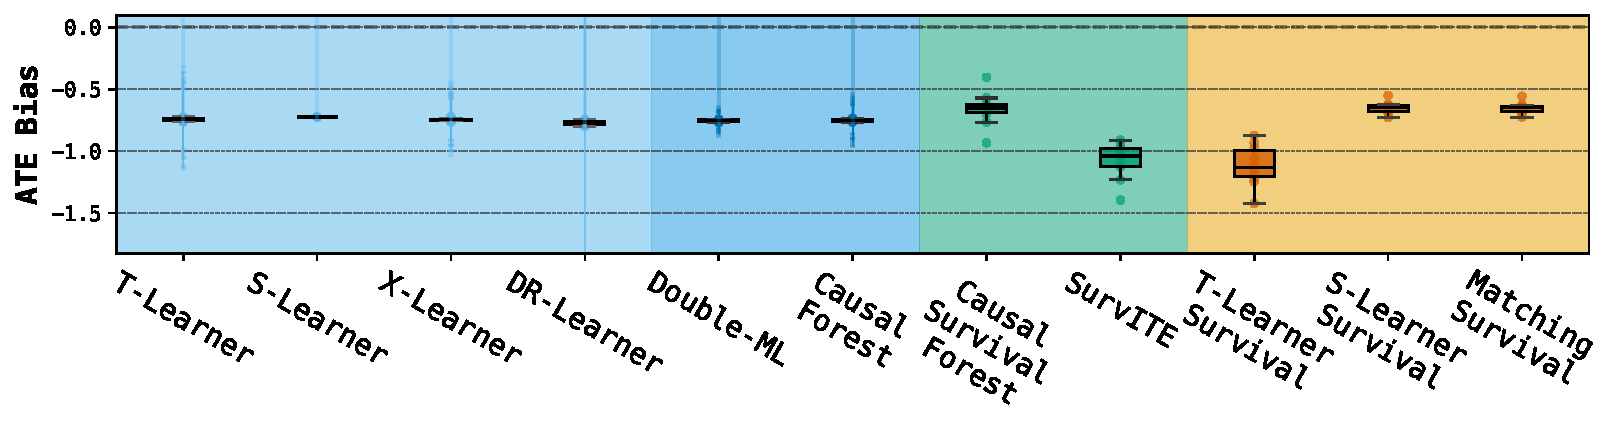
\includegraphics[width=\linewidth]{Appendices/appendix-ch04/images/figure_results_updated/ate_bias/Scenario_D_OBS-CPS_ate_bias.pdf}
        
    \end{minipage}}
    \hfill
    \subfloat[{RCT: \ChFourBlackCross, Ignorability: \ChFourBlackCross, Positivity: \ChFourGrayCheck, Ignorable Censoring: \ChFourGrayCheck}]{\begin{minipage}[t]{0.49\textwidth}
        \centering
        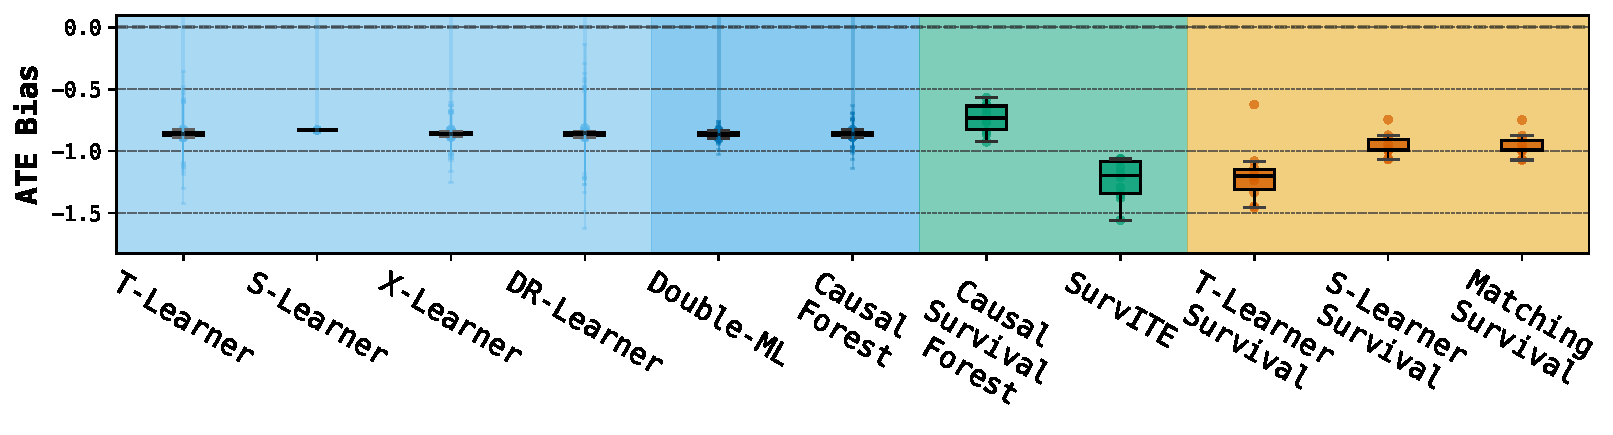
\includegraphics[width=\linewidth]{Appendices/appendix-ch04/images/figure_results_updated/ate_bias/Scenario_D_OBS-UConf_ate_bias.pdf}
        
    \end{minipage}}

    

    \subfloat[{RCT: \ChFourBlackCross, Ignorability: \ChFourGrayCheck, Positivity: \ChFourBlackCross, Ignorable Censoring: \ChFourGrayCheck}]{\begin{minipage}[t]{0.49\textwidth}
        \centering
        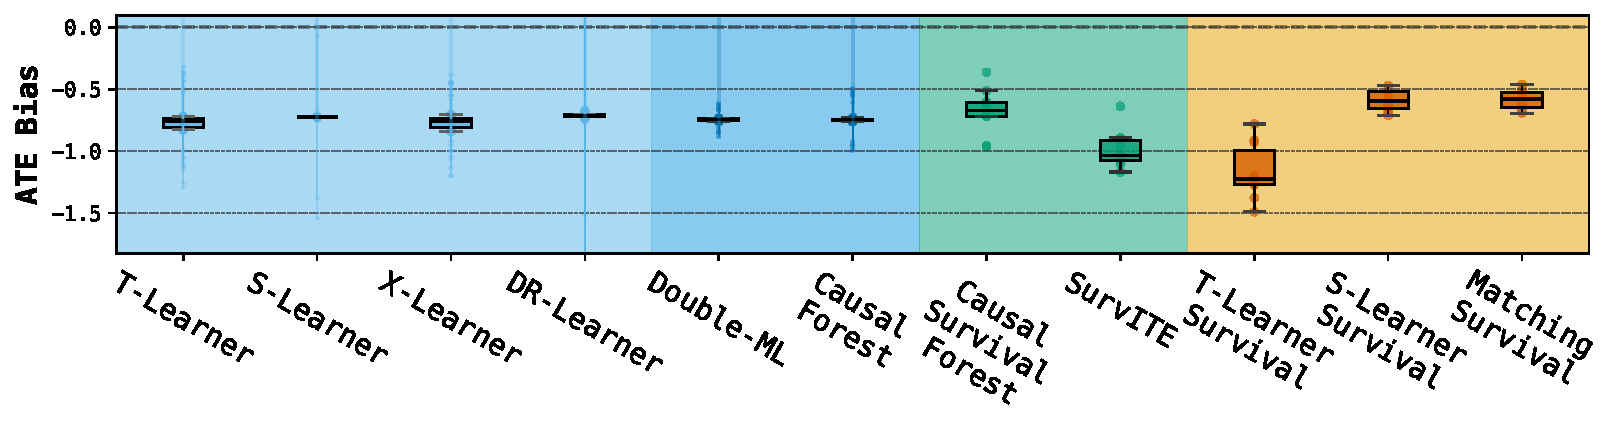
\includegraphics[width=\linewidth]{Appendices/appendix-ch04/images/figure_results_updated/ate_bias/Scenario_D_OBS-NoPos_ate_bias.pdf}
        
    \end{minipage}}
    \hfill
    \subfloat[{RCT: \ChFourBlackCross, Ignorability: \ChFourGrayCheck, Positivity: \ChFourGrayCheck, Ignorable Censoring: \ChFourBlackCross}]{\begin{minipage}[t]{0.49\textwidth}
        \centering
        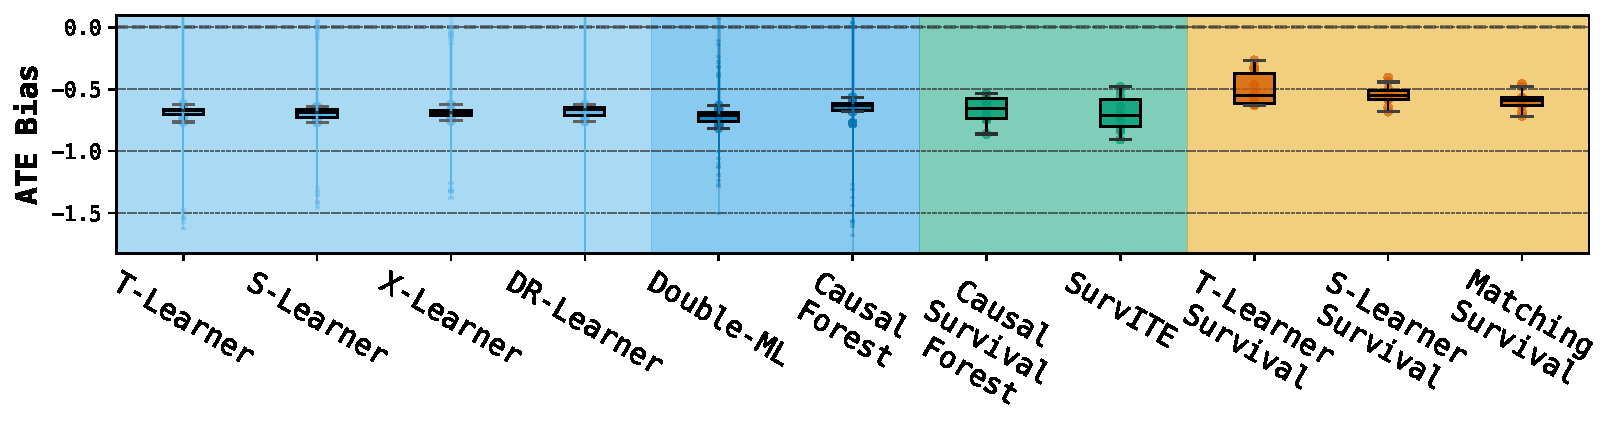
\includegraphics[width=\linewidth]{Appendices/appendix-ch04/images/figure_results_updated/ate_bias/Scenario_D_OBS-CPS-IC_ate_bias.pdf}
        
    \end{minipage}}

    

    \subfloat[{RCT: \ChFourBlackCross, Ignorability: \ChFourBlackCross, Positivity: \ChFourGrayCheck, Ignorable Censoring: \ChFourBlackCross}]{\begin{minipage}[t]{0.49\textwidth}
        \centering
        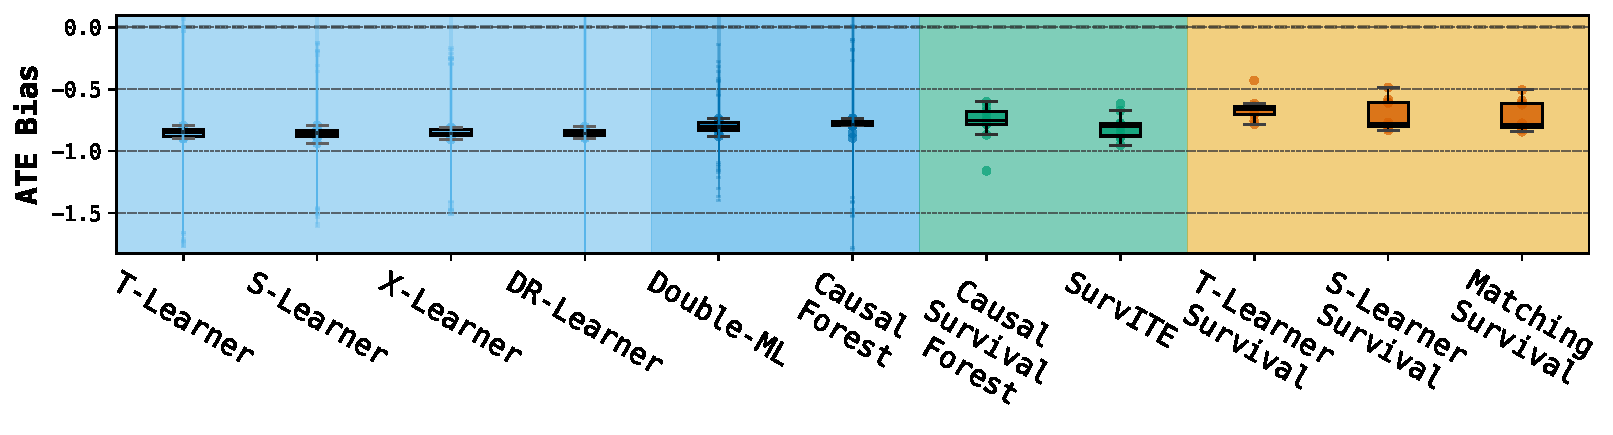
\includegraphics[width=\linewidth]{Appendices/appendix-ch04/images/figure_results_updated/ate_bias/Scenario_D_OBS-UConf-IC_ate_bias.pdf}
        
    \end{minipage}}
    \hfill
    \subfloat[{RCT: \ChFourBlackCross, Ignorability: \ChFourGrayCheck, Positivity: \ChFourBlackCross, Ignorable Censoring: \ChFourBlackCross}]{\begin{minipage}[t]{0.49\textwidth}
        \centering
        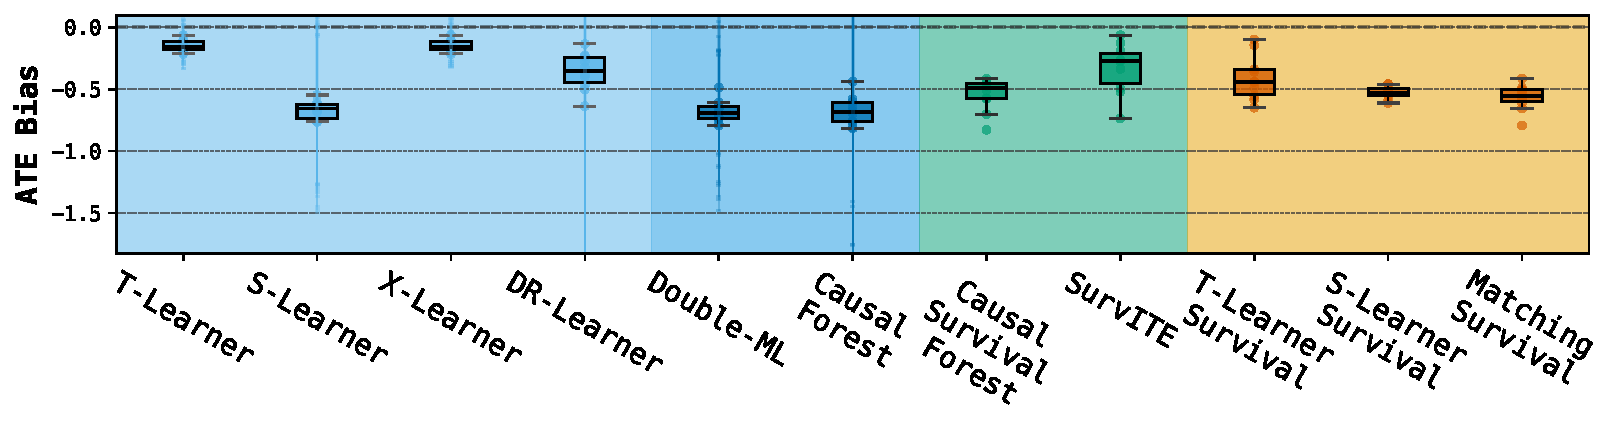
\includegraphics[width=\linewidth]{Appendices/appendix-ch04/images/figure_results_updated/ate_bias/Scenario_D_OBS-NoPos-IC_ate_bias.pdf}
        
    \end{minipage}}

                    \end{minipage}%
    }

    
    
}
\end{figure}



% 

% Secnario E

% !TeX root = ../../../main.tex
\begin{figure}[htbp]
\ChFourFloatContents{ch04:fig:ate_bias_grid_scenario_E}{\caption{ATE Bias across different experiments in Scenario \texttt{E}.}}{
    \centering

            \resizebox{0.95\textwidth}{!}{%
        \begin{minipage}{1\textwidth}

    \subfloat[{RCT: \ChFourGrayCheck (50\%), Ignorability: \ChFourGrayCheck, Positivity: \ChFourGrayCheck, Ign-Censoring: \ChFourGrayCheck}]{\begin{minipage}[t]{0.49\textwidth}
        \centering
        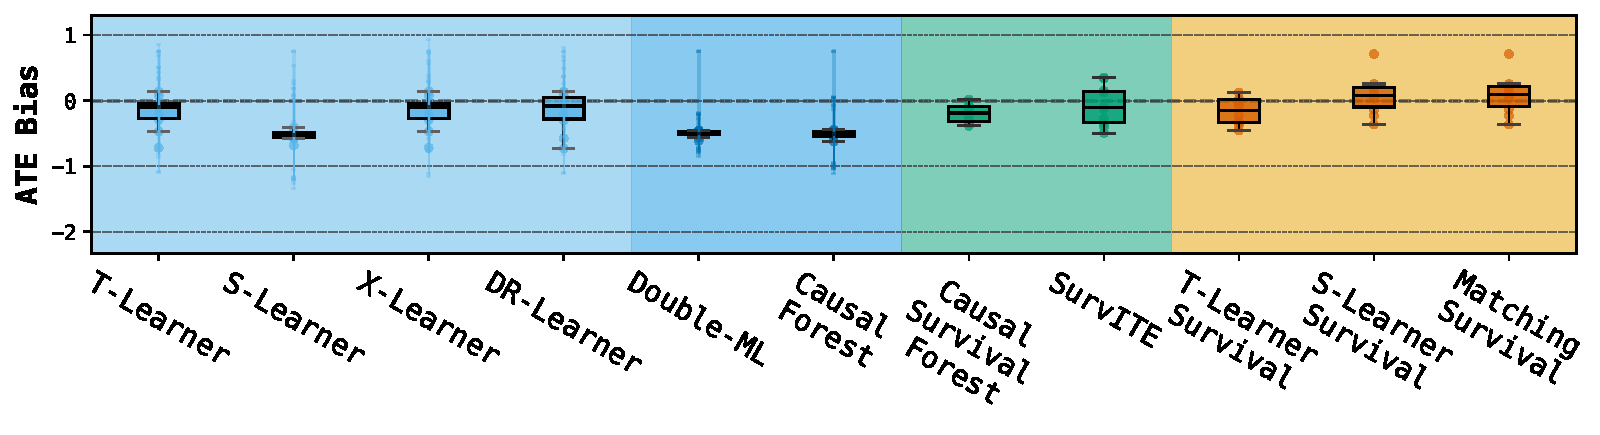
\includegraphics[width=\linewidth]{Appendices/appendix-ch04/images/figure_results_updated/ate_bias/Scenario_E_RCT-50_ate_bias.pdf}
        
    \end{minipage}}
    \hfill
    \subfloat[{RCT: \ChFourGrayCheck (5\%), Ignorability: \ChFourGrayCheck, Positivity: \ChFourGrayCheck, Ign-Censoring: \ChFourGrayCheck}]{\begin{minipage}[t]{0.49\textwidth}
        \centering
        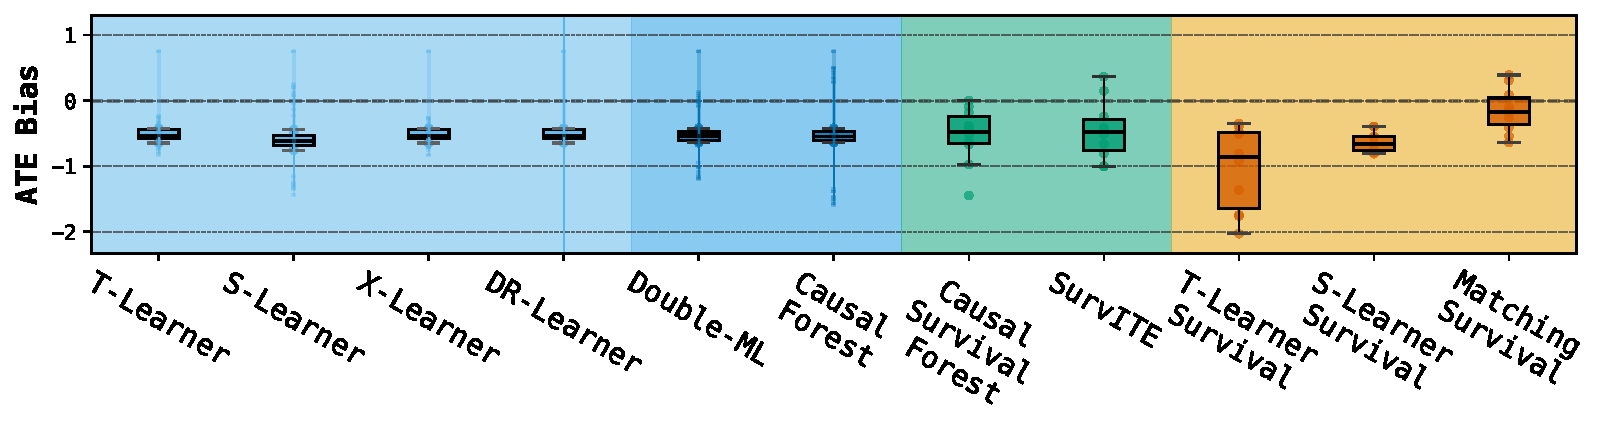
\includegraphics[width=\linewidth]{Appendices/appendix-ch04/images/figure_results_updated/ate_bias/Scenario_E_RCT-5_ate_bias.pdf}
        
    \end{minipage}}

    

    \subfloat[{RCT: \ChFourBlackCross, Ignorability: \ChFourGrayCheck, Positivity: \ChFourGrayCheck, Ignorable Censoring: \ChFourGrayCheck}]{\begin{minipage}[t]{0.49\textwidth}
        \centering
        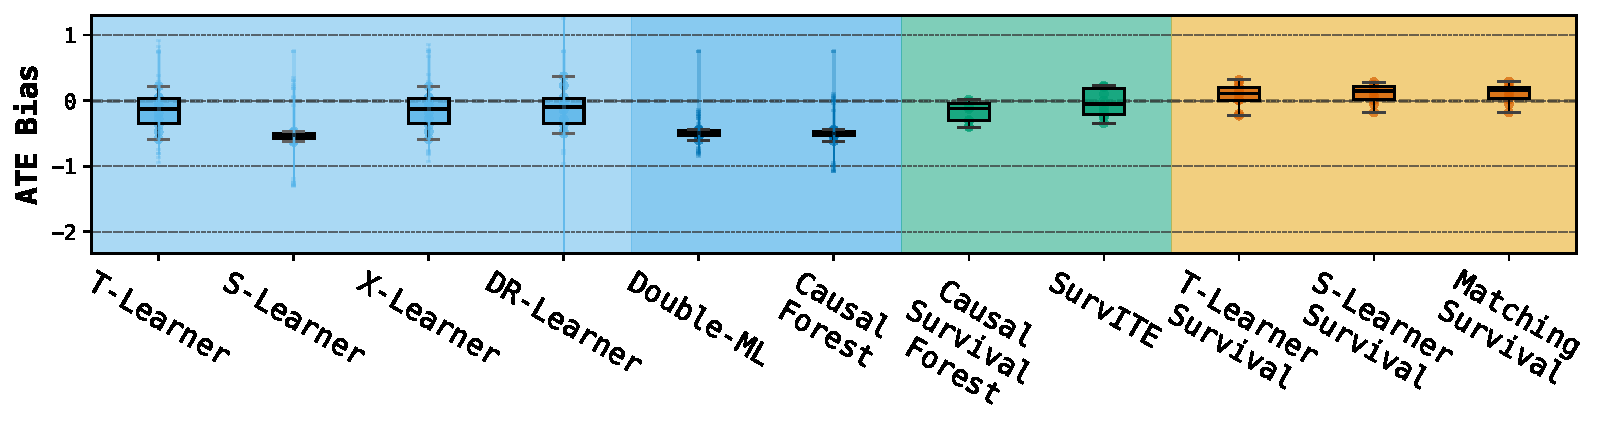
\includegraphics[width=\linewidth]{Appendices/appendix-ch04/images/figure_results_updated/ate_bias/Scenario_E_OBS-CPS_ate_bias.pdf}
        
    \end{minipage}}
    \hfill
    \subfloat[{RCT: \ChFourBlackCross, Ignorability: \ChFourBlackCross, Positivity: \ChFourGrayCheck, Ignorable Censoring: \ChFourGrayCheck}]{\begin{minipage}[t]{0.49\textwidth}
        \centering
        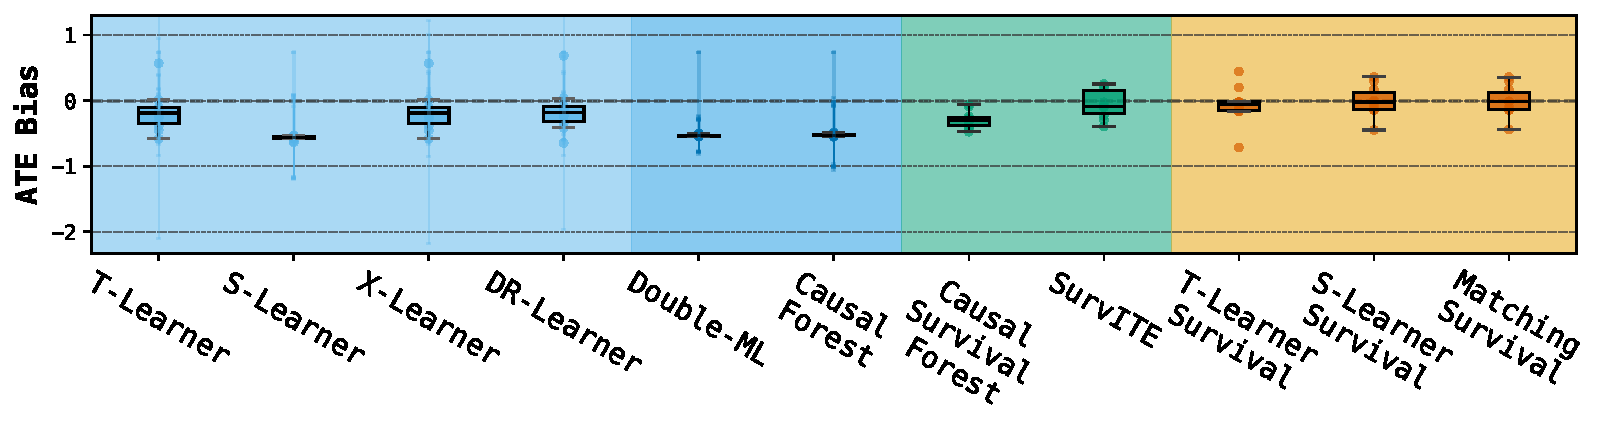
\includegraphics[width=\linewidth]{Appendices/appendix-ch04/images/figure_results_updated/ate_bias/Scenario_E_OBS-UConf_ate_bias.pdf}
        
    \end{minipage}}

    

    \subfloat[{RCT: \ChFourBlackCross, Ignorability: \ChFourGrayCheck, Positivity: \ChFourBlackCross, Ignorable Censoring: \ChFourGrayCheck}]{\begin{minipage}[t]{0.49\textwidth}
        \centering
        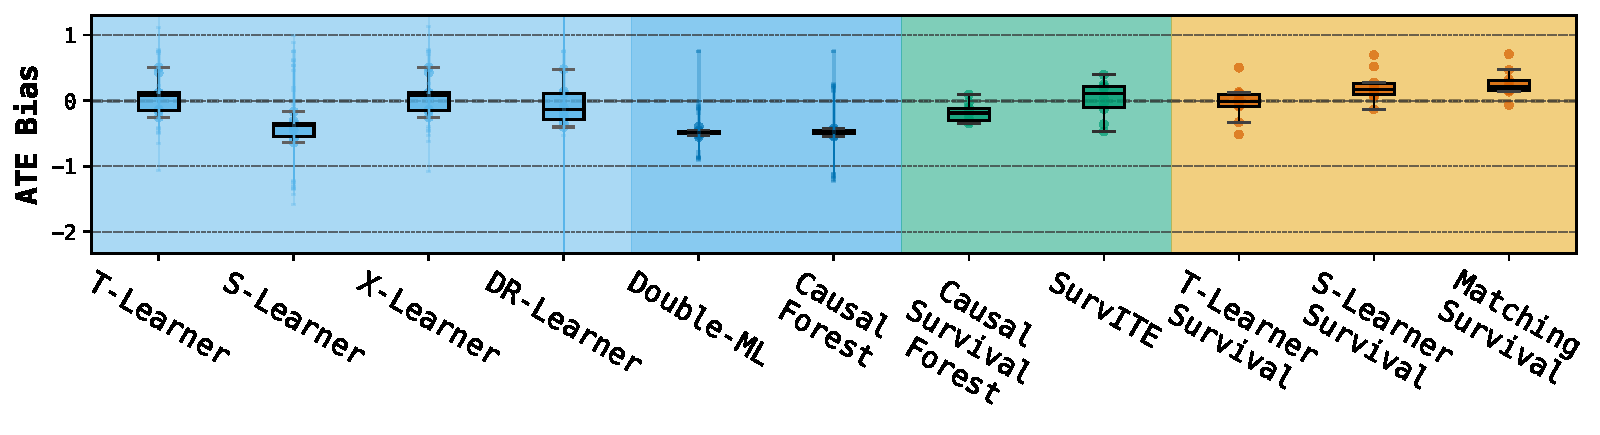
\includegraphics[width=\linewidth]{Appendices/appendix-ch04/images/figure_results_updated/ate_bias/Scenario_E_OBS-NoPos_ate_bias.pdf}
        
    \end{minipage}}
    \hfill
    \subfloat[{RCT: \ChFourBlackCross, Ignorability: \ChFourGrayCheck, Positivity: \ChFourGrayCheck, Ignorable Censoring: \ChFourBlackCross}]{\begin{minipage}[t]{0.49\textwidth}
        \centering
        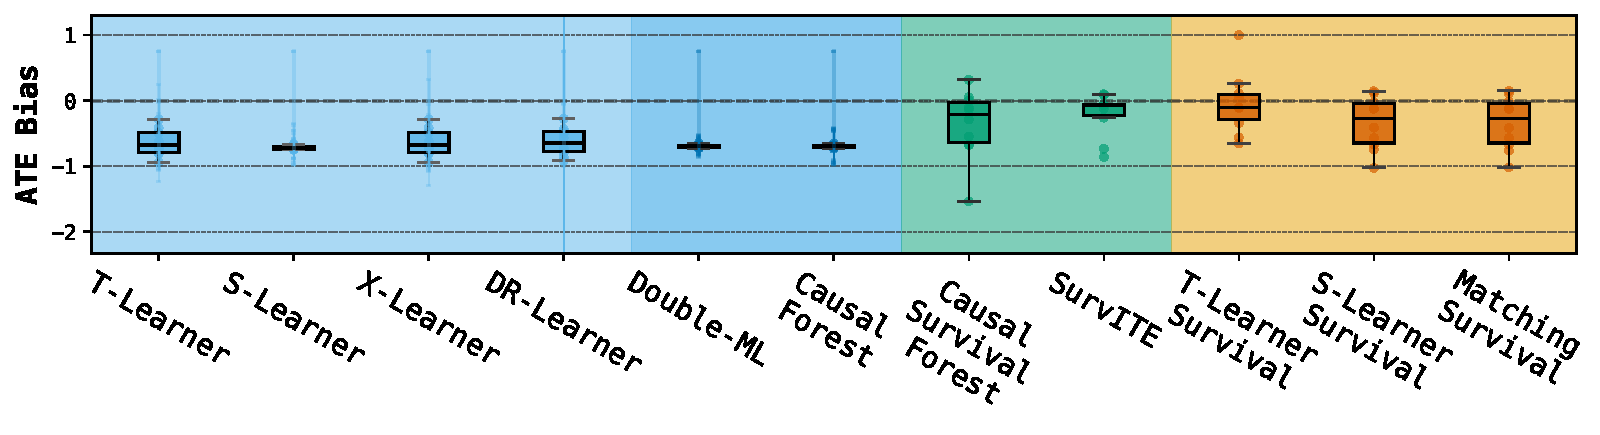
\includegraphics[width=\linewidth]{Appendices/appendix-ch04/images/figure_results_updated/ate_bias/Scenario_E_OBS-CPS-IC_ate_bias.pdf}
        
    \end{minipage}}

    

    \subfloat[{RCT: \ChFourBlackCross, Ignorability: \ChFourBlackCross, Positivity: \ChFourGrayCheck, Ignorable Censoring: \ChFourBlackCross}]{\begin{minipage}[t]{0.49\textwidth}
        \centering
        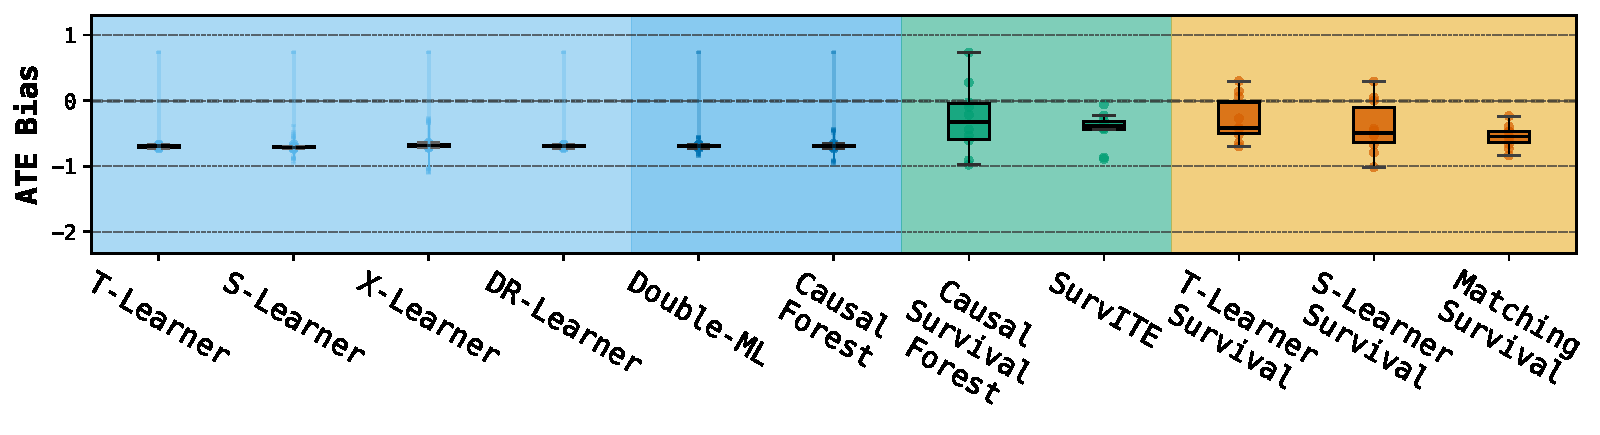
\includegraphics[width=\linewidth]{Appendices/appendix-ch04/images/figure_results_updated/ate_bias/Scenario_E_OBS-UConf-IC_ate_bias.pdf}
        
    \end{minipage}}
    \hfill
    \subfloat[{RCT: \ChFourBlackCross, Ignorability: \ChFourGrayCheck, Positivity: \ChFourBlackCross, Ignorable Censoring: \ChFourBlackCross}]{\begin{minipage}[t]{0.49\textwidth}
        \centering
        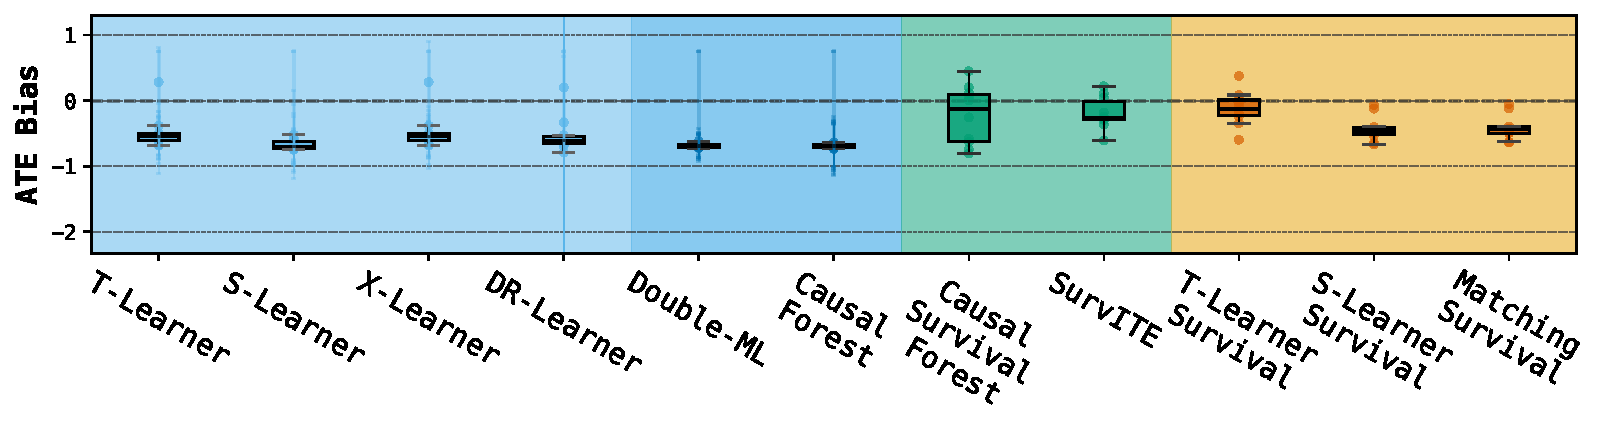
\includegraphics[width=\linewidth]{Appendices/appendix-ch04/images/figure_results_updated/ate_bias/Scenario_E_OBS-NoPos-IC_ate_bias.pdf}
        
    \end{minipage}}

                    \end{minipage}%
    }

    
    
}
\end{figure}






\subsubsection{Evaluation on auxiliary imputation and base learners}\label{ch04:app:auxiliary-eval-results}

In this section, we report the performance of auxiliary imputation and base regression or survival learners on the test sets.

\paragraph{Imputation evaluation}\label{ch04:subapp:impute-eval}

Table~\ref{ch04:tab:impute-eval} reports the MAE of the three imputation methods (Pseudo-obs, Margin, IPCW-T) across eight causal configurations and five censoring scenarios on the test sets.
Recall that Scenarios \texttt{A} and \texttt{B} have low censoring ($<$30\%), Scenario \texttt{C} medium (30--70\%), and Scenarios \texttt{D} and \texttt{E} high ($>$70\%), except it is switched in \texttt{-InfC} causal configurations, as mentioned in Appendix~\ref{ch04:app:synthetic-dataset}.
We can tell that the imputation method Pseudo-obs is only competitive under minimal censoring and suffers from high variability.
Margin imputation provides the best balance of accuracy and robustness, especially as censoring intensifies.
IPCW-T imputation improves over Pseudo-obs in most cases, but generally underperforms relative to Margin in medium‐ and high‐censor contexts.


% !TeX root = ../../../main.tex
\begin{table}[htbp]
\ChFourFloatContents{ch04:tab:impute-eval}{\caption{Evaluation on imputation methods across different survival scenarios and causal configurations. MAE between the imputed and true event times on testing set is reported as mean $\pm$ std. over 10 experimental repeats. ``Total Win'' row counts the number of survival configurations $\times$ random split combinations (8 × 10 = 80) in which each method achieved the lowest MAE, and is calculated within each scenario. The same rule applies to all the tables below in Appendix~\ref{ch04:app:auxiliary-eval-results}.}}{
    \centering
    
    
    \begin{adjustbox}{max width = 0.6\textwidth}
    \begin{tabular}{clccc}
    \toprule
        \multirow{2}{*}{\makecell[l]{\textbf{Survival}\\\textbf{Scenario}}} & \multirow{2}{*}{\makecell[l]{\textbf{Causal}\\\textbf{Configuration}}} & \multicolumn{3}{c}{\textbf{Imputation Method}}                   \\
    \cmidrule(r){3-5}
         &  & \textbf{Pseudo-obs} & \textbf{Margin} & \textbf{IPCW-T} \\ 
    \midrule
        \multirow{9}{*}{\texttt{A}}  & \texttt{RCT-50} & \ChFourBfTab{0.437$\pm$0.021} & 0.446$\pm$0.025 & 0.470$\pm$0.027 \\ 
        ~ & \texttt{RCT-5} & \ChFourBfTab{0.378$\pm$0.027} & 0.387$\pm$0.029 & 0.405$\pm$0.032 \\ 
        ~ & \texttt{OBS-CPS} & \ChFourBfTab{0.448$\pm$0.014} & 0.459$\pm$0.014 & 0.481$\pm$0.015 \\ 
        ~ & \texttt{OBS-UConf} & \ChFourBfTab{0.423$\pm$0.026} & 0.520$\pm$0.028 & 0.455$\pm$0.03 \\ 
        ~ & \texttt{OBS-NoPos} & \ChFourBfTab{0.411$\pm$0.023} & 0.420$\pm$0.023 & 0.442$\pm$0.025 \\ 
        ~ & \texttt{OBS-CPS-InfC} & 0.390$\pm$0.020 & \ChFourBfTab{0.374$\pm$0.014} & 0.388$\pm$0.014 \\ 
        ~ & \texttt{OBS-UConf-InfC} & 0.369$\pm$0.029 & 0.482$\pm$0.027 & \ChFourBfTab{0.362$\pm$0.028} \\ 
        ~ & \texttt{OBS-NoPos-InfC} & 0.347$\pm$0.023 & \ChFourBfTab{0.336$\pm$0.024} & 0.349$\pm$0.026 \\ 
    \cmidrule(r){2-5}
         & Total Win & 51 & 21 & 8 \\ 
    \midrule
        \multirow{9}{*}{\texttt{B}}  & \texttt{RCT-50} & 0.061$\pm$0.005 & 0.05$\pm$0.003 & \ChFourBfTab{0.048$\pm$0.004} \\ 
        ~ & \texttt{RCT-5} & 0.027$\pm$0.003 & 0.022$\pm$0.002 & \ChFourBfTab{0.021$\pm$0.003} \\ 
        ~ & \texttt{OBS-CPS} & 0.052$\pm$0.005 & 0.042$\pm$0.004 & \ChFourBfTab{0.040$\pm$0.003} \\ 
        ~ & \texttt{OBS-UConf} & 0.058$\pm$0.004 & 0.152$\pm$0.007 & \ChFourBfTab{0.046$\pm$0.004} \\ 
        ~ & \texttt{OBS-NoPos} & 0.068$\pm$0.008 & 0.057$\pm$0.005 & \ChFourBfTab{0.056$\pm$0.005} \\ 
        ~ & \texttt{OBS-CPS-InfC} & 0.039$\pm$0.005 & 0.037$\pm$0.005 & \ChFourBfTab{0.036$\pm$0.005} \\ 
        ~ & \texttt{OBS-UConf-InfC} & 0.040$\pm$0.004 & 0.140$\pm$0.005 & \ChFourBfTab{0.038$\pm$0.004} \\ 
        ~ & \texttt{OBS-NoPos-InfC} & 0.048$\pm$0.007 & 0.046$\pm$0.008 & \ChFourBfTab{0.045$\pm$0.008} \\ 
    \cmidrule(r){2-5}
         & Total Win & 0 & 3 & 77 \\ 
    \midrule
        \multirow{9}{*}{\texttt{C}}  & \texttt{RCT-50} & \ChFourBfTab{0.837$\pm$0.008} & 0.838$\pm$0.008 & 0.841$\pm$0.007 \\ 
        ~ & \texttt{RCT-5} & 0.803$\pm$0.013 & 0.804$\pm$0.013 & \ChFourBfTab{0.793$\pm$0.009} \\ 
        ~ & \texttt{OBS-CPS} & 0.829$\pm$0.014 & 0.830$\pm$0.014 & \ChFourBfTab{0.828$\pm$0.014} \\ 
        ~ & \texttt{OBS-UConf} & \ChFourBfTab{0.835$\pm$0.026} & 2.701$\pm$0.033 & 0.837$\pm$0.027 \\ 
        ~ & \texttt{OBS-NoPos} & \ChFourBfTab{0.845$\pm$0.014} & \ChFourBfTab{0.845$\pm$0.015} & 0.855$\pm$0.012 \\ 
        ~ & \texttt{OBS-CPS-InfC} & 2.786$\pm$0.079 & \ChFourBfTab{2.090$\pm$0.046} & 2.858$\pm$0.055 \\ 
        ~ & \texttt{OBS-UConf-InfC} & \ChFourBfTab{2.753$\pm$0.074} & 2.443$\pm$0.023 & 2.852$\pm$0.058 \\ 
        ~ & \texttt{OBS-NoPos-InfC} & 2.904$\pm$0.061 & \ChFourBfTab{2.197$\pm$0.045} & 3.006$\pm$0.034 \\ 
    \cmidrule(r){2-5}
         & Total Win & 23 & 35 & 22 \\ 
    \midrule
        \multirow{9}{*}{\texttt{D}}  & \texttt{RCT-50} & 3.303$\pm$0.333 & \ChFourBfTab{2.241$\pm$0.065} & 2.624$\pm$0.054 \\ 
        ~ & \texttt{RCT-5} & 2.897$\pm$0.257 & \ChFourBfTab{1.845$\pm$0.059} & 2.192$\pm$0.059 \\ 
        ~ & \texttt{OBS-CPS} & 3.191$\pm$0.449 & \ChFourBfTab{2.109$\pm$0.062} & 2.421$\pm$0.068 \\ 
        ~ & \texttt{OBS-UConf} & 3.463$\pm$0.706 & \ChFourBfTab{2.361$\pm$0.198} & 2.610$\pm$0.073 \\ 
        ~ & \texttt{OBS-NoPos} & 3.536$\pm$0.435 & \ChFourBfTab{2.404$\pm$0.074} & 2.853$\pm$0.072 \\ 
        ~ & \texttt{OBS-CPS-InfC} & 1.395$\pm$0.067 & \ChFourBfTab{1.289$\pm$0.064} & 1.366$\pm$0.068 \\ 
        ~ & \texttt{OBS-UConf-InfC} & 1.524$\pm$0.069 & 1.737$\pm$0.054 & \ChFourBfTab{1.511$\pm$0.063} \\ 
        ~ & \texttt{OBS-NoPos-InfC} & 1.689$\pm$0.074 & \ChFourBfTab{1.595$\pm$0.069} & 1.698$\pm$0.073 \\ 
    \cmidrule(r){2-5}
        & Total Win & 3 & 68 & 9 \\ 
    \midrule
        \multirow{9}{*}{\texttt{E}}  & \texttt{RCT-50} & 2.672$\pm$0.348 & \ChFourBfTab{1.595$\pm$0.019} & 2.033$\pm$0.022 \\ 
        ~ & \texttt{RCT-5} & 2.238$\pm$0.218 & \ChFourBfTab{1.468$\pm$0.023} & 1.823$\pm$0.023 \\ 
        ~ & \texttt{OBS-CPS} & 2.446$\pm$0.262 & \ChFourBfTab{1.577$\pm$0.022} & 1.992$\pm$0.032 \\ 
        ~ & \texttt{OBS-UConf} & 2.531$\pm$0.191 & 2.651$\pm$0.054 & \ChFourBfTab{2.051$\pm$0.031} \\ 
        ~ & \texttt{OBS-NoPos} & 2.669$\pm$0.288 & \ChFourBfTab{1.639$\pm$0.021} & 2.102$\pm$0.035 \\ 
        ~ & \texttt{OBS-CPS-InfC} & 3.324$\pm$0.136 & \ChFourBfTab{2.483$\pm$0.05} & 3.491$\pm$0.054 \\ 
        ~ & \texttt{OBS-UConf-InfC} & 3.346$\pm$0.147 & \ChFourBfTab{2.686$\pm$0.071} & 3.526$\pm$0.036 \\ 
        ~ & \texttt{OBS-NoPos-InfC} & 3.373$\pm$0.101 & \ChFourBfTab{2.541$\pm$0.038} & 3.648$\pm$0.072 \\  
    \cmidrule(r){2-5}
         & Total Win & 0 & 70 & 10 \\ 
    \bottomrule
    \end{tabular}
    \end{adjustbox}
}
\end{table}



\paragraph{Base regression learner evaluation} \label{ch04:subapp:base-reg-eval}
See Table~\ref{ch04:tab:base-s-learner}, \ref{ch04:tab:base-t-learner}, \ref{ch04:tab:base-x-learner}, \ref{ch04:tab:base-dr-learner} for MAE of prediction by the base regression learners for S-, T-, X-, DR-Learners.
The MAE is calculated by comparing a base learner's predicted event times and imputed event times by the imputation method (the latter is used as the ``ground truth'' for the base regression learners).
Since there are three imputation methods used, we first take the average of MAE across three different imputation methods within each random split, then report the mean and standard deviation of the average MAE across 10 experimental repeats with different random splits. 

See Table~\ref{ch04:tab:base-dr-learner-propensity} for the AUC on the evaluation of the predicted propensity score of DR-Learners.


% !TeX root = ../../../main.tex
\begin{table}[htbp]
\ChFourFloatContents{ch04:tab:base-s-learner}{\caption{S-Learner MAE}}{
    \centering
     
    \begin{adjustbox}{max width = 0.6\textwidth}
    \begin{tabular}{clccc}
    \toprule
        \multirow{2}{*}{\makecell[l]{\textbf{Survival}\\\textbf{Scenario}}} & \multirow{2}{*}{\makecell[l]{\textbf{Causal}\\\textbf{Configuration}}} & \multicolumn{3}{c}{\textbf{Base Regression Model}} \\ 
        \cmidrule(r){3-5}
         & & \textbf{Lasso Reg.} & \textbf{Random Forest} & \textbf{XGBoost} \\
    \midrule
        \multirow{9}{*}{\texttt{A}}   & \texttt{RCT-50} & 0.661$\pm$0.012 & \ChFourBfTab{0.655$\pm$0.014} & 0.671$\pm$0.013 \\ 
        ~ & \texttt{RCT-5} & \ChFourBfTab{0.645$\pm$0.011} & 0.649$\pm$0.012 & 0.667$\pm$0.014 \\ 
        ~ & \texttt{OBS-CPS} & 0.653$\pm$0.011 & \ChFourBfTab{0.646$\pm$0.010} & 0.662$\pm$0.012 \\ 
        ~ & \texttt{OBS-UConf} & \ChFourBfTab{0.604$\pm$0.009} & 0.608$\pm$0.009 & 0.620$\pm$0.007 \\ 
        ~ & \texttt{OBS-NoPos} & 0.657$\pm$0.010 & \ChFourBfTab{0.654$\pm$0.011} & 0.671$\pm$0.013 \\ 
        ~ & \texttt{OBS-CPS-InfC} & \ChFourBfTab{0.727$\pm$0.018} & 0.730$\pm$0.021 & 0.752$\pm$0.023 \\ 
        ~ & \texttt{OBS-UConf-InfC} & \ChFourBfTab{0.675$\pm$0.019} & 0.693$\pm$0.023 & 0.713$\pm$0.023 \\ 
        ~ & \texttt{OBS-NoPos-InfC} & \ChFourBfTab{0.724$\pm$0.014} & 0.732$\pm$0.018 & 0.755$\pm$0.02 \\ 
        \cmidrule(r){2-5}
        ~ & Total Win & 44 & 36 & 0 \\ 
    \midrule
        \multirow{9}{*}{\texttt{B}} & \texttt{RCT-50} & 0.33$\pm$0.008 & \ChFourBfTab{0.315$\pm$0.011} & 0.334$\pm$0.015 \\ 
        ~ & \texttt{RCT-5} & 0.278$\pm$0.006 & \ChFourBfTab{0.277$\pm$0.006} & 0.292$\pm$0.008 \\ 
        ~ & \texttt{OBS-CPS} & 0.315$\pm$0.011 & \ChFourBfTab{0.307$\pm$0.012} & 0.324$\pm$0.019 \\ 
        ~ & \texttt{OBS-UConf} & 0.354$\pm$0.007 & \ChFourBfTab{0.341$\pm$0.008} & 0.359$\pm$0.011 \\ 
        ~ & \texttt{OBS-NoPos} & 0.345$\pm$0.009 & \ChFourBfTab{0.323$\pm$0.011} & 0.341$\pm$0.011 \\ 
        ~ & \texttt{OBS-CPS-InfC} & 0.301$\pm$0.007 & \ChFourBfTab{0.294$\pm$0.006} & 0.309$\pm$0.008 \\ 
        ~ & \texttt{OBS-UConf-InfC} & 0.34$\pm$0.004 & \ChFourBfTab{0.328$\pm$0.005} & 0.347$\pm$0.006 \\ 
        ~ & \texttt{OBS-NoPos-InfC} & 0.337$\pm$0.005 & \ChFourBfTab{0.319$\pm$0.006} & 0.337$\pm$0.007 \\ 
        \cmidrule(r){2-5}
        ~ & Total Win & 3 & 77 & 0 \\ 
    \midrule
        \multirow{9}{*}{\texttt{C}} & \texttt{RCT-50} & \ChFourBfTab{1.430$\pm$0.022} & 1.593$\pm$0.025 & 1.738$\pm$0.024 \\ 
        ~ & \texttt{RCT-5} & \ChFourBfTab{1.403$\pm$0.019} & 1.532$\pm$0.018 & 1.687$\pm$0.027 \\ 
        ~ & \texttt{OBS-CPS} & \ChFourBfTab{1.409$\pm$0.021} & 1.555$\pm$0.025 & 1.706$\pm$0.028 \\ 
        ~ & \texttt{OBS-UConf} & \ChFourBfTab{1.419$\pm$0.023} & 1.563$\pm$0.026 & 1.721$\pm$0.020 \\ 
        ~ & \texttt{OBS-NoPos} & \ChFourBfTab{1.453$\pm$0.019} & 1.612$\pm$0.024 & 1.755$\pm$0.022 \\ 
        ~ & \texttt{OBS-CPS-InfC} & \ChFourBfTab{0.931$\pm$0.027} & 1.011$\pm$0.03 & 1.148$\pm$0.045 \\ 
        ~ & \texttt{OBS-UConf-InfC} & \ChFourBfTab{0.895$\pm$0.033} & 0.966$\pm$0.04 & 1.096$\pm$0.059 \\ 
        ~ & \texttt{OBS-NoPos-InfC} & \ChFourBfTab{0.916$\pm$0.057} & 1.003$\pm$0.067 & 1.123$\pm$0.086 \\ 
        \cmidrule(r){2-5}
        ~ & Total Win & 80 & 0 & 0 \\ 
    \midrule
        \multirow{9}{*}{\texttt{D}} & \texttt{RCT-50} & \ChFourBfTab{0.941$\pm$0.18} & 1.002$\pm$0.202 & 1.082$\pm$0.206 \\ 
        ~ & \texttt{RCT-5} & \ChFourBfTab{1.016$\pm$0.121} & 1.095$\pm$0.123 & 1.210$\pm$0.248 \\ 
        ~ & \texttt{OBS-CPS} & \ChFourBfTab{1.031$\pm$0.258} & 1.082$\pm$0.264 & 1.188$\pm$0.345 \\ 
        ~ & \texttt{OBS-UConf} & \ChFourBfTab{0.985$\pm$0.34} & 1.015$\pm$0.300 & 1.073$\pm$0.383 \\ 
        ~ & \texttt{OBS-NoPos} & \ChFourBfTab{0.967$\pm$0.238} & 1.03$\pm$0.249 & 1.107$\pm$0.295 \\ 
        ~ & \texttt{OBS-CPS-InfC} & \ChFourBfTab{1.146$\pm$0.030} & 1.148$\pm$0.034 & 1.209$\pm$0.044 \\ 
        ~ & \texttt{OBS-UConf-InfC} & 1.179$\pm$0.024 & \ChFourBfTab{1.172$\pm$0.031} & 1.234$\pm$0.032 \\ 
        ~ & \texttt{OBS-NoPos-InfC} & \ChFourBfTab{1.169$\pm$0.026} & \ChFourBfTab{1.169$\pm$0.026} & 1.230$\pm$0.028 \\ 
        \cmidrule(r){2-5}
        ~ & Total Win & 48 & 29 & 3 \\ 
    \midrule
        \multirow{9}{*}{\texttt{E}} & \texttt{RCT-50} & \ChFourBfTab{1.75$\pm$0.186} & 1.906$\pm$0.207 & 2.124$\pm$0.247 \\ 
        ~ & \texttt{RCT-5} & \ChFourBfTab{1.604$\pm$0.125} & 1.731$\pm$0.133 & 1.901$\pm$0.17 \\ 
        ~ & \texttt{OBS-CPS} & \ChFourBfTab{1.651$\pm$0.161} & 1.799$\pm$0.201 & 1.990$\pm$0.243 \\ 
        ~ & \texttt{OBS-UConf} & \ChFourBfTab{1.630$\pm$0.127} & 1.779$\pm$0.159 & 1.974$\pm$0.212 \\ 
        ~ & \texttt{OBS-NoPos} & \ChFourBfTab{1.698$\pm$0.139} & 1.856$\pm$0.162 & 2.059$\pm$0.202 \\ 
        ~ & \texttt{OBS-CPS-InfC} & \ChFourBfTab{0.917$\pm$0.089} & 1.012$\pm$0.113 & 1.140$\pm$0.141 \\ 
        ~ & \texttt{OBS-UConf-InfC} & \ChFourBfTab{0.968$\pm$0.130} & 1.074$\pm$0.164 & 1.222$\pm$0.237 \\ 
        ~ & \texttt{OBS-NoPos-InfC} & \ChFourBfTab{0.928$\pm$0.060} & 1.012$\pm$0.063 & 1.130$\pm$0.071 \\ 
        \cmidrule(r){2-5}
        ~ & Total Win & 80 & 0 & 0 \\ 
    \bottomrule
    \end{tabular}
    \end{adjustbox}
}
\end{table}




% !TeX root = ../../../main.tex
\begin{table}[htbp]
\ChFourFloatContents{ch04:tab:base-t-learner}{\caption{T-Learner MAE}}{
    \centering
     
    \begin{adjustbox}{max width=1\textwidth}
    \begin{tabular}{clccc|ccc}
    \toprule
        \multirow{2}{*}{\makecell[l]{\textbf{Survival}\\\textbf{Scenario}}} & \multirow{2}{*}{\makecell[l]{\textbf{Causal}\\\textbf{Configuration}}} & \multicolumn{3}{c}{\textbf{Base Regression Model (Treated)}} & \multicolumn{3}{c}{\textbf{Base Regression Model (Control)}} \\ 
        \cmidrule(r){3-5} \cmidrule(r){6-8}
        & & \textbf{Lasso Reg.} & \textbf{Random Forest} & \textbf{XGBoost} & \textbf{Lasso Reg.} & \textbf{Random Forest} & \textbf{XGBoost} \\
        \midrule
        \multirow{9}{*}{\texttt{A}} & \texttt{RCT-50} & 0.669$\pm$0.012 & \ChFourBfTab{0.652$\pm$0.013} & 0.680$\pm$0.015 & \ChFourBfTab{0.652$\pm$0.019} & 0.657$\pm$0.019 & 0.685$\pm$0.019 \\ 
        ~ &\texttt{RCT-5} & 0.656$\pm$0.044 & \ChFourBfTab{0.641$\pm$0.049} & 0.677$\pm$0.050 & \ChFourBfTab{0.644$\pm$0.011} & 0.650$\pm$0.012 & 0.668$\pm$0.014 \\ 
        ~ &\texttt{OBS-CPS} & 0.711$\pm$0.012 & \ChFourBfTab{0.697$\pm$0.012} & 0.727$\pm$0.012 & \ChFourBfTab{0.588$\pm$0.014} & 0.595$\pm$0.014 & 0.621$\pm$0.018 \\ 
        ~ &\texttt{OBS-UConf} & \ChFourBfTab{0.640$\pm$0.009} & 0.641$\pm$0.007 & 0.668$\pm$0.005 & \ChFourBfTab{0.558$\pm$0.012} & 0.566$\pm$0.013 & 0.593$\pm$0.015 \\ 
        ~ &\texttt{OBS-NoPos} & 0.568$\pm$0.014 & \ChFourBfTab{0.561$\pm$0.013} & 0.587$\pm$0.016 & \ChFourBfTab{0.733$\pm$0.015} & 0.747$\pm$0.016 & 0.776$\pm$0.016 \\ 
        ~ &\texttt{OBS-CPS-InfC} & 0.799$\pm$0.020 & \ChFourBfTab{0.797$\pm$0.022} & 0.838$\pm$0.023 & \ChFourBfTab{0.646$\pm$0.023} & 0.664$\pm$0.025 & 0.699$\pm$0.029 \\ 
        ~ &\texttt{OBS-UConf-InfC} & \ChFourBfTab{0.723$\pm$0.023} & 0.740$\pm$0.031 & 0.778$\pm$0.030 & \ChFourBfTab{0.614$\pm$0.019} & 0.633$\pm$0.023 & 0.668$\pm$0.025 \\ 
        ~ &\texttt{OBS-NoPos-InfC} & \ChFourBfTab{0.608$\pm$0.018} & 0.609$\pm$0.016 & 0.642$\pm$0.020 & \ChFourBfTab{0.824$\pm$0.021} & 0.855$\pm$0.021 & 0.895$\pm$0.029 \\ 
        \cmidrule(r){2-5} \cmidrule(r){6-8}
        ~ &Total Win & 28 & 52 & 0 & 77 & 3 & 0 \\ 
        \midrule
        \multirow{9}{*}{\texttt{B}} & \texttt{RCT-50} & 0.375$\pm$0.012 & \ChFourBfTab{0.350$\pm$0.014} & 0.374$\pm$0.016 & \ChFourBfTab{0.279$\pm$0.007} & 0.281$\pm$0.008 & 0.303$\pm$0.006 \\ 
        ~ & \texttt{RCT-5} & 0.393$\pm$0.051 & \ChFourBfTab{0.383$\pm$0.047} & 0.404$\pm$0.043 & \ChFourBfTab{0.271$\pm$0.005} & 0.273$\pm$0.005 & 0.287$\pm$0.006 \\ 
        ~ & \texttt{OBS-CPS} & 0.326$\pm$0.014 & \ChFourBfTab{0.302$\pm$0.014} & 0.322$\pm$0.016 & \ChFourBfTab{0.305$\pm$0.011} & 0.313$\pm$0.012 & 0.338$\pm$0.015 \\ 
        ~ & \texttt{OBS-UConf} & 0.375$\pm$0.008 & \ChFourBfTab{0.348$\pm$0.009} & 0.371$\pm$0.011 & \ChFourBfTab{0.327$\pm$0.008} & 0.334$\pm$0.007 & 0.363$\pm$0.012 \\ 
        ~ & \texttt{OBS-NoPos} & 0.425$\pm$0.014 & \ChFourBfTab{0.411$\pm$0.015} & 0.442$\pm$0.017 & \ChFourBfTab{0.231$\pm$0.007} & 0.235$\pm$0.007 & 0.253$\pm$0.008 \\ 
        ~ & \texttt{OBS-CPS-InfC} & 0.311$\pm$0.007 & \ChFourBfTab{0.292$\pm$0.006} & 0.311$\pm$0.008 & \ChFourBfTab{0.291$\pm$0.009} & 0.297$\pm$0.010 & 0.322$\pm$0.011 \\ 
        ~ & \texttt{OBS-UConf-InfC} & 0.365$\pm$0.004 & \ChFourBfTab{0.344$\pm$0.007} & 0.370$\pm$0.009 & \ChFourBfTab{0.310$\pm$0.007} & 0.313$\pm$0.007 & 0.337$\pm$0.008 \\ 
        ~ & \texttt{OBS-NoPos-InfC} & 0.415$\pm$0.009 & \ChFourBfTab{0.406$\pm$0.009} & 0.438$\pm$0.011 & \ChFourBfTab{0.228$\pm$0.005} & 0.233$\pm$0.006 & 0.249$\pm$0.006 \\ 
        \cmidrule(r){2-5} \cmidrule(r){6-8}
        ~ & Total Win & 4 & 76 & 0 & 68 & 12 & 0 \\ 
        \midrule
        \multirow{9}{*}{\texttt{C}} & \texttt{RCT-50} & \ChFourBfTab{1.534$\pm$0.037} & 1.653$\pm$0.041 & 1.839$\pm$0.046 & \ChFourBfTab{1.387$\pm$0.029} & 1.542$\pm$0.020 & 1.747$\pm$0.027 \\ 
        ~ & \texttt{RCT-5} & \ChFourBfTab{1.643$\pm$0.091} & 1.751$\pm$0.085 & 1.935$\pm$0.074 & \ChFourBfTab{1.393$\pm$0.020} & 1.527$\pm$0.02 & 1.688$\pm$0.021 \\ 
        ~ & \texttt{OBS-CPS} & \ChFourBfTab{1.484$\pm$0.026} & 1.599$\pm$0.031 & 1.797$\pm$0.036 & \ChFourBfTab{1.379$\pm$0.030} & 1.529$\pm$0.029 & 1.726$\pm$0.033 \\ 
        ~ & \texttt{OBS-UConf} & \ChFourBfTab{1.493$\pm$0.037} & 1.617$\pm$0.034 & 1.809$\pm$0.028 & \ChFourBfTab{1.363$\pm$0.019} & 1.528$\pm$0.021 & 1.740$\pm$0.027 \\ 
        ~ & \texttt{OBS-NoPos} & \ChFourBfTab{1.568$\pm$0.040} & 1.665$\pm$0.038 & 1.860$\pm$0.037 & \ChFourBfTab{1.420$\pm$0.037} & 1.565$\pm$0.027 & 1.763$\pm$0.035 \\ 
        ~ & \texttt{OBS-CPS-InfC} & \ChFourBfTab{0.909$\pm$0.047} & 1.002$\pm$0.052 & 1.144$\pm$0.050 & \ChFourBfTab{0.953$\pm$0.042} & 1.040$\pm$0.048 & 1.198$\pm$0.060 \\ 
        ~ & \texttt{OBS-UConf-InfC} & \ChFourBfTab{0.876$\pm$0.039} & 0.951$\pm$0.052 & 1.088$\pm$0.070 & \ChFourBfTab{0.916$\pm$0.044} & 1.004$\pm$0.056 & 1.166$\pm$0.079 \\ 
        ~ & \texttt{OBS-NoPos-InfC} & \ChFourBfTab{0.902$\pm$0.057} & 1.009$\pm$0.074 & 1.149$\pm$0.088 & \ChFourBfTab{0.928$\pm$0.076} & 1.016$\pm$0.087 & 1.152$\pm$0.088 \\ 
        \cmidrule(r){2-5} \cmidrule(r){6-8}
        ~ & Total Win & 79 & 1 & 0 & 80 & 0 & 0 \\ 
        \midrule
        \multirow{9}{*}{\texttt{D}} & \texttt{RCT-50} & \ChFourBfTab{0.302$\pm$0.083} & 0.316$\pm$0.093 & 0.339$\pm$0.11 & \ChFourBfTab{1.546$\pm$0.304} & 1.691$\pm$0.484 & 1.767$\pm$0.429 \\ 
        ~ & \texttt{RCT-5} & \ChFourBfTab{0.284$\pm$0.044} & 0.296$\pm$0.049 & 0.312$\pm$0.052 & \ChFourBfTab{1.051$\pm$0.127} & 1.118$\pm$0.129 & 1.285$\pm$0.304 \\ 
        ~ & \texttt{OBS-CPS} & \ChFourBfTab{0.347$\pm$0.084} & 0.366$\pm$0.087 & 0.384$\pm$0.094 & \ChFourBfTab{1.651$\pm$0.416} & 1.758$\pm$0.443 & 1.924$\pm$0.594 \\ 
        ~ & \texttt{OBS-UConf} & \ChFourBfTab{0.328$\pm$0.134} & 0.343$\pm$0.130 & 0.362$\pm$0.138 & \ChFourBfTab{1.691$\pm$0.564} & 1.797$\pm$0.529 & 1.809$\pm$0.705 \\ 
        ~ & \texttt{OBS-NoPos} & \ChFourBfTab{0.334$\pm$0.105} & 0.342$\pm$0.117 & 0.366$\pm$0.129 & \ChFourBfTab{1.571$\pm$0.382} & 1.659$\pm$0.392 & 1.939$\pm$0.612 \\ 
        ~ & \texttt{OBS-CPS-InfC} & 1.138$\pm$0.029 & \ChFourBfTab{1.097$\pm$0.027} & 1.171$\pm$0.028 & \ChFourBfTab{1.147$\pm$0.041} & 1.201$\pm$0.051 & 1.300$\pm$0.056 \\ 
        ~ & \texttt{OBS-UConf-InfC} & 1.206$\pm$0.029 & \ChFourBfTab{1.156$\pm$0.043} & 1.240$\pm$0.044 & \ChFourBfTab{1.146$\pm$0.023} & 1.197$\pm$0.028 & 1.298$\pm$0.029 \\ 
        ~ & \texttt{OBS-NoPos-InfC} & 1.216$\pm$0.030 & \ChFourBfTab{1.198$\pm$0.035} & 1.297$\pm$0.046 & \ChFourBfTab{1.100$\pm$0.030} & 1.143$\pm$0.037 & 1.222$\pm$0.035 \\ 
        \cmidrule(r){2-5} \cmidrule(r){6-8}
        ~ & Total Win & 45 & 35 & 0 & 66 & 10 & 4 \\ 
        \midrule
        \multirow{9}{*}{\texttt{E}}  & \texttt{RCT-50} & \ChFourBfTab{1.784$\pm$0.230} & 1.955$\pm$0.255 & 2.22$\pm$0.310 & \ChFourBfTab{1.720$\pm$0.154} & 1.899$\pm$0.184 & 2.108$\pm$0.198 \\ 
        ~ & \texttt{RCT-5} & \ChFourBfTab{1.607$\pm$0.244} & 1.859$\pm$0.436 & 1.969$\pm$0.335 & \ChFourBfTab{1.605$\pm$0.121} & 1.733$\pm$0.131 & 1.894$\pm$0.147 \\ 
        ~ & \texttt{OBS-CPS} & \ChFourBfTab{1.670$\pm$0.194} & 1.852$\pm$0.261 & 2.092$\pm$0.312 & \ChFourBfTab{1.637$\pm$0.141} & 1.785$\pm$0.158 & 1.993$\pm$0.200 \\ 
        ~ & \texttt{OBS-UConf} & \ChFourBfTab{1.650$\pm$0.145} & 1.809$\pm$0.167 & 2.053$\pm$0.239 & \ChFourBfTab{1.616$\pm$0.130} & 1.763$\pm$0.144 & 1.982$\pm$0.201 \\ 
        ~ & \texttt{OBS-NoPos} & \ChFourBfTab{1.740$\pm$0.161} & 1.907$\pm$0.200 & 2.198$\pm$0.338 & \ChFourBfTab{1.663$\pm$0.140} & 1.804$\pm$0.148 & 2.027$\pm$0.167 \\ 
        ~ & \texttt{OBS-CPS-InfC} & \ChFourBfTab{0.911$\pm$0.111} & 1.007$\pm$0.123 & 1.146$\pm$0.140 & \ChFourBfTab{0.925$\pm$0.074} & 1.015$\pm$0.096 & 1.158$\pm$0.104 \\ 
        ~ & \texttt{OBS-UConf-InfC} & \ChFourBfTab{0.953$\pm$0.107} & 1.049$\pm$0.118 & 1.221$\pm$0.146 & \ChFourBfTab{0.987$\pm$0.159} & 1.103$\pm$0.222 & 1.271$\pm$0.228 \\ 
        ~ & \texttt{OBS-NoPos-InfC} & \ChFourBfTab{0.949$\pm$0.085} & 1.043$\pm$0.095 & 1.221$\pm$0.112 & \ChFourBfTab{0.908$\pm$0.046} & 1.000$\pm$0.044 & 1.136$\pm$0.064 \\ 
        \cmidrule(r){2-5} \cmidrule(r){6-8}
        ~ & Total Win & 80 & 0 & 0 & 80 & 0 & 0 \\ 
    \bottomrule
    \end{tabular}
    \end{adjustbox}
}
\end{table}



% !TeX root = ../../../main.tex
\begin{table}[htbp]
\ChFourFloatContents{ch04:tab:base-x-learner}{\caption{X-Learner MAE}}{
    \centering
     
    \begin{adjustbox}{max width=1\textwidth}
    \begin{tabular}{clccc|ccc}
    \toprule
        \multirow{2}{*}{\makecell[l]{\textbf{Survival}\\\textbf{Scenario}}} & \multirow{2}{*}{\makecell[l]{\textbf{Causal}\\\textbf{Configuration}}} & \multicolumn{3}{c}{\textbf{Base Regression Model (Treated)}} & \multicolumn{3}{c}{\textbf{Base Regression Model (Control)}} \\ 
        \cmidrule(r){3-5} \cmidrule(r){6-8}
        & & \textbf{Lasso Reg.} & \textbf{Random Forest} & \textbf{XGBoost} & \textbf{Lasso Reg.} & \textbf{Random Forest} & \textbf{XGBoost} \\
        \midrule
        \multirow{9}{*}{\texttt{A}} & \texttt{RCT-50} & \ChFourBfTab 0.620$\pm$0.011 & 0.622$\pm$0.013 & 0.631$\pm$0.013 & \ChFourBfTab 0.624$\pm$0.019 & \ChFourBfTab 0.624$\pm$0.019 & 0.631$\pm$0.018 \\
        ~ & \texttt{RCT-5} & \ChFourBfTab 0.613$\pm$0.048 & 0.624$\pm$0.056 & 0.634$\pm$0.050 & 0.618$\pm$0.012 & \ChFourBfTab 0.617$\pm$0.012 & 0.623$\pm$0.010 \\
        ~ & \texttt{OBS-CPS} & \ChFourBfTab 0.664$\pm$0.011 & 0.667$\pm$0.010 & 0.675$\pm$0.012 & \ChFourBfTab 0.561$\pm$0.013 & 0.562$\pm$0.014 & 0.568$\pm$0.013 \\
        ~ & \texttt{OBS-UConf} & \ChFourBfTab 0.608$\pm$0.008 & 0.610$\pm$0.008 & 0.616$\pm$0.008 & \ChFourBfTab 0.530$\pm$0.012 & 0.531$\pm$0.012 & 0.538$\pm$0.012 \\
        ~ & \texttt{OBS-NoPos} & \ChFourBfTab 0.532$\pm$0.013 & 0.533$\pm$0.013 & 0.539$\pm$0.015 & \ChFourBfTab 0.711$\pm$0.014 & 0.712$\pm$0.014 & 0.718$\pm$0.015 \\
        ~ & \texttt{OBS-CPS-InfC} & \ChFourBfTab 0.747$\pm$0.018 & 0.751$\pm$0.018 & 0.763$\pm$0.019 & \ChFourBfTab 0.616$\pm$0.021 & \ChFourBfTab 0.616$\pm$0.022 & 0.623$\pm$0.022 \\
        ~ & \texttt{OBS-UConf-InfC} & \ChFourBfTab 0.689$\pm$0.024 & 0.691$\pm$0.023 & 0.698$\pm$0.024 & \ChFourBfTab 0.583$\pm$0.019 & 0.585$\pm$0.020 & 0.592$\pm$0.019 \\
        ~ & \texttt{OBS-NoPos-InfC} & \ChFourBfTab 0.570$\pm$0.016 & \ChFourBfTab 0.570$\pm$0.017 & 0.578$\pm$0.018 & \ChFourBfTab 0.800$\pm$0.021 & 0.802$\pm$0.021 & 0.809$\pm$0.020 \\
        \cmidrule(r){2-5} \cmidrule(r){6-8}
        ~ & Total Win & 64 & 16 & 0 & 47 & 33 & 0 \\
        \midrule
        \multirow{9}{*}{\texttt{B}} & \texttt{RCT-50} & 0.339$\pm$0.012 & \ChFourBfTab 0.328$\pm$0.012 & 0.333$\pm$0.012 & 0.265$\pm$0.007 & \ChFourBfTab 0.261$\pm$0.007 & 0.264$\pm$0.007 \\
        ~ & \texttt{RCT-5} & 0.365$\pm$0.045 & \ChFourBfTab 0.364$\pm$0.051 & 0.368$\pm$0.046 & 0.256$\pm$0.005 & \ChFourBfTab 0.253$\pm$0.004 & 0.255$\pm$0.004 \\
        ~ & \texttt{OBS-CPS} & 0.296$\pm$0.014 & \ChFourBfTab 0.283$\pm$0.013 & 0.287$\pm$0.013 & \ChFourBfTab 0.290$\pm$0.010 & \ChFourBfTab 0.290$\pm$0.012 & 0.291$\pm$0.011 \\
        ~ & \texttt{OBS-UConf} & 0.339$\pm$0.009 & \ChFourBfTab 0.327$\pm$0.008 & 0.331$\pm$0.008 & 0.312$\pm$0.008 & \ChFourBfTab 0.309$\pm$0.006 & 0.311$\pm$0.008 \\
        ~ & \texttt{OBS-NoPos} & 0.396$\pm$0.013 & \ChFourBfTab 0.387$\pm$0.014 & 0.393$\pm$0.013 & 0.221$\pm$0.006 & \ChFourBfTab 0.217$\pm$0.007 & 0.219$\pm$0.007 \\
        ~ & \texttt{OBS-CPS-InfC} & 0.283$\pm$0.006 & \ChFourBfTab 0.272$\pm$0.007 & 0.275$\pm$0.006 & 0.277$\pm$0.008 & \ChFourBfTab 0.275$\pm$0.008 & 0.278$\pm$0.009 \\
        ~ & \texttt{OBS-UConf-InfC} & 0.332$\pm$0.005 & \ChFourBfTab 0.321$\pm$0.006 & 0.326$\pm$0.006 & 0.295$\pm$0.008 & \ChFourBfTab 0.291$\pm$0.007 & 0.293$\pm$0.007 \\
        ~ & \texttt{OBS-NoPos-InfC} & 0.388$\pm$0.008 & \ChFourBfTab 0.379$\pm$0.008 & 0.386$\pm$0.008 & 0.219$\pm$0.005 & \ChFourBfTab 0.215$\pm$0.005 & 0.216$\pm$0.005 \\
        \cmidrule(r){2-5} \cmidrule(r){6-8}
        ~ & Total Win & 3 & 73 & 4 & 5 & 70 & 5 \\
        \midrule
        \multirow{9}{*}{\texttt{C}} & \texttt{RCT-50} & 1.542$\pm$0.041 & 1.547$\pm$0.032 & \ChFourBfTab 1.533$\pm$0.033 & 1.417$\pm$0.025 & 1.422$\pm$0.023 & \ChFourBfTab 1.403$\pm$0.026 \\
        ~ & \texttt{RCT-5} & 1.651$\pm$0.092 & 1.662$\pm$0.091 & \ChFourBfTab 1.640$\pm$0.087 & 1.411$\pm$0.018 & 1.414$\pm$0.019 & \ChFourBfTab 1.400$\pm$0.019 \\
        ~ & \texttt{OBS-CPS} & 1.492$\pm$0.031 & 1.492$\pm$0.031 & \ChFourBfTab 1.481$\pm$0.026 & 1.409$\pm$0.032 & 1.413$\pm$0.030 & \ChFourBfTab 1.394$\pm$0.031 \\
        ~ & \texttt{OBS-UConf} & 1.509$\pm$0.038 & 1.510$\pm$0.039 & \ChFourBfTab 1.497$\pm$0.042 & 1.396$\pm$0.016 & 1.402$\pm$0.014 & \ChFourBfTab 1.385$\pm$0.016 \\
        ~ & \texttt{OBS-NoPos} & 1.562$\pm$0.042 & 1.563$\pm$0.038 & \ChFourBfTab 1.561$\pm$0.038 & 1.445$\pm$0.033 & 1.449$\pm$0.035 & \ChFourBfTab 1.433$\pm$0.037 \\
        ~ & \texttt{OBS-CPS-InfC} & \ChFourBfTab 0.909$\pm$0.047 & 0.915$\pm$0.048 & \ChFourBfTab 0.909$\pm$0.046 & \ChFourBfTab 0.952$\pm$0.043 & 0.959$\pm$0.041 & 0.954$\pm$0.043 \\
        ~ & \texttt{OBS-UConf-InfC} & 0.876$\pm$0.039 & 0.879$\pm$0.042 & \ChFourBfTab 0.875$\pm$0.039 & \ChFourBfTab 0.916$\pm$0.044 & 0.921$\pm$0.045 & 0.919$\pm$0.047 \\
        ~ & \texttt{OBS-NoPos-InfC} & \ChFourBfTab 0.902$\pm$0.058 & 0.909$\pm$0.061 & 0.904$\pm$0.060 & \ChFourBfTab 0.928$\pm$0.076 & 0.935$\pm$0.081 & \ChFourBfTab 0.928$\pm$0.074 \\
        \cmidrule(r){2-5} \cmidrule(r){6-8}
        ~ & Total Win & 27 & 11 & 42 & 17 & 7 & 56 \\
        \midrule
        \multirow{9}{*}{\texttt{D}} & \texttt{RCT-50} & 0.306$\pm$0.088 & 0.300$\pm$0.089 & \ChFourBfTab 0.292$\pm$0.083 & 1.633$\pm$0.342 & 1.613$\pm$0.503 & \ChFourBfTab 1.506$\pm$0.302 \\
        ~ & \texttt{RCT-5} & 0.283$\pm$0.046 & 0.280$\pm$0.042 & \ChFourBfTab 0.277$\pm$0.047 & 1.124$\pm$0.125 & 1.055$\pm$0.128 & \ChFourBfTab 1.033$\pm$0.150 \\
        ~ & \texttt{OBS-CPS} & 0.355$\pm$0.085 & 0.343$\pm$0.080 & \ChFourBfTab 0.334$\pm$0.081 & 1.819$\pm$0.545 & 1.681$\pm$0.456 & \ChFourBfTab 1.613$\pm$0.436 \\
        ~ & \texttt{OBS-UConf} & 0.336$\pm$0.137 & 0.324$\pm$0.126 & \ChFourBfTab 0.322$\pm$0.123 & 1.772$\pm$0.571 & 1.737$\pm$0.498 & \ChFourBfTab 1.613$\pm$0.557 \\
        ~ & \texttt{OBS-NoPos} & 0.336$\pm$0.110 & 0.322$\pm$0.106 & \ChFourBfTab 0.319$\pm$0.104 & 1.688$\pm$0.418 & 1.607$\pm$0.383 & \ChFourBfTab 1.540$\pm$0.388 \\
        ~ & \texttt{OBS-CPS-InfC} & 1.067$\pm$0.026 & \ChFourBfTab 1.043$\pm$0.025 & 1.049$\pm$0.026 & \ChFourBfTab 1.133$\pm$0.041 & 1.137$\pm$0.043 & 1.136$\pm$0.043 \\
        ~ & \texttt{OBS-UConf-InfC} & 1.116$\pm$0.032 & \ChFourBfTab 1.098$\pm$0.033 & 1.103$\pm$0.027 & \ChFourBfTab 1.135$\pm$0.021 & 1.138$\pm$0.021 & 1.136$\pm$0.021 \\
        ~ & \texttt{OBS-NoPos-InfC} & 1.160$\pm$0.029 & \ChFourBfTab 1.137$\pm$0.029 & 1.140$\pm$0.029 & \ChFourBfTab 1.085$\pm$0.032 & 1.088$\pm$0.032 & 1.087$\pm$0.031 \\
        \cmidrule(r){2-5} \cmidrule(r){6-8}
        ~ & Total Win & 4 & 36 & 40 & 17 & 21 & 42 \\
        \midrule
        \multirow{9}{*}{\texttt{E}} & \texttt{RCT-50} & \ChFourBfTab 1.771$\pm$0.226 & 1.798$\pm$0.237 & 1.772$\pm$0.230 & 1.734$\pm$0.154 & 1.748$\pm$0.156 & \ChFourBfTab 1.721$\pm$0.150 \\
        ~ & \texttt{RCT-5} & \ChFourBfTab 1.607$\pm$0.240 & 1.731$\pm$0.366 & 1.608$\pm$0.245 & 1.602$\pm$0.120 & 1.606$\pm$0.121 & \ChFourBfTab 1.597$\pm$0.118 \\
        ~ & \texttt{OBS-CPS} & \ChFourBfTab 1.668$\pm$0.199 & 1.722$\pm$0.244 & 1.668$\pm$0.197 & 1.638$\pm$0.138 & 1.652$\pm$0.139 & \ChFourBfTab 1.633$\pm$0.141 \\
        ~ & \texttt{OBS-UConf} & 1.661$\pm$0.157 & 1.659$\pm$0.151 & \ChFourBfTab 1.646$\pm$0.152 & \ChFourBfTab 1.613$\pm$0.130 & 1.632$\pm$0.132 & 1.635$\pm$0.187 \\
        ~ & \texttt{OBS-NoPos} & \ChFourBfTab 1.726$\pm$0.162 & 1.753$\pm$0.176 & 1.773$\pm$0.226 & 1.670$\pm$0.137 & 1.671$\pm$0.135 & \ChFourBfTab 1.656$\pm$0.136 \\
        ~ & \texttt{OBS-CPS-InfC} & \ChFourBfTab 0.911$\pm$0.111 & 0.919$\pm$0.108 & 0.913$\pm$0.107 & \ChFourBfTab 0.925$\pm$0.074 & 0.930$\pm$0.081 & 0.924$\pm$0.075 \\
        ~ & \texttt{OBS-UConf-InfC} & \ChFourBfTab 0.953$\pm$0.107 & 0.960$\pm$0.114 & \ChFourBfTab 0.953$\pm$0.106 & 0.987$\pm$0.159 & 1.008$\pm$0.209 & \ChFourBfTab 0.986$\pm$0.151 \\
        ~ & \texttt{OBS-NoPos-InfC} & 0.949$\pm$0.085 & \ChFourBfTab 0.947$\pm$0.077 & 0.951$\pm$0.083 & \ChFourBfTab 0.908$\pm$0.046 & 0.923$\pm$0.043 & 0.910$\pm$0.047 \\
        \cmidrule(r){2-5} \cmidrule(r){6-8}
        ~ & Total Win & 37 & 14 & 29 & 26 & 11 & 43 \\
    \bottomrule 
    \end{tabular}
    \end{adjustbox}
}
\end{table}




% !TeX root = ../../../main.tex
\begin{table}[htbp]
\ChFourFloatContents{ch04:tab:base-dr-learner}{\caption{DR-Learner MAE}}{
    \centering
     
    \begin{adjustbox}{max width = 0.6\textwidth}
    \begin{tabular}{clccc}
    \toprule
        \multirow{2}{*}{\makecell[l]{\textbf{Survival}\\\textbf{Scenario}}} & \multirow{2}{*}{\makecell[l]{\textbf{Causal}\\\textbf{Configuration}}} & \multicolumn{3}{c}{\textbf{Base Regression Model}} \\ 
        \cmidrule(r){3-5}
         & & \textbf{Lasso Reg.} & \textbf{Random Forest} & \textbf{XGBoost} \\
        \midrule
        \multirow{9}{*}{\texttt{A}} & \texttt{RCT-50} & 0.661$\pm$0.012 & \ChFourBfTab 0.658$\pm$0.013 & 0.685$\pm$0.013 \\ 
        ~ & \texttt{RCT-5} & \ChFourBfTab 0.645$\pm$0.011 & 0.652$\pm$0.013 & 0.680$\pm$0.014 \\ 
        ~ & \texttt{OBS-CPS} & 0.653$\pm$0.011 & \ChFourBfTab 0.649$\pm$0.012 & 0.676$\pm$0.012 \\ 
        ~ & \texttt{OBS-UConf} & \ChFourBfTab 0.604$\pm$0.009 & 0.611$\pm$0.009 & 0.635$\pm$0.010 \\ 
        ~ & \texttt{OBS-NoPos} & 0.657$\pm$0.010 & \ChFourBfTab 0.656$\pm$0.011 & 0.684$\pm$0.014 \\ 
        ~ & \texttt{OBS-CPS-InfC} & \ChFourBfTab 0.727$\pm$0.018 & 0.735$\pm$0.023 & 0.770$\pm$0.025 \\ 
        ~ & \texttt{OBS-UConf-InfC} & \ChFourBfTab 0.675$\pm$0.019 & 0.696$\pm$0.022 & 0.730$\pm$0.023 \\ 
        ~ & \texttt{OBS-NoPos-InfC} & \ChFourBfTab 0.724$\pm$0.014 & 0.735$\pm$0.015 & 0.770$\pm$0.020 \\ 
        \cmidrule(r){2-5}
        ~ & Total Win & 54 & 26 & 0 \\ 
        \midrule
        \multirow{9}{*}{\texttt{B}} & \texttt{RCT-50} & 0.330$\pm$0.008 & \ChFourBfTab 0.318$\pm$0.011 & 0.341$\pm$0.015 \\ 
        ~ & \texttt{RCT-5} & \ChFourBfTab 0.278$\pm$0.006 & \ChFourBfTab 0.278$\pm$0.006 & 0.300$\pm$0.007 \\ 
        ~ & \texttt{OBS-CPS} & 0.316$\pm$0.011 & \ChFourBfTab 0.308$\pm$0.013 & 0.332$\pm$0.017 \\ 
        ~ & \texttt{OBS-UConf} & 0.354$\pm$0.007 & \ChFourBfTab 0.344$\pm$0.008 & 0.370$\pm$0.010 \\ 
        ~ & \texttt{OBS-NoPos} & 0.345$\pm$0.009 & \ChFourBfTab 0.326$\pm$0.011 & 0.349$\pm$0.012 \\ 
        ~ & \texttt{OBS-CPS-InfC} & 0.301$\pm$0.007 & \ChFourBfTab 0.295$\pm$0.006 & 0.316$\pm$0.008 \\ 
        ~ & \texttt{OBS-UConf-InfC} & 0.340$\pm$0.004 & \ChFourBfTab 0.331$\pm$0.004 & 0.355$\pm$0.006 \\ 
        ~ & \texttt{OBS-NoPos-InfC} & 0.337$\pm$0.005 & \ChFourBfTab 0.321$\pm$0.005 & 0.345$\pm$0.007 \\ 
        \cmidrule(r){2-5}
        ~ & Total Win & 6 & 74 & 0 \\ 
        \midrule
        \multirow{9}{*}{\texttt{C}} & \texttt{RCT-50} & \ChFourBfTab 1.430$\pm$0.022 & 1.591$\pm$0.021 & 1.791$\pm$0.024 \\ 
        ~ & \texttt{RCT-5} & \ChFourBfTab 1.404$\pm$0.019 & 1.540$\pm$0.018 & 1.742$\pm$0.021 \\ 
        ~ & \texttt{OBS-CPS} & \ChFourBfTab 1.410$\pm$0.021 & 1.564$\pm$0.026 & 1.763$\pm$0.021 \\ 
        ~ & \texttt{OBS-UConf} & \ChFourBfTab 1.420$\pm$0.023 & 1.572$\pm$0.024 & 1.777$\pm$0.019 \\ 
        ~ & \texttt{OBS-NoPos} & \ChFourBfTab 1.454$\pm$0.019 & 1.614$\pm$0.020 & 1.805$\pm$0.015 \\ 
        ~ & \texttt{OBS-CPS-InfC} & \ChFourBfTab 0.931$\pm$0.027 & 1.021$\pm$0.030 & 1.173$\pm$0.038 \\ 
        ~ & \texttt{OBS-UConf-InfC} & \ChFourBfTab 0.895$\pm$0.033 & 0.977$\pm$0.044 & 1.133$\pm$0.054 \\ 
        ~ & \texttt{OBS-NoPos-InfC} & \ChFourBfTab 0.916$\pm$0.057 & 1.009$\pm$0.065 & 1.172$\pm$0.083 \\ 
        \cmidrule(r){2-5}
        ~ & Total Win & 80 & 0 & 0 \\ 
        \midrule
        \multirow{9}{*}{\texttt{D}} & \texttt{RCT-50} & \ChFourBfTab 0.943$\pm$0.180 & 0.986$\pm$0.187 & 1.096$\pm$0.253 \\ 
        ~ & \texttt{RCT-5} & \ChFourBfTab 1.020$\pm$0.120 & 1.095$\pm$0.118 & 1.177$\pm$0.176 \\ 
        ~ & \texttt{OBS-CPS} & \ChFourBfTab 1.031$\pm$0.256 & 1.103$\pm$0.259 & 1.158$\pm$0.339 \\ 
        ~ & \texttt{OBS-UConf} & \ChFourBfTab 0.986$\pm$0.340 & 1.024$\pm$0.345 & 1.119$\pm$0.357 \\ 
        ~ & \texttt{OBS-NoPos} & \ChFourBfTab 0.969$\pm$0.238 & 1.038$\pm$0.292 & 1.124$\pm$0.243 \\ 
        ~ & \texttt{OBS-CPS-InfC} & \ChFourBfTab 1.146$\pm$0.030 & 1.154$\pm$0.037 & 1.238$\pm$0.048 \\ 
        ~ & \texttt{OBS-UConf-InfC} & 1.179$\pm$0.024 & \ChFourBfTab 1.176$\pm$0.031 & 1.262$\pm$0.034 \\ 
        ~ & \texttt{OBS-NoPos-InfC} & \ChFourBfTab 1.169$\pm$0.026 & 1.173$\pm$0.026 & 1.260$\pm$0.028 \\ 
        \cmidrule(r){2-5}
        ~ & Total Win & 65 & 15 & 0 \\ 
        \midrule
        \multirow{9}{*}{\texttt{E}} & \texttt{RCT-50} & \ChFourBfTab 1.753$\pm$0.185 & 1.917$\pm$0.206 & 2.161$\pm$0.243 \\ 
        ~ & \texttt{RCT-5} & \ChFourBfTab 1.605$\pm$0.127 & 1.742$\pm$0.144 & 1.949$\pm$0.161 \\ 
        ~ & \texttt{OBS-CPS} & \ChFourBfTab 1.652$\pm$0.163 & 1.811$\pm$0.199 & 2.033$\pm$0.241 \\ 
        ~ & \texttt{OBS-UConf} & \ChFourBfTab 1.632$\pm$0.127 & 1.785$\pm$0.166 & 2.041$\pm$0.255 \\ 
        ~ & \texttt{OBS-NoPos} & \ChFourBfTab 1.701$\pm$0.139 & 1.859$\pm$0.162 & 2.112$\pm$0.202 \\ 
        ~ & \texttt{OBS-CPS-InfC} & \ChFourBfTab 0.917$\pm$0.089 & 1.016$\pm$0.104 & 1.164$\pm$0.114 \\ 
        ~ & \texttt{OBS-UConf-InfC} & \ChFourBfTab 0.969$\pm$0.130 & 1.080$\pm$0.158 & 1.276$\pm$0.240 \\ 
        ~ & \texttt{OBS-NoPos-InfC} & \ChFourBfTab 0.928$\pm$0.060 & 1.022$\pm$0.068 & 1.182$\pm$0.096 \\ 
        \cmidrule(r){2-5}
        ~ & Total Win & 80 & 0 & 0 \\ 
    \bottomrule 
    \end{tabular}
    \end{adjustbox}
}
\end{table}



% !TeX root = ../../../main.tex
\begin{table}[htbp]
\ChFourFloatContents{ch04:tab:base-dr-learner-propensity}{\caption{DR-Learner propensity score AUC. Note that we use the \href{https://econml.azurewebsites.net/index.html}{\texttt{econml}} package in Python, which by default uses logistic regression for predicting the treatment assignment. Thus, we report the AUC of the treatment prediction by the logistic regression.}}{
    \centering
     
    \begin{adjustbox}{max width = 0.4\textwidth}
    \begin{tabular}{lc}
    \toprule
        \textbf{Causal Configuration} & \textbf{Logistic Regression} \\ 
    \midrule
        \texttt{RCT-50} & 0.501$\pm$0.005 \\ 
        \texttt{RCT-5} & 0.497$\pm$0.011 \\ 
        \texttt{OBS-CPS} & 0.661$\pm$0.007 \\ 
        \texttt{OBS-UConf} & 0.548$\pm$0.007 \\ 
        \texttt{OBS-NoPos} & 0.820$\pm$0.005 \\ 
        \texttt{OBS-CPS-InfC} & 0.661$\pm$0.007 \\ 
        \texttt{OBS-UConf-InfC} & 0.548$\pm$0.007 \\ 
        \texttt{OBS-NoPos-InfC} & 0.820$\pm$0.005 \\ 
    \bottomrule 
    \end{tabular}
    \end{adjustbox}
}
\end{table}




\paragraph{Base survival learner evaluation} \label{ch04:subapp:base-surv-eval}
See Table~\ref{ch04:tab:base-surv-s-learner-ctd}, \ref{ch04:tab:base-surv-t-learner-ctd}, \ref{ch04:tab:base-surv-match-learner-ctd} for time-dependent concordance index on different base survival learners by the base survival learners for S-, T-, matching-learners.
We report the mean and standard deviation across 10 experimental repeats with different random splits.



% !TeX root = ../../../main.tex
\begin{table}[htbp]
\ChFourFloatContents{ch04:tab:base-surv-s-learner-ctd}{\caption{Survival S-Learner concordance index}}{
    \centering
     
    \begin{adjustbox}{max width = 0.6\textwidth}
    \begin{tabular}{clccc}
    \toprule
        \multirow{2}{*}{\makecell[l]{\textbf{Survival}\\\textbf{Scenario}}} & \multirow{2}{*}{\makecell[l]{\textbf{Causal}\\\textbf{Configuration}}} & \multicolumn{3}{c}{\textbf{Base Regression Model}} \\ 
        \cmidrule(r){3-5}
         & & \textbf{RSF} & \textbf{DeepSurv} & \textbf{DeepHit} \\
    \midrule
        \multirow{9}{*}{\texttt{A}} & \texttt{RCT-50} & 0.568$\pm$0.008 & \ChFourBfTab 0.595$\pm$0.003 & 0.557$\pm$0.007 \\ 
        ~ & \texttt{RCT-5} & 0.551$\pm$0.008 & \ChFourBfTab 0.580$\pm$0.004 & 0.558$\pm$0.006 \\ 
        ~ & \texttt{OBS-CPS} & 0.565$\pm$0.004 & \ChFourBfTab 0.596$\pm$0.004 & 0.567$\pm$0.008 \\ 
        ~ & \texttt{OBS-UConf} & 0.556$\pm$0.005 & \ChFourBfTab 0.587$\pm$0.006 & 0.558$\pm$0.010 \\ 
        ~ & \texttt{OBS-NoPos} & 0.565$\pm$0.009 & \ChFourBfTab 0.594$\pm$0.004 & 0.553$\pm$0.006 \\ 
        ~ & \texttt{OBS-CPS-InfC} & 0.563$\pm$0.005 & \ChFourBfTab 0.597$\pm$0.004 & 0.546$\pm$0.010 \\ 
        ~ & \texttt{OBS-UConf-InfC} & 0.557$\pm$0.006 & \ChFourBfTab 0.585$\pm$0.006 & 0.538$\pm$0.008 \\ 
        ~ & \texttt{OBS-NoPos-InfC} & 0.562$\pm$0.006 & \ChFourBfTab 0.591$\pm$0.003 & 0.539$\pm$0.008 \\ 
        \cmidrule(r){2-5}
        ~ & Total Win & 0 & 80 & 0 \\ 
    \midrule
        \multirow{9}{*}{\texttt{B}} & \texttt{RCT-50} & 0.640$\pm$0.003 & \ChFourBfTab 0.645$\pm$0.004 & \ChFourBfTab 0.645$\pm$0.004 \\ 
        ~ & \texttt{RCT-5} & 0.616$\pm$0.003 & \ChFourBfTab 0.622$\pm$0.005 & 0.621$\pm$0.004 \\ 
        ~ & \texttt{OBS-CPS} & 0.631$\pm$0.005 & \ChFourBfTab 0.632$\pm$0.003 & 0.631$\pm$0.003 \\ 
        ~ & \texttt{OBS-UConf} & 0.632$\pm$0.005 & \ChFourBfTab 0.634$\pm$0.005 & \ChFourBfTab 0.634$\pm$0.004 \\ 
        ~ & \texttt{OBS-NoPos} & 0.650$\pm$0.003 & \ChFourBfTab 0.656$\pm$0.002 & \ChFourBfTab 0.656$\pm$0.002 \\ 
        ~ & \texttt{OBS-CPS-InfC} & 0.630$\pm$0.004 & \ChFourBfTab 0.632$\pm$0.004 & 0.629$\pm$0.003 \\ 
        ~ & \texttt{OBS-UConf-InfC} & 0.630$\pm$0.004 & \ChFourBfTab 0.633$\pm$0.005 & 0.631$\pm$0.005 \\ 
        ~ & \texttt{OBS-NoPos-InfC} & 0.649$\pm$0.003 & \ChFourBfTab 0.655$\pm$0.003 & 0.654$\pm$0.003 \\ 
        \cmidrule(r){2-5}
        ~ & Total Win & 10 & 50 & 20 \\ 
    \midrule
        \multirow{9}{*}{\texttt{C}} & \texttt{RCT-50} & 0.545$\pm$0.009 & \ChFourBfTab 0.576$\pm$0.004 & 0.570$\pm$0.005 \\ 
        ~ & \texttt{RCT-5} & 0.522$\pm$0.007 & \ChFourBfTab 0.554$\pm$0.007 & 0.540$\pm$0.014 \\ 
        ~ & \texttt{OBS-CPS} & 0.538$\pm$0.006 & \ChFourBfTab 0.573$\pm$0.005 & 0.562$\pm$0.004 \\ 
        ~ & \texttt{OBS-UConf} & 0.536$\pm$0.007 & \ChFourBfTab 0.566$\pm$0.007 & 0.561$\pm$0.008 \\ 
        ~ & \texttt{OBS-NoPos} & 0.550$\pm$0.007 & \ChFourBfTab 0.583$\pm$0.005 & 0.575$\pm$0.007 \\ 
        ~ & \texttt{OBS-CPS-InfC} & 0.498$\pm$0.015 & \ChFourBfTab 0.558$\pm$0.026 & 0.546$\pm$0.017 \\ 
        ~ & \texttt{OBS-UConf-InfC} & 0.502$\pm$0.023 & \ChFourBfTab 0.560$\pm$0.029 & 0.541$\pm$0.020 \\ 
        ~ & \texttt{OBS-NoPos-InfC} & 0.511$\pm$0.029 & \ChFourBfTab 0.586$\pm$0.019 & 0.561$\pm$0.023 \\ 
        \cmidrule(r){2-5}
        ~ & Total Win & 0 & 70 & 10 \\ 
    \midrule
        \multirow{9}{*}{\texttt{D}} & \texttt{RCT-50} & 0.633$\pm$0.027 & 0.676$\pm$0.021 & \ChFourBfTab 0.696$\pm$0.013 \\ 
        ~ & \texttt{RCT-5} & 0.569$\pm$0.019 & 0.626$\pm$0.017 & \ChFourBfTab 0.628$\pm$0.011 \\ 
        ~ & \texttt{OBS-CPS} & 0.610$\pm$0.029 & 0.668$\pm$0.019 & \ChFourBfTab 0.683$\pm$0.011 \\ 
        ~ & \texttt{OBS-UConf} & 0.634$\pm$0.027 & \ChFourBfTab 0.702$\pm$0.015 & 0.696$\pm$0.018 \\ 
        ~ & \texttt{OBS-NoPos} & 0.615$\pm$0.032 & 0.678$\pm$0.016 & \ChFourBfTab 0.683$\pm$0.015 \\ 
        ~ & \texttt{OBS-CPS-InfC} & 0.626$\pm$0.011 & \ChFourBfTab 0.634$\pm$0.005 & 0.629$\pm$0.007 \\ 
        ~ & \texttt{OBS-UConf-InfC} & 0.639$\pm$0.005 & \ChFourBfTab 0.646$\pm$0.005 & 0.643$\pm$0.007 \\ 
        ~ & \texttt{OBS-NoPos-InfC} & 0.635$\pm$0.006 & \ChFourBfTab 0.644$\pm$0.006 & 0.640$\pm$0.005 \\ 
        \cmidrule(r){2-5}
        ~ & Total Win & 4 & 40 & 36 \\ 
    \midrule
        \multirow{9}{*}{\texttt{E}} & \texttt{RCT-50} & 0.544$\pm$0.010 & \ChFourBfTab 0.591$\pm$0.011 & 0.578$\pm$0.011 \\ 
        ~ & \texttt{RCT-5} & 0.513$\pm$0.009 & \ChFourBfTab 0.554$\pm$0.015 & 0.547$\pm$0.012 \\ 
        ~ & \texttt{OBS-CPS} & 0.538$\pm$0.013 & \ChFourBfTab 0.583$\pm$0.010 & 0.566$\pm$0.018 \\ 
        ~ & \texttt{OBS-UConf} & 0.533$\pm$0.016 & \ChFourBfTab 0.574$\pm$0.018 & 0.567$\pm$0.017 \\ 
        ~ & \texttt{OBS-NoPos} & 0.544$\pm$0.015 & \ChFourBfTab 0.599$\pm$0.010 & 0.589$\pm$0.012 \\ 
        ~ & \texttt{OBS-CPS-InfC} & 0.482$\pm$0.041 & \ChFourBfTab 0.546$\pm$0.030 & 0.538$\pm$0.028 \\ 
        ~ & \texttt{OBS-UConf-InfC} & 0.445$\pm$0.029 & \ChFourBfTab 0.542$\pm$0.045 & 0.534$\pm$0.017 \\ 
        ~ & \texttt{OBS-NoPos-InfC} & 0.474$\pm$0.017 & \ChFourBfTab 0.565$\pm$0.035 & 0.563$\pm$0.022 \\ 
        \cmidrule(r){2-5}
        ~ & Total Win & 0 & 60 & 20 \\ 
    \bottomrule 
    \end{tabular}
    \end{adjustbox}
}
\end{table}




% !TeX root = ../../../main.tex
\begin{table}[htbp]
\ChFourFloatContents{ch04:tab:base-surv-t-learner-ctd}{\caption{Survival T-Learner concordance index}}{
    \centering
     
    \begin{adjustbox}{max width=1\textwidth}
    \begin{tabular}{clccc|ccc}
    \toprule
        \multirow{2}{*}{\makecell[l]{\textbf{Survival}\\\textbf{Scenario}}} & \multirow{2}{*}{\makecell[l]{\textbf{Causal}\\\textbf{Configuration}}} & \multicolumn{3}{c}{\textbf{Base Regression Model (Treated)}} & \multicolumn{3}{c}{\textbf{Base Regression Model (Control)}} \\ 
        \cmidrule(r){3-5} \cmidrule(r){6-8}
        & & \textbf{RSF} & \textbf{DeepSurv} & \textbf{DeepHit} & \textbf{RSF} & \textbf{DeepSurv} & \textbf{DeepHit} \\
        \midrule
        \multirow{9}{*}{\texttt{A}} & \texttt{RCT-50} & 0.579$\pm$0.009 & \ChFourBfTab 0.612$\pm$0.006 & 0.581$\pm$0.015 & 0.546$\pm$0.010 & \ChFourBfTab 0.578$\pm$0.007 & 0.549$\pm$0.014 \\ 
        ~ & \texttt{RCT-5} & 0.567$\pm$0.031 & \ChFourBfTab 0.604$\pm$0.018 & 0.592$\pm$0.025 & 0.549$\pm$0.007 & \ChFourBfTab 0.581$\pm$0.005 & 0.557$\pm$0.012 \\ 
        ~ & \texttt{OBS-CPS} & 0.569$\pm$0.008 & \ChFourBfTab 0.603$\pm$0.009 & 0.582$\pm$0.011 & 0.546$\pm$0.006 & \ChFourBfTab 0.577$\pm$0.007 & 0.548$\pm$0.009 \\ 
        ~ & \texttt{OBS-UConf} & 0.546$\pm$0.008 & \ChFourBfTab 0.579$\pm$0.010 & 0.553$\pm$0.012 & 0.557$\pm$0.009 & \ChFourBfTab 0.585$\pm$0.007 & 0.554$\pm$0.009 \\ 
        ~ & \texttt{OBS-NoPos} & 0.567$\pm$0.009 & \ChFourBfTab 0.598$\pm$0.008 & 0.564$\pm$0.016 & 0.534$\pm$0.006 & \ChFourBfTab 0.564$\pm$0.009 & 0.544$\pm$0.005 \\ 
        ~ & \texttt{OBS-CPS-InfC} & 0.569$\pm$0.006 & \ChFourBfTab 0.602$\pm$0.009 & 0.559$\pm$0.018 & 0.546$\pm$0.007 & \ChFourBfTab 0.578$\pm$0.006 & 0.541$\pm$0.017 \\ 
        ~ & \texttt{OBS-UConf-InfC} & 0.546$\pm$0.009 & \ChFourBfTab 0.578$\pm$0.008 & 0.540$\pm$0.012 & 0.555$\pm$0.012 & \ChFourBfTab 0.584$\pm$0.006 & 0.538$\pm$0.019 \\ 
        ~ & \texttt{OBS-NoPos-InfC} & 0.564$\pm$0.009 & \ChFourBfTab 0.598$\pm$0.006 & 0.545$\pm$0.013 & 0.531$\pm$0.009 & \ChFourBfTab 0.564$\pm$0.007 & 0.537$\pm$0.010 \\ 
        \cmidrule(r){2-5} \cmidrule(r){6-8}
        ~ & Total Win & 0 & 75 & 5 & 0 & 80 & 0 \\ 
        \midrule
        \multirow{9}{*}{\texttt{B}} & \texttt{RCT-50} & 0.651$\pm$0.004 & \ChFourBfTab 0.656$\pm$0.004 & 0.654$\pm$0.005 & 0.610$\pm$0.005 & \ChFourBfTab 0.618$\pm$0.005 & 0.616$\pm$0.005 \\ 
        ~ & \texttt{RCT-5} & \ChFourBfTab 0.628$\pm$0.017 & 0.627$\pm$0.027 & 0.609$\pm$0.022 & 0.610$\pm$0.007 & 0.619$\pm$0.004 & \ChFourBfTab 0.620$\pm$0.004 \\ 
        ~ & \texttt{OBS-CPS} & 0.630$\pm$0.006 & \ChFourBfTab 0.637$\pm$0.005 & 0.634$\pm$0.005 & 0.605$\pm$0.006 & \ChFourBfTab 0.612$\pm$0.006 & 0.607$\pm$0.007 \\ 
        ~ & \texttt{OBS-UConf} & 0.644$\pm$0.008 & \ChFourBfTab 0.648$\pm$0.006 & 0.646$\pm$0.006 & 0.598$\pm$0.005 & \ChFourBfTab 0.605$\pm$0.007 & 0.602$\pm$0.008 \\ 
        ~ & \texttt{OBS-NoPos} & 0.628$\pm$0.005 & \ChFourBfTab 0.636$\pm$0.004 & 0.631$\pm$0.005 & 0.593$\pm$0.008 & \ChFourBfTab 0.601$\pm$0.004 & 0.600$\pm$0.007 \\ 
        ~ & \texttt{OBS-CPS-InfC} & 0.628$\pm$0.005 & \ChFourBfTab 0.633$\pm$0.005 & 0.632$\pm$0.003 & 0.603$\pm$0.006 & \ChFourBfTab 0.611$\pm$0.008 & 0.610$\pm$0.007 \\ 
        ~ & \texttt{OBS-UConf-InfC} & 0.642$\pm$0.004 & 0.645$\pm$0.005 & \ChFourBfTab 0.646$\pm$0.005 & 0.598$\pm$0.009 & \ChFourBfTab 0.605$\pm$0.004 & 0.603$\pm$0.007 \\ 
        ~ & \texttt{OBS-NoPos-InfC} & 0.624$\pm$0.007 & \ChFourBfTab 0.634$\pm$0.005 & 0.628$\pm$0.005 & 0.592$\pm$0.006 & \ChFourBfTab 0.602$\pm$0.004 & 0.600$\pm$0.007 \\ 
        \cmidrule(r){2-5} \cmidrule(r){6-8}
        ~ & Total Win & 14 & 44 & 22 & 7 & 51 & 22 \\ 
        \midrule
        \multirow{9}{*}{\texttt{C}} & \texttt{RCT-50} & 0.532$\pm$0.015 & \ChFourBfTab 0.565$\pm$0.013 & 0.557$\pm$0.015 & 0.512$\pm$0.008 & \ChFourBfTab 0.541$\pm$0.011 & 0.524$\pm$0.010 \\ 
        ~ & \texttt{RCT-5} & 0.536$\pm$0.031 & 0.541$\pm$0.050 & \ChFourBfTab 0.544$\pm$0.027 & 0.518$\pm$0.014 & \ChFourBfTab 0.547$\pm$0.010 & 0.541$\pm$0.007 \\ 
        ~ & \texttt{OBS-CPS} & 0.536$\pm$0.008 & \ChFourBfTab 0.568$\pm$0.009 & 0.555$\pm$0.011 & 0.516$\pm$0.007 & \ChFourBfTab 0.540$\pm$0.011 & 0.523$\pm$0.009 \\ 
        ~ & \texttt{OBS-UConf} & 0.537$\pm$0.010 & \ChFourBfTab 0.568$\pm$0.012 & 0.557$\pm$0.007 & 0.509$\pm$0.010 & \ChFourBfTab 0.533$\pm$0.012 & 0.521$\pm$0.012 \\ 
        ~ & \texttt{OBS-NoPos} & 0.524$\pm$0.016 & \ChFourBfTab 0.555$\pm$0.012 & 0.543$\pm$0.014 & 0.521$\pm$0.012 & \ChFourBfTab 0.547$\pm$0.011 & 0.535$\pm$0.008 \\ 
        ~ & \texttt{OBS-CPS-InfC} & 0.487$\pm$0.041 & \ChFourBfTab 0.550$\pm$0.032 & 0.542$\pm$0.038 & 0.497$\pm$0.018 & \ChFourBfTab 0.537$\pm$0.021 & 0.522$\pm$0.033 \\ 
        ~ & \texttt{OBS-UConf-InfC} & 0.491$\pm$0.044 & \ChFourBfTab 0.552$\pm$0.031 & 0.550$\pm$0.032 & 0.484$\pm$0.021 & 0.513$\pm$0.035 & \ChFourBfTab 0.519$\pm$0.018 \\ 
        ~ & \texttt{OBS-NoPos-InfC} & 0.470$\pm$0.045 & \ChFourBfTab 0.549$\pm$0.037 & 0.544$\pm$0.032 & 0.489$\pm$0.029 & \ChFourBfTab 0.538$\pm$0.023 & 0.513$\pm$0.033 \\ 
        \cmidrule(r){2-5} \cmidrule(r){6-8}
        ~ & Total Win & 3 & 57 & 20 & 0 & 64 & 16 \\ 
        \midrule
        \multirow{9}{*}{\texttt{D}} & \texttt{RCT-50} & 0.646$\pm$0.038 & 0.683$\pm$0.084 & \ChFourBfTab 0.727$\pm$0.024 & 0.565$\pm$0.025 & 0.614$\pm$0.018 & \ChFourBfTab 0.623$\pm$0.025 \\ 
        ~ & \texttt{RCT-5} & 0.447$\pm$0.174 & 0.412$\pm$0.158 & \ChFourBfTab 0.672$\pm$0.135 & 0.573$\pm$0.019 & \ChFourBfTab 0.626$\pm$0.016 & 0.625$\pm$0.015 \\ 
        ~ & \texttt{OBS-CPS} & 0.584$\pm$0.052 & 0.646$\pm$0.038 & \ChFourBfTab 0.672$\pm$0.022 & 0.543$\pm$0.023 & 0.609$\pm$0.032 & \ChFourBfTab 0.620$\pm$0.024 \\ 
        ~ & \texttt{OBS-UConf} & 0.655$\pm$0.038 & 0.731$\pm$0.028 & \ChFourBfTab 0.745$\pm$0.012 & 0.536$\pm$0.034 & 0.588$\pm$0.036 & \ChFourBfTab 0.597$\pm$0.029 \\ 
        ~ & \texttt{OBS-NoPos} & 0.668$\pm$0.051 & 0.658$\pm$0.085 & \ChFourBfTab 0.773$\pm$0.024 & 0.547$\pm$0.027 & \ChFourBfTab 0.593$\pm$0.019 & 0.586$\pm$0.021 \\ 
        ~ & \texttt{OBS-CPS-InfC} & 0.632$\pm$0.010 & \ChFourBfTab 0.639$\pm$0.005 & 0.637$\pm$0.006 & 0.556$\pm$0.010 & \ChFourBfTab 0.575$\pm$0.010 & 0.566$\pm$0.010 \\ 
        ~ & \texttt{OBS-UConf-InfC} & 0.673$\pm$0.005 & 0.675$\pm$0.007 & \ChFourBfTab 0.676$\pm$0.007 & 0.549$\pm$0.011 & \ChFourBfTab 0.569$\pm$0.007 & 0.556$\pm$0.008 \\ 
        ~ & \texttt{OBS-NoPos-InfC} & 0.664$\pm$0.009 & \ChFourBfTab 0.671$\pm$0.007 & 0.668$\pm$0.007 & 0.549$\pm$0.007 & \ChFourBfTab 0.563$\pm$0.006 & 0.553$\pm$0.009 \\ 
        \cmidrule(r){2-5} \cmidrule(r){6-8}
        ~ & Total Win & 5 & 25 & 50 & 2 & 49 & 29 \\ 
        \midrule
        \multirow{9}{*}{\texttt{E}} & \texttt{RCT-50} & 0.539$\pm$0.020 & \ChFourBfTab 0.589$\pm$0.024 & 0.575$\pm$0.017 & 0.514$\pm$0.020 & \ChFourBfTab 0.547$\pm$0.019 & 0.537$\pm$0.014 \\ 
        ~ & \texttt{RCT-5} & 0.481$\pm$0.065 & \ChFourBfTab 0.518$\pm$0.047 & 0.516$\pm$0.065 & 0.518$\pm$0.011 & \ChFourBfTab 0.554$\pm$0.010 & 0.544$\pm$0.013 \\ 
        ~ & \texttt{OBS-CPS} & 0.533$\pm$0.021 & \ChFourBfTab 0.574$\pm$0.022 & 0.562$\pm$0.020 & 0.508$\pm$0.018 & \ChFourBfTab 0.544$\pm$0.015 & 0.535$\pm$0.014 \\ 
        ~ & \texttt{OBS-UConf} & 0.534$\pm$0.023 & \ChFourBfTab 0.587$\pm$0.024 & 0.552$\pm$0.014 & 0.510$\pm$0.014 & 0.520$\pm$0.023 & \ChFourBfTab 0.531$\pm$0.022 \\ 
        ~ & \texttt{OBS-NoPos} & 0.520$\pm$0.024 & 0.539$\pm$0.032 & \ChFourBfTab 0.547$\pm$0.024 & 0.516$\pm$0.020 & \ChFourBfTab 0.546$\pm$0.016 & 0.534$\pm$0.015 \\ 
        ~ & \texttt{OBS-CPS-InfC} & 0.485$\pm$0.047 & \ChFourBfTab 0.551$\pm$0.042 & 0.520$\pm$0.034 & 0.454$\pm$0.038 & \ChFourBfTab 0.515$\pm$0.045 & 0.508$\pm$0.042 \\ 
        ~ & \texttt{OBS-UConf-InfC} & 0.437$\pm$0.064 & 0.525$\pm$0.048 & \ChFourBfTab 0.541$\pm$0.065 & 0.455$\pm$0.025 & 0.495$\pm$0.037 & \ChFourBfTab 0.499$\pm$0.041 \\ 
        ~ & \texttt{OBS-NoPos-InfC} & 0.464$\pm$0.046 & \ChFourBfTab 0.520$\pm$0.038 & 0.505$\pm$0.040 & 0.453$\pm$0.043 & 0.514$\pm$0.027 & \ChFourBfTab 0.537$\pm$0.023 \\ 
        \cmidrule(r){2-5} \cmidrule(r){6-8}
        ~ & Total Win & 2 & 53 & 25 & 5 & 43 & 32 \\ 
    \bottomrule 
    \end{tabular}
    \end{adjustbox}
}
\end{table}




% !TeX root = ../../../main.tex
\begin{table}[htbp]
\ChFourFloatContents{ch04:tab:base-surv-match-learner-ctd}{\caption{Survival Matching-Learner concordance index}}{
    \centering
     
    \begin{adjustbox}{max width = 0.6\textwidth}
    \begin{tabular}{clccc}
    \toprule
        \multirow{2}{*}{\makecell[l]{\textbf{Survival}\\\textbf{Scenario}}} & \multirow{2}{*}{\makecell[l]{\textbf{Causal}\\\textbf{Configuration}}} & \multicolumn{3}{c}{\textbf{Base Survival Model}} \\ 
        \cmidrule(r){3-5}
         & & \textbf{RSF} & \textbf{DeepSurv} & \textbf{DeepHit} \\
    \midrule
        \multirow{9}{*}{\texttt{A}} & \texttt{RCT-50} & 0.568$\pm$0.008 & \ChFourBfTab 0.595$\pm$0.003 & 0.557$\pm$0.007 \\ 
        ~ & \texttt{RCT-5} & 0.551$\pm$0.008 & \ChFourBfTab 0.580$\pm$0.004 & 0.558$\pm$0.006 \\ 
        ~ & \texttt{OBS-CPS} & 0.556$\pm$0.005 & \ChFourBfTab 0.596$\pm$0.004 & 0.567$\pm$0.008 \\ 
        ~ & \texttt{OBS-UConf} & 0.556$\pm$0.005 & \ChFourBfTab 0.587$\pm$0.006 & 0.558$\pm$0.010 \\ 
        ~ & \texttt{OBS-NoPos} & 0.565$\pm$0.009 & \ChFourBfTab 0.594$\pm$0.004 & 0.553$\pm$0.006 \\ 
        ~ & \texttt{OBS-CPS-InfC} & 0.563$\pm$0.005 & \ChFourBfTab 0.597$\pm$0.004 & 0.546$\pm$0.010 \\ 
        ~ & \texttt{OBS-UConf-InfC} & 0.557$\pm$0.006 & \ChFourBfTab 0.585$\pm$0.006 & 0.538$\pm$0.008 \\ 
        ~ & \texttt{OBS-NoPos-InfC} & 0.562$\pm$0.006 & \ChFourBfTab 0.591$\pm$0.003 & 0.539$\pm$0.008 \\ 
        \cmidrule(r){2-5}
        ~ & Total Win & 0 & 80 & 0 \\ 
    \midrule
        \multirow{9}{*}{\texttt{B}} & \texttt{RCT-50} & 0.640$\pm$0.003 & \ChFourBfTab 0.645$\pm$0.004 & \ChFourBfTab 0.645$\pm$0.004 \\ 
        ~ & \texttt{RCT-5} & 0.616$\pm$0.003 & \ChFourBfTab 0.622$\pm$0.005 & 0.621$\pm$0.004 \\ 
        ~ & \texttt{OBS-CPS} & 0.631$\pm$0.005 & \ChFourBfTab 0.632$\pm$0.003 & 0.631$\pm$0.003 \\ 
        ~ & \texttt{OBS-UConf} & 0.632$\pm$0.005 & \ChFourBfTab 0.634$\pm$0.005 & \ChFourBfTab 0.634$\pm$0.004 \\ 
        ~ & \texttt{OBS-NoPos} & 0.650$\pm$0.003 & \ChFourBfTab 0.656$\pm$0.002 & \ChFourBfTab 0.656$\pm$0.002 \\ 
        ~ & \texttt{OBS-CPS-InfC} & 0.630$\pm$0.004 & \ChFourBfTab 0.632$\pm$0.004 & 0.629$\pm$0.003 \\ 
        ~ & \texttt{OBS-UConf-InfC} & 0.630$\pm$0.004 & \ChFourBfTab 0.633$\pm$0.005 & 0.631$\pm$0.005 \\ 
        ~ & \texttt{OBS-NoPos-InfC} & 0.649$\pm$0.003 & \ChFourBfTab 0.655$\pm$0.003 & 0.654$\pm$0.003 \\ 
        \cmidrule(r){2-5}
        ~ & Total Win & 9 & 50 & 21 \\ 
    \midrule
        \multirow{9}{*}{\texttt{C}} & \texttt{RCT-50} & 0.545$\pm$0.009 & \ChFourBfTab 0.576$\pm$0.004 & 0.570$\pm$0.005 \\ 
        ~ & \texttt{RCT-5} & 0.522$\pm$0.007 & \ChFourBfTab 0.554$\pm$0.007 & 0.540$\pm$0.014 \\ 
        ~ & \texttt{OBS-CPS} & 0.538$\pm$0.006 & \ChFourBfTab 0.573$\pm$0.005 & 0.562$\pm$0.004 \\ 
        ~ & \texttt{OBS-UConf} & 0.536$\pm$0.007 & \ChFourBfTab 0.566$\pm$0.007 & 0.561$\pm$0.008 \\ 
        ~ & \texttt{OBS-NoPos} & 0.550$\pm$0.007 & \ChFourBfTab 0.583$\pm$0.005 & 0.575$\pm$0.007 \\ 
        ~ & \texttt{OBS-CPS-InfC} & 0.498$\pm$0.015 & \ChFourBfTab 0.558$\pm$0.026 & 0.546$\pm$0.017 \\ 
        ~ & \texttt{OBS-UConf-InfC} & 0.502$\pm$0.023 & \ChFourBfTab 0.560$\pm$0.029 & 0.541$\pm$0.020 \\ 
        ~ & \texttt{OBS-NoPos-InfC} & 0.511$\pm$0.029 & \ChFourBfTab 0.586$\pm$0.019 & 0.561$\pm$0.023 \\ 
        \cmidrule(r){2-5}
        ~ & Total Win & 0 & 70 & 10 \\ 
    \midrule
        \multirow{9}{*}{\texttt{D}} & \texttt{RCT-50} & 0.633$\pm$0.027 & 0.676$\pm$0.021 & \ChFourBfTab 0.696$\pm$0.013 \\ 
        ~ & \texttt{RCT-5} & 0.569$\pm$0.019 & 0.626$\pm$0.017 & \ChFourBfTab 0.628$\pm$0.011 \\ 
        ~ & \texttt{OBS-CPS} & 0.610$\pm$0.029 & 0.668$\pm$0.019 & \ChFourBfTab 0.683$\pm$0.011 \\ 
        ~ & \texttt{OBS-UConf} & 0.634$\pm$0.027 & \ChFourBfTab 0.702$\pm$0.015 & 0.696$\pm$0.018 \\ 
        ~ & \texttt{OBS-NoPos} & 0.615$\pm$0.032 & 0.678$\pm$0.016 & \ChFourBfTab 0.683$\pm$0.015 \\ 
        ~ & \texttt{OBS-CPS-InfC} & 0.626$\pm$0.011 & \ChFourBfTab 0.634$\pm$0.005 & 0.629$\pm$0.007 \\ 
        ~ & \texttt{OBS-UConf-InfC} & 0.639$\pm$0.005 & \ChFourBfTab 0.646$\pm$0.005 & 0.643$\pm$0.007 \\ 
        ~ & \texttt{OBS-NoPos-InfC} & 0.635$\pm$0.006 & \ChFourBfTab 0.644$\pm$0.006 & 0.640$\pm$0.005 \\ 
        \cmidrule(r){2-5}
        ~ & Total Win & 4 & 40 & 36 \\ 
    \midrule
        \multirow{9}{*}{\texttt{E}} & \texttt{RCT-50} & 0.544$\pm$0.010 & \ChFourBfTab 0.591$\pm$0.011 & 0.578$\pm$0.011 \\ 
        ~ & \texttt{RCT-5} & 0.513$\pm$0.009 & \ChFourBfTab 0.554$\pm$0.015 & 0.547$\pm$0.012 \\ 
        ~ & \texttt{OBS-CPS} & 0.538$\pm$0.013 & \ChFourBfTab 0.583$\pm$0.010 & 0.566$\pm$0.018 \\ 
        ~ & \texttt{OBS-UConf} & 0.533$\pm$0.016 & \ChFourBfTab 0.574$\pm$0.018 & 0.567$\pm$0.017 \\ 
        ~ & \texttt{OBS-NoPos} & 0.544$\pm$0.015 & \ChFourBfTab 0.599$\pm$0.010 & 0.589$\pm$0.012 \\ 
        ~ & \texttt{OBS-CPS-InfC} & 0.482$\pm$0.041 & \ChFourBfTab 0.546$\pm$0.030 & 0.538$\pm$0.028 \\ 
        ~ & \texttt{OBS-UConf-InfC} & 0.445$\pm$0.029 & \ChFourBfTab 0.542$\pm$0.045 & 0.534$\pm$0.017 \\ 
        ~ & \texttt{OBS-NoPos-InfC} & 0.474$\pm$0.017 & \ChFourBfTab 0.565$\pm$0.035 & 0.563$\pm$0.022 \\ 
        \cmidrule(r){2-5}
        ~ & Total Win & 0 & 60 & 20 \\ 
    \bottomrule 
    \end{tabular}
    \end{adjustbox}
}
\end{table}




\subsubsection{Convergence results} \label{ch04:app:varying-train-size}

Figure~\ref{ch04:fig:convergence_results} presents the convergence behavior of different causal inference methods under eight configurations of assumptions, all within Scenario \texttt{C} which was the main focus in Section~\ref{ch04:sec:synth_results}. 
% Each subplot corresponds to a different combination of assumptions on treatment assignment (RCT or observational), ignorability, positivity, and censoring mechanisms. 
The x-axis shows increasing training set sizes (ranging from 50 to 10,000), while the y-axis plots the root mean squared error (RMSE) of the estimated CATE on the test set. (Note that, all models are selected based on performance on the validation set).

Across all configurations, we observe general convergence trends where CATE RMSE decreases as training size increases.
Among the survival methods, the T-Learner-Survival consistently converges the slowest, especially under small training sizes.
This may be due to the model requiring sufficient uncensored samples per treatment arm to function effectively.
Double-ML also tends to require more data to stabilize, particularly in the presence of low treatment rate or lack of positivity.
The Causal Survival Forests shows slower convergence under settings with non-ignorable censoring or positivity violations, reflecting its convergence sensitivity to these assumptions despite its nonparametric structure.
Overall, while standard meta-learners and tree-based methods show relatively stable convergence behavior, survival-specific adaptations appear more data-hungry and assumption-sensitive for convergence.
These trends highlight the importance of choosing appropriately robust methods with respect to the dataset size in practice, especially in real-world settings where assumptions like positivity or ignorability may be compromised.


% !TeX root = ../../../main.tex
\begin{figure}[htbp]
\ChFourFloatContents{ch04:fig:convergence_results}{\caption{Convergence properties: CATE RMSE in Scenario \texttt{C} as number of training data increases.}}{
    \centering

\resizebox{0.9\textwidth}{!}{%
    \begin{minipage}{1\textwidth}

    \subfloat[{RCT: \ChFourGrayCheck (50\%), Ignorability: \ChFourGrayCheck, Positivity: \ChFourGrayCheck, Ign-Censoring: \ChFourGrayCheck}]{\begin{minipage}[t]{0.49\textwidth}
        \centering
        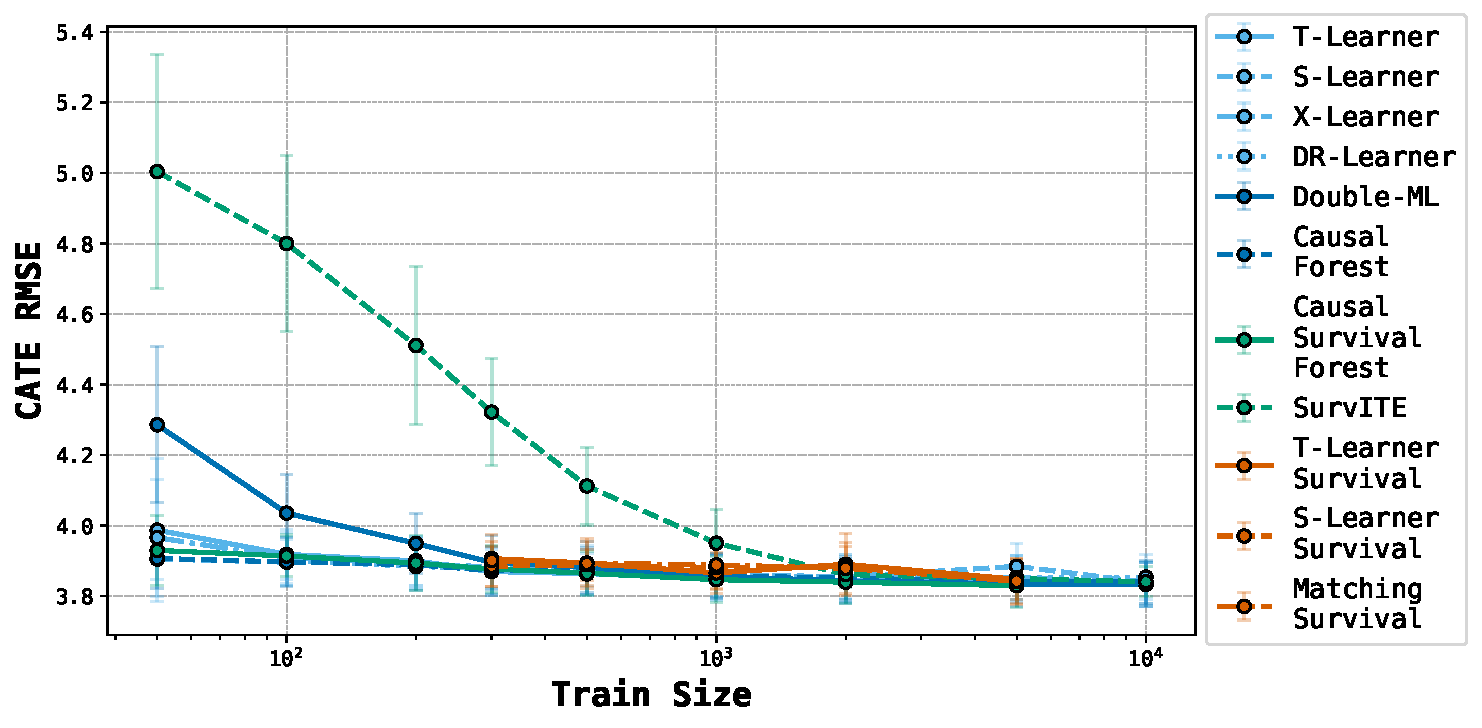
\includegraphics[width=\linewidth]{Appendices/appendix-ch04/images/figure_results_updated/convergence_results/scenario_C_RCT_0_5_convergence.pdf} 
        
    \end{minipage}}
    \hfill
    \subfloat[{RCT: \ChFourGrayCheck (5\%), Ignorability: \ChFourGrayCheck, Positivity: \ChFourGrayCheck, Ign-Censoring: \ChFourGrayCheck}]{\begin{minipage}[t]{0.49\textwidth}
        \centering
        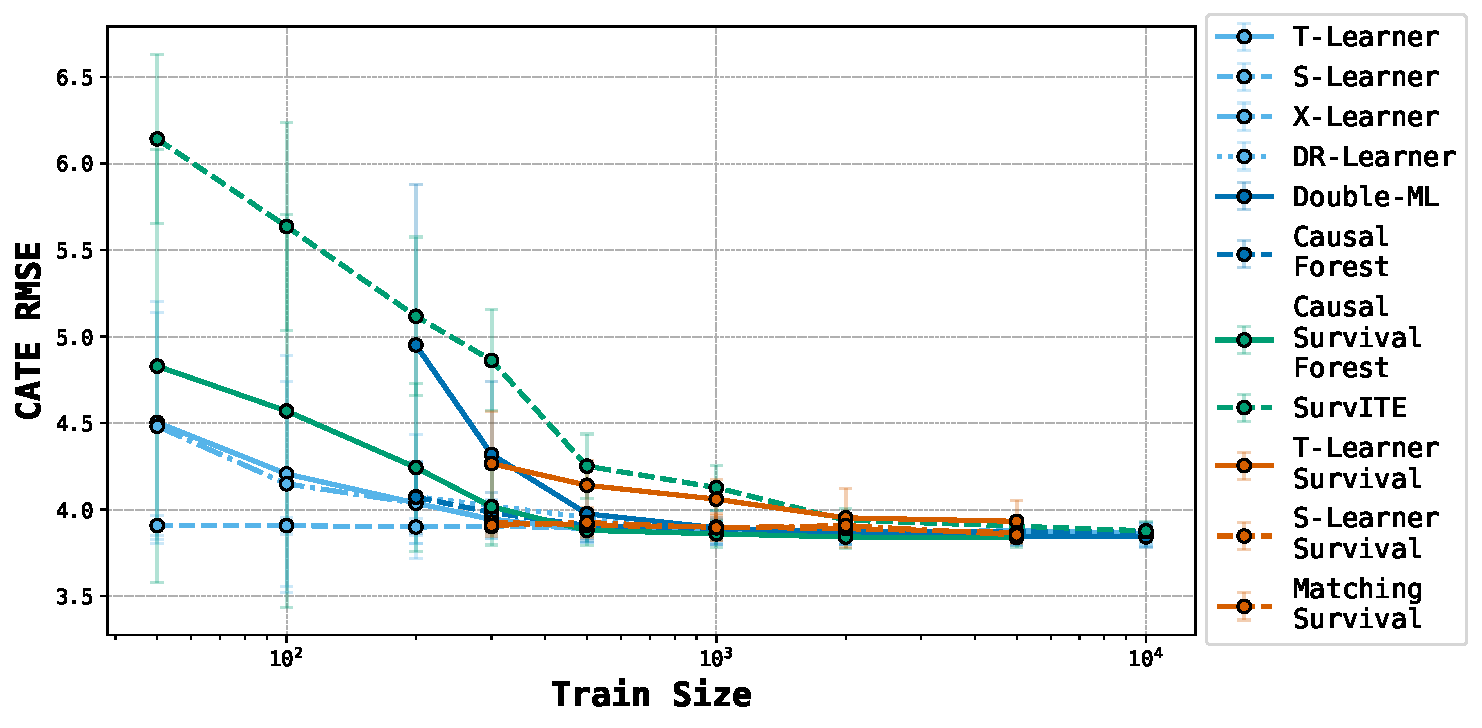
\includegraphics[width=\linewidth]{Appendices/appendix-ch04/images/figure_results_updated/convergence_results/scenario_C_RCT_0_05_convergence.pdf} 
        
    \end{minipage}}

    

    \subfloat[{RCT: \ChFourBlackCross, Ignorability: \ChFourGrayCheck, Positivity: \ChFourGrayCheck, Ignorable Censoring: \ChFourGrayCheck}]{\begin{minipage}[t]{0.49\textwidth}
        \centering
        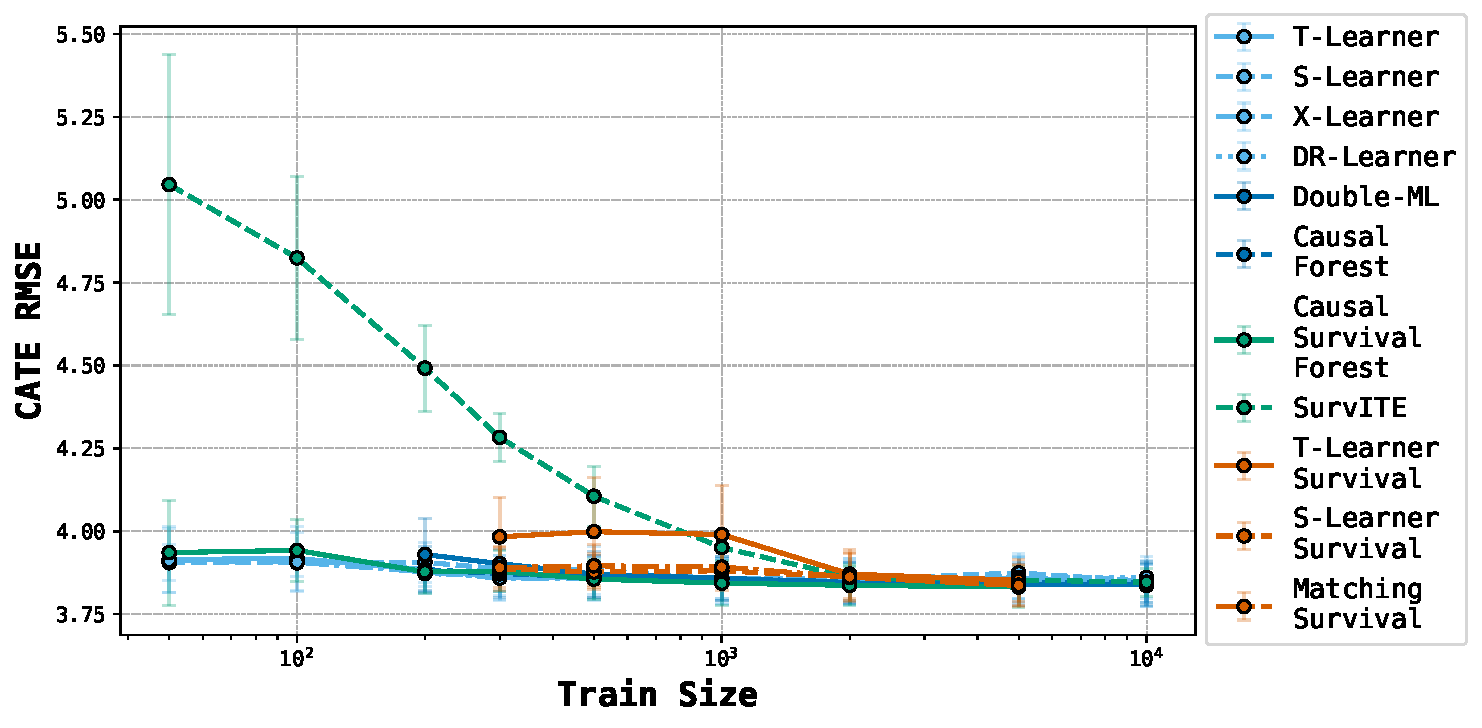
\includegraphics[width=\linewidth]{Appendices/appendix-ch04/images/figure_results_updated/convergence_results/scenario_C_e_X_convergence.pdf} 
        
    \end{minipage}}
    \hfill
    \subfloat[{RCT: \ChFourBlackCross, Ignorability: \ChFourBlackCross, Positivity: \ChFourGrayCheck, Ignorable Censoring: \ChFourGrayCheck}]{\begin{minipage}[t]{0.49\textwidth}
        \centering
        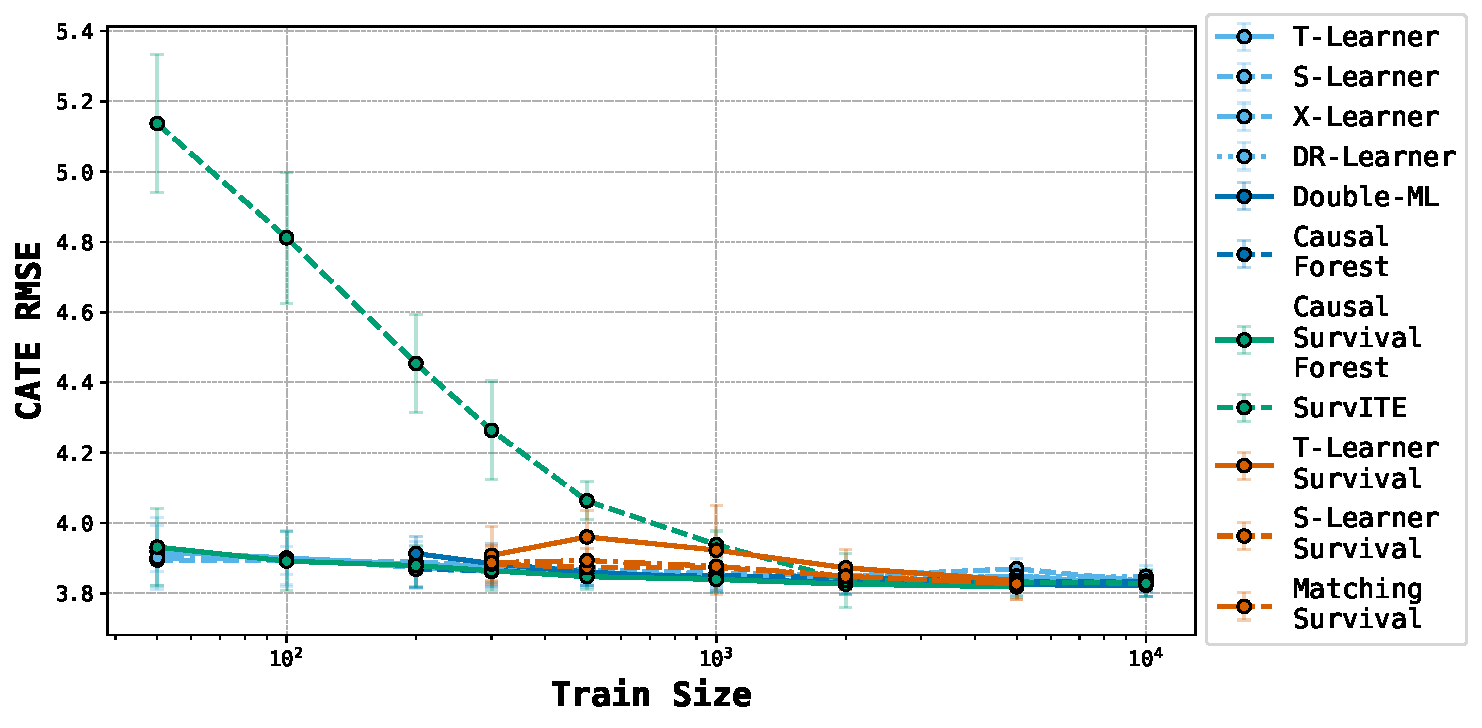
\includegraphics[width=\linewidth]{Appendices/appendix-ch04/images/figure_results_updated/convergence_results/scenario_C_e_X_U_convergence.pdf} 
        
    \end{minipage}}

    

    \subfloat[{RCT: \ChFourBlackCross, Ignorability: \ChFourGrayCheck, Positivity: \ChFourBlackCross, Ignorable Censoring: \ChFourGrayCheck}]{\begin{minipage}[t]{0.49\textwidth}
        \centering
        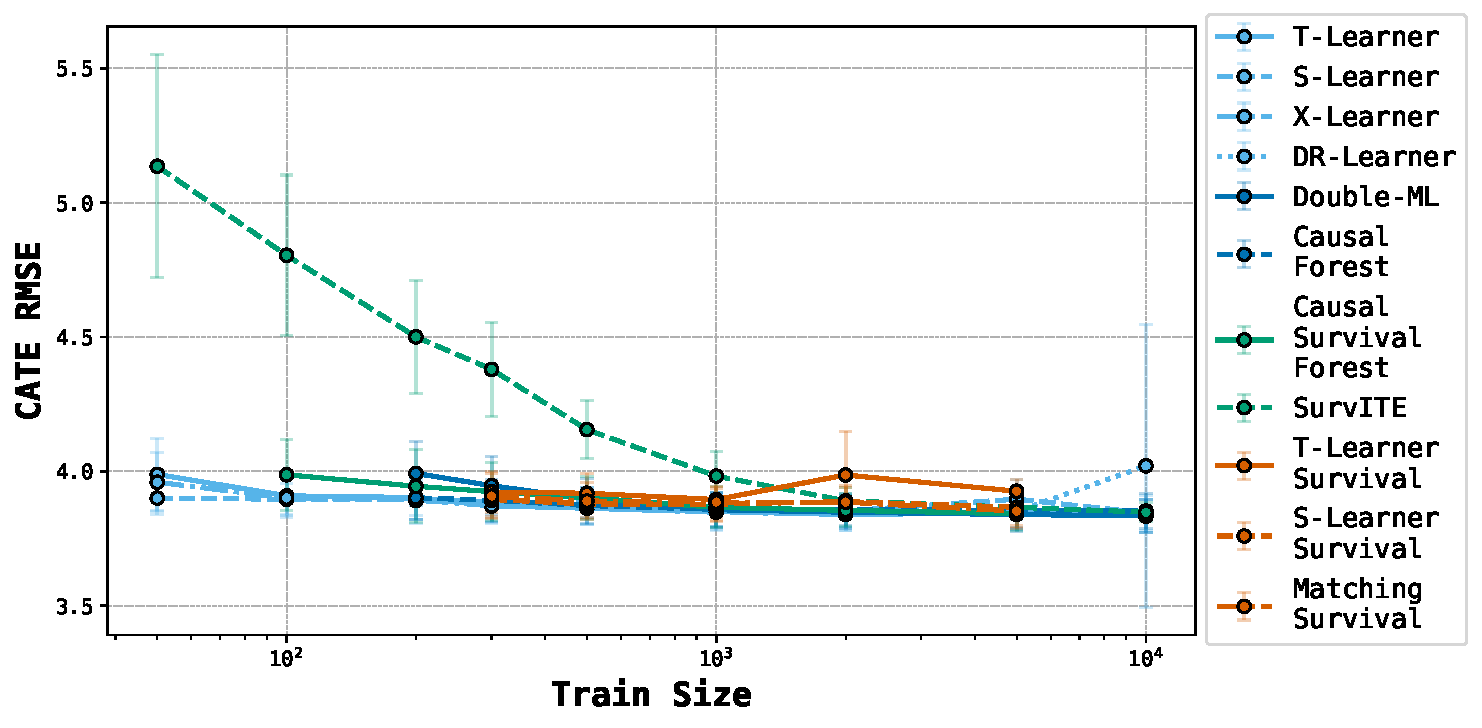
\includegraphics[width=\linewidth]{Appendices/appendix-ch04/images/figure_results_updated/convergence_results/scenario_C_e_X_no_overlap_convergence.pdf} 
        
    \end{minipage}}
    \hfill
    \subfloat[{RCT: \ChFourBlackCross, Ignorability: \ChFourGrayCheck, Positivity: \ChFourGrayCheck, Ignorable Censoring: \ChFourBlackCross}]{\begin{minipage}[t]{0.49\textwidth}
        \centering
        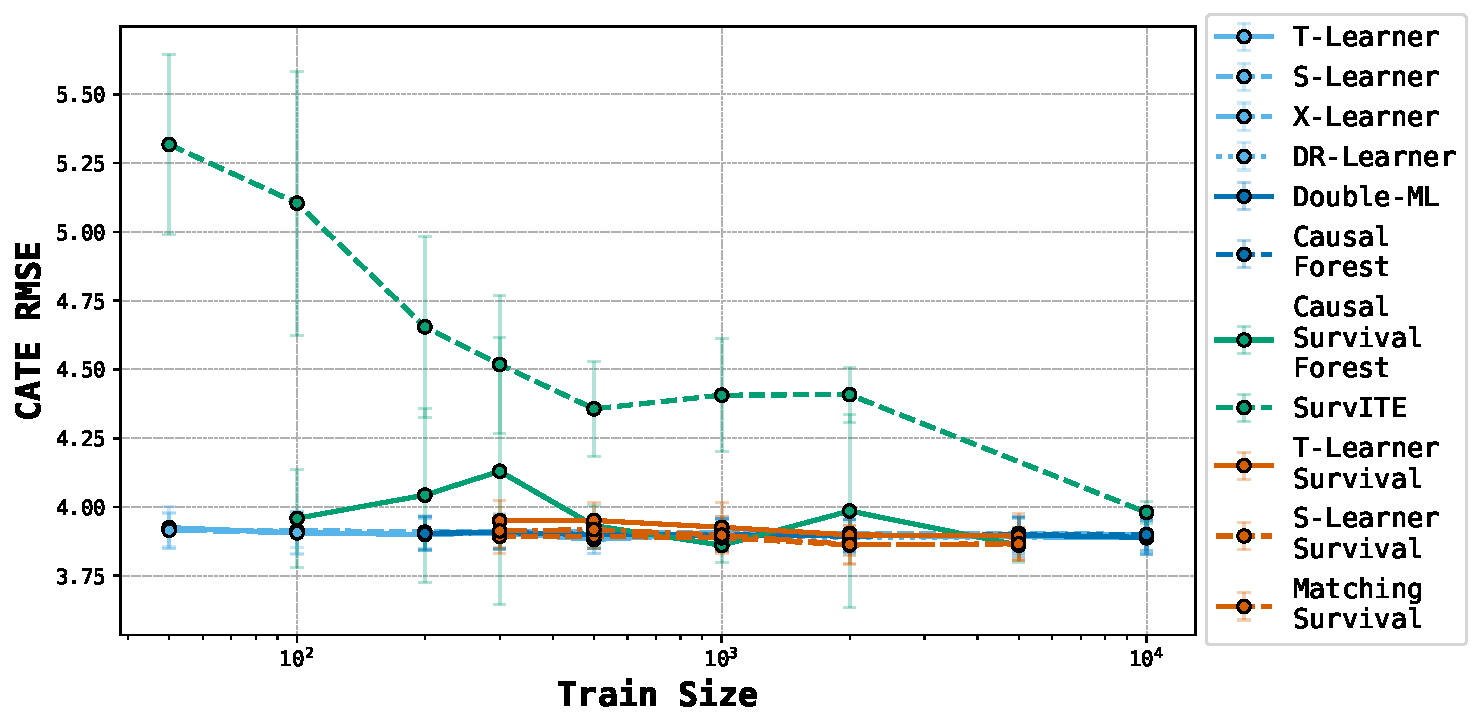
\includegraphics[width=\linewidth]{Appendices/appendix-ch04/images/figure_results_updated/convergence_results/scenario_C_e_X_info_censor_convergence.pdf} 
        
    \end{minipage}}

    

    \subfloat[{RCT: \ChFourBlackCross, Ignorability: \ChFourBlackCross, Positivity: \ChFourGrayCheck, Ignorable Censoring: \ChFourBlackCross}]{\begin{minipage}[t]{0.49\textwidth}
        \centering
        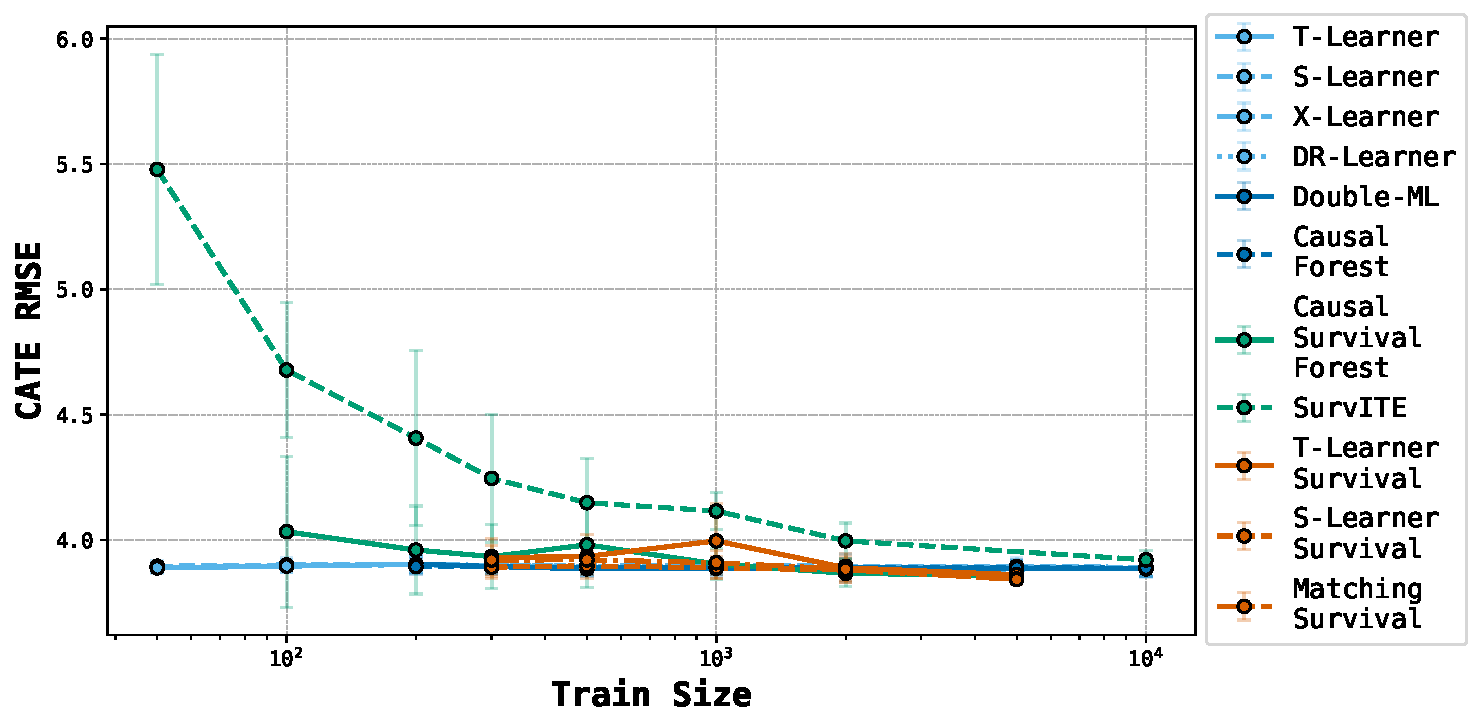
\includegraphics[width=\linewidth]{Appendices/appendix-ch04/images/figure_results_updated/convergence_results/scenario_C_e_X_U_info_censor_convergence.pdf} 
        
    \end{minipage}}
    \hfill
    \subfloat[{RCT: \ChFourBlackCross, Ignorability: \ChFourGrayCheck, Positivity: \ChFourBlackCross, Ignorable Censoring: \ChFourBlackCross}]{\begin{minipage}[t]{0.49\textwidth}
        \centering
        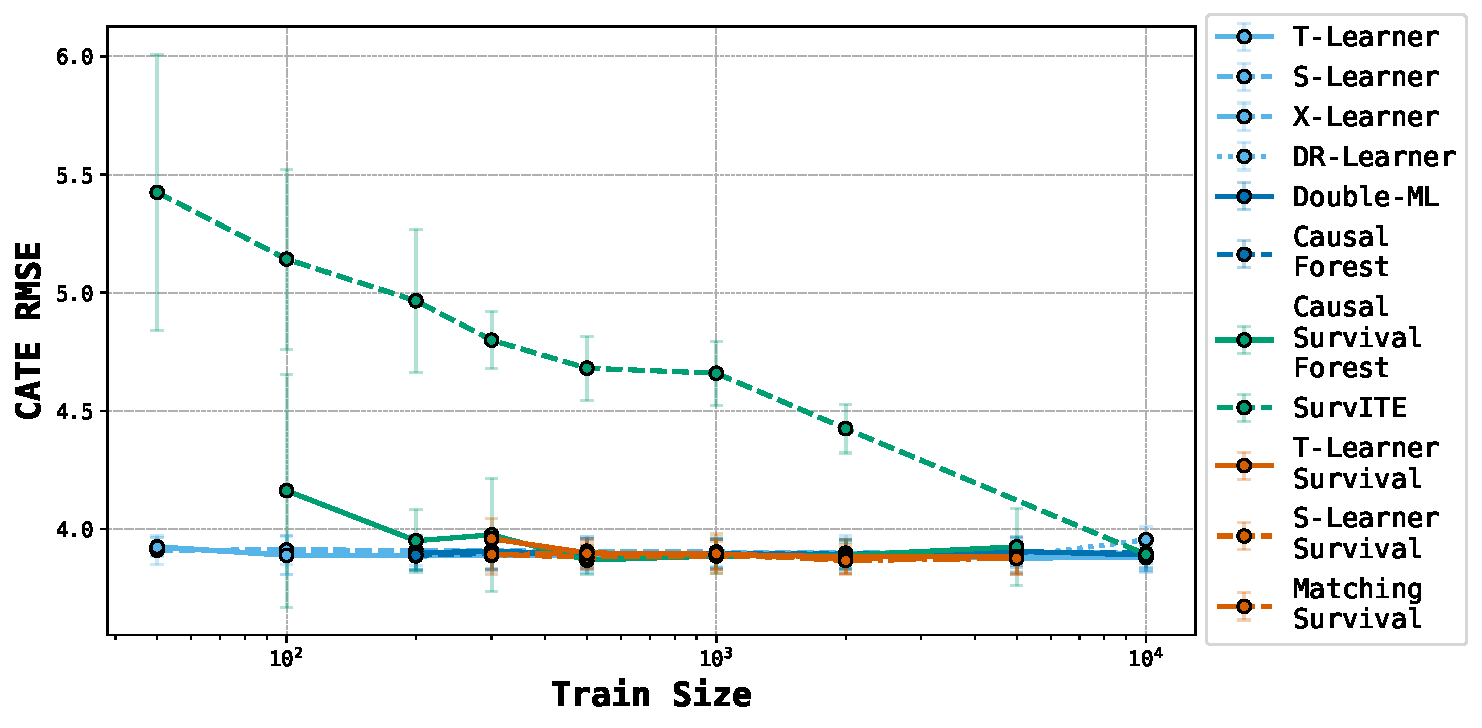
\includegraphics[width=\linewidth]{Appendices/appendix-ch04/images/figure_results_updated/convergence_results/scenario_C_e_X_no_overlap_info_censor_convergence.pdf} 
        
    \end{minipage}}

    \end{minipage}%
    }
    
    
    
}
\end{figure}




%%%%%%%%%%%%%%%%%%%%%%%%%%%%%%%%%%%%%%%%%%%%%%%%%%%%%%%%%%%%
%%%%%%%%%%%%%%%%%%%%%%%%%%%%%%%%%%%%%%%%%%%%%%%%%%%%%%%%%%%%
%%%%%%%%%%%%%%%%%%%%%%%%%%%%%%%%%%%%%%%%%%%%%%%%%%%%%%%%%%%%

